\documentclass[a4paper,10pt,titlepage]{article}

\usepackage{geometry}
\usepackage{amsmath}
\usepackage{amssymb}
\usepackage{txfonts}
\usepackage{microtype}
\usepackage{epsfig}
\usepackage{graphicx}
\usepackage{moreverb}
\usepackage{hyperref}
\usepackage{listings}
\usepackage{xcolor}
\usepackage{textcomp}
\definecolor{listinggray}{gray}{0.98}
\definecolor{lbcolor}{rgb}{0.98,0.98,0.98}
\lstset{
	backgroundcolor=\color{lbcolor},
	tabsize=4,
	rulecolor=,
	language=matlab,
    basicstyle=\scriptsize\ttfamily,
    upquote=true,
    aboveskip={1.5\baselineskip},
    columns=fixed,
    showstringspaces=false,
    extendedchars=true,
    breaklines=true,
    prebreak = \raisebox{0ex}[0ex][0ex]{\ensuremath{\hookleftarrow}},
    frame=single,
    showtabs=false,
    showspaces=false,
    showstringspaces=false,
    identifierstyle=\ttfamily,
    keywordstyle=\color[rgb]{0,0,1},
    commentstyle=\color[rgb]{0.133,0.545,0.133},
    stringstyle=\color[rgb]{0.627,0.126,0.941},
}
\usepackage{eso-pic}
\usepackage{ifthen}

\AddToShipoutPictureBG{\ifthenelse{\equal{\value{page}}{0}}{}{
\includegraphics{template_files/backgroundlines}}}


\usepackage{tikz}
\usepackage{pgfplots}
\usepackage{tikzscale}
\usepackage{graphicx}
\usepackage{float}
\usepackage{subcaption}
\usepackage{comment}
\usepackage{units}
\usetikzlibrary{external}\tikzexternalize


\title{H1a: Classical scattering by a central potential}
\author{Victor Nilsson and Simon Nilsson}
\date{\today}

\begin{document}

\newgeometry{top=2cm,bottom=2cm,left=2cm,right=2cm}

\begin{titlepage}

\setcounter{page}{0}

\begin{center}
{\huge \bf \color{red} NB: The graded, first version of the report must be
                           returned if you hand in a second time! } \\
\vspace{3cm}
\makeatletter
{ \huge \@title } \\
\vspace{1cm}
{ \Large \@author }\\
\vspace{1cm}
{ \Large \@date }\\
\makeatother
\end{center}

\vfill

\begin{flushright}
{\Large
\begin{tabular}{|c|c|c|}
\hline
Task N\textsuperscript{\underline{o}} & Points & Avail.\ points \\ \hline
\hspace{3cm} & \hspace{3cm} & \hspace{3cm} \\ \hline
~ & ~ & ~ \\ \hline
~ & ~ & ~ \\ \hline
~ & ~ & ~ \\ \hline
~ & ~ & ~ \\ \hline
~ & ~ & ~ \\ \hline
~ & ~ & ~ \\ \hline
~ & ~ & ~ \\ \hline
$\sum$ & ~ & ~ \\
\hline
\end{tabular}}
\end{flushright}

\end{titlepage}

\newgeometry{top=2cm,bottom=2cm,left=1.5cm,right=7.4cm}


\section*{Introduction}

Molecular dynamics is a simulation of the movement of atoms and molecules. What is of interest in such a simulations is e.g. the trajectories of the atoms given specific surrounding parameters such as temperature, pressure, crystal formation etc. For this homeproblem we study the dynamics of aluminium atoms in a FCC crystal lattice.

\section*{Problem 1}

\begin{figure}[H]
    \centering
    \captionsetup[subfigure]{justification=centering}
    \begin{subfigure}[b]{0.40\textwidth}
        \centering
        \resizebox{\columnwidth}{!}{% This file was created by matlab2tikz.
%
%The latest updates can be retrieved from
%  http://www.mathworks.com/matlabcentral/fileexchange/22022-matlab2tikz-matlab2tikz
%where you can also make suggestions and rate matlab2tikz.
%
\definecolor{mycolor1}{rgb}{0.00000,0.44700,0.74100}%
\definecolor{mycolor2}{rgb}{0.85000,0.32500,0.09800}%
\definecolor{mycolor3}{rgb}{0.92900,0.69400,0.12500}%
%
\begin{tikzpicture}

\begin{axis}[%
width=4.521in,
height=3.566in,
at={(0.758in,0.481in)},
scale only axis,
xmin=0,
xmax=100,
xlabel={Time / [ASU]},
ymin=-500000000,
ymax=3000000000,
ylabel={Energy / [ASU]},
axis background/.style={fill=white},
title style={font=\bfseries},
title={Awesome title},
legend style={legend cell align=left,align=left,draw=white!15!black}
]
\addplot [color=mycolor1,solid]
  table[row sep=crcr]{%
0	-857.0284\\
0.1	24095.5953\\
0.2	368482.8188\\
0.3	1345138.0751\\
0.4	2290709.7434\\
0.5	4028094.6967\\
0.6	5098138.1067\\
0.7	5828281.2084\\
0.8	6567207.687\\
0.9	7858390.8086\\
1	9842270.9262\\
1.1	12588912.0788\\
1.2	13906521.2805\\
1.3	14363649.6421\\
1.4	15127580.1113\\
1.5	16948566.4579\\
1.6	17909643.987\\
1.7	20367468.1138\\
1.8	22869417.5343\\
1.9	25193878.986\\
2	28342826.4527\\
2.1	28839450.3935\\
2.2	30331130.3247\\
2.3	32527871.7289\\
2.4	34634700.0354\\
2.5	35313003.6665\\
2.6	38613194.3993\\
2.7	48638010.5486\\
2.8	50151638.1548\\
2.9	52594947.3467\\
3	54230397.1507\\
3.1	55551364.0393\\
3.2	56353883.5097\\
3.3	56770473.197\\
3.4	57220501.7233\\
3.5	58584395.3641\\
3.6	60569094.7586\\
3.7	62692067.526\\
3.8	64324208.0889\\
3.9	65762722.5297\\
4	67438763.6942\\
4.1	69552209.7533\\
4.2	70430322.4085\\
4.3	71847176.2897\\
4.4	73325428.205\\
4.5	75173440.891\\
4.6	76403186.4331\\
4.7	78042735.9443\\
4.8	80436309.9774\\
4.9	81020332.2789\\
5	81313509.7819\\
5.1	82973294.789\\
5.2	85802275.0114\\
5.3	88124809.1011\\
5.4	89401665.4643\\
5.5	91378296.6361\\
5.6	94524164.1069\\
5.7	96460820.7844\\
5.8	99448900.6369\\
5.9	101522748.3995\\
6	102529727.8694\\
6.1	103489313.3208\\
6.2	104609660.0967\\
6.3	105365082.4452\\
6.4	105532086.5228\\
6.5	106508943.8725\\
6.6	108344488.3803\\
6.7	110121709.8413\\
6.8	111763183.3774\\
6.9	113233765.0356\\
7	116169073.1049\\
7.1	118104490.6391\\
7.2	119355631.6227\\
7.3	121436893.1461\\
7.4	125414597.4194\\
7.5	126664833.7799\\
7.6	127860903.3605\\
7.7	128494359.1918\\
7.8	131509667.0702\\
7.9	132868415.0923\\
8	135953076.5134\\
8.1	137422666.2762\\
8.2	139361879.1531\\
8.3	141303725.8262\\
8.4	142346542.104\\
8.5	142517633.7039\\
8.6	144270108.2869\\
8.7	145170602.0524\\
8.8	145451627.1261\\
8.9	147643891.664\\
9	151447749.2793\\
9.1	152875540.1467\\
9.2	153359136.4177\\
9.3	156236432.0684\\
9.4	162088141.3522\\
9.5	163921802.1429\\
9.6	165654966.0414\\
9.7	169058975.3003\\
9.8	171540103.7872\\
9.9	172046015.0507\\
10	172736806.8247\\
10.1	173685307.5643\\
10.2	175732714.4342\\
10.3	183295170.1968\\
10.4	200797840.3644\\
10.5	201756614.886\\
10.6	202525726.5692\\
10.7	203422576.5659\\
10.8	203624812.4169\\
10.9	205182760.1219\\
11	207087252.9362\\
11.1	208871185.2308\\
11.2	210006366.1458\\
11.3	210255337.3167\\
11.4	210892225.7987\\
11.5	211806782.2698\\
11.6	212371310.8326\\
11.7	211843505.3813\\
11.8	211416643.4093\\
11.9	212026648.1661\\
12	214093501.2604\\
12.1	216844292.7644\\
12.2	217815810.938\\
12.3	221439033.8285\\
12.4	225262649.954\\
12.5	225909529.3479\\
12.6	236861155.3667\\
12.7	275089737.4125\\
12.8	275934219.2462\\
12.9	277004785.0409\\
13	279092318.4577\\
13.1	280791193.7368\\
13.2	282402272.2673\\
13.3	283471815.5033\\
13.4	283847235.4979\\
13.5	284676749.7207\\
13.6	286699415.3881\\
13.7	289321199.1244\\
13.8	289394353.1631\\
13.9	288548264.4833\\
14	288333036.0154\\
14.1	290495916.6402\\
14.2	293607656.5212\\
14.3	293674332.2067\\
14.4	293411859.06\\
14.5	294030063.2744\\
14.6	295972105.0342\\
14.7	298374422.487\\
14.8	298514850.4058\\
14.9	299809775.5186\\
15	301295545.5831\\
15.1	301679837.5417\\
15.2	301860737.5009\\
15.3	303144766.5294\\
15.4	302825554.9364\\
15.5	304036624.4536\\
15.6	306718791.1735\\
15.7	308355795.3564\\
15.8	309576938.3408\\
15.9	310345230.2321\\
16	311016053.1378\\
16.1	312132047.8506\\
16.2	312627741.0367\\
16.3	311755558.0128\\
16.4	320523105.8083\\
16.5	320510118.3786\\
16.6	323311961.732\\
16.7	330599491.7075\\
16.8	332636466.8764\\
16.9	339348531.9854\\
17	341513488.8474\\
17.1	348059683.4214\\
17.2	358403752.4416\\
17.3	359870723.2124\\
17.4	360714889.1072\\
17.5	361480827.9965\\
17.6	363364939.7069\\
17.7	363760352.8321\\
17.8	364060902.6576\\
17.9	369031431.9849\\
18	381228445.3508\\
18.1	383351806.6154\\
18.2	388212224.3701\\
18.3	388988339.4032\\
18.4	391771464.5376\\
18.5	394362065.1893\\
18.6	395646513.8304\\
18.7	397945075.0721\\
18.8	398553259.5309\\
18.9	398321093.9276\\
19	400935192.1199\\
19.1	402946871.2045\\
19.2	403766205.1315\\
19.3	405453707.4409\\
19.4	407301724.8853\\
19.5	409720817.2219\\
19.6	416568717.5284\\
19.7	424105779.7432\\
19.8	425676240.9535\\
19.9	427654736.783\\
20	429356679.8849\\
20.1	431715546.8356\\
20.2	434805900.0159\\
20.3	437406645.8773\\
20.4	437919276.065\\
20.5	438375024.8556\\
20.6	438841242.6693\\
20.7	442556269.4132\\
20.8	443977557.2853\\
20.9	446017862.1335\\
21	451845473.2756\\
21.1	456739353.0559\\
21.2	456658388.8079\\
21.3	457840365.3658\\
21.4	459058450.6133\\
21.5	458423564.0334\\
21.6	457393070.5846\\
21.7	456942850.7216\\
21.8	461463687.0176\\
21.9	471061340.7374\\
22	477202160.4461\\
22.1	478705123.4672\\
22.2	488435615.8222\\
22.3	521134981.0696\\
22.4	525049019.8306\\
22.5	525474981.6925\\
22.6	525181723.6958\\
22.7	526417843.8027\\
22.8	527317635.2691\\
22.9	525803314.7795\\
23	525764500.8714\\
23.1	527336477.7655\\
23.2	529916180.0102\\
23.3	534508518.1266\\
23.4	537383594.8652\\
23.5	537774918.8335\\
23.6	539073024.5557\\
23.7	542718243.4654\\
23.8	544188970.7669\\
23.9	545942054.7526\\
24	548359291.4185\\
24.1	554984302.5747\\
24.2	570380538.2067\\
24.3	574466807.6143\\
24.4	577988845.9245\\
24.5	578011702.5423\\
24.6	578411579.2878\\
24.7	584428220.5503\\
24.8	590404924.9629\\
24.9	592073848.1824\\
25	596574298.5346\\
25.1	598317854.493\\
25.2	599923718.9772\\
25.3	602991148.2013\\
25.4	609029281.9493\\
25.5	610031740.62\\
25.6	611783496.9415\\
25.7	614356030.7938\\
25.8	619762472.5001\\
25.9	621313001.1378\\
26	626824961.0616\\
26.1	631028428.1747\\
26.2	632975536.4658\\
26.3	637317503.4272\\
26.4	636857881.1961\\
26.5	640885312.7721\\
26.6	655547155.7677\\
26.7	656108625.5827\\
26.8	660550256.6189\\
26.9	670945302.9953\\
27	672082068.7472\\
27.1	672337396.2293\\
27.2	671588972.3386\\
27.3	674636400.8144\\
27.4	689615127.006\\
27.5	690628514.6705\\
27.6	691288078.0049\\
27.7	694490135.2191\\
27.8	696457350.5842\\
27.9	698949610.3248\\
28	701081983.0886\\
28.1	701110476.7211\\
28.2	701327930.5326\\
28.3	706913668.0548\\
28.4	712393100.5709\\
28.5	713844809.6817\\
28.6	716711771.8375\\
28.7	733503045.282\\
28.8	772833419.3031\\
28.9	771801807.2403\\
29	773249530.5513\\
29.1	775772936.9942\\
29.2	775875972.0667\\
29.3	776131906.6816\\
29.4	776892489.8246\\
29.5	778718693.8248\\
29.6	782384381.4187\\
29.7	783736132.0822\\
29.8	784526552.9683\\
29.9	797055720.9875\\
30	828863502.7653\\
30.1	832206763.1577\\
30.2	836010140.576\\
30.3	839251587.7727\\
30.4	840305339.1744\\
30.5	840682339.2226\\
30.6	843107040.3349\\
30.7	843385574.657\\
30.8	850170535.9814\\
30.9	860510453.4279\\
31	864409603.9424\\
31.1	865876117.8453\\
31.2	867386709.6148\\
31.3	869203327.748\\
31.4	871660151.9729\\
31.5	872530483.7138\\
31.6	871793126.0492\\
31.7	872529825.1074\\
31.8	877423351.038\\
31.9	879501291.4968\\
32	884453700.0664\\
32.1	890333747.4335\\
32.2	892744598.2947\\
32.3	892568006.1555\\
32.4	892965184.5267\\
32.5	895343971.8646\\
32.6	897992503.3279\\
32.7	908114588.1794\\
32.8	925772853.2226\\
32.9	933854707.6963\\
33	949296104.0365\\
33.1	955990115.2917\\
33.2	980614635.9956\\
33.3	982956699.6002\\
33.4	983319565.2633\\
33.5	986299351.8147\\
33.6	992092337.6188\\
33.7	991302294.2488\\
33.8	991762740.7527\\
33.9	993054676.6995\\
34	993696786.4112\\
34.1	1001540458.5562\\
34.2	1015023931.4902\\
34.3	1015780728.1515\\
34.4	1016751732.9899\\
34.5	1019171647.4592\\
34.6	1022140667.5181\\
34.7	1022564790.1363\\
34.8	1023121233.6162\\
34.9	1024806163.2327\\
35	1028785406.0861\\
35.1	1032874669.3947\\
35.2	1037902989.3754\\
35.3	1046999064.6373\\
35.4	1064123329.8069\\
35.5	1071087316.5087\\
35.6	1075257695.2999\\
35.7	1081634225.8557\\
35.8	1081537325.4367\\
35.9	1081490625.2059\\
36	1082733629.2658\\
36.1	1085170346.9647\\
36.2	1085906372.6815\\
36.3	1086549615.8606\\
36.4	1088138541.4471\\
36.5	1088233421.2993\\
36.6	1088943423.4032\\
36.7	1089245190.3235\\
36.8	1089039622.9145\\
36.9	1091880696.7371\\
37	1095410000.5298\\
37.1	1098402579.7476\\
37.2	1104354511.817\\
37.3	1117948195.279\\
37.4	1116979530.3162\\
37.5	1123491614.956\\
37.6	1129826667.4575\\
37.7	1127242691.2529\\
37.8	1126277576.0817\\
37.9	1127917017.3167\\
38	1129778620.1831\\
38.1	1132234809.5226\\
38.2	1130428043.9069\\
38.3	1130496227.3817\\
38.4	1131174434.0119\\
38.5	1131264677.5964\\
38.6	1130486941.4946\\
38.7	1127698748.6321\\
38.8	1128346731.9458\\
38.9	1131207661.5838\\
39	1141213078.9854\\
39.1	1144948798.7074\\
39.2	1148742653.1097\\
39.3	1156374927.7691\\
39.4	1167012101.9759\\
39.5	1169185376.6521\\
39.6	1168393917.0665\\
39.7	1171038776.8607\\
39.8	1181978944.4663\\
39.9	1186827991.0393\\
40	1185727429.7074\\
40.1	1189182735.0074\\
40.2	1195278690.2982\\
40.3	1196886524.4249\\
40.4	1198648024.67\\
40.5	1192796864.775\\
40.6	1194533946.9225\\
40.7	1197305763.4108\\
40.8	1199186418.4767\\
40.9	1198366068.7345\\
41	1197631024.4088\\
41.1	1198619882.67\\
41.2	1200638965.4908\\
41.3	1200729070.0593\\
41.4	1201487189.6697\\
41.5	1203977473.9469\\
41.6	1206406568.1025\\
41.7	1210202362.2478\\
41.8	1213299184.6702\\
41.9	1212344590.2116\\
42	1215113236.2315\\
42.1	1215191825.4085\\
42.2	1216120725.3947\\
42.3	1218305612.3715\\
42.4	1219545917.3518\\
42.5	1219974041.1196\\
42.6	1225819202.712\\
42.7	1238988956.5514\\
42.8	1241912797.8186\\
42.9	1244002905.1901\\
43	1243897355.8998\\
43.1	1243362306.2283\\
43.2	1242351055.3611\\
43.3	1244611985.3436\\
43.4	1248910405.6713\\
43.5	1251826949.749\\
43.6	1256472603.5017\\
43.7	1262531021.5702\\
43.8	1266729073.6775\\
43.9	1269107209.485\\
44	1271268898.1432\\
44.1	1274033405.3749\\
44.2	1275725984.3999\\
44.3	1274935965.3726\\
44.4	1277750788.7505\\
44.5	1279049902.8241\\
44.6	1279731645.9033\\
44.7	1282409681.6605\\
44.8	1288971626.2074\\
44.9	1296112957.6328\\
45	1306311802.2639\\
45.1	1306897043.9519\\
45.2	1308305152.5801\\
45.3	1308825768.5881\\
45.4	1309664897.3785\\
45.5	1310650990.2206\\
45.6	1312144672.6092\\
45.7	1311907227.3521\\
45.8	1311878248.857\\
45.9	1312294749.7377\\
46	1314506323.6148\\
46.1	1319556658.1277\\
46.2	1316967424.7274\\
46.3	1316987108.8967\\
46.4	1315940881.7247\\
46.5	1314444362.637\\
46.6	1315499997.7259\\
46.7	1315409004.103\\
46.8	1314508259.6215\\
46.9	1312090102.5915\\
47	1311962730.6328\\
47.1	1313805624.704\\
47.2	1316683052.7597\\
47.3	1312551715.4708\\
47.4	1313508016.3639\\
47.5	1311186891.996\\
47.6	1311092266.0061\\
47.7	1311549870.5431\\
47.8	1310248024.0236\\
47.9	1312142260.9733\\
48	1314713527.7055\\
48.1	1313999488.5716\\
48.2	1314652622.6918\\
48.3	1319787940.6103\\
48.4	1321506241.1643\\
48.5	1322547862.3009\\
48.6	1325398673.2799\\
48.7	1325871192.1294\\
48.8	1326012716.1465\\
48.9	1327923115.2179\\
49	1328454457.0001\\
49.1	1331951614.497\\
49.2	1337515103.1719\\
49.3	1337928896.5122\\
49.4	1340476160.5973\\
49.5	1344285019.8106\\
49.6	1346677004.0363\\
49.7	1350677681.9634\\
49.8	1352534760.33\\
49.9	1355737396.0907\\
50	1358506912.3453\\
50.1	1361089515.5233\\
50.2	1367286016.499\\
50.3	1370310724.5288\\
50.4	1370444119.9211\\
50.5	1372131811.6979\\
50.6	1374299860.6575\\
50.7	1376566877.0535\\
50.8	1376057202.834\\
50.9	1374983351.6992\\
51	1372916186.0439\\
51.1	1372282905.2523\\
51.2	1373979585.2589\\
51.3	1376785609.1131\\
51.4	1380074831.4843\\
51.5	1381372875.1168\\
51.6	1379776062.2553\\
51.7	1380415047.6136\\
51.8	1388955414.5982\\
51.9	1393510674.645\\
52	1397852387.5043\\
52.1	1396184032.1842\\
52.2	1396140507.7996\\
52.3	1400861719.1963\\
52.4	1402922048.3966\\
52.5	1405428127.3913\\
52.6	1408371775.7299\\
52.7	1411840610.0701\\
52.8	1413871343.9289\\
52.9	1414359854.588\\
53	1414450117.1929\\
53.1	1417937604.4933\\
53.2	1420662194.9537\\
53.3	1421263226.0935\\
53.4	1423513029.7296\\
53.5	1428353715.775\\
53.6	1434627586.5977\\
53.7	1437403939.1629\\
53.8	1439344967.0444\\
53.9	1438601600.2968\\
54	1437946555.9644\\
54.1	1438516371.9432\\
54.2	1444208033.5085\\
54.3	1450451803.7732\\
54.4	1450900280.3903\\
54.5	1456747364.0809\\
54.6	1469253633.6896\\
54.7	1475079729.293\\
54.8	1476689827.7538\\
54.9	1479544382.5388\\
55	1477743310.4021\\
55.1	1476858897.7627\\
55.2	1478991578.2506\\
55.3	1480889509.7309\\
55.4	1483293000.1857\\
55.5	1486630151.5665\\
55.6	1487906523.5372\\
55.7	1490092851.8804\\
55.8	1492800231.5284\\
55.9	1496897967.4567\\
56	1503447022.234\\
56.1	1510886324.5957\\
56.2	1515183534.6352\\
56.3	1515684323.2082\\
56.4	1530421868.5792\\
56.5	1526182007.037\\
56.6	1534658709.8211\\
56.7	1535475889.8426\\
56.8	1541542492.7064\\
56.9	1547079000.1211\\
57	1548295552.814\\
57.1	1548977612.2583\\
57.2	1550517853.3667\\
57.3	1551567178.0123\\
57.4	1544415794.2953\\
57.5	1537995008.0477\\
57.6	1536248653.3148\\
57.7	1537554615.6633\\
57.8	1541162988.5994\\
57.9	1541257172.7403\\
58	1539860591.511\\
58.1	1541696881.3501\\
58.2	1540714835.7386\\
58.3	1543763790.9764\\
58.4	1546414356.4385\\
58.5	1548996991.9442\\
58.6	1548506763.7937\\
58.7	1548671008.6344\\
58.8	1551001122.2898\\
58.9	1554247429.9202\\
59	1556755475.2099\\
59.1	1558813759.8915\\
59.2	1558719716.0389\\
59.3	1557569666.0419\\
59.4	1560291380.2985\\
59.5	1563815177.649\\
59.6	1561257314.3897\\
59.7	1561727147.6682\\
59.8	1564100843.9501\\
59.9	1564587019.8964\\
60	1567084133.0583\\
60.1	1570006783.2394\\
60.2	1571853985.0856\\
60.3	1574024327.6358\\
60.4	1579612594.9361\\
60.5	1584022132.4276\\
60.6	1583149544.9859\\
60.7	1591504915.7737\\
60.8	1603202057.7673\\
60.9	1602037555.3889\\
61	1604509829.757\\
61.1	1605798508.587\\
61.2	1604865004.826\\
61.3	1604001667.8196\\
61.4	1604406063.5145\\
61.5	1606526755.6253\\
61.6	1599173580.0047\\
61.7	1608972379.3194\\
61.8	1607949752.9882\\
61.9	1609001590.2422\\
62	1611049024.0355\\
62.1	1610769991.5533\\
62.2	1618388204.7204\\
62.3	1630058140.5457\\
62.4	1634027790.8576\\
62.5	1637746198.1754\\
62.6	1640729532.5749\\
62.7	1643588402.1267\\
62.8	1648205186.1575\\
62.9	1650716427.2161\\
63	1649484764.3946\\
63.1	1647460595.6766\\
63.2	1649475669.4122\\
63.3	1650836844.2628\\
63.4	1656676435.5714\\
63.5	1652085303.9649\\
63.6	1645068372.3408\\
63.7	1641750946.1122\\
63.8	1642898536.6467\\
63.9	1644777481.4389\\
64	1643831061.1389\\
64.1	1637509100.3363\\
64.2	1639954745.7417\\
64.3	1642545817.3164\\
64.4	1643777305.6185\\
64.5	1649052047.8071\\
64.6	1648758501.8872\\
64.7	1647202533.0142\\
64.8	1646086494.2279\\
64.9	1645301065.1324\\
65	1643518394.7243\\
65.1	1646983044.4075\\
65.2	1644522953.7125\\
65.3	1640736757.7926\\
65.4	1640789416.2161\\
65.5	1651678603.7729\\
65.6	1665133849.2297\\
65.7	1665875072.9505\\
65.8	1664834175.6125\\
65.9	1666196728.8044\\
66	1673395631.6711\\
66.1	1682481219.9649\\
66.2	1685683257.3731\\
66.3	1687475995.58\\
66.4	1689294625.5502\\
66.5	1690480936.1731\\
66.6	1689785241.8723\\
66.7	1692005246.3614\\
66.8	1697801921.4298\\
66.9	1700409752.3069\\
67	1707822413.3719\\
67.1	1720961738.8101\\
67.2	1725543641.7828\\
67.3	1728367246.4533\\
67.4	1729825154.5918\\
67.5	1731921791.8515\\
67.6	1739397315.4896\\
67.7	1746004680.2339\\
67.8	1753909409.6571\\
67.9	1767317968.1157\\
68	1774404754.5251\\
68.1	1773425377.3414\\
68.2	1774115264.6113\\
68.3	1777219017.164\\
68.4	1784591530.6052\\
68.5	1792052895.1885\\
68.6	1793513549.8149\\
68.7	1795373826.1081\\
68.8	1798869428.2401\\
68.9	1804217881.6912\\
69	1805114086.6037\\
69.1	1808517665.3892\\
69.2	1810823114.0657\\
69.3	1810891588.445\\
69.4	1809285962.3625\\
69.5	1810562232.5757\\
69.6	1814092611.5244\\
69.7	1814147450.4025\\
69.8	1818905920.875\\
69.9	1823922463.6926\\
70	1830286157.5843\\
70.1	1834876575.1751\\
70.2	1833906903.7975\\
70.3	1836045605.9891\\
70.4	1840951420.4946\\
70.5	1843905307.5169\\
70.6	1841454580.6111\\
70.7	1840562427.6949\\
70.8	1841658293.4687\\
70.9	1846466521.8144\\
71	1845780592.5896\\
71.1	1844106467.8787\\
71.2	1844117895.7581\\
71.3	1846042458.6235\\
71.4	1846226978.1287\\
71.5	1845858767.6191\\
71.6	1848015224.1116\\
71.7	1848937448.1653\\
71.8	1850183424.5598\\
71.9	1850945907.3649\\
72	1852761174.5429\\
72.1	1856033024.1775\\
72.2	1854944088.7283\\
72.3	1855192689.4453\\
72.4	1855415407.363\\
72.5	1855520608.5626\\
72.6	1855334487.5862\\
72.7	1857856031.4503\\
72.8	1861959653.0525\\
72.9	1865181942.2578\\
73	1863292849.768\\
73.1	1870472196.9098\\
73.2	1885442582.0068\\
73.3	1886427694.4611\\
73.4	1889659075.0368\\
73.5	1892850018.1758\\
73.6	1888945659.4234\\
73.7	1888740997.5047\\
73.8	1891715634.3958\\
73.9	1893194068.7043\\
74	1893856538.8091\\
74.1	1892293977.8561\\
74.2	1889609832.9644\\
74.3	1890922919.3732\\
74.4	1892544500.9575\\
74.5	1897331996.7435\\
74.6	1906119244.2767\\
74.7	1908247083.6038\\
74.8	1908458736.6136\\
74.9	1910545419.3166\\
75	1917496251.0133\\
75.1	1926696380.9182\\
75.2	1930920933.6591\\
75.3	1936547014.0836\\
75.4	1940007644.0649\\
75.5	1944059548.8681\\
75.6	1943986203.3649\\
75.7	1944134788.2432\\
75.8	1946803298.5569\\
75.9	1945479553.0443\\
76	1942811686.9705\\
76.1	1943213454.2021\\
76.2	1942576773.5806\\
76.3	1942816517.6378\\
76.4	1945954979.8581\\
76.5	1950048285.5243\\
76.6	1958580937.2508\\
76.7	1966087290.7549\\
76.8	1969489753.8198\\
76.9	1969848494.7049\\
77	1966988521.8671\\
77.1	1965679292.747\\
77.2	1968865294.9065\\
77.3	1970871744.9747\\
77.4	1977831886.0646\\
77.5	1982025659.3659\\
77.6	1981616171.3528\\
77.7	1979169189.5795\\
77.8	1980806881.2203\\
77.9	1981896094.4707\\
78	1981150322.4186\\
78.1	1981800765.7552\\
78.2	1982735524.4444\\
78.3	1982754407.2451\\
78.4	1982470816.9742\\
78.5	1985451673.7237\\
78.6	1988495947.7035\\
78.7	1989918424.7671\\
78.8	1989188477.7972\\
78.9	1987948173.6701\\
79	1992454027.4466\\
79.1	1999294664.9269\\
79.2	2006035052.8997\\
79.3	2020081690.9604\\
79.4	2021551875.7604\\
79.5	2022935809.5872\\
79.6	2024699096.5097\\
79.7	2025001472.889\\
79.8	2023076182.1583\\
79.9	2030568785.8913\\
80	2041752520.8657\\
80.1	2040351509.5251\\
80.2	2042983086.797\\
80.3	2046898440.9229\\
80.4	2044500054.9103\\
80.5	2041141109.99\\
80.6	2041698806.0314\\
80.7	2044850644.2062\\
80.8	2042698908.355\\
80.9	2039896243.5281\\
81	2037658153.6513\\
81.1	2036465289.0906\\
81.2	2039541252.3019\\
81.3	2043696710.0186\\
81.4	2043276699.1607\\
81.5	2044725575.592\\
81.6	2048606675.2547\\
81.7	2049071006.3786\\
81.8	2048137872.9761\\
81.9	2043923412.1441\\
82	2042831194.9546\\
82.1	2041065895.3898\\
82.2	2040774504.834\\
82.3	2043756921.8946\\
82.4	2042570979.5684\\
82.5	2043948713.9059\\
82.6	2045755375.8652\\
82.7	2045923198.0926\\
82.8	2047161665.9772\\
82.9	2045211874.0124\\
83	2040081213.5504\\
83.1	2040636768.0139\\
83.2	2043099401.639\\
83.3	2045478915.5034\\
83.4	2048461416.1856\\
83.5	2050879071.4479\\
83.6	2052658484.967\\
83.7	2054476910.3055\\
83.8	2056008560.416\\
83.9	2058044639.0081\\
84	2057283279.7193\\
84.1	2055288367.9109\\
84.2	2055251597.2935\\
84.3	2056893600.1729\\
84.4	2058031736.4433\\
84.5	2060305776.9766\\
84.6	2060992945.7848\\
84.7	2059191712.7549\\
84.8	2060091308.7848\\
84.9	2064847179.9934\\
85	2065164733.1657\\
85.1	2066931059.1557\\
85.2	2073450170.0216\\
85.3	2075757910.9707\\
85.4	2078991518.614\\
85.5	2086538643.3015\\
85.6	2088810276.1318\\
85.7	2090695152.2586\\
85.8	2088377410.6648\\
85.9	2090870684.1265\\
86	2096158853.9069\\
86.1	2102326796.9347\\
86.2	2104127203.6353\\
86.3	2099208391.0837\\
86.4	2103703327.422\\
86.5	2105398137.6703\\
86.6	2107216620.3532\\
86.7	2108018305.8731\\
86.8	2104903671.5649\\
86.9	2103605989.7349\\
87	2108213898.1034\\
87.1	2113475070.1552\\
87.2	2114108843.513\\
87.3	2120425823.7671\\
87.4	2126059141.5792\\
87.5	2122526207.9867\\
87.6	2121213543.0533\\
87.7	2122162819.5219\\
87.8	2124868208.0462\\
87.9	2135504152.2251\\
88	2140714743.45\\
88.1	2138161348.9777\\
88.2	2138860851.7837\\
88.3	2142290040.7915\\
88.4	2138548140.5887\\
88.5	2137930170.4841\\
88.6	2142263610.7945\\
88.7	2148706922.2026\\
88.8	2153717290.4605\\
88.9	2155688957.3963\\
89	2186426103.3062\\
89.1	2255848590.8376\\
89.2	2256569837.8611\\
89.3	2248656774.0002\\
89.4	2242207301.4437\\
89.5	2244830384.9439\\
89.6	2243653057.9268\\
89.7	2239417211.3556\\
89.8	2237876498.0279\\
89.9	2237668600.4328\\
90	2238172071.8273\\
90.1	2239568659.5222\\
90.2	2241671616.4708\\
90.3	2239866302.7541\\
90.4	2239084892.589\\
90.5	2238944186.2675\\
90.6	2237865891.6053\\
90.7	2240624645.0122\\
90.8	2245822016.0347\\
90.9	2247445402.8937\\
91	2247046090.1738\\
91.1	2251381843.5307\\
91.2	2264213109.6546\\
91.3	2268958912.215\\
91.4	2274240909.022\\
91.5	2277585308.4409\\
91.6	2281812282.3187\\
91.7	2286357363.4844\\
91.8	2288588337.7288\\
91.9	2290228116.8962\\
92	2301631154.6009\\
92.1	2337272629.9255\\
92.2	2332599650.7904\\
92.3	2330639672.5383\\
92.4	2330546795.6919\\
92.5	2330820718.5566\\
92.6	2327525609.9252\\
92.7	2326339155.2578\\
92.8	2334933482.7147\\
92.9	2355444458.8729\\
93	2359491849.2238\\
93.1	2359366681.9672\\
93.2	2362181059.0864\\
93.3	2365303004.539\\
93.4	2372819520.6125\\
93.5	2379927810.3876\\
93.6	2381780271.9991\\
93.7	2385715110.9694\\
93.8	2390900603.8042\\
93.9	2392892988.2466\\
94	2389090656.8036\\
94.1	2387275756.6748\\
94.2	2385726900.281\\
94.3	2382616713.4412\\
94.4	2379724076.2682\\
94.5	2380589573.0291\\
94.6	2384809351.4148\\
94.7	2386513804.8236\\
94.8	2387316574.8983\\
94.9	2392097186.4756\\
95	2394342158.0036\\
95.1	2395661921.6573\\
95.2	2396195773.3245\\
95.3	2396488469.5997\\
95.4	2396079182.0188\\
95.5	2398295100.6444\\
95.6	2403261442.12\\
95.7	2406278970.0452\\
95.8	2410223745.2658\\
95.9	2413997949.8463\\
96	2417192988.0392\\
96.1	2420331432.9727\\
96.2	2429484546.4172\\
96.3	2438413698.6497\\
96.4	2439547707.6858\\
96.5	2438692207.4484\\
96.6	2439318171.1559\\
96.7	2442481475.1183\\
96.8	2443917127.7291\\
96.9	2447237096.3054\\
97	2450379055.586\\
97.1	2455752880.7046\\
97.2	2463421725.768\\
97.3	2468716584.0427\\
97.4	2473394218.3513\\
97.5	2475644416.1858\\
97.6	2475421301.0923\\
97.7	2479615930.9289\\
97.8	2480707742.5339\\
97.9	2479824636.866\\
98	2479124407.4117\\
98.1	2476014830.6727\\
98.2	2474358998.3288\\
98.3	2476628489.6727\\
98.4	2479423235.1316\\
98.5	2483319638.3091\\
98.6	2484557073.1462\\
98.7	2494763505.7914\\
98.8	2512202235.9907\\
98.9	2511083925.2665\\
99	2512385001.1453\\
99.1	2515175978.7071\\
99.2	2519896516.6484\\
99.3	2526145894.8657\\
99.4	2528827832.1583\\
99.5	2531273789.3124\\
99.6	2531410654.3204\\
99.7	2535016865.2887\\
99.8	2522580921.2148\\
99.9	2592106061.8661\\
};
\addlegendentry{Total energy};

\addplot [color=mycolor2,solid]
  table[row sep=crcr]{%
0	-857.0284\\
0.1	-133.2825\\
0.2	2576.5563\\
0.3	2281.3926\\
0.4	2752.7477\\
0.5	2594.4902\\
0.6	1989.902\\
0.7	1856.2758\\
0.8	2670.3686\\
0.9	2521.1948\\
1	2711.3269\\
1.1	2702.3887\\
1.2	2222.4094\\
1.3	1895.6478\\
1.4	2760.4033\\
1.5	1977.6586\\
1.6	2936.1026\\
1.7	2636.902\\
1.8	2542.5431\\
1.9	2568.4542\\
2	2642.5013\\
2.1	2101.5411\\
2.2	2482.1399\\
2.3	2690.3318\\
2.4	1887.1138\\
2.5	2160.667\\
2.6	3435.6702\\
2.7	2517.3828\\
2.8	2840.8781\\
2.9	2508.4154\\
3	2549.2923\\
3.1	1954.4631\\
3.2	1976.2074\\
3.3	2058.327\\
3.4	2419.3428\\
3.5	2583.7818\\
3.6	2497.2806\\
3.7	2727.5677\\
3.8	2018.0071\\
3.9	2338.7138\\
4	2590.1965\\
4.1	2669.299\\
4.2	2603.2727\\
4.3	2228.7105\\
4.4	2925.0473\\
4.5	2226.8022\\
4.6	2720.5287\\
4.7	2734.0307\\
4.8	2344.0141\\
4.9	2498.6158\\
5	2319.0283\\
5.1	2757.7532\\
5.2	2436.3019\\
5.3	2440.45\\
5.4	2153.1431\\
5.5	2449.4314\\
5.6	2750.0143\\
5.7	3178.0237\\
5.8	2619.5416\\
5.9	2409.1643\\
6	2168.5\\
6.1	2218.7701\\
6.2	2344.9023\\
6.3	1823.1828\\
6.4	2506.5739\\
6.5	2334.5655\\
6.6	2802.2436\\
6.7	2597.145\\
6.8	2055.2902\\
6.9	2583.3201\\
7	2877.0557\\
7.1	2302.1299\\
7.2	2337.6708\\
7.3	2812.7387\\
7.4	2670.388\\
7.5	2575.486\\
7.6	2385.416\\
7.7	2773.7285\\
7.8	1827.87\\
7.9	3008.7087\\
8	2348.938\\
8.1	2104.5198\\
8.2	2508.0973\\
8.3	2638.2275\\
8.4	2333.7847\\
8.5	2618.1319\\
8.6	2150.948\\
8.7	2612.5651\\
8.8	2398.8566\\
8.9	2567.571\\
9	2633.1612\\
9.1	2641.1032\\
9.2	2636.8076\\
9.3	3004.0463\\
9.4	2585.6883\\
9.5	2474.264\\
9.6	2527.927\\
9.7	2216.9186\\
9.8	2293.8317\\
9.9	2469.3886\\
10	2224.5888\\
10.1	2931.4828\\
10.2	2617.3429\\
10.3	2959.4956\\
10.4	2759.5183\\
10.5	2514.7843\\
10.6	2706.6276\\
10.7	2249.1643\\
10.8	2573.3541\\
10.9	2226.9087\\
11	2287.5868\\
11.1	2395.121\\
11.2	2039.3587\\
11.3	1970.8763\\
11.4	2262.551\\
11.5	1723.1027\\
11.6	2240.1882\\
11.7	2446.0537\\
11.8	1934.57\\
11.9	2481.1682\\
12	2614.7286\\
12.1	2648.0994\\
12.2	1999.6695\\
12.3	2629.0705\\
12.4	2487.4821\\
12.5	2107.9636\\
12.6	3975.0432\\
12.7	2371.9913\\
12.8	2297.2355\\
12.9	2865.0719\\
13	2540.3668\\
13.1	2292.1583\\
13.2	1926.4242\\
13.3	2061.3916\\
13.4	3025.6736\\
13.5	2762.3162\\
13.6	3001.3668\\
13.7	2578.3007\\
13.8	2296.453\\
13.9	2657.2112\\
14	2617.4945\\
14.1	2738.1555\\
14.2	2041.1622\\
14.3	2584.7228\\
14.4	3036.1019\\
14.5	2533.7327\\
14.6	2603.1436\\
14.7	2620.3555\\
14.8	2614.9338\\
14.9	2163.5346\\
15	2542.981\\
15.1	2327.7708\\
15.2	2778.9173\\
15.3	1919.5084\\
15.4	2422.4056\\
15.5	2734.8021\\
15.6	2609.2352\\
15.7	2299.46\\
15.8	2579.9673\\
15.9	2056.6533\\
16	1995.6017\\
16.1	2359.5028\\
16.2	2024.2216\\
16.3	3366.2327\\
16.4	2049.6949\\
16.5	2549.3654\\
16.6	3193.9206\\
16.7	2709.5838\\
16.8	3113.7107\\
16.9	2450.9856\\
17	2758.3732\\
17.1	3199.8095\\
17.2	2328.7952\\
17.3	2211.8868\\
17.4	2424.046\\
17.5	2641.6388\\
17.6	2420.9898\\
17.7	2622.9501\\
17.8	2370.7863\\
17.9	2708.5073\\
18	2457.8207\\
18.1	3210.1768\\
18.2	2076.5251\\
18.3	2192.1093\\
18.4	2407.7809\\
18.5	2294.0654\\
18.6	2266.4117\\
18.7	2026.6481\\
18.8	2835.6632\\
18.9	2624.0071\\
19	2551.6331\\
19.1	3050.4186\\
19.2	2393.8602\\
19.3	2655.1456\\
19.4	2300.8517\\
19.5	2314.1108\\
19.6	3012.8755\\
19.7	2285.4557\\
19.8	2460.8719\\
19.9	2307.8748\\
20	2944.2872\\
20.1	2576.067\\
20.2	2807.78\\
20.3	2473.284\\
20.4	2052.1989\\
20.5	2537.0949\\
20.6	3453.8635\\
20.7	2461.376\\
20.8	2167.3255\\
20.9	2554.4274\\
21	2610.5935\\
21.1	2131.2183\\
21.2	2325.2927\\
21.3	2434.2203\\
21.4	2548.448\\
21.5	1881.9144\\
21.6	2209.9735\\
21.7	2854.3342\\
21.8	2753.0658\\
21.9	3331.822\\
22	2530.408\\
22.1	2443.7413\\
22.2	3843.7529\\
22.3	3218.5336\\
22.4	2630.0758\\
22.5	2178.9362\\
22.6	2152.6628\\
22.7	2381.9493\\
22.8	2283.0295\\
22.9	2096.9607\\
23	2250.1247\\
23.1	2641.9042\\
23.2	3058.6302\\
23.3	2238.1462\\
23.4	2261.9824\\
23.5	2913.7582\\
23.6	2644.5575\\
23.7	2577.4434\\
23.8	2670.6911\\
23.9	2890.5759\\
24	1699.9347\\
24.1	3758.5186\\
24.2	2196.5972\\
24.3	2868.4904\\
24.4	2366.3985\\
24.5	1896.7284\\
24.6	2539.7214\\
24.7	3179.7968\\
24.8	2009.2106\\
24.9	3098.8898\\
25	2650.1076\\
25.1	2098.6224\\
25.2	2579.5121\\
25.3	2807.9432\\
25.4	2168.9133\\
25.5	2169.2697\\
25.6	2980.5486\\
25.7	2787.5689\\
25.8	1780.5103\\
25.9	3281.5761\\
26	2539.7689\\
26.1	2000.9159\\
26.2	3101.9406\\
26.3	2367.3129\\
26.4	2309.3584\\
26.5	3582.597\\
26.6	2507.676\\
26.7	2826.9261\\
26.8	3398.602\\
26.9	2220.7881\\
27	2213.8377\\
27.1	2413.2348\\
27.2	2362.8716\\
27.3	3315.7763\\
27.4	2979.1235\\
27.5	2525.5892\\
27.6	3160.6176\\
27.7	2396.0558\\
27.8	2614.7922\\
27.9	2531.9669\\
28	1854.8989\\
28.1	2166.7784\\
28.2	2079.8877\\
28.3	2781.1753\\
28.4	2543.1752\\
28.5	3097.6558\\
28.6	2195.7115\\
28.7	3668.0379\\
28.8	2645.0743\\
28.9	2330.5885\\
29	2661.8528\\
29.1	2280.7531\\
29.2	2595.5264\\
29.3	2300.8238\\
29.4	2081.2465\\
29.5	2562.2499\\
29.6	2050.1701\\
29.7	2491.0785\\
29.8	1786.5721\\
29.9	3202.259\\
30	2331.1036\\
30.1	2528.889\\
30.2	2637.9541\\
30.3	2328.2885\\
30.4	1832.7392\\
30.5	2313.6308\\
30.6	2107.2776\\
30.7	2733.0278\\
30.8	2861.8578\\
30.9	2277.4522\\
31	2510.3305\\
31.1	1996.3267\\
31.2	2331.3744\\
31.3	2464.748\\
31.4	2507.8015\\
31.5	2266.9371\\
31.6	3334.3624\\
31.7	3038.6189\\
31.8	2645.3265\\
31.9	2535.3271\\
32	2908.9916\\
32.1	2462.1889\\
32.2	2460.4297\\
32.3	1980.8614\\
32.4	2441.9125\\
32.5	2181.2269\\
32.6	2921.7252\\
32.7	3242.7542\\
32.8	1994.8382\\
32.9	3262.1558\\
33	2739.3475\\
33.1	3629.5389\\
33.2	2174.4726\\
33.3	2341.1536\\
33.4	2666.8943\\
33.5	2715.6804\\
33.6	2512.9207\\
33.7	2900.6259\\
33.8	2259.3263\\
33.9	2327.6115\\
34	2283.1563\\
34.1	2789.5721\\
34.2	2662.1887\\
34.3	2637.6767\\
34.4	2449.0674\\
34.5	2055.0811\\
34.6	2087.8138\\
34.7	3030.1046\\
34.8	2966.0863\\
34.9	2886.8971\\
35	2456.1212\\
35.1	2094.3165\\
35.2	3143.9017\\
35.3	3166.5932\\
35.4	2751.3242\\
35.5	2277.958\\
35.6	2700.7382\\
35.7	2009.9651\\
35.8	2623.8659\\
35.9	2355.1408\\
36	2104.0688\\
36.1	2817.4705\\
36.2	2211.3884\\
36.3	2519.7951\\
36.4	2522.0382\\
36.5	2138.5962\\
36.6	2348.6256\\
36.7	2200.5045\\
36.8	2630.558\\
36.9	1973.4607\\
37	2678.2087\\
37.1	2467.9751\\
37.2	2768.6769\\
37.3	2415.257\\
37.4	2780.4158\\
37.5	3243.9821\\
37.6	2437.0262\\
37.7	2387.0437\\
37.8	2810.8749\\
37.9	2020.057\\
38	2578.655\\
38.1	2125.5747\\
38.2	2495.2278\\
38.3	2413.9006\\
38.4	2607.4702\\
38.5	2287.5415\\
38.6	1975.506\\
38.7	2680.2338\\
38.8	2263.0992\\
38.9	2655.0753\\
39	2279.6457\\
39.1	2789.2465\\
39.2	3421.2422\\
39.3	3074.3496\\
39.4	2430.182\\
39.5	2592.6556\\
39.6	2429.713\\
39.7	2895.8417\\
39.8	2737.2421\\
39.9	1589.2373\\
40	2482.5476\\
40.1	2895.2259\\
40.2	2464.0945\\
40.3	2201.7066\\
40.4	2150.9709\\
40.5	3537.7584\\
40.6	2815.6817\\
40.7	2103.5072\\
40.8	2400.5215\\
40.9	2465.6406\\
41	2416.4203\\
41.1	2344.7888\\
41.2	2382.7903\\
41.3	2215.7876\\
41.4	2765.9183\\
41.5	2688.8625\\
41.6	2413.697\\
41.7	2355.7802\\
41.8	2678.673\\
41.9	2200.7516\\
42	2554.1944\\
42.1	2523.5657\\
42.2	2020.9564\\
42.3	2592.522\\
42.4	2251.1181\\
42.5	2612.1299\\
42.6	3105.3396\\
42.7	2611.3589\\
42.8	2052.1451\\
42.9	2540.1117\\
43	2763.7475\\
43.1	2288.9629\\
43.2	2851.5808\\
43.3	2520.7487\\
43.4	1961.1845\\
43.5	2380.1866\\
43.6	2214.5901\\
43.7	2325.7981\\
43.8	2367.0751\\
43.9	2231.1557\\
44	2376.0235\\
44.1	2671.7417\\
44.2	2518.1735\\
44.3	2926.4697\\
44.4	2576.2257\\
44.5	1993.9101\\
44.6	1968.2661\\
44.7	2708.8203\\
44.8	3138.2336\\
44.9	3941.3331\\
45	2465.771\\
45.1	2687.167\\
45.2	2602.7883\\
45.3	2679.0511\\
45.4	2487.8144\\
45.5	1817.3732\\
45.6	2052.4777\\
45.7	2491.3613\\
45.8	2505.8286\\
45.9	2191.8782\\
46	2897.2656\\
46.1	2300.7183\\
46.2	3183.8157\\
46.3	2468.6303\\
46.4	2148.2166\\
46.5	1817.7402\\
46.6	3294.4993\\
46.7	2372.8293\\
46.8	2440.6957\\
46.9	2935.7665\\
47	2310.9111\\
47.1	2534.6578\\
47.2	1949.2985\\
47.3	3240.4871\\
47.4	3031.8422\\
47.5	2170.4483\\
47.6	2930.5387\\
47.7	2420.3813\\
47.8	2830.6622\\
47.9	2385.4327\\
48	2821.2394\\
48.1	2383.333\\
48.2	2591.54\\
48.3	2342.5742\\
48.4	2985.714\\
48.5	3058.1146\\
48.6	2294.2754\\
48.7	1810.996\\
48.8	2210.2184\\
48.9	2121.4795\\
49	2192.8395\\
49.1	2584.4996\\
49.2	2558.0822\\
49.3	2387.7422\\
49.4	2454.5525\\
49.5	2631.102\\
49.6	2543.2736\\
49.7	2389.8003\\
49.8	2655.0379\\
49.9	2612.024\\
50	2478.518\\
50.1	2462.9177\\
50.2	2445.3504\\
50.3	2364.4666\\
50.4	2377.2133\\
50.5	2410.1174\\
50.6	2357.038\\
50.7	2723.1809\\
50.8	2893.4324\\
50.9	2722.3699\\
51	2146.3349\\
51.1	2435.4897\\
51.2	2604.2993\\
51.3	2878.3523\\
51.4	2325.4999\\
51.5	2334.7038\\
51.6	2260.2874\\
51.7	3202.3521\\
51.8	1785.9158\\
51.9	2524.8514\\
52	2291.307\\
52.1	2218.8778\\
52.2	2877.3565\\
52.3	2490.7283\\
52.4	2957.1496\\
52.5	2502.509\\
52.6	2149.8101\\
52.7	2386.0009\\
52.8	2935.464\\
52.9	2559.3515\\
53	2456.1696\\
53.1	2828.6588\\
53.2	2551.8906\\
53.3	2405.4075\\
53.4	2652.5786\\
53.5	2590.2757\\
53.6	2487.7755\\
53.7	2679.4275\\
53.8	2350.6985\\
53.9	2110.741\\
54	2257.5828\\
54.1	2080.9061\\
54.2	3297.3998\\
54.3	2691.7067\\
54.4	2388.9615\\
54.5	3174.2475\\
54.6	2731.3686\\
54.7	2516.5259\\
54.8	3289.4767\\
54.9	1924.9695\\
55	2766.1375\\
55.1	2131.2849\\
55.2	2254.7825\\
55.3	2547.8567\\
55.4	2563.9244\\
55.5	2761.6474\\
55.6	2205.034\\
55.7	2019.7878\\
55.8	2448.9277\\
55.9	2410.4524\\
56	2930.6713\\
56.1	2402.1295\\
56.2	2603.007\\
56.3	3683.3472\\
56.4	2742.6557\\
56.5	3293.4504\\
56.6	2107.8229\\
56.7	2418.8238\\
56.8	2568.8438\\
56.9	2389.0724\\
57	2699.8523\\
57.1	2194.8103\\
57.2	2258.3374\\
57.3	1757.7264\\
57.4	2649.1758\\
57.5	2197.9996\\
57.6	2466.6136\\
57.7	2402.3114\\
57.8	2554.692\\
57.9	2399.8411\\
58	2570.0922\\
58.1	2043.914\\
58.2	2631.2293\\
58.3	2437.7992\\
58.4	3088.4263\\
58.5	2197.4703\\
58.6	1928.0488\\
58.7	2975.3599\\
58.8	2825.9231\\
58.9	3053.4451\\
59	3021.8612\\
59.1	2180.2691\\
59.2	2155.0538\\
59.3	2595.9099\\
59.4	2782.1033\\
59.5	2481.921\\
59.6	2827.9401\\
59.7	3059.0398\\
59.8	2318.9975\\
59.9	2049.8757\\
60	2724.8635\\
60.1	2438.8575\\
60.2	2510.2091\\
60.3	1828.3558\\
60.4	2640.5143\\
60.5	2444.0667\\
60.6	2382.4147\\
60.7	3321.8875\\
60.8	2306.2345\\
60.9	2628.4167\\
61	2388.0738\\
61.1	2394.0151\\
61.2	2600.5308\\
61.3	2080.2166\\
61.4	2965.4227\\
61.5	1697.5533\\
61.6	3374.9548\\
61.7	2456.3509\\
61.8	2448.2461\\
61.9	2051.8876\\
62	2608.3455\\
62.1	2721.5791\\
62.2	2695.3866\\
62.3	2180.7499\\
62.4	2224.5091\\
62.5	2401.6036\\
62.6	2028.4444\\
62.7	2582.7977\\
62.8	2278.8929\\
62.9	2406.5087\\
63	2291.317\\
63.1	2353.7265\\
63.2	2764.4142\\
63.3	3137.0303\\
63.4	2826.8054\\
63.5	2811.7778\\
63.6	2148.0678\\
63.7	1991.1776\\
63.8	1988.2709\\
63.9	2690.0668\\
64	2763.9714\\
64.1	3238.8348\\
64.2	2321.2339\\
64.3	2410.4853\\
64.4	3462.1643\\
64.5	2670.5681\\
64.6	3061.072\\
64.7	2321.4765\\
64.8	1889.9755\\
64.9	2736.8043\\
65	3093.3643\\
65.1	2310.7775\\
65.2	2622.0662\\
65.3	2847.3149\\
65.4	1963.753\\
65.5	2602.6132\\
65.6	1995.036\\
65.7	2582.7904\\
65.8	2724.8618\\
65.9	2190.0175\\
66	2546.007\\
66.1	2203.8672\\
66.2	1951.2329\\
66.3	2873.1848\\
66.4	2303.3274\\
66.5	2249.6535\\
66.6	2893.7605\\
66.7	2518.1425\\
66.8	2535.134\\
66.9	2607.0622\\
67	2502.1677\\
67.1	2571.0766\\
67.2	2167.2162\\
67.3	2350.862\\
67.4	2683.8918\\
67.5	2352.9227\\
67.6	3083.3793\\
67.7	2635.6641\\
67.8	2948.4259\\
67.9	3395.0968\\
68	2602.7572\\
68.1	2772.983\\
68.2	2634.0047\\
68.3	2344.0692\\
68.4	2517.6485\\
68.5	2300.7152\\
68.6	2222.8429\\
68.7	2525.0562\\
68.8	2372.2091\\
68.9	2411.2377\\
69	2120.7751\\
69.1	2660.858\\
69.2	2776.3099\\
69.3	2295.9831\\
69.4	2255.7594\\
69.5	2583.6528\\
69.6	2194.2958\\
69.7	3174.8569\\
69.8	2648.5834\\
69.9	3066.6867\\
70	3153.5028\\
70.1	2478.3617\\
70.2	2808.953\\
70.3	2604.3209\\
70.4	2519.4357\\
70.5	2733.6514\\
70.6	2707.3863\\
70.7	2452.7867\\
70.8	2912.3457\\
70.9	2727.0136\\
71	2784.6839\\
71.1	2103.6782\\
71.2	2759.893\\
71.3	2350.2806\\
71.4	2452.8131\\
71.5	2355.8326\\
71.6	2653.1457\\
71.7	2475.7623\\
71.8	2281.2045\\
71.9	2247.8534\\
72	2120.7296\\
72.1	2230.4123\\
72.2	2771.8493\\
72.3	2564.6939\\
72.4	2610.1254\\
72.5	2355.8365\\
72.6	2596.6458\\
72.7	2196.026\\
72.8	3309.9729\\
72.9	2544.3677\\
73	2569.7705\\
73.1	3500.1095\\
73.2	2449.279\\
73.3	2374.4726\\
73.4	3180.3319\\
73.5	1952.5744\\
73.6	2240.5548\\
73.7	2465.6403\\
73.8	2494.9027\\
73.9	2992.8309\\
74	2459.5598\\
74.1	2673.7318\\
74.2	2591.1902\\
74.3	2231.9743\\
74.4	2742.8586\\
74.5	2664.2062\\
74.6	2556.705\\
74.7	2000.2335\\
74.8	2388.2466\\
74.9	2123.7475\\
75	2860.0508\\
75.1	2523.5709\\
75.2	2462.1591\\
75.3	2261.5001\\
75.4	2311.9977\\
75.5	2530.8879\\
75.6	2465.1132\\
75.7	1960.6278\\
75.8	2274.555\\
75.9	2843.467\\
76	2296.0021\\
76.1	2511.6882\\
76.2	2971.1393\\
76.3	2397.3642\\
76.4	2796.5365\\
76.5	2745.287\\
76.6	2646.0156\\
76.7	2389.9862\\
76.8	2396.617\\
76.9	2666.6877\\
77	2127.6916\\
77.1	2374.2071\\
77.2	2383.4823\\
77.3	3060.4473\\
77.4	2491.1263\\
77.5	2511.5227\\
77.6	1885.2009\\
77.7	2350.8787\\
77.8	2131.5917\\
77.9	2227.6084\\
78	2305.0244\\
78.1	2222.7597\\
78.2	2083.1019\\
78.3	2150.4954\\
78.4	2431.0946\\
78.5	2207.3195\\
78.6	2167.1117\\
78.7	2141.3549\\
78.8	2269.1265\\
78.9	2079.5591\\
79	2795.3816\\
79.1	2015.3326\\
79.2	3037.252\\
79.3	2500.6269\\
79.4	2327.2603\\
79.5	2057.9611\\
79.6	1904.4214\\
79.7	2720.8584\\
79.8	2628.9312\\
79.9	2843.3942\\
80	2175.5364\\
80.1	2285.1624\\
80.2	2836.9847\\
80.3	2556.2064\\
80.4	2454.2943\\
80.5	2235.4612\\
80.6	2799.2866\\
80.7	2230.3975\\
80.8	2561.04\\
80.9	2009.2339\\
81	2400.7348\\
81.1	2612.7831\\
81.2	2465.8285\\
81.3	2820.7192\\
81.4	2163.9828\\
81.5	2504.4184\\
81.6	2684.1497\\
81.7	2335.6844\\
81.8	2138.8463\\
81.9	3099.7564\\
82	2331.3671\\
82.1	2642.9306\\
82.2	2403.6135\\
82.3	2436.0978\\
82.4	2579.0581\\
82.5	2368.2935\\
82.6	2617.8532\\
82.7	1961.6099\\
82.8	2604.2963\\
82.9	2319.5\\
83	2403.643\\
83.1	2278.7727\\
83.2	2284.5214\\
83.3	2536.8937\\
83.4	2873.678\\
83.5	2207.1463\\
83.6	2640.7316\\
83.7	2067.7051\\
83.8	2582.9467\\
83.9	2608.5348\\
84	2532.0562\\
84.1	2654.8971\\
84.2	2788.7378\\
84.3	2544.2547\\
84.4	2295.7431\\
84.5	2793.7958\\
84.6	2560.8413\\
84.7	2582.3933\\
84.8	2934.3363\\
84.9	2469.2885\\
85	2858.9707\\
85.1	2611.7695\\
85.2	2090.1464\\
85.3	2186.5731\\
85.4	2687.1572\\
85.5	2364.6639\\
85.6	2338.8672\\
85.7	2346.337\\
85.8	2890.1017\\
85.9	2387.4615\\
86	2532.2254\\
86.1	2476.4176\\
86.2	2737.0368\\
86.3	3255.4977\\
86.4	2388.8475\\
86.5	2203.3506\\
86.6	2397.7799\\
86.7	2769.6747\\
86.8	2406.4247\\
86.9	2284.4584\\
87	2538.0418\\
87.1	2586.4214\\
87.2	2739.8083\\
87.3	3152.2386\\
87.4	3407.5024\\
87.5	2957.0868\\
87.6	2576.6446\\
87.7	2387.4997\\
87.8	3171.5802\\
87.9	2557.0033\\
88	2023.8203\\
88.1	2113.5004\\
88.2	2009.4529\\
88.3	2358.6432\\
88.4	2352.8598\\
88.5	2383.0657\\
88.6	2001.8521\\
88.7	2291.4812\\
88.8	2389.3471\\
88.9	2444.6248\\
89	3959.8108\\
89.1	2409.1892\\
89.2	2571.8174\\
89.3	2728.402\\
89.4	1892.2453\\
89.5	2702.3309\\
89.6	2261.1952\\
89.7	2498.0326\\
89.8	2140.732\\
89.9	2122.5929\\
90	2204.8992\\
90.1	2821.4051\\
90.2	2526.152\\
90.3	2894.44\\
90.4	2105.0313\\
90.5	2670.7248\\
90.6	1965.7262\\
90.7	2238.0228\\
90.8	2398.5499\\
90.9	2180.0784\\
91	2126.4253\\
91.1	3285.8705\\
91.2	2562.5308\\
91.3	2472.9794\\
91.4	2199.2799\\
91.5	2526.8236\\
91.6	2375.1838\\
91.7	2350.1536\\
91.8	2556.9812\\
91.9	1980.2704\\
92	4719.1901\\
92.1	2933.4546\\
92.2	2165.3249\\
92.3	2788.6201\\
92.4	2704.2438\\
92.5	2280.663\\
92.6	1884.1424\\
92.7	2191.6387\\
92.8	3039.0155\\
92.9	2258.0906\\
93	1946.6326\\
93.1	3049.0742\\
93.2	2505.2489\\
93.3	3072.9934\\
93.4	2741.8917\\
93.5	2350.8586\\
93.6	2315.5244\\
93.7	2129.332\\
93.8	3099.5152\\
93.9	2505.4613\\
94	2358.0177\\
94.1	2331.7999\\
94.2	2608.5162\\
94.3	2631.5408\\
94.4	2340.998\\
94.5	2243.2255\\
94.6	2442.521\\
94.7	2240.8592\\
94.8	2562.0628\\
94.9	2362.1148\\
95	2185.9575\\
95.1	2273.7198\\
95.2	2248.013\\
95.3	1989.6915\\
95.4	2666.9476\\
95.5	2942.4125\\
95.6	2401.8932\\
95.7	2218.7525\\
95.8	2131.2067\\
95.9	2705.0061\\
96	1675.5385\\
96.1	2143.0542\\
96.2	2477.2473\\
96.3	2230.6587\\
96.4	2611.1197\\
96.5	2234.3516\\
96.6	2578.2167\\
96.7	2560.2412\\
96.8	2582.6303\\
96.9	2509.2163\\
97	2391.6994\\
97.1	2574.0616\\
97.2	2078.7788\\
97.3	2740.162\\
97.4	2387.4407\\
97.5	1916.9423\\
97.6	2312.0046\\
97.7	2604.3082\\
97.8	2548.0345\\
97.9	2606.3608\\
98	2369.6807\\
98.1	2548.9752\\
98.2	2101.6394\\
98.3	2181.5208\\
98.4	2434.3797\\
98.5	2169.6727\\
98.6	2211.3396\\
98.7	3196.6253\\
98.8	2836.2252\\
98.9	2623.4341\\
99	2377.8663\\
99.1	2576.0013\\
99.2	2881.9668\\
99.3	2475.5186\\
99.4	2484.8205\\
99.5	2424.5316\\
99.6	3089.3291\\
99.7	2418.2766\\
99.8	4694.522\\
99.9	3373.073\\
};
\addlegendentry{Potential energy};

\addplot [color=mycolor3,solid]
  table[row sep=crcr]{%
0	0\\
0.1	24228.8778\\
0.2	365906.2625\\
0.3	1342856.6825\\
0.4	2287956.9957\\
0.5	4025500.2065\\
0.6	5096148.2047\\
0.7	5826424.9326\\
0.8	6564537.3184\\
0.9	7855869.6138\\
1	9839559.5993\\
1.1	12586209.6901\\
1.2	13904298.8711\\
1.3	14361753.9943\\
1.4	15124819.708\\
1.5	16946588.7993\\
1.6	17906707.8844\\
1.7	20364831.2118\\
1.8	22866874.9912\\
1.9	25191310.5318\\
2	28340183.9514\\
2.1	28837348.8524\\
2.2	30328648.1848\\
2.3	32525181.3971\\
2.4	34632812.9216\\
2.5	35310842.9995\\
2.6	38609758.7291\\
2.7	48635493.1658\\
2.8	50148797.2767\\
2.9	52592438.9313\\
3	54227847.8584\\
3.1	55549409.5762\\
3.2	56351907.3023\\
3.3	56768414.87\\
3.4	57218082.3805\\
3.5	58581811.5823\\
3.6	60566597.478\\
3.7	62689339.9583\\
3.8	64322190.0818\\
3.9	65760383.8159\\
4	67436173.4977\\
4.1	69549540.4543\\
4.2	70427719.1358\\
4.3	71844947.5792\\
4.4	73322503.1577\\
4.5	75171214.0888\\
4.6	76400465.9044\\
4.7	78040001.9136\\
4.8	80433965.9633\\
4.9	81017833.6631\\
5	81311190.7536\\
5.1	82970537.0358\\
5.2	85799838.7095\\
5.3	88122368.6511\\
5.4	89399512.3212\\
5.5	91375847.2047\\
5.6	94521414.0926\\
5.7	96457642.7607\\
5.8	99446281.0953\\
5.9	101520339.2352\\
6	102527559.3694\\
6.1	103487094.5507\\
6.2	104607315.1944\\
6.3	105363259.2624\\
6.4	105529579.9489\\
6.5	106506609.307\\
6.6	108341686.1367\\
6.7	110119112.6963\\
6.8	111761128.0872\\
6.9	113231181.7155\\
7	116166196.0492\\
7.1	118102188.5092\\
7.2	119353293.9519\\
7.3	121434080.4074\\
7.4	125411927.0314\\
7.5	126662258.2939\\
7.6	127858517.9445\\
7.7	128491585.4633\\
7.8	131507839.2002\\
7.9	132865406.3836\\
8	135950727.5754\\
8.1	137420561.7564\\
8.2	139359371.0558\\
8.3	141301087.5987\\
8.4	142344208.3193\\
8.5	142515015.572\\
8.6	144267957.3389\\
8.7	145167989.4873\\
8.8	145449228.2695\\
8.9	147641324.093\\
9	151445116.1181\\
9.1	152872899.0435\\
9.2	153356499.6101\\
9.3	156233428.0221\\
9.4	162085555.6639\\
9.5	163919327.8789\\
9.6	165652438.1144\\
9.7	169056758.3817\\
9.8	171537809.9555\\
9.9	172043545.6621\\
10	172734582.2359\\
10.1	173682376.0815\\
10.2	175730097.0913\\
10.3	183292210.7012\\
10.4	200795080.8461\\
10.5	201754100.1017\\
10.6	202523019.9416\\
10.7	203420327.4016\\
10.8	203622239.0628\\
10.9	205180533.2132\\
11	207084965.3494\\
11.1	208868790.1098\\
11.2	210004326.7871\\
11.3	210253366.4404\\
11.4	210889963.2477\\
11.5	211805059.1671\\
11.6	212369070.6444\\
11.7	211841059.3276\\
11.8	211414708.8393\\
11.9	212024166.9979\\
12	214090886.5318\\
12.1	216841644.665\\
12.2	217813811.2685\\
12.3	221436404.758\\
12.4	225260162.4719\\
12.5	225907421.3843\\
12.6	236857180.3235\\
12.7	275087365.4212\\
12.8	275931922.0107\\
12.9	277001919.969\\
13	279089778.0909\\
13.1	280788901.5785\\
13.2	282400345.8431\\
13.3	283469754.1117\\
13.4	283844209.8243\\
13.5	284673987.4045\\
13.6	286696414.0213\\
13.7	289318620.8237\\
13.8	289392056.7101\\
13.9	288545607.2721\\
14	288330418.5209\\
14.1	290493178.4847\\
14.2	293605615.359\\
14.3	293671747.4839\\
14.4	293408822.9581\\
14.5	294027529.5417\\
14.6	295969501.8906\\
14.7	298371802.1315\\
14.8	298512235.472\\
14.9	299807611.984\\
15	301293002.6021\\
15.1	301677509.7709\\
15.2	301857958.5836\\
15.3	303142847.021\\
15.4	302823132.5308\\
15.5	304033889.6515\\
15.6	306716181.9383\\
15.7	308353495.8964\\
15.8	309574358.3735\\
15.9	310343173.5788\\
16	311014057.5361\\
16.1	312129688.3478\\
16.2	312625716.8151\\
16.3	311752191.7801\\
16.4	320521056.1134\\
16.5	320507569.0132\\
16.6	323308767.8114\\
16.7	330596782.1237\\
16.8	332633353.1657\\
16.9	339346080.9998\\
17	341510730.4742\\
17.1	348056483.6119\\
17.2	358401423.6464\\
17.3	359868511.3256\\
17.4	360712465.0612\\
17.5	361478186.3577\\
17.6	363362518.7171\\
17.7	363757729.882\\
17.8	364058531.8713\\
17.9	369028723.4776\\
18	381225987.5301\\
18.1	383348596.4386\\
18.2	388210147.845\\
18.3	388986147.2939\\
18.4	391769056.7567\\
18.5	394359771.1239\\
18.6	395644247.4187\\
18.7	397943048.424\\
18.8	398550423.8677\\
18.9	398318469.9205\\
19	400932640.4868\\
19.1	402943820.7859\\
19.2	403763811.2713\\
19.3	405451052.2953\\
19.4	407299424.0336\\
19.5	409718503.1111\\
19.6	416565704.6529\\
19.7	424103494.2875\\
19.8	425673780.0816\\
19.9	427652428.9082\\
20	429353735.5977\\
20.1	431712970.7686\\
20.2	434803092.2359\\
20.3	437404172.5933\\
20.4	437917223.8661\\
20.5	438372487.7607\\
20.6	438837788.8058\\
20.7	442553808.0372\\
20.8	443975389.9598\\
20.9	446015307.7061\\
21	451842862.6821\\
21.1	456737221.8376\\
21.2	456656063.5152\\
21.3	457837931.1455\\
21.4	459055902.1653\\
21.5	458421682.119\\
21.6	457390860.6111\\
21.7	456939996.3874\\
21.8	461460933.9518\\
21.9	471058008.9154\\
22	477199630.0381\\
22.1	478702679.7259\\
22.2	488431772.0693\\
22.3	521131762.536\\
22.4	525046389.7548\\
22.5	525472802.7563\\
22.6	525179571.033\\
22.7	526415461.8534\\
22.8	527315352.2396\\
22.9	525801217.8188\\
23	525762250.7467\\
23.1	527333835.8613\\
23.2	529913121.38\\
23.3	534506279.9804\\
23.4	537381332.8828\\
23.5	537772005.0753\\
23.6	539070379.9982\\
23.7	542715666.022\\
23.8	544186300.0758\\
23.9	545939164.1767\\
24	548357591.4838\\
24.1	554980544.0561\\
24.2	570378341.6095\\
24.3	574463939.1239\\
24.4	577986479.526\\
24.5	578009805.8139\\
24.6	578409039.5664\\
24.7	584425040.7535\\
24.8	590402915.7523\\
24.9	592070749.2926\\
25	596571648.427\\
25.1	598315755.8706\\
25.2	599921139.4651\\
25.3	602988340.2581\\
25.4	609027113.036\\
25.5	610029571.3503\\
25.6	611780516.3929\\
25.7	614353243.2249\\
25.8	619760691.9898\\
25.9	621309719.5617\\
26	626822421.2927\\
26.1	631026427.2588\\
26.2	632972434.5252\\
26.3	637315136.1143\\
26.4	636855571.8377\\
26.5	640881730.1751\\
26.6	655544648.0917\\
26.7	656105798.6566\\
26.8	660546858.0169\\
26.9	670943082.2072\\
27	672079854.9095\\
27.1	672334982.9945\\
27.2	671586609.467\\
27.3	674633085.0381\\
27.4	689612147.8825\\
27.5	690625989.0813\\
27.6	691284917.3873\\
27.7	694487739.1633\\
27.8	696454735.792\\
27.9	698947078.3579\\
28	701080128.1897\\
28.1	701108309.9427\\
28.2	701325850.6449\\
28.3	706910886.8795\\
28.4	712390557.3957\\
28.5	713841712.0259\\
28.6	716709576.126\\
28.7	733499377.2441\\
28.8	772830774.2288\\
28.9	771799476.6518\\
29	773246868.6985\\
29.1	775770656.2411\\
29.2	775873376.5403\\
29.3	776129605.8578\\
29.4	776890408.5781\\
29.5	778716131.5749\\
29.6	782382331.2486\\
29.7	783733641.0037\\
29.8	784524766.3962\\
29.9	797052518.7285\\
30	828861171.6617\\
30.1	832204234.2687\\
30.2	836007502.6219\\
30.3	839249259.4842\\
30.4	840303506.4352\\
30.5	840680025.5918\\
30.6	843104933.0573\\
30.7	843382841.6292\\
30.8	850167674.1236\\
30.9	860508175.9757\\
31	864407093.6119\\
31.1	865874121.5186\\
31.2	867384378.2404\\
31.3	869200863\\
31.4	871657644.1714\\
31.5	872528216.7767\\
31.6	871789791.6868\\
31.7	872526786.4885\\
31.8	877420705.7115\\
31.9	879498756.1697\\
32	884450791.0748\\
32.1	890331285.2446\\
32.2	892742137.865\\
32.3	892566025.2941\\
32.4	892962742.6142\\
32.5	895341790.6377\\
32.6	897989581.6027\\
32.7	908111345.4252\\
32.8	925770858.3844\\
32.9	933851445.5405\\
33	949293364.689\\
33.1	955986485.7528\\
33.2	980612461.523\\
33.3	982954358.4466\\
33.4	983316898.369\\
33.5	986296636.1343\\
33.6	992089824.6981\\
33.7	991299393.6229\\
33.8	991760481.4264\\
33.9	993052349.088\\
34	993694503.2549\\
34.1	1001537668.9841\\
34.2	1015021269.3015\\
34.3	1015778090.4748\\
34.4	1016749283.9225\\
34.5	1019169592.3781\\
34.6	1022138579.7043\\
34.7	1022561760.0317\\
34.8	1023118267.5299\\
34.9	1024803276.3356\\
35	1028782949.9649\\
35.1	1032872575.0782\\
35.2	1037899845.4737\\
35.3	1046995898.0441\\
35.4	1064120578.4827\\
35.5	1071085038.5507\\
35.6	1075254994.5617\\
35.7	1081632215.8906\\
35.8	1081534701.5708\\
35.9	1081488270.0651\\
36	1082731525.197\\
36.1	1085167529.4942\\
36.2	1085904161.2931\\
36.3	1086547096.0655\\
36.4	1088136019.4089\\
36.5	1088231282.7031\\
36.6	1088941074.7776\\
36.7	1089242989.819\\
36.8	1089036992.3565\\
36.9	1091878723.2764\\
37	1095407322.3211\\
37.1	1098400111.7725\\
37.2	1104351743.1401\\
37.3	1117945780.022\\
37.4	1116976749.9004\\
37.5	1123488370.9739\\
37.6	1129824230.4313\\
37.7	1127240304.2092\\
37.8	1126274765.2068\\
37.9	1127914997.2597\\
38	1129776041.5281\\
38.1	1132232683.9479\\
38.2	1130425548.6791\\
38.3	1130493813.4811\\
38.4	1131171826.5417\\
38.5	1131262390.0549\\
38.6	1130484965.9886\\
38.7	1127696068.3983\\
38.8	1128344468.8466\\
38.9	1131205006.5085\\
39	1141210799.3397\\
39.1	1144946009.4609\\
39.2	1148739231.8675\\
39.3	1156371853.4195\\
39.4	1167009671.7939\\
39.5	1169182783.9965\\
39.6	1168391487.3535\\
39.7	1171035881.019\\
39.8	1181976207.2242\\
39.9	1186826401.802\\
40	1185724947.1598\\
40.1	1189179839.7815\\
40.2	1195276226.2037\\
40.3	1196884322.7183\\
40.4	1198645873.6991\\
40.5	1192793327.0166\\
40.6	1194531131.2408\\
40.7	1197303659.9036\\
40.8	1199184017.9552\\
40.9	1198363603.0939\\
41	1197628607.9885\\
41.1	1198617537.8812\\
41.2	1200636582.7005\\
41.3	1200726854.2717\\
41.4	1201484423.7514\\
41.5	1203974785.0844\\
41.6	1206404154.4055\\
41.7	1210200006.4676\\
41.8	1213296505.9972\\
41.9	1212342389.46\\
42	1215110682.0371\\
42.1	1215189301.8428\\
42.2	1216118704.4383\\
42.3	1218303019.8495\\
42.4	1219543666.2337\\
42.5	1219971428.9897\\
42.6	1225816097.3724\\
42.7	1238986345.1925\\
42.8	1241910745.6735\\
42.9	1244000365.0784\\
43	1243894592.1523\\
43.1	1243360017.2654\\
43.2	1242348203.7803\\
43.3	1244609464.5949\\
43.4	1248908444.4868\\
43.5	1251824569.5624\\
43.6	1256470388.9116\\
43.7	1262528695.7721\\
43.8	1266726706.6024\\
43.9	1269104978.3293\\
44	1271266522.1197\\
44.1	1274030733.6332\\
44.2	1275723466.2264\\
44.3	1274933038.9029\\
44.4	1277748212.5248\\
44.5	1279047908.914\\
44.6	1279729677.6372\\
44.7	1282406972.8402\\
44.8	1288968487.9738\\
44.9	1296109016.2997\\
45	1306309336.4929\\
45.1	1306894356.7849\\
45.2	1308302549.7918\\
45.3	1308823089.537\\
45.4	1309662409.5641\\
45.5	1310649172.8474\\
45.6	1312142620.1315\\
45.7	1311904735.9908\\
45.8	1311875743.0284\\
45.9	1312292557.8595\\
46	1314503426.3492\\
46.1	1319554357.4094\\
46.2	1316964240.9117\\
46.3	1316984640.2664\\
46.4	1315938733.5081\\
46.5	1314442544.8968\\
46.6	1315496703.2266\\
46.7	1315406631.2737\\
46.8	1314505818.9258\\
46.9	1312087166.825\\
47	1311960419.7217\\
47.1	1313803090.0462\\
47.2	1316681103.4612\\
47.3	1312548474.9837\\
47.4	1313504984.5217\\
47.5	1311184721.5477\\
47.6	1311089335.4674\\
47.7	1311547450.1618\\
47.8	1310245193.3614\\
47.9	1312139875.5406\\
48	1314710706.4661\\
48.1	1313997105.2386\\
48.2	1314650031.1518\\
48.3	1319785598.0361\\
48.4	1321503255.4503\\
48.5	1322544804.1863\\
48.6	1325396379.0045\\
48.7	1325869381.1334\\
48.8	1326010505.9281\\
48.9	1327920993.7384\\
49	1328452264.1606\\
49.1	1331949029.9974\\
49.2	1337512545.0897\\
49.3	1337926508.77\\
49.4	1340473706.0448\\
49.5	1344282388.7086\\
49.6	1346674460.7627\\
49.7	1350675292.1631\\
49.8	1352532105.2921\\
49.9	1355734784.0667\\
50	1358504433.8273\\
50.1	1361087052.6056\\
50.2	1367283571.1486\\
50.3	1370308360.0622\\
50.4	1370441742.7078\\
50.5	1372129401.5805\\
50.6	1374297503.6195\\
50.7	1376564153.8726\\
50.8	1376054309.4016\\
50.9	1374980629.3293\\
51	1372914039.709\\
51.1	1372280469.7626\\
51.2	1373976980.9596\\
51.3	1376782730.7608\\
51.4	1380072505.9844\\
51.5	1381370540.413\\
51.6	1379773801.9679\\
51.7	1380411845.2615\\
51.8	1388953628.6824\\
51.9	1393508149.7936\\
52	1397850096.1973\\
52.1	1396181813.3064\\
52.2	1396137630.4431\\
52.3	1400859228.468\\
52.4	1402919091.247\\
52.5	1405425624.8823\\
52.6	1408369625.9198\\
52.7	1411838224.0692\\
52.8	1413868408.4649\\
52.9	1414357295.2365\\
53	1414447661.0233\\
53.1	1417934775.8345\\
53.2	1420659643.0631\\
53.3	1421260820.686\\
53.4	1423510377.151\\
53.5	1428351125.4993\\
53.6	1434625098.8222\\
53.7	1437401259.7354\\
53.8	1439342616.3459\\
53.9	1438599489.5558\\
54	1437944298.3816\\
54.1	1438514291.0371\\
54.2	1444204736.1087\\
54.3	1450449112.0665\\
54.4	1450897891.4288\\
54.5	1456744189.8334\\
54.6	1469250902.321\\
54.7	1475077212.7671\\
54.8	1476686538.2771\\
54.9	1479542457.5693\\
55	1477740544.2646\\
55.1	1476856766.4778\\
55.2	1478989323.4681\\
55.3	1480886961.8742\\
55.4	1483290436.2613\\
55.5	1486627389.9191\\
55.6	1487904318.5032\\
55.7	1490090832.0926\\
55.8	1492797782.6007\\
55.9	1496895557.0043\\
56	1503444091.5627\\
56.1	1510883922.4662\\
56.2	1515180931.6282\\
56.3	1515680639.861\\
56.4	1530419125.9235\\
56.5	1526178713.5866\\
56.6	1534656601.9982\\
56.7	1535473471.0188\\
56.8	1541539923.8626\\
56.9	1547076611.0487\\
57	1548292852.9617\\
57.1	1548975417.448\\
57.2	1550515595.0293\\
57.3	1551565420.2859\\
57.4	1544413145.1195\\
57.5	1537992810.0481\\
57.6	1536246186.7012\\
57.7	1537552213.3519\\
57.8	1541160433.9074\\
57.9	1541254772.8992\\
58	1539858021.4188\\
58.1	1541694837.4361\\
58.2	1540712204.5093\\
58.3	1543761353.1772\\
58.4	1546411268.0122\\
58.5	1548994794.4739\\
58.6	1548504835.7449\\
58.7	1548668033.2745\\
58.8	1550998296.3667\\
58.9	1554244376.4751\\
59	1556752453.3487\\
59.1	1558811579.6224\\
59.2	1558717560.9851\\
59.3	1557567070.132\\
59.4	1560288598.1952\\
59.5	1563812695.728\\
59.6	1561254486.4496\\
59.7	1561724088.6284\\
59.8	1564098524.9526\\
59.9	1564584970.0207\\
60	1567081408.1948\\
60.1	1570004344.3819\\
60.2	1571851474.8765\\
60.3	1574022499.28\\
60.4	1579609954.4218\\
60.5	1584019688.3609\\
60.6	1583147162.5712\\
60.7	1591501593.8862\\
60.8	1603199751.5328\\
60.9	1602034926.9722\\
61	1604507441.6832\\
61.1	1605796114.5719\\
61.2	1604862404.2952\\
61.3	1603999587.603\\
61.4	1604403098.0918\\
61.5	1606525058.072\\
61.6	1599170205.0499\\
61.7	1608969922.9685\\
61.8	1607947304.7421\\
61.9	1608999538.3546\\
62	1611046415.69\\
62.1	1610767269.9742\\
62.2	1618385509.3338\\
62.3	1630055959.7958\\
62.4	1634025566.3485\\
62.5	1637743796.5718\\
62.6	1640727504.1305\\
62.7	1643585819.329\\
62.8	1648202907.2646\\
62.9	1650714020.7074\\
63	1649482473.0776\\
63.1	1647458241.9501\\
63.2	1649472904.998\\
63.3	1650833707.2325\\
63.4	1656673608.766\\
63.5	1652082492.1871\\
63.6	1645066224.273\\
63.7	1641748954.9346\\
63.8	1642896548.3758\\
63.9	1644774791.3721\\
64	1643828297.1675\\
64.1	1637505861.5015\\
64.2	1639952424.5078\\
64.3	1642543406.8311\\
64.4	1643773843.4542\\
64.5	1649049377.239\\
64.6	1648755440.8152\\
64.7	1647200211.5377\\
64.8	1646084604.2524\\
64.9	1645298328.3281\\
65	1643515301.36\\
65.1	1646980733.63\\
65.2	1644520331.6463\\
65.3	1640733910.4777\\
65.4	1640787452.4631\\
65.5	1651676001.1597\\
65.6	1665131854.1937\\
65.7	1665872490.1601\\
65.8	1664831450.7507\\
65.9	1666194538.7869\\
66	1673393085.6641\\
66.1	1682479016.0977\\
66.2	1685681306.1402\\
66.3	1687473122.3952\\
66.4	1689292322.2228\\
66.5	1690478686.5196\\
66.6	1689782348.1118\\
66.7	1692002728.2189\\
66.8	1697799386.2958\\
66.9	1700407145.2447\\
67	1707819911.2042\\
67.1	1720959167.7335\\
67.2	1725541474.5666\\
67.3	1728364895.5913\\
67.4	1729822470.7\\
67.5	1731919438.9288\\
67.6	1739394232.1103\\
67.7	1746002044.5698\\
67.8	1753906461.2312\\
67.9	1767314573.0189\\
68	1774402151.7679\\
68.1	1773422604.3584\\
68.2	1774112630.6066\\
68.3	1777216673.0948\\
68.4	1784589012.9567\\
68.5	1792050594.4733\\
68.6	1793511326.972\\
68.7	1795371301.0519\\
68.8	1798867056.031\\
68.9	1804215470.4535\\
69	1805111965.8286\\
69.1	1808515004.5312\\
69.2	1810820337.7558\\
69.3	1810889292.4619\\
69.4	1809283706.6031\\
69.5	1810559648.9229\\
69.6	1814090417.2286\\
69.7	1814144275.5456\\
69.8	1818903272.2916\\
69.9	1823919397.0059\\
70	1830283004.0815\\
70.1	1834874096.8134\\
70.2	1833904094.8445\\
70.3	1836043001.6682\\
70.4	1840948901.0589\\
70.5	1843902573.8655\\
70.6	1841451873.2248\\
70.7	1840559974.9082\\
70.8	1841655381.123\\
70.9	1846463794.8008\\
71	1845777807.9057\\
71.1	1844104364.2005\\
71.2	1844115135.8651\\
71.3	1846040108.3429\\
71.4	1846224525.3156\\
71.5	1845856411.7865\\
71.6	1848012570.9659\\
71.7	1848934972.403\\
71.8	1850181143.3553\\
71.9	1850943659.5115\\
72	1852759053.8133\\
72.1	1856030793.7652\\
72.2	1854941316.879\\
72.3	1855190124.7514\\
72.4	1855412797.2376\\
72.5	1855518252.7261\\
72.6	1855331890.9404\\
72.7	1857853835.4243\\
72.8	1861956343.0796\\
72.9	1865179397.8901\\
73	1863290279.9975\\
73.1	1870468696.8003\\
73.2	1885440132.7278\\
73.3	1886425319.9885\\
73.4	1889655894.7049\\
73.5	1892848065.6014\\
73.6	1888943418.8686\\
73.7	1888738531.8644\\
73.8	1891713139.4931\\
73.9	1893191075.8734\\
74	1893854079.2493\\
74.1	1892291304.1243\\
74.2	1889607241.7742\\
74.3	1890920687.3989\\
74.4	1892541758.0989\\
74.5	1897329332.5373\\
74.6	1906116687.5717\\
74.7	1908245083.3703\\
74.8	1908456348.367\\
74.9	1910543295.5691\\
75	1917493390.9625\\
75.1	1926693857.3473\\
75.2	1930918471.5\\
75.3	1936544752.5835\\
75.4	1940005332.0672\\
75.5	1944057017.9802\\
75.6	1943983738.2517\\
75.7	1944132827.6154\\
75.8	1946801024.0019\\
75.9	1945476709.5773\\
76	1942809390.9684\\
76.1	1943210942.5139\\
76.2	1942573802.4413\\
76.3	1942814120.2736\\
76.4	1945952183.3216\\
76.5	1950045540.2373\\
76.6	1958578291.2352\\
76.7	1966084900.7687\\
76.8	1969487357.2028\\
76.9	1969845828.0172\\
77	1966986394.1755\\
77.1	1965676918.5399\\
77.2	1968862911.4242\\
77.3	1970868684.5274\\
77.4	1977829394.9383\\
77.5	1982023147.8432\\
77.6	1981614286.1519\\
77.7	1979166838.7008\\
77.8	1980804749.6286\\
77.9	1981893866.8623\\
78	1981148017.3942\\
78.1	1981798542.9955\\
78.2	1982733441.3425\\
78.3	1982752256.7497\\
78.4	1982468385.8796\\
78.5	1985449466.4042\\
78.6	1988493780.5918\\
78.7	1989916283.4122\\
78.8	1989186208.6707\\
78.9	1987946094.111\\
79	1992451232.065\\
79.1	1999292649.5943\\
79.2	2006032015.6477\\
79.3	2020079190.3335\\
79.4	2021549548.5001\\
79.5	2022933751.6261\\
79.6	2024697192.0883\\
79.7	2024998752.0306\\
79.8	2023073553.2271\\
79.9	2030565942.4971\\
80	2041750345.3293\\
80.1	2040349224.3627\\
80.2	2042980249.8123\\
80.3	2046895884.7165\\
80.4	2044497600.616\\
80.5	2041138874.5288\\
80.6	2041696006.7448\\
80.7	2044848413.8087\\
80.8	2042696347.315\\
80.9	2039894234.2942\\
81	2037655752.9165\\
81.1	2036462676.3075\\
81.2	2039538786.4734\\
81.3	2043693889.2994\\
81.4	2043274535.1779\\
81.5	2044723071.1736\\
81.6	2048603991.105\\
81.7	2049068670.6942\\
81.8	2048135734.1298\\
81.9	2043920312.3877\\
82	2042828863.5875\\
82.1	2041063252.4592\\
82.2	2040772101.2205\\
82.3	2043754485.7968\\
82.4	2042568400.5103\\
82.5	2043946345.6124\\
82.6	2045752758.012\\
82.7	2045921236.4827\\
82.8	2047159061.6809\\
82.9	2045209554.5124\\
83	2040078809.9074\\
83.1	2040634489.2412\\
83.2	2043097117.1176\\
83.3	2045476378.6097\\
83.4	2048458542.5076\\
83.5	2050876864.3016\\
83.6	2052655844.2354\\
83.7	2054474842.6004\\
83.8	2056005977.4693\\
83.9	2058042030.4733\\
84	2057280747.6631\\
84.1	2055285713.0138\\
84.2	2055248808.5557\\
84.3	2056891055.9182\\
84.4	2058029440.7002\\
84.5	2060302983.1808\\
84.6	2060990384.9435\\
84.7	2059189130.3616\\
84.8	2060088374.4485\\
84.9	2064844710.7049\\
85	2065161874.195\\
85.1	2066928447.3862\\
85.2	2073448079.8752\\
85.3	2075755724.3976\\
85.4	2078988831.4568\\
85.5	2086536278.6376\\
85.6	2088807937.2646\\
85.7	2090692805.9216\\
85.8	2088374520.5631\\
85.9	2090868296.665\\
86	2096156321.6815\\
86.1	2102324320.5171\\
86.2	2104124466.5985\\
86.3	2099205135.586\\
86.4	2103700938.5745\\
86.5	2105395934.3197\\
86.6	2107214222.5733\\
86.7	2108015536.1984\\
86.8	2104901265.1402\\
86.9	2103603705.2765\\
87	2108211360.0616\\
87.1	2113472483.7338\\
87.2	2114106103.7047\\
87.3	2120422671.5285\\
87.4	2126055734.0768\\
87.5	2122523250.8999\\
87.6	2121210966.4087\\
87.7	2122160432.0222\\
87.8	2124865036.466\\
87.9	2135501595.2218\\
88	2140712719.6297\\
88.1	2138159235.4773\\
88.2	2138858842.3308\\
88.3	2142287682.1483\\
88.4	2138545787.7289\\
88.5	2137927787.4184\\
88.6	2142261608.9424\\
88.7	2148704630.7214\\
88.8	2153714901.1134\\
88.9	2155686512.7715\\
89	2186422143.4954\\
89.1	2255846181.6484\\
89.2	2256567266.0437\\
89.3	2248654045.5982\\
89.4	2242205409.1984\\
89.5	2244827682.613\\
89.6	2243650796.7316\\
89.7	2239414713.323\\
89.8	2237874357.2959\\
89.9	2237666477.8399\\
90	2238169866.9281\\
90.1	2239565838.1171\\
90.2	2241669090.3188\\
90.3	2239863408.3141\\
90.4	2239082787.5577\\
90.5	2238941515.5427\\
90.6	2237863925.8791\\
90.7	2240622406.9894\\
90.8	2245819617.4848\\
90.9	2247443222.8153\\
91	2247043963.7485\\
91.1	2251378557.6602\\
91.2	2264210547.1238\\
91.3	2268956439.2356\\
91.4	2274238709.7421\\
91.5	2277582781.6173\\
91.6	2281809907.1349\\
91.7	2286355013.3308\\
91.8	2288585780.7476\\
91.9	2290226136.6258\\
92	2301626435.4108\\
92.1	2337269696.4709\\
92.2	2332597485.4655\\
92.3	2330636883.9182\\
92.4	2330544091.4481\\
92.5	2330818437.8936\\
92.6	2327523725.7828\\
92.7	2326336963.6191\\
92.8	2334930443.6992\\
92.9	2355442200.7823\\
93	2359489902.5912\\
93.1	2359363632.893\\
93.2	2362178553.8375\\
93.3	2365299931.5456\\
93.4	2372816778.7208\\
93.5	2379925459.529\\
93.6	2381777956.4747\\
93.7	2385712981.6374\\
93.8	2390897504.289\\
93.9	2392890482.7853\\
94	2389088298.7859\\
94.1	2387273424.8749\\
94.2	2385724291.7648\\
94.3	2382614081.9004\\
94.4	2379721735.2702\\
94.5	2380587329.8036\\
94.6	2384806908.8938\\
94.7	2386511563.9644\\
94.8	2387314012.8355\\
94.9	2392094824.3608\\
95	2394339972.0461\\
95.1	2395659647.9375\\
95.2	2396193525.3115\\
95.3	2396486479.9082\\
95.4	2396076515.0712\\
95.5	2398292158.2319\\
95.6	2403259040.2268\\
95.7	2406276751.2927\\
95.8	2410221614.0591\\
95.9	2413995244.8402\\
96	2417191312.5007\\
96.1	2420329289.9185\\
96.2	2429482069.1699\\
96.3	2438411467.991\\
96.4	2439545096.5661\\
96.5	2438689973.0968\\
96.6	2439315592.9392\\
96.7	2442478914.8771\\
96.8	2443914545.0988\\
96.9	2447234587.0891\\
97	2450376663.8866\\
97.1	2455750306.643\\
97.2	2463419646.9892\\
97.3	2468713843.8807\\
97.4	2473391830.9106\\
97.5	2475642499.2435\\
97.6	2475418989.0877\\
97.7	2479613326.6207\\
97.8	2480705194.4994\\
97.9	2479822030.5052\\
98	2479122037.731\\
98.1	2476012281.6975\\
98.2	2474356896.6894\\
98.3	2476626308.1519\\
98.4	2479420800.7519\\
98.5	2483317468.6364\\
98.6	2484554861.8066\\
98.7	2494760309.1661\\
98.8	2512199399.7655\\
98.9	2511081301.8324\\
99	2512382623.279\\
99.1	2515173402.7058\\
99.2	2519893634.6816\\
99.3	2526143419.3471\\
99.4	2528825347.3378\\
99.5	2531271364.7808\\
99.6	2531407564.9913\\
99.7	2535014447.0121\\
99.8	2522576226.6928\\
99.9	2592102688.7931\\
};
\addlegendentry{Kinetic energy};

\end{axis}
\end{tikzpicture}%}
        \caption{$\Delta t =\unit[0.1]{ASU}$}
        \label{fig:timestep_a}
    \end{subfigure}
    \begin{subfigure}[b]{0.40\textwidth}
        \centering
        \resizebox{\columnwidth}{!}{% This file was created by matlab2tikz.
%
%The latest updates can be retrieved from
%  http://www.mathworks.com/matlabcentral/fileexchange/22022-matlab2tikz-matlab2tikz
%where you can also make suggestions and rate matlab2tikz.
%
\definecolor{mycolor1}{rgb}{0.00000,0.44700,0.74100}%
\definecolor{mycolor2}{rgb}{0.85000,0.32500,0.09800}%
\definecolor{mycolor3}{rgb}{0.92900,0.69400,0.12500}%
%
\begin{tikzpicture}

\begin{axis}[%
width=4.521in,
height=3.566in,
at={(0.758in,0.481in)},
scale only axis,
xmin=0,
xmax=10,
xlabel={Time / [$\unit{ps}$]},
ymin=-900,
ymax=100,
ylabel={Energy / [$\unit{eV}$]},
label style ={font=\Large},
axis background/.style={fill=white},
title style={font=\bfseries\Huge},
title={Time evolution of energy},
legend style={draw=white!15!black},
legend pos=north west
]
\addplot [color=mycolor1,solid]
  table[row sep=crcr]{%
0	-857.2121\\
0.01	-857.2514\\
0.02	-857.3192\\
0.03	-857.336\\
0.04	-857.2966\\
0.05	-857.2526\\
0.06	-857.243\\
0.07	-857.2734\\
0.08	-857.3111\\
0.09	-857.3104\\
0.1	-857.2777\\
0.11	-857.2559\\
0.12	-857.2698\\
0.13	-857.3015\\
0.14	-857.3088\\
0.15	-857.2852\\
0.16	-857.263\\
0.17	-857.267\\
0.18	-857.2876\\
0.19	-857.2991\\
0.2	-857.2927\\
0.21	-857.2783\\
0.22	-857.271\\
0.23	-857.2789\\
0.24	-857.2916\\
0.25	-857.2945\\
0.26	-857.2843\\
0.27	-857.274\\
0.28	-857.2753\\
0.29	-857.2865\\
0.3	-857.292\\
0.31	-857.2859\\
0.32	-857.2739\\
0.33	-857.274\\
0.34	-857.2841\\
0.35	-857.2936\\
0.36	-857.289\\
0.37	-857.2825\\
0.38	-857.277\\
0.39	-857.2784\\
0.4	-857.2809\\
0.41	-857.2826\\
0.42	-857.2851\\
0.43	-857.2852\\
0.44	-857.2854\\
0.45	-857.2793\\
0.46	-857.2754\\
0.47	-857.2766\\
0.48	-857.2819\\
0.49	-857.2867\\
0.5	-857.2896\\
0.51	-857.2861\\
0.52	-857.28\\
0.53	-857.2761\\
0.54	-857.2777\\
0.55	-857.2858\\
0.56	-857.2898\\
0.57	-857.2865\\
0.58	-857.2798\\
0.59	-857.276\\
0.6	-857.28\\
0.61	-857.2853\\
0.62	-857.2876\\
0.63	-857.2835\\
0.64	-857.2792\\
0.65	-857.2819\\
0.66	-857.2861\\
0.67	-857.2877\\
0.68	-857.2816\\
0.69	-857.2758\\
0.7	-857.2781\\
0.71	-857.2851\\
0.72	-857.2866\\
0.73	-857.2819\\
0.74	-857.2783\\
0.75	-857.2805\\
0.76	-857.2863\\
0.77	-857.2914\\
0.78	-857.2877\\
0.79	-857.2767\\
0.8	-857.2718\\
0.81	-857.2775\\
0.82	-857.2892\\
0.83	-857.2923\\
0.84	-857.2863\\
0.85	-857.2793\\
0.86	-857.2772\\
0.87	-857.2805\\
0.88	-857.2808\\
0.89	-857.2807\\
0.9	-857.2845\\
0.91	-857.2887\\
0.92	-857.2863\\
0.93	-857.2802\\
0.94	-857.2753\\
0.95	-857.2773\\
0.96	-857.284\\
0.97	-857.2911\\
0.98	-857.2912\\
0.99	-857.2829\\
1	-857.2717\\
1.01	-857.2715\\
1.02	-857.2819\\
1.03	-857.2925\\
1.04	-857.2924\\
1.05	-857.283\\
1.06	-857.2721\\
1.07	-857.2696\\
1.08	-857.2772\\
1.09	-857.2903\\
1.1	-857.2934\\
1.11	-857.2856\\
1.12	-857.2777\\
1.13	-857.2759\\
1.14	-857.2806\\
1.15	-857.2859\\
1.16	-857.2862\\
1.17	-857.2831\\
1.18	-857.2799\\
1.19	-857.2784\\
1.2	-857.2794\\
1.21	-857.2807\\
1.22	-857.284\\
1.23	-857.2892\\
1.24	-857.2866\\
1.25	-857.2757\\
1.26	-857.2702\\
1.27	-857.2764\\
1.28	-857.2893\\
1.29	-857.297\\
1.3	-857.2868\\
1.31	-857.2729\\
1.32	-857.2674\\
1.33	-857.2752\\
1.34	-857.2887\\
1.35	-857.2943\\
1.36	-857.2873\\
1.37	-857.2744\\
1.38	-857.2721\\
1.39	-857.2803\\
1.4	-857.2867\\
1.41	-857.2863\\
1.42	-857.2794\\
1.43	-857.2759\\
1.44	-857.2812\\
1.45	-857.2876\\
1.46	-857.2866\\
1.47	-857.2779\\
1.48	-857.2725\\
1.49	-857.2788\\
1.5	-857.2884\\
1.51	-857.2931\\
1.52	-857.2826\\
1.53	-857.2716\\
1.54	-857.2734\\
1.55	-857.2861\\
1.56	-857.2963\\
1.57	-857.2899\\
1.58	-857.2757\\
1.59	-857.2666\\
1.6	-857.2742\\
1.61	-857.2899\\
1.62	-857.2962\\
1.63	-857.2904\\
1.64	-857.2785\\
1.65	-857.2707\\
1.66	-857.2723\\
1.67	-857.2805\\
1.68	-857.287\\
1.69	-857.2875\\
1.7	-857.2834\\
1.71	-857.2815\\
1.72	-857.284\\
1.73	-857.2851\\
1.74	-857.279\\
1.75	-857.274\\
1.76	-857.2775\\
1.77	-857.2873\\
1.78	-857.2912\\
1.79	-857.2865\\
1.8	-857.2776\\
1.81	-857.2734\\
1.82	-857.2809\\
1.83	-857.288\\
1.84	-857.289\\
1.85	-857.2835\\
1.86	-857.2778\\
1.87	-857.2783\\
1.88	-857.2825\\
1.89	-857.2846\\
1.9	-857.2814\\
1.91	-857.2769\\
1.92	-857.2764\\
1.93	-857.2835\\
1.94	-857.2887\\
1.95	-857.2892\\
1.96	-857.2809\\
1.97	-857.2748\\
1.98	-857.2768\\
1.99	-857.2852\\
2	-857.2874\\
2.01	-857.2836\\
2.02	-857.2781\\
2.03	-857.2797\\
2.04	-857.2828\\
2.05	-857.2831\\
2.06	-857.2768\\
2.07	-857.2743\\
2.08	-857.2804\\
2.09	-857.2897\\
2.1	-857.2931\\
2.11	-857.2865\\
2.12	-857.273\\
2.13	-857.2689\\
2.14	-857.2752\\
2.15	-857.287\\
2.16	-857.2929\\
2.17	-857.2911\\
2.18	-857.2819\\
2.19	-857.2739\\
2.2	-857.2748\\
2.21	-857.2806\\
2.22	-857.2875\\
2.23	-857.2897\\
2.24	-857.2867\\
2.25	-857.2786\\
2.26	-857.2723\\
2.27	-857.274\\
2.28	-857.2828\\
2.29	-857.289\\
2.3	-857.2868\\
2.31	-857.2798\\
2.32	-857.2744\\
2.33	-857.2756\\
2.34	-857.2843\\
2.35	-857.2921\\
2.36	-857.2869\\
2.37	-857.2754\\
2.38	-857.2711\\
2.39	-857.278\\
2.4	-857.2888\\
2.41	-857.2935\\
2.42	-857.2877\\
2.43	-857.2785\\
2.44	-857.2744\\
2.45	-857.2786\\
2.46	-857.2861\\
2.47	-857.2873\\
2.48	-857.2832\\
2.49	-857.2783\\
2.5	-857.2804\\
2.51	-857.2845\\
2.52	-857.2849\\
2.53	-857.2815\\
2.54	-857.2766\\
2.55	-857.279\\
2.56	-857.2855\\
2.57	-857.2901\\
2.58	-857.286\\
2.59	-857.2762\\
2.6	-857.2722\\
2.61	-857.2789\\
2.62	-857.2894\\
2.63	-857.2921\\
2.64	-857.2855\\
2.65	-857.2763\\
2.66	-857.2738\\
2.67	-857.2778\\
2.68	-857.2871\\
2.69	-857.29\\
2.7	-857.2864\\
2.71	-857.2812\\
2.72	-857.2789\\
2.73	-857.2799\\
2.74	-857.2827\\
2.75	-857.2831\\
2.76	-857.284\\
2.77	-857.2822\\
2.78	-857.2787\\
2.79	-857.2799\\
2.8	-857.2862\\
2.81	-857.2879\\
2.82	-857.2844\\
2.83	-857.278\\
2.84	-857.2759\\
2.85	-857.2796\\
2.86	-857.285\\
2.87	-857.2871\\
2.88	-857.285\\
2.89	-857.2788\\
2.9	-857.2754\\
2.91	-857.2785\\
2.92	-857.2863\\
2.93	-857.2871\\
2.94	-857.2865\\
2.95	-857.2811\\
2.96	-857.2793\\
2.97	-857.2804\\
2.98	-857.2835\\
2.99	-857.2825\\
3	-857.2817\\
3.01	-857.2809\\
3.02	-857.2823\\
3.03	-857.2844\\
3.04	-857.2836\\
3.05	-857.2799\\
3.06	-857.2755\\
3.07	-857.2738\\
3.08	-857.2816\\
3.09	-857.2914\\
3.1	-857.2944\\
3.11	-857.286\\
3.12	-857.2723\\
3.13	-857.2689\\
3.14	-857.2764\\
3.15	-857.2863\\
3.16	-857.293\\
3.17	-857.2904\\
3.18	-857.2801\\
3.19	-857.27\\
3.2	-857.2723\\
3.21	-857.2841\\
3.22	-857.2906\\
3.23	-857.2871\\
3.24	-857.279\\
3.25	-857.2753\\
3.26	-857.2792\\
3.27	-857.2841\\
3.28	-857.2867\\
3.29	-857.2862\\
3.3	-857.2817\\
3.31	-857.2786\\
3.32	-857.2775\\
3.33	-857.2805\\
3.34	-857.2835\\
3.35	-857.2847\\
3.36	-857.2846\\
3.37	-857.2816\\
3.38	-857.2776\\
3.39	-857.2782\\
3.4	-857.2838\\
3.41	-857.2899\\
3.42	-857.287\\
3.43	-857.2815\\
3.44	-857.2797\\
3.45	-857.2816\\
3.46	-857.2828\\
3.47	-857.2816\\
3.48	-857.2817\\
3.49	-857.2834\\
3.5	-857.2857\\
3.51	-857.2833\\
3.52	-857.2784\\
3.53	-857.2773\\
3.54	-857.2804\\
3.55	-857.2838\\
3.56	-857.2864\\
3.57	-857.2825\\
3.58	-857.2792\\
3.59	-857.2787\\
3.6	-857.2828\\
3.61	-857.2884\\
3.62	-857.2869\\
3.63	-857.2804\\
3.64	-857.2771\\
3.65	-857.2779\\
3.66	-857.2827\\
3.67	-857.2859\\
3.68	-857.2851\\
3.69	-857.2808\\
3.7	-857.2768\\
3.71	-857.2774\\
3.72	-857.2811\\
3.73	-857.2834\\
3.74	-857.2826\\
3.75	-857.2802\\
3.76	-857.2807\\
3.77	-857.2834\\
3.78	-857.284\\
3.79	-857.281\\
3.8	-857.2792\\
3.81	-857.2803\\
3.82	-857.2821\\
3.83	-857.2858\\
3.84	-857.2846\\
3.85	-857.2806\\
3.86	-857.278\\
3.87	-857.2783\\
3.88	-857.2823\\
3.89	-857.2859\\
3.9	-857.285\\
3.91	-857.2797\\
3.92	-857.2754\\
3.93	-857.2767\\
3.94	-857.2831\\
3.95	-857.2851\\
3.96	-857.285\\
3.97	-857.283\\
3.98	-857.2821\\
3.99	-857.2832\\
4	-857.2805\\
4.01	-857.2793\\
4.02	-857.2815\\
4.03	-857.283\\
4.04	-857.2835\\
4.05	-857.2836\\
4.06	-857.2844\\
4.07	-857.2825\\
4.08	-857.279\\
4.09	-857.2807\\
4.1	-857.2847\\
4.11	-857.2843\\
4.12	-857.2794\\
4.13	-857.2769\\
4.14	-857.2786\\
4.15	-857.2853\\
4.16	-857.2877\\
4.17	-857.2843\\
4.18	-857.2787\\
4.19	-857.2737\\
4.2	-857.2767\\
4.21	-857.2836\\
4.22	-857.2893\\
4.23	-857.2875\\
4.24	-857.2822\\
4.25	-857.2763\\
4.26	-857.2784\\
4.27	-857.2816\\
4.28	-857.2855\\
4.29	-857.2857\\
4.3	-857.2834\\
4.31	-857.2805\\
4.32	-857.2809\\
4.33	-857.2797\\
4.34	-857.2773\\
4.35	-857.28\\
4.36	-857.285\\
4.37	-857.2855\\
4.38	-857.2832\\
4.39	-857.28\\
4.4	-857.2786\\
4.41	-857.2803\\
4.42	-857.2831\\
4.43	-857.286\\
4.44	-857.2829\\
4.45	-857.2774\\
4.46	-857.2764\\
4.47	-857.281\\
4.48	-857.2881\\
4.49	-857.2888\\
4.5	-857.281\\
4.51	-857.2739\\
4.52	-857.2748\\
4.53	-857.2816\\
4.54	-857.2893\\
4.55	-857.2882\\
4.56	-857.2798\\
4.57	-857.2746\\
4.58	-857.2761\\
4.59	-857.2846\\
4.6	-857.291\\
4.61	-857.2881\\
4.62	-857.2784\\
4.63	-857.2735\\
4.64	-857.2747\\
4.65	-857.2809\\
4.66	-857.2868\\
4.67	-857.2873\\
4.68	-857.284\\
4.69	-857.2778\\
4.7	-857.2766\\
4.71	-857.2795\\
4.72	-857.2826\\
4.73	-857.2847\\
4.74	-857.2848\\
4.75	-857.2835\\
4.76	-857.2813\\
4.77	-857.2806\\
4.78	-857.281\\
4.79	-857.2773\\
4.8	-857.2761\\
4.81	-857.2805\\
4.82	-857.2858\\
4.83	-857.2888\\
4.84	-857.2863\\
4.85	-857.2796\\
4.86	-857.2783\\
4.87	-857.2793\\
4.88	-857.2846\\
4.89	-857.2865\\
4.9	-857.2825\\
4.91	-857.2788\\
4.92	-857.2783\\
4.93	-857.2811\\
4.94	-857.2836\\
4.95	-857.2863\\
4.96	-857.2816\\
4.97	-857.278\\
4.98	-857.2787\\
4.99	-857.2843\\
5	-857.2884\\
5.01	-857.284\\
5.02	-857.2765\\
5.03	-857.2772\\
5.04	-857.2829\\
5.05	-857.2875\\
5.06	-857.2842\\
5.07	-857.2808\\
5.08	-857.2809\\
5.09	-857.2826\\
5.1	-857.2822\\
5.11	-857.2816\\
5.12	-857.2813\\
5.13	-857.2831\\
5.14	-857.2857\\
5.15	-857.2866\\
5.16	-857.2845\\
5.17	-857.2824\\
5.18	-857.2802\\
5.19	-857.2808\\
5.2	-857.2825\\
5.21	-857.2844\\
5.22	-857.283\\
5.23	-857.2844\\
5.24	-857.2832\\
5.25	-857.2818\\
5.26	-857.2805\\
5.27	-857.2805\\
5.28	-857.2799\\
5.29	-857.2841\\
5.3	-857.2858\\
5.31	-857.2822\\
5.32	-857.2794\\
5.33	-857.2788\\
5.34	-857.2812\\
5.35	-857.2833\\
5.36	-857.2841\\
5.37	-857.2842\\
5.38	-857.2804\\
5.39	-857.2796\\
5.4	-857.2823\\
5.41	-857.2854\\
5.42	-857.2835\\
5.43	-857.2806\\
5.44	-857.277\\
5.45	-857.2788\\
5.46	-857.2834\\
5.47	-857.2884\\
5.48	-857.2867\\
5.49	-857.2808\\
5.5	-857.278\\
5.51	-857.2775\\
5.52	-857.2823\\
5.53	-857.2882\\
5.54	-857.2895\\
5.55	-857.2862\\
5.56	-857.2802\\
5.57	-857.2768\\
5.58	-857.2783\\
5.59	-857.2813\\
5.6	-857.2827\\
5.61	-857.2841\\
5.62	-857.2836\\
5.63	-857.2818\\
5.64	-857.2825\\
5.65	-857.2827\\
5.66	-857.2834\\
5.67	-857.2814\\
5.68	-857.2832\\
5.69	-857.2835\\
5.7	-857.2841\\
5.71	-857.2825\\
5.72	-857.2816\\
5.73	-857.2822\\
5.74	-857.2809\\
5.75	-857.2816\\
5.76	-857.2813\\
5.77	-857.2819\\
5.78	-857.2816\\
5.79	-857.2818\\
5.8	-857.2843\\
5.81	-857.284\\
5.82	-857.2853\\
5.83	-857.2825\\
5.84	-857.2807\\
5.85	-857.2788\\
5.86	-857.2818\\
5.87	-857.2859\\
5.88	-857.2877\\
5.89	-857.2862\\
5.9	-857.2797\\
5.91	-857.2757\\
5.92	-857.2773\\
5.93	-857.2829\\
5.94	-857.2862\\
5.95	-857.2842\\
5.96	-857.2802\\
5.97	-857.279\\
5.98	-857.2812\\
5.99	-857.2855\\
6	-857.2858\\
6.01	-857.2803\\
6.02	-857.2767\\
6.03	-857.2791\\
6.04	-857.283\\
6.05	-857.2864\\
6.06	-857.2847\\
6.07	-857.2803\\
6.08	-857.2769\\
6.09	-857.2796\\
6.1	-857.2852\\
6.11	-857.2876\\
6.12	-857.2856\\
6.13	-857.2808\\
6.14	-857.2796\\
6.15	-857.2817\\
6.16	-857.2834\\
6.17	-857.2822\\
6.18	-857.2812\\
6.19	-857.2812\\
6.2	-857.2811\\
6.21	-857.2813\\
6.22	-857.2822\\
6.23	-857.2821\\
6.24	-857.2814\\
6.25	-857.2823\\
6.26	-857.285\\
6.27	-857.2865\\
6.28	-857.2836\\
6.29	-857.2789\\
6.3	-857.2785\\
6.31	-857.2796\\
6.32	-857.2828\\
6.33	-857.2842\\
6.34	-857.2841\\
6.35	-857.2845\\
6.36	-857.2844\\
6.37	-857.2794\\
6.38	-857.275\\
6.39	-857.2754\\
6.4	-857.2815\\
6.41	-857.2872\\
6.42	-857.2853\\
6.43	-857.2803\\
6.44	-857.2773\\
6.45	-857.2807\\
6.46	-857.2846\\
6.47	-857.2846\\
6.48	-857.2803\\
6.49	-857.279\\
6.5	-857.283\\
6.51	-857.2862\\
6.52	-857.2842\\
6.53	-857.2823\\
6.54	-857.2785\\
6.55	-857.2798\\
6.56	-857.2852\\
6.57	-857.2868\\
6.58	-857.2819\\
6.59	-857.2783\\
6.6	-857.2798\\
6.61	-857.286\\
6.62	-857.287\\
6.63	-857.2824\\
6.64	-857.2807\\
6.65	-857.2818\\
6.66	-857.2842\\
6.67	-857.2817\\
6.68	-857.2828\\
6.69	-857.2825\\
6.7	-857.283\\
6.71	-857.2827\\
6.72	-857.2832\\
6.73	-857.2845\\
6.74	-857.2833\\
6.75	-857.2818\\
6.76	-857.2802\\
6.77	-857.2795\\
6.78	-857.2811\\
6.79	-857.2852\\
6.8	-857.2907\\
6.81	-857.2867\\
6.82	-857.2813\\
6.83	-857.2779\\
6.84	-857.2784\\
6.85	-857.283\\
6.86	-857.2866\\
6.87	-857.2868\\
6.88	-857.283\\
6.89	-857.2822\\
6.9	-857.2838\\
6.91	-857.2821\\
6.92	-857.2795\\
6.93	-857.2797\\
6.94	-857.2823\\
6.95	-857.2839\\
6.96	-857.2827\\
6.97	-857.281\\
6.98	-857.2818\\
6.99	-857.2831\\
7	-857.2822\\
7.01	-857.2799\\
7.02	-857.2804\\
7.03	-857.2828\\
7.04	-857.2863\\
7.05	-857.2845\\
7.06	-857.2814\\
7.07	-857.2802\\
7.08	-857.2796\\
7.09	-857.2791\\
7.1	-857.2806\\
7.11	-857.2816\\
7.12	-857.2832\\
7.13	-857.2856\\
7.14	-857.2835\\
7.15	-857.2789\\
7.16	-857.2766\\
7.17	-857.2784\\
7.18	-857.2834\\
7.19	-857.2864\\
7.2	-857.2873\\
7.21	-857.282\\
7.22	-857.2759\\
7.23	-857.2756\\
7.24	-857.2817\\
7.25	-857.2878\\
7.26	-857.2872\\
7.27	-857.2831\\
7.28	-857.2784\\
7.29	-857.2823\\
7.3	-857.2854\\
7.31	-857.2846\\
7.32	-857.2791\\
7.33	-857.2781\\
7.34	-857.2802\\
7.35	-857.2828\\
7.36	-857.2853\\
7.37	-857.2843\\
7.38	-857.2787\\
7.39	-857.2759\\
7.4	-857.2771\\
7.41	-857.2841\\
7.42	-857.2878\\
7.43	-857.287\\
7.44	-857.2821\\
7.45	-857.277\\
7.46	-857.2787\\
7.47	-857.2838\\
7.48	-857.2852\\
7.49	-857.2852\\
7.5	-857.2823\\
7.51	-857.2824\\
7.52	-857.2848\\
7.53	-857.2863\\
7.54	-857.2817\\
7.55	-857.2755\\
7.56	-857.2768\\
7.57	-857.2817\\
7.58	-857.2864\\
7.59	-857.2858\\
7.6	-857.282\\
7.61	-857.2803\\
7.62	-857.2816\\
7.63	-857.2828\\
7.64	-857.2824\\
7.65	-857.2822\\
7.66	-857.2845\\
7.67	-857.2857\\
7.68	-857.2826\\
7.69	-857.2794\\
7.7	-857.2802\\
7.71	-857.2804\\
7.72	-857.2819\\
7.73	-857.2828\\
7.74	-857.2828\\
7.75	-857.2818\\
7.76	-857.2815\\
7.77	-857.2795\\
7.78	-857.2806\\
7.79	-857.2835\\
7.8	-857.2867\\
7.81	-857.2838\\
7.82	-857.2806\\
7.83	-857.2813\\
7.84	-857.2824\\
7.85	-857.2838\\
7.86	-857.2833\\
7.87	-857.2818\\
7.88	-857.2808\\
7.89	-857.2829\\
7.9	-857.2856\\
7.91	-857.285\\
7.92	-857.2833\\
7.93	-857.2825\\
7.94	-857.2815\\
7.95	-857.2804\\
7.96	-857.2792\\
7.97	-857.2793\\
7.98	-857.2827\\
7.99	-857.286\\
8	-857.2857\\
8.01	-857.2836\\
8.02	-857.2778\\
8.03	-857.2758\\
8.04	-857.278\\
8.05	-857.2839\\
8.06	-857.2882\\
8.07	-857.2858\\
8.08	-857.2803\\
8.09	-857.277\\
8.1	-857.2789\\
8.11	-857.2844\\
8.12	-857.2862\\
8.13	-857.2842\\
8.14	-857.2808\\
8.15	-857.2773\\
8.16	-857.2782\\
8.17	-857.2839\\
8.18	-857.2849\\
8.19	-857.2849\\
8.2	-857.2812\\
8.21	-857.2787\\
8.22	-857.28\\
8.23	-857.2818\\
8.24	-857.2841\\
8.25	-857.2819\\
8.26	-857.2824\\
8.27	-857.2807\\
8.28	-857.2794\\
8.29	-857.2815\\
8.3	-857.2849\\
8.31	-857.2856\\
8.32	-857.2825\\
8.33	-857.2806\\
8.34	-857.278\\
8.35	-857.2784\\
8.36	-857.2821\\
8.37	-857.2857\\
8.38	-857.286\\
8.39	-857.2806\\
8.4	-857.2768\\
8.41	-857.2783\\
8.42	-857.2841\\
8.43	-857.2848\\
8.44	-857.282\\
8.45	-857.2796\\
8.46	-857.281\\
8.47	-857.2831\\
8.48	-857.2828\\
8.49	-857.2814\\
8.5	-857.2814\\
8.51	-857.2822\\
8.52	-857.2839\\
8.53	-857.2843\\
8.54	-857.2836\\
8.55	-857.2817\\
8.56	-857.2788\\
8.57	-857.2775\\
8.58	-857.2808\\
8.59	-857.2839\\
8.6	-857.2837\\
8.61	-857.2826\\
8.62	-857.2817\\
8.63	-857.2815\\
8.64	-857.2837\\
8.65	-857.2833\\
8.66	-857.2824\\
8.67	-857.2795\\
8.68	-857.2785\\
8.69	-857.2818\\
8.7	-857.2863\\
8.71	-857.2856\\
8.72	-857.2809\\
8.73	-857.2784\\
8.74	-857.279\\
8.75	-857.2842\\
8.76	-857.2859\\
8.77	-857.2843\\
8.78	-857.2812\\
8.79	-857.2796\\
8.8	-857.2815\\
8.81	-857.2819\\
8.82	-857.2821\\
8.83	-857.2816\\
8.84	-857.2825\\
8.85	-857.2818\\
8.86	-857.2837\\
8.87	-857.2813\\
8.88	-857.2825\\
8.89	-857.2803\\
8.9	-857.2772\\
8.91	-857.2794\\
8.92	-857.2847\\
8.93	-857.2883\\
8.94	-857.2861\\
8.95	-857.2792\\
8.96	-857.2744\\
8.97	-857.2757\\
8.98	-857.2815\\
8.99	-857.2866\\
9	-857.2879\\
9.01	-857.2837\\
9.02	-857.2792\\
9.03	-857.2787\\
9.04	-857.2811\\
9.05	-857.2836\\
9.06	-857.2867\\
9.07	-857.2871\\
9.08	-857.2833\\
9.09	-857.2793\\
9.1	-857.2796\\
9.11	-857.2838\\
9.12	-857.2837\\
9.13	-857.2808\\
9.14	-857.2758\\
9.15	-857.2784\\
9.16	-857.2849\\
9.17	-857.2875\\
9.18	-857.2846\\
9.19	-857.2798\\
9.2	-857.2745\\
9.21	-857.2769\\
9.22	-857.2837\\
9.23	-857.2883\\
9.24	-857.287\\
9.25	-857.2834\\
9.26	-857.2794\\
9.27	-857.2793\\
9.28	-857.2812\\
9.29	-857.2807\\
9.3	-857.2809\\
9.31	-857.2826\\
9.32	-857.2856\\
9.33	-857.2878\\
9.34	-857.2835\\
9.35	-857.2778\\
9.36	-857.2767\\
9.37	-857.2805\\
9.38	-857.2855\\
9.39	-857.2869\\
9.4	-857.2838\\
9.41	-857.28\\
9.42	-857.279\\
9.43	-857.2812\\
9.44	-857.2865\\
9.45	-857.2861\\
9.46	-857.2814\\
9.47	-857.2778\\
9.48	-857.2795\\
9.49	-857.2827\\
9.5	-857.2857\\
9.51	-857.2858\\
9.52	-857.2829\\
9.53	-857.2804\\
9.54	-857.2785\\
9.55	-857.2819\\
9.56	-857.2874\\
9.57	-857.2868\\
9.58	-857.2827\\
9.59	-857.2778\\
9.6	-857.2796\\
9.61	-857.2795\\
9.62	-857.2825\\
9.63	-857.2852\\
9.64	-857.2858\\
9.65	-857.2836\\
9.66	-857.2801\\
9.67	-857.2775\\
9.68	-857.2799\\
9.69	-857.2832\\
9.7	-857.2845\\
9.71	-857.2838\\
9.72	-857.2835\\
9.73	-857.2836\\
9.74	-857.2844\\
9.75	-857.2815\\
9.76	-857.2775\\
9.77	-857.2796\\
9.78	-857.2852\\
9.79	-857.2864\\
9.8	-857.2832\\
9.81	-857.2809\\
9.82	-857.2797\\
9.83	-857.2807\\
9.84	-857.2807\\
9.85	-857.2792\\
9.86	-857.2827\\
9.87	-857.2851\\
9.88	-857.2831\\
9.89	-857.2809\\
9.9	-857.2817\\
9.91	-857.2829\\
9.92	-857.2836\\
9.93	-857.283\\
9.94	-857.2821\\
9.95	-857.2834\\
9.96	-857.283\\
9.97	-857.283\\
9.98	-857.2844\\
9.99	-857.2827\\
};
\addlegendentry{Total energy};

\addplot [color=mycolor2,solid]
  table[row sep=crcr]{%
0	-857.2121\\
0.01	-857.8086\\
0.02	-858.9914\\
0.03	-859.6548\\
0.04	-859.3671\\
0.05	-858.6332\\
0.06	-858.2333\\
0.07	-858.44\\
0.08	-858.8268\\
0.09	-858.8425\\
0.1	-858.4806\\
0.11	-858.2232\\
0.12	-858.4106\\
0.13	-858.827\\
0.14	-858.988\\
0.15	-858.754\\
0.16	-858.4568\\
0.17	-858.4451\\
0.18	-858.6845\\
0.19	-858.8633\\
0.2	-858.7848\\
0.21	-858.5525\\
0.22	-858.4176\\
0.23	-858.5034\\
0.24	-858.6858\\
0.25	-858.7577\\
0.26	-858.6673\\
0.27	-858.5632\\
0.28	-858.5946\\
0.29	-858.7264\\
0.3	-858.787\\
0.31	-858.6943\\
0.32	-858.5506\\
0.33	-858.5204\\
0.34	-858.622\\
0.35	-858.7234\\
0.36	-858.6965\\
0.37	-858.5725\\
0.38	-858.4712\\
0.39	-858.4841\\
0.4	-858.5956\\
0.41	-858.7382\\
0.42	-858.8465\\
0.43	-858.8648\\
0.44	-858.7735\\
0.45	-858.6097\\
0.46	-858.4774\\
0.47	-858.454\\
0.48	-858.5352\\
0.49	-858.6448\\
0.5	-858.6986\\
0.51	-858.6582\\
0.52	-858.5743\\
0.53	-858.5494\\
0.54	-858.6414\\
0.55	-858.7917\\
0.56	-858.8609\\
0.57	-858.776\\
0.58	-858.6027\\
0.59	-858.4779\\
0.6	-858.4787\\
0.61	-858.5562\\
0.62	-858.6163\\
0.63	-858.6272\\
0.64	-858.6442\\
0.65	-858.7099\\
0.66	-858.7753\\
0.67	-858.7641\\
0.68	-858.6663\\
0.69	-858.5682\\
0.7	-858.5472\\
0.71	-858.5819\\
0.72	-858.5978\\
0.73	-858.5801\\
0.74	-858.5916\\
0.75	-858.6807\\
0.76	-858.7994\\
0.77	-858.8317\\
0.78	-858.7076\\
0.79	-858.5091\\
0.8	-858.416\\
0.81	-858.5132\\
0.82	-858.7038\\
0.83	-858.8094\\
0.84	-858.7593\\
0.85	-858.6306\\
0.86	-858.5344\\
0.87	-858.515\\
0.88	-858.558\\
0.89	-858.6526\\
0.9	-858.7669\\
0.91	-858.8217\\
0.92	-858.7551\\
0.93	-858.6107\\
0.94	-858.5071\\
0.95	-858.5283\\
0.96	-858.6412\\
0.97	-858.7287\\
0.98	-858.6865\\
0.99	-858.5288\\
1	-858.4025\\
1.01	-858.4711\\
1.02	-858.7254\\
1.03	-858.9673\\
1.04	-858.9874\\
1.05	-858.7634\\
1.06	-858.4774\\
1.07	-858.3531\\
1.08	-858.4567\\
1.09	-858.6553\\
1.1	-858.7537\\
1.11	-858.6983\\
1.12	-858.5988\\
1.13	-858.5783\\
1.14	-858.6521\\
1.15	-858.7357\\
1.16	-858.744\\
1.17	-858.67\\
1.18	-858.5754\\
1.19	-858.5299\\
1.2	-858.5623\\
1.21	-858.6527\\
1.22	-858.7532\\
1.23	-858.7876\\
1.24	-858.693\\
1.25	-858.5261\\
1.26	-858.4562\\
1.27	-858.5785\\
1.28	-858.7828\\
1.29	-858.8547\\
1.3	-858.7035\\
1.31	-858.4778\\
1.32	-858.3982\\
1.33	-858.5434\\
1.34	-858.7735\\
1.35	-858.8673\\
1.36	-858.7454\\
1.37	-858.5448\\
1.38	-858.471\\
1.39	-858.5708\\
1.4	-858.7141\\
1.41	-858.7701\\
1.42	-858.7304\\
1.43	-858.6829\\
1.44	-858.6786\\
1.45	-858.6644\\
1.46	-858.5707\\
1.47	-858.4387\\
1.48	-858.4137\\
1.49	-858.5717\\
1.5	-858.7898\\
1.51	-858.8685\\
1.52	-858.7477\\
1.53	-858.594\\
1.54	-858.5902\\
1.55	-858.7168\\
1.56	-858.7785\\
1.57	-858.6395\\
1.58	-858.406\\
1.59	-858.322\\
1.6	-858.517\\
1.61	-858.8468\\
1.62	-859.0326\\
1.63	-858.9342\\
1.64	-858.6455\\
1.65	-858.3893\\
1.66	-858.3315\\
1.67	-858.4666\\
1.68	-858.6551\\
1.69	-858.7697\\
1.7	-858.793\\
1.71	-858.777\\
1.72	-858.7377\\
1.73	-858.6469\\
1.74	-858.5218\\
1.75	-858.4615\\
1.76	-858.5391\\
1.77	-858.7005\\
1.78	-858.7988\\
1.79	-858.7484\\
1.8	-858.6126\\
1.81	-858.5394\\
1.82	-858.5993\\
1.83	-858.703\\
1.84	-858.7284\\
1.85	-858.6512\\
1.86	-858.5586\\
1.87	-858.5411\\
1.88	-858.5988\\
1.89	-858.6626\\
1.9	-858.6845\\
1.91	-858.6847\\
1.92	-858.707\\
1.93	-858.7539\\
1.94	-858.7608\\
1.95	-858.6709\\
1.96	-858.5085\\
1.97	-858.4022\\
1.98	-858.4521\\
1.99	-858.6212\\
2	-858.7718\\
2.01	-858.8215\\
2.02	-858.7919\\
2.03	-858.7428\\
2.04	-858.6735\\
2.05	-858.5599\\
2.06	-858.4376\\
2.07	-858.421\\
2.08	-858.5682\\
2.09	-858.7805\\
2.1	-858.8746\\
2.11	-858.7645\\
2.12	-858.5541\\
2.13	-858.4531\\
2.14	-858.5633\\
2.15	-858.7858\\
2.16	-858.9111\\
2.17	-858.8208\\
2.18	-858.5769\\
2.19	-858.3691\\
2.2	-858.354\\
2.21	-858.529\\
2.22	-858.7583\\
2.23	-858.8832\\
2.24	-858.8328\\
2.25	-858.6614\\
2.26	-858.5153\\
2.27	-858.5091\\
2.28	-858.6185\\
2.29	-858.7127\\
2.3	-858.6968\\
2.31	-858.6036\\
2.32	-858.5522\\
2.33	-858.6218\\
2.34	-858.7573\\
2.35	-858.8089\\
2.36	-858.6918\\
2.37	-858.5059\\
2.38	-858.4403\\
2.39	-858.5708\\
2.4	-858.7784\\
2.41	-858.8723\\
2.42	-858.7733\\
2.43	-858.5765\\
2.44	-858.4457\\
2.45	-858.4649\\
2.46	-858.5779\\
2.47	-858.6681\\
2.48	-858.6949\\
2.49	-858.708\\
2.5	-858.7539\\
2.51	-858.79\\
2.52	-858.745\\
2.53	-858.6248\\
2.54	-858.5227\\
2.55	-858.5271\\
2.56	-858.611\\
2.57	-858.6674\\
2.58	-858.6256\\
2.59	-858.5414\\
2.6	-858.5459\\
2.61	-858.6896\\
2.62	-858.8629\\
2.63	-858.8954\\
2.64	-858.7341\\
2.65	-858.5015\\
2.66	-858.3849\\
2.67	-858.4599\\
2.68	-858.6397\\
2.69	-858.7657\\
2.7	-858.7713\\
2.71	-858.7045\\
2.72	-858.6445\\
2.73	-858.6293\\
2.74	-858.6494\\
2.75	-858.6657\\
2.76	-858.6453\\
2.77	-858.5894\\
2.78	-858.5549\\
2.79	-858.595\\
2.8	-858.6815\\
2.81	-858.7228\\
2.82	-858.6769\\
2.83	-858.5938\\
2.84	-858.5636\\
2.85	-858.6212\\
2.86	-858.7192\\
2.87	-858.7711\\
2.88	-858.7266\\
2.89	-858.6192\\
2.9	-858.5471\\
2.91	-858.5735\\
2.92	-858.6632\\
2.93	-858.7142\\
2.94	-858.681\\
2.95	-858.5962\\
2.96	-858.5453\\
2.97	-858.5671\\
2.98	-858.6352\\
2.99	-858.6923\\
3	-858.717\\
3.01	-858.7193\\
3.02	-858.7144\\
3.03	-858.6903\\
3.04	-858.6258\\
3.05	-858.535\\
3.06	-858.4819\\
3.07	-858.5395\\
3.08	-858.7133\\
3.09	-858.8806\\
3.1	-858.8826\\
3.11	-858.6831\\
3.12	-858.4314\\
3.13	-858.3402\\
3.14	-858.482\\
3.15	-858.7346\\
3.16	-858.8992\\
3.17	-858.8531\\
3.18	-858.648\\
3.19	-858.4704\\
3.2	-858.4773\\
3.21	-858.6339\\
3.22	-858.7626\\
3.23	-858.7475\\
3.24	-858.6363\\
3.25	-858.5597\\
3.26	-858.5869\\
3.27	-858.674\\
3.28	-858.7357\\
3.29	-858.7193\\
3.3	-858.6348\\
3.31	-858.5486\\
3.32	-858.5251\\
3.33	-858.5819\\
3.34	-858.672\\
3.35	-858.7309\\
3.36	-858.7202\\
3.37	-858.6498\\
3.38	-858.5857\\
3.39	-858.601\\
3.4	-858.6911\\
3.41	-858.7651\\
3.42	-858.7352\\
3.43	-858.6234\\
3.44	-858.5204\\
3.45	-858.4903\\
3.46	-858.5341\\
3.47	-858.6222\\
3.48	-858.7224\\
3.49	-858.7916\\
3.5	-858.7899\\
3.51	-858.7089\\
3.52	-858.6015\\
3.53	-858.5445\\
3.54	-858.5653\\
3.55	-858.6221\\
3.56	-858.6542\\
3.57	-858.6359\\
3.58	-858.6102\\
3.59	-858.6284\\
3.6	-858.6953\\
3.61	-858.749\\
3.62	-858.7169\\
3.63	-858.614\\
3.64	-858.5374\\
3.65	-858.5576\\
3.66	-858.6528\\
3.67	-858.7347\\
3.68	-858.7385\\
3.69	-858.6691\\
3.7	-858.5879\\
3.71	-858.5564\\
3.72	-858.5812\\
3.73	-858.6214\\
3.74	-858.6442\\
3.75	-858.6575\\
3.76	-858.685\\
3.77	-858.7154\\
3.78	-858.7123\\
3.79	-858.6703\\
3.8	-858.6294\\
3.81	-858.6193\\
3.82	-858.6286\\
3.83	-858.6312\\
3.84	-858.607\\
3.85	-858.576\\
3.86	-858.583\\
3.87	-858.6555\\
3.88	-858.7606\\
3.89	-858.8106\\
3.9	-858.7437\\
3.91	-858.5947\\
3.92	-858.4731\\
3.93	-858.4635\\
3.94	-858.5548\\
3.95	-858.6635\\
3.96	-858.7323\\
3.97	-858.7539\\
3.98	-858.7487\\
3.99	-858.7248\\
4	-858.6795\\
4.01	-858.6358\\
4.02	-858.61\\
4.03	-858.5943\\
4.04	-858.5871\\
4.05	-858.595\\
4.06	-858.608\\
4.07	-858.6067\\
4.08	-858.6097\\
4.09	-858.6476\\
4.1	-858.6931\\
4.11	-858.6955\\
4.12	-858.6625\\
4.13	-858.6554\\
4.14	-858.7009\\
4.15	-858.7573\\
4.16	-858.7455\\
4.17	-858.6399\\
4.18	-858.5039\\
4.19	-858.4445\\
4.2	-858.5257\\
4.21	-858.6899\\
4.22	-858.8103\\
4.23	-858.7958\\
4.24	-858.6703\\
4.25	-858.5411\\
4.26	-858.512\\
4.27	-858.5823\\
4.28	-858.68\\
4.29	-858.7312\\
4.3	-858.7201\\
4.31	-858.6714\\
4.32	-858.6184\\
4.33	-858.5816\\
4.34	-858.589\\
4.35	-858.6556\\
4.36	-858.7361\\
4.37	-858.7573\\
4.38	-858.6977\\
4.39	-858.603\\
4.4	-858.545\\
4.41	-858.5597\\
4.42	-858.6166\\
4.43	-858.6503\\
4.44	-858.6212\\
4.45	-858.5761\\
4.46	-858.6053\\
4.47	-858.7283\\
4.48	-858.846\\
4.49	-858.8316\\
4.5	-858.6782\\
4.51	-858.5157\\
4.52	-858.476\\
4.53	-858.5659\\
4.54	-858.6758\\
4.55	-858.6898\\
4.56	-858.6096\\
4.57	-858.5509\\
4.58	-858.6107\\
4.59	-858.7557\\
4.6	-858.8393\\
4.61	-858.7632\\
4.62	-858.5847\\
4.63	-858.4555\\
4.64	-858.471\\
4.65	-858.611\\
4.66	-858.7675\\
4.67	-858.8292\\
4.68	-858.7622\\
4.69	-858.6277\\
4.7	-858.5356\\
4.71	-858.5378\\
4.72	-858.6032\\
4.73	-858.6693\\
4.74	-858.6961\\
4.75	-858.6881\\
4.76	-858.6686\\
4.77	-858.6431\\
4.78	-858.6006\\
4.79	-858.5571\\
4.8	-858.5693\\
4.81	-858.6531\\
4.82	-858.7459\\
4.83	-858.7675\\
4.84	-858.6964\\
4.85	-858.5925\\
4.86	-858.5464\\
4.87	-858.5844\\
4.88	-858.66\\
4.89	-858.6926\\
4.9	-858.6605\\
4.91	-858.6179\\
4.92	-858.6213\\
4.93	-858.6718\\
4.94	-858.7198\\
4.95	-858.7191\\
4.96	-858.6584\\
4.97	-858.5969\\
4.98	-858.5936\\
4.99	-858.6367\\
5	-858.6457\\
5.01	-858.5824\\
5.02	-858.5217\\
5.03	-858.5576\\
5.04	-858.6703\\
5.05	-858.7594\\
5.06	-858.762\\
5.07	-858.7148\\
5.08	-858.6737\\
5.09	-858.6501\\
5.1	-858.625\\
5.11	-858.5991\\
5.12	-858.5933\\
5.13	-858.6241\\
5.14	-858.6738\\
5.15	-858.7003\\
5.16	-858.6758\\
5.17	-858.6169\\
5.18	-858.5673\\
5.19	-858.5644\\
5.2	-858.6042\\
5.21	-858.656\\
5.22	-858.6885\\
5.23	-858.697\\
5.24	-858.6772\\
5.25	-858.6415\\
5.26	-858.6126\\
5.27	-858.6199\\
5.28	-858.6697\\
5.29	-858.734\\
5.3	-858.75\\
5.31	-858.692\\
5.32	-858.6042\\
5.33	-858.5482\\
5.34	-858.5504\\
5.35	-858.5886\\
5.36	-858.6245\\
5.37	-858.6363\\
5.38	-858.6316\\
5.39	-858.6459\\
5.4	-858.6854\\
5.41	-858.7174\\
5.42	-858.706\\
5.43	-858.6619\\
5.44	-858.6288\\
5.45	-858.6499\\
5.46	-858.7053\\
5.47	-858.7271\\
5.48	-858.6622\\
5.49	-858.5423\\
5.5	-858.4598\\
5.51	-858.4836\\
5.52	-858.6131\\
5.53	-858.7628\\
5.54	-858.8279\\
5.55	-858.7699\\
5.56	-858.6422\\
5.57	-858.5413\\
5.58	-858.5265\\
5.59	-858.5859\\
5.6	-858.6654\\
5.61	-858.714\\
5.62	-858.7127\\
5.63	-858.6858\\
5.64	-858.6663\\
5.65	-858.6534\\
5.66	-858.6348\\
5.67	-858.6128\\
5.68	-858.6122\\
5.69	-858.6234\\
5.7	-858.63\\
5.71	-858.628\\
5.72	-858.6317\\
5.73	-858.6432\\
5.74	-858.6508\\
5.75	-858.6543\\
5.76	-858.6516\\
5.77	-858.6473\\
5.78	-858.6478\\
5.79	-858.6636\\
5.8	-858.6901\\
5.81	-858.6972\\
5.82	-858.667\\
5.83	-858.5999\\
5.84	-858.5426\\
5.85	-858.5408\\
5.86	-858.6108\\
5.87	-858.7095\\
5.88	-858.7644\\
5.89	-858.7303\\
5.9	-858.6324\\
5.91	-858.5561\\
5.92	-858.5621\\
5.93	-858.6344\\
5.94	-858.6979\\
5.95	-858.6969\\
5.96	-858.6514\\
5.97	-858.625\\
5.98	-858.6456\\
5.99	-858.6761\\
6	-858.6595\\
6.01	-858.5973\\
6.02	-858.5595\\
6.03	-858.6018\\
6.04	-858.6956\\
6.05	-858.7557\\
6.06	-858.7213\\
6.07	-858.6261\\
6.08	-858.5603\\
6.09	-858.5806\\
6.1	-858.6489\\
6.11	-858.6822\\
6.12	-858.6474\\
6.13	-858.5894\\
6.14	-858.5788\\
6.15	-858.6293\\
6.16	-858.695\\
6.17	-858.7263\\
6.18	-858.7124\\
6.19	-858.6724\\
6.2	-858.6322\\
6.21	-858.6075\\
6.22	-858.6026\\
6.23	-858.616\\
6.24	-858.6428\\
6.25	-858.6736\\
6.26	-858.6923\\
6.27	-858.6776\\
6.28	-858.6212\\
6.29	-858.5518\\
6.3	-858.5245\\
6.31	-858.565\\
6.32	-858.6514\\
6.33	-858.7343\\
6.34	-858.7798\\
6.35	-858.7663\\
6.36	-858.6825\\
6.37	-858.5591\\
6.38	-858.4853\\
6.39	-858.5312\\
6.4	-858.671\\
6.41	-858.7895\\
6.42	-858.7934\\
6.43	-858.7062\\
6.44	-858.6213\\
6.45	-858.5964\\
6.46	-858.5979\\
6.47	-858.5729\\
6.48	-858.5314\\
6.49	-858.5383\\
6.5	-858.6162\\
6.51	-858.7107\\
6.52	-858.7554\\
6.53	-858.7395\\
6.54	-858.6987\\
6.55	-858.6829\\
6.56	-858.6818\\
6.57	-858.6419\\
6.58	-858.5619\\
6.59	-858.5197\\
6.6	-858.5687\\
6.61	-858.6646\\
6.62	-858.7137\\
6.63	-858.6905\\
6.64	-858.6452\\
6.65	-858.617\\
6.66	-858.6096\\
6.67	-858.6135\\
6.68	-858.6396\\
6.69	-858.6736\\
6.7	-858.6987\\
6.71	-858.7044\\
6.72	-858.6945\\
6.73	-858.6685\\
6.74	-858.6242\\
6.75	-858.5785\\
6.76	-858.5549\\
6.77	-858.5738\\
6.78	-858.6406\\
6.79	-858.7253\\
6.8	-858.7621\\
6.81	-858.6975\\
6.82	-858.5796\\
6.83	-858.5061\\
6.84	-858.5358\\
6.85	-858.6386\\
6.86	-858.7292\\
6.87	-858.7512\\
6.88	-858.7177\\
6.89	-858.6807\\
6.9	-858.6561\\
6.91	-858.6254\\
6.92	-858.5932\\
6.93	-858.5907\\
6.94	-858.627\\
6.95	-858.6691\\
6.96	-858.6811\\
6.97	-858.6605\\
6.98	-858.6304\\
6.99	-858.6056\\
7	-858.5887\\
7.01	-858.5904\\
7.02	-858.6263\\
7.03	-858.6827\\
7.04	-858.7201\\
7.05	-858.7032\\
7.06	-858.6485\\
7.07	-858.5976\\
7.08	-858.5766\\
7.09	-858.5913\\
7.1	-858.6425\\
7.11	-858.7142\\
7.12	-858.7701\\
7.13	-858.7625\\
7.14	-858.6713\\
7.15	-858.5488\\
7.16	-858.4852\\
7.17	-858.5264\\
7.18	-858.6392\\
7.19	-858.7413\\
7.2	-858.7636\\
7.21	-858.6911\\
7.22	-858.5926\\
7.23	-858.56\\
7.24	-858.6148\\
7.25	-858.6854\\
7.26	-858.6929\\
7.27	-858.646\\
7.28	-858.6116\\
7.29	-858.6304\\
7.3	-858.6592\\
7.31	-858.6577\\
7.32	-858.638\\
7.33	-858.6475\\
7.34	-858.6918\\
7.35	-858.7323\\
7.36	-858.7214\\
7.37	-858.6378\\
7.38	-858.5204\\
7.39	-858.4616\\
7.4	-858.5215\\
7.41	-858.6674\\
7.42	-858.7829\\
7.43	-858.7865\\
7.44	-858.6962\\
7.45	-858.6005\\
7.46	-858.5709\\
7.47	-858.6009\\
7.48	-858.6405\\
7.49	-858.6657\\
7.5	-858.6822\\
7.51	-858.7061\\
7.52	-858.7165\\
7.53	-858.6755\\
7.54	-858.5831\\
7.55	-858.5116\\
7.56	-858.537\\
7.57	-858.6417\\
7.58	-858.7364\\
7.59	-858.7496\\
7.6	-858.6971\\
7.61	-858.6419\\
7.62	-858.6194\\
7.63	-858.6215\\
7.64	-858.632\\
7.65	-858.6447\\
7.66	-858.6533\\
7.67	-858.6446\\
7.68	-858.6185\\
7.69	-858.5975\\
7.7	-858.6065\\
7.71	-858.6441\\
7.72	-858.6923\\
7.73	-858.7226\\
7.74	-858.7178\\
7.75	-858.6755\\
7.76	-858.6147\\
7.77	-858.5686\\
7.78	-858.5731\\
7.79	-858.6218\\
7.8	-858.6732\\
7.81	-858.6881\\
7.82	-858.6798\\
7.83	-858.6806\\
7.84	-858.6918\\
7.85	-858.6875\\
7.86	-858.6461\\
7.87	-858.5864\\
7.88	-858.5524\\
7.89	-858.5724\\
7.9	-858.6241\\
7.91	-858.6604\\
7.92	-858.6671\\
7.93	-858.6609\\
7.94	-858.6521\\
7.95	-858.6415\\
7.96	-858.6392\\
7.97	-858.6633\\
7.98	-858.7083\\
7.99	-858.7325\\
8	-858.696\\
8.01	-858.605\\
8.02	-858.5115\\
8.03	-858.4939\\
8.04	-858.5827\\
8.05	-858.7251\\
8.06	-858.8116\\
8.07	-858.7773\\
8.08	-858.6661\\
8.09	-858.5774\\
8.1	-858.5696\\
8.11	-858.6164\\
8.12	-858.6453\\
8.13	-858.6211\\
8.14	-858.5726\\
8.15	-858.5581\\
8.16	-858.6115\\
8.17	-858.7026\\
8.18	-858.761\\
8.19	-858.7529\\
8.2	-858.691\\
8.21	-858.6301\\
8.22	-858.6107\\
8.23	-858.6273\\
8.24	-858.6509\\
8.25	-858.6513\\
8.26	-858.6325\\
8.27	-858.6077\\
8.28	-858.6074\\
8.29	-858.6451\\
8.3	-858.6906\\
8.31	-858.6943\\
8.32	-858.6402\\
8.33	-858.5697\\
8.34	-858.5397\\
8.35	-858.5857\\
8.36	-858.6825\\
8.37	-858.7563\\
8.38	-858.7431\\
8.39	-858.6534\\
8.4	-858.5786\\
8.41	-858.5885\\
8.42	-858.659\\
8.43	-858.7083\\
8.44	-858.7027\\
8.45	-858.6683\\
8.46	-858.6407\\
8.47	-858.6186\\
8.48	-858.5874\\
8.49	-858.5605\\
8.5	-858.5703\\
8.51	-858.6258\\
8.52	-858.7015\\
8.53	-858.7524\\
8.54	-858.7446\\
8.55	-858.6767\\
8.56	-858.5905\\
8.57	-858.5484\\
8.58	-858.5777\\
8.59	-858.6371\\
8.6	-858.6695\\
8.61	-858.6643\\
8.62	-858.6526\\
8.63	-858.6585\\
8.64	-858.6691\\
8.65	-858.654\\
8.66	-858.6194\\
8.67	-858.5994\\
8.68	-858.631\\
8.69	-858.705\\
8.7	-858.7545\\
8.71	-858.7172\\
8.72	-858.6155\\
8.73	-858.5366\\
8.74	-858.5408\\
8.75	-858.6153\\
8.76	-858.6872\\
8.77	-858.7092\\
8.78	-858.6879\\
8.79	-858.6543\\
8.8	-858.6262\\
8.81	-858.6055\\
8.82	-858.6027\\
8.83	-858.6205\\
8.84	-858.6509\\
8.85	-858.6748\\
8.86	-858.6851\\
8.87	-858.6689\\
8.88	-858.6342\\
8.89	-858.5918\\
8.9	-858.5824\\
8.91	-858.6379\\
8.92	-858.7254\\
8.93	-858.7657\\
8.94	-858.7097\\
8.95	-858.5929\\
8.96	-858.5089\\
8.97	-858.5303\\
8.98	-858.645\\
8.99	-858.7602\\
9	-858.7823\\
9.01	-858.6967\\
9.02	-858.578\\
9.03	-858.5158\\
9.04	-858.544\\
9.05	-858.6314\\
9.06	-858.713\\
9.07	-858.7279\\
9.08	-858.6716\\
9.09	-858.6059\\
9.1	-858.5934\\
9.11	-858.6258\\
9.12	-858.6411\\
9.13	-858.626\\
9.14	-858.6291\\
9.15	-858.6972\\
9.16	-858.7862\\
9.17	-858.8024\\
9.18	-858.7049\\
9.19	-858.5539\\
9.2	-858.458\\
9.21	-858.489\\
9.22	-858.6101\\
9.23	-858.7189\\
9.24	-858.741\\
9.25	-858.685\\
9.26	-858.6105\\
9.27	-858.573\\
9.28	-858.5823\\
9.29	-858.6196\\
9.3	-858.6742\\
9.31	-858.7343\\
9.32	-858.7712\\
9.33	-858.7446\\
9.34	-858.6454\\
9.35	-858.5403\\
9.36	-858.5168\\
9.37	-858.5895\\
9.38	-858.6873\\
9.39	-858.7285\\
9.4	-858.6909\\
9.41	-858.623\\
9.42	-858.5951\\
9.43	-858.6273\\
9.44	-858.6698\\
9.45	-858.6568\\
9.46	-858.5987\\
9.47	-858.5648\\
9.48	-858.6006\\
9.49	-858.6791\\
9.5	-858.7419\\
9.51	-858.7442\\
9.52	-858.6845\\
9.53	-858.6108\\
9.54	-858.5831\\
9.55	-858.6229\\
9.56	-858.6793\\
9.57	-858.6833\\
9.58	-858.6279\\
9.59	-858.5627\\
9.6	-858.5485\\
9.61	-858.596\\
9.62	-858.6897\\
9.63	-858.7734\\
9.64	-858.7889\\
9.65	-858.7199\\
9.66	-858.6114\\
9.67	-858.5356\\
9.68	-858.5382\\
9.69	-858.5967\\
9.7	-858.6554\\
9.71	-858.6844\\
9.72	-858.6926\\
9.73	-858.685\\
9.74	-858.6524\\
9.75	-858.5997\\
9.76	-858.5746\\
9.77	-858.6182\\
9.78	-858.698\\
9.79	-858.7343\\
9.8	-858.6954\\
9.81	-858.6269\\
9.82	-858.5848\\
9.83	-858.5838\\
9.84	-858.6062\\
9.85	-858.644\\
9.86	-858.6925\\
9.87	-858.7143\\
9.88	-858.6882\\
9.89	-858.6454\\
9.9	-858.6269\\
9.91	-858.6331\\
9.92	-858.6396\\
9.93	-858.633\\
9.94	-858.6228\\
9.95	-858.6258\\
9.96	-858.6413\\
9.97	-858.6578\\
9.98	-858.6533\\
9.99	-858.6194\\
};
\addlegendentry{Potential energy};

\addplot [color=mycolor3,solid]
  table[row sep=crcr]{%
0	0\\
0.01	0.5572\\
0.02	1.6722\\
0.03	2.3188\\
0.04	2.0705\\
0.05	1.3806\\
0.06	0.9903\\
0.07	1.1666\\
0.08	1.5157\\
0.09	1.5321\\
0.1	1.2029\\
0.11	0.9673\\
0.12	1.1408\\
0.13	1.5255\\
0.14	1.6792\\
0.15	1.4688\\
0.16	1.1938\\
0.17	1.1781\\
0.18	1.3969\\
0.19	1.5642\\
0.2	1.4921\\
0.21	1.2742\\
0.22	1.1466\\
0.23	1.2245\\
0.24	1.3942\\
0.25	1.4632\\
0.26	1.383\\
0.27	1.2892\\
0.28	1.3193\\
0.29	1.4399\\
0.3	1.495\\
0.31	1.4084\\
0.32	1.2767\\
0.33	1.2464\\
0.34	1.3379\\
0.35	1.4298\\
0.36	1.4075\\
0.37	1.29\\
0.38	1.1942\\
0.39	1.2057\\
0.4	1.3147\\
0.41	1.4556\\
0.42	1.5614\\
0.43	1.5796\\
0.44	1.4881\\
0.45	1.3304\\
0.46	1.202\\
0.47	1.1774\\
0.48	1.2533\\
0.49	1.3581\\
0.5	1.409\\
0.51	1.3721\\
0.52	1.2943\\
0.53	1.2733\\
0.54	1.3637\\
0.55	1.5059\\
0.56	1.5711\\
0.57	1.4895\\
0.58	1.3229\\
0.59	1.2019\\
0.6	1.1987\\
0.61	1.2709\\
0.62	1.3287\\
0.63	1.3437\\
0.64	1.365\\
0.65	1.428\\
0.66	1.4892\\
0.67	1.4764\\
0.68	1.3847\\
0.69	1.2924\\
0.7	1.2691\\
0.71	1.2968\\
0.72	1.3112\\
0.73	1.2982\\
0.74	1.3133\\
0.75	1.4002\\
0.76	1.5131\\
0.77	1.5403\\
0.78	1.4199\\
0.79	1.2324\\
0.8	1.1442\\
0.81	1.2357\\
0.82	1.4146\\
0.83	1.5171\\
0.84	1.473\\
0.85	1.3513\\
0.86	1.2572\\
0.87	1.2345\\
0.88	1.2772\\
0.89	1.3719\\
0.9	1.4824\\
0.91	1.533\\
0.92	1.4688\\
0.93	1.3305\\
0.94	1.2318\\
0.95	1.251\\
0.96	1.3572\\
0.97	1.4376\\
0.98	1.3953\\
0.99	1.2459\\
1	1.1308\\
1.01	1.1996\\
1.02	1.4435\\
1.03	1.6748\\
1.04	1.695\\
1.05	1.4804\\
1.06	1.2053\\
1.07	1.0835\\
1.08	1.1795\\
1.09	1.365\\
1.1	1.4603\\
1.11	1.4127\\
1.12	1.3211\\
1.13	1.3024\\
1.14	1.3715\\
1.15	1.4498\\
1.16	1.4578\\
1.17	1.3869\\
1.18	1.2955\\
1.19	1.2515\\
1.2	1.2829\\
1.21	1.372\\
1.22	1.4692\\
1.23	1.4984\\
1.24	1.4064\\
1.25	1.2504\\
1.26	1.186\\
1.27	1.3021\\
1.28	1.4935\\
1.29	1.5577\\
1.3	1.4167\\
1.31	1.2049\\
1.32	1.1308\\
1.33	1.2682\\
1.34	1.4848\\
1.35	1.573\\
1.36	1.4581\\
1.37	1.2704\\
1.38	1.1989\\
1.39	1.2905\\
1.4	1.4274\\
1.41	1.4838\\
1.42	1.451\\
1.43	1.407\\
1.44	1.3974\\
1.45	1.3768\\
1.46	1.2841\\
1.47	1.1608\\
1.48	1.1412\\
1.49	1.2929\\
1.5	1.5014\\
1.51	1.5754\\
1.52	1.4651\\
1.53	1.3224\\
1.54	1.3168\\
1.55	1.4307\\
1.56	1.4822\\
1.57	1.3496\\
1.58	1.1303\\
1.59	1.0554\\
1.6	1.2428\\
1.61	1.5569\\
1.62	1.7364\\
1.63	1.6438\\
1.64	1.367\\
1.65	1.1186\\
1.66	1.0592\\
1.67	1.1861\\
1.68	1.3681\\
1.69	1.4822\\
1.7	1.5096\\
1.71	1.4955\\
1.72	1.4537\\
1.73	1.3618\\
1.74	1.2428\\
1.75	1.1875\\
1.76	1.2616\\
1.77	1.4132\\
1.78	1.5076\\
1.79	1.4619\\
1.8	1.335\\
1.81	1.266\\
1.82	1.3184\\
1.83	1.415\\
1.84	1.4394\\
1.85	1.3677\\
1.86	1.2808\\
1.87	1.2628\\
1.88	1.3163\\
1.89	1.378\\
1.9	1.4031\\
1.91	1.4078\\
1.92	1.4306\\
1.93	1.4704\\
1.94	1.4721\\
1.95	1.3817\\
1.96	1.2276\\
1.97	1.1274\\
1.98	1.1753\\
1.99	1.336\\
2	1.4844\\
2.01	1.5379\\
2.02	1.5138\\
2.03	1.4631\\
2.04	1.3907\\
2.05	1.2768\\
2.06	1.1608\\
2.07	1.1467\\
2.08	1.2878\\
2.09	1.4908\\
2.1	1.5815\\
2.11	1.478\\
2.12	1.2811\\
2.13	1.1842\\
2.14	1.2881\\
2.15	1.4988\\
2.16	1.6182\\
2.17	1.5297\\
2.18	1.295\\
2.19	1.0952\\
2.2	1.0792\\
2.21	1.2484\\
2.22	1.4708\\
2.23	1.5935\\
2.24	1.5461\\
2.25	1.3828\\
2.26	1.243\\
2.27	1.2351\\
2.28	1.3357\\
2.29	1.4237\\
2.3	1.41\\
2.31	1.3238\\
2.32	1.2778\\
2.33	1.3462\\
2.34	1.473\\
2.35	1.5168\\
2.36	1.4049\\
2.37	1.2305\\
2.38	1.1692\\
2.39	1.2928\\
2.4	1.4896\\
2.41	1.5788\\
2.42	1.4856\\
2.43	1.298\\
2.44	1.1713\\
2.45	1.1863\\
2.46	1.2918\\
2.47	1.3808\\
2.48	1.4117\\
2.49	1.4297\\
2.5	1.4735\\
2.51	1.5055\\
2.52	1.4601\\
2.53	1.3433\\
2.54	1.2461\\
2.55	1.2481\\
2.56	1.3255\\
2.57	1.3773\\
2.58	1.3396\\
2.59	1.2652\\
2.6	1.2737\\
2.61	1.4107\\
2.62	1.5735\\
2.63	1.6033\\
2.64	1.4486\\
2.65	1.2252\\
2.66	1.1111\\
2.67	1.1821\\
2.68	1.3526\\
2.69	1.4757\\
2.7	1.4849\\
2.71	1.4233\\
2.72	1.3656\\
2.73	1.3494\\
2.74	1.3667\\
2.75	1.3826\\
2.76	1.3613\\
2.77	1.3072\\
2.78	1.2762\\
2.79	1.3151\\
2.8	1.3953\\
2.81	1.4349\\
2.82	1.3925\\
2.83	1.3158\\
2.84	1.2877\\
2.85	1.3416\\
2.86	1.4342\\
2.87	1.484\\
2.88	1.4416\\
2.89	1.3404\\
2.9	1.2717\\
2.91	1.295\\
2.92	1.3769\\
2.93	1.4271\\
2.94	1.3945\\
2.95	1.3151\\
2.96	1.266\\
2.97	1.2867\\
2.98	1.3517\\
2.99	1.4098\\
3	1.4353\\
3.01	1.4384\\
3.02	1.4321\\
3.03	1.4059\\
3.04	1.3422\\
3.05	1.2551\\
3.06	1.2064\\
3.07	1.2657\\
3.08	1.4317\\
3.09	1.5892\\
3.1	1.5882\\
3.11	1.3971\\
3.12	1.1591\\
3.13	1.0713\\
3.14	1.2056\\
3.15	1.4483\\
3.16	1.6062\\
3.17	1.5627\\
3.18	1.3679\\
3.19	1.2004\\
3.2	1.205\\
3.21	1.3498\\
3.22	1.472\\
3.23	1.4604\\
3.24	1.3573\\
3.25	1.2844\\
3.26	1.3077\\
3.27	1.3899\\
3.28	1.449\\
3.29	1.4331\\
3.3	1.3531\\
3.31	1.27\\
3.32	1.2476\\
3.33	1.3014\\
3.34	1.3885\\
3.35	1.4462\\
3.36	1.4356\\
3.37	1.3682\\
3.38	1.3081\\
3.39	1.3228\\
3.4	1.4073\\
3.41	1.4752\\
3.42	1.4482\\
3.43	1.3419\\
3.44	1.2407\\
3.45	1.2087\\
3.46	1.2513\\
3.47	1.3406\\
3.48	1.4407\\
3.49	1.5082\\
3.5	1.5042\\
3.51	1.4256\\
3.52	1.3231\\
3.53	1.2672\\
3.54	1.2849\\
3.55	1.3383\\
3.56	1.3678\\
3.57	1.3534\\
3.58	1.331\\
3.59	1.3497\\
3.6	1.4125\\
3.61	1.4606\\
3.62	1.43\\
3.63	1.3336\\
3.64	1.2603\\
3.65	1.2797\\
3.66	1.3701\\
3.67	1.4488\\
3.68	1.4534\\
3.69	1.3883\\
3.7	1.3111\\
3.71	1.279\\
3.72	1.3001\\
3.73	1.338\\
3.74	1.3616\\
3.75	1.3773\\
3.76	1.4043\\
3.77	1.432\\
3.78	1.4283\\
3.79	1.3893\\
3.8	1.3502\\
3.81	1.339\\
3.82	1.3465\\
3.83	1.3454\\
3.84	1.3224\\
3.85	1.2954\\
3.86	1.305\\
3.87	1.3772\\
3.88	1.4783\\
3.89	1.5247\\
3.9	1.4587\\
3.91	1.315\\
3.92	1.1977\\
3.93	1.1868\\
3.94	1.2717\\
3.95	1.3784\\
3.96	1.4473\\
3.97	1.4709\\
3.98	1.4666\\
3.99	1.4416\\
4	1.399\\
4.01	1.3565\\
4.02	1.3285\\
4.03	1.3113\\
4.04	1.3036\\
4.05	1.3114\\
4.06	1.3236\\
4.07	1.3242\\
4.08	1.3307\\
4.09	1.3669\\
4.1	1.4084\\
4.11	1.4112\\
4.12	1.3831\\
4.13	1.3785\\
4.14	1.4223\\
4.15	1.472\\
4.16	1.4578\\
4.17	1.3556\\
4.18	1.2252\\
4.19	1.1708\\
4.2	1.249\\
4.21	1.4063\\
4.22	1.521\\
4.23	1.5083\\
4.24	1.3881\\
4.25	1.2648\\
4.26	1.2336\\
4.27	1.3007\\
4.28	1.3945\\
4.29	1.4455\\
4.3	1.4367\\
4.31	1.3909\\
4.32	1.3375\\
4.33	1.3019\\
4.34	1.3117\\
4.35	1.3756\\
4.36	1.4511\\
4.37	1.4718\\
4.38	1.4145\\
4.39	1.323\\
4.4	1.2664\\
4.41	1.2794\\
4.42	1.3335\\
4.43	1.3643\\
4.44	1.3383\\
4.45	1.2987\\
4.46	1.3289\\
4.47	1.4473\\
4.48	1.5579\\
4.49	1.5428\\
4.5	1.3972\\
4.51	1.2418\\
4.52	1.2012\\
4.53	1.2843\\
4.54	1.3865\\
4.55	1.4016\\
4.56	1.3298\\
4.57	1.2763\\
4.58	1.3346\\
4.59	1.4711\\
4.6	1.5483\\
4.61	1.4751\\
4.62	1.3063\\
4.63	1.182\\
4.64	1.1963\\
4.65	1.3301\\
4.66	1.4807\\
4.67	1.5419\\
4.68	1.4782\\
4.69	1.3499\\
4.7	1.259\\
4.71	1.2583\\
4.72	1.3206\\
4.73	1.3846\\
4.74	1.4113\\
4.75	1.4046\\
4.76	1.3873\\
4.77	1.3625\\
4.78	1.3196\\
4.79	1.2798\\
4.8	1.2932\\
4.81	1.3726\\
4.82	1.4601\\
4.83	1.4787\\
4.84	1.4101\\
4.85	1.3129\\
4.86	1.2681\\
4.87	1.3051\\
4.88	1.3754\\
4.89	1.4061\\
4.9	1.378\\
4.91	1.3391\\
4.92	1.343\\
4.93	1.3907\\
4.94	1.4362\\
4.95	1.4328\\
4.96	1.3768\\
4.97	1.3189\\
4.98	1.3149\\
4.99	1.3524\\
5	1.3573\\
5.01	1.2984\\
5.02	1.2452\\
5.03	1.2804\\
5.04	1.3874\\
5.05	1.4719\\
5.06	1.4778\\
5.07	1.434\\
5.08	1.3928\\
5.09	1.3675\\
5.1	1.3428\\
5.11	1.3175\\
5.12	1.312\\
5.13	1.341\\
5.14	1.3881\\
5.15	1.4137\\
5.16	1.3913\\
5.17	1.3345\\
5.18	1.2871\\
5.19	1.2836\\
5.2	1.3217\\
5.21	1.3716\\
5.22	1.4055\\
5.23	1.4126\\
5.24	1.394\\
5.25	1.3597\\
5.26	1.3321\\
5.27	1.3394\\
5.28	1.3898\\
5.29	1.4499\\
5.3	1.4642\\
5.31	1.4098\\
5.32	1.3248\\
5.33	1.2694\\
5.34	1.2692\\
5.35	1.3053\\
5.36	1.3404\\
5.37	1.3521\\
5.38	1.3512\\
5.39	1.3663\\
5.4	1.4031\\
5.41	1.432\\
5.42	1.4225\\
5.43	1.3813\\
5.44	1.3518\\
5.45	1.3711\\
5.46	1.4219\\
5.47	1.4387\\
5.48	1.3755\\
5.49	1.2615\\
5.5	1.1818\\
5.51	1.2061\\
5.52	1.3308\\
5.53	1.4746\\
5.54	1.5384\\
5.55	1.4837\\
5.56	1.362\\
5.57	1.2645\\
5.58	1.2482\\
5.59	1.3046\\
5.6	1.3827\\
5.61	1.4299\\
5.62	1.4291\\
5.63	1.404\\
5.64	1.3838\\
5.65	1.3707\\
5.66	1.3514\\
5.67	1.3314\\
5.68	1.329\\
5.69	1.3399\\
5.7	1.3459\\
5.71	1.3455\\
5.72	1.3501\\
5.73	1.361\\
5.74	1.3699\\
5.75	1.3727\\
5.76	1.3703\\
5.77	1.3654\\
5.78	1.3662\\
5.79	1.3818\\
5.8	1.4058\\
5.81	1.4132\\
5.82	1.3817\\
5.83	1.3174\\
5.84	1.2619\\
5.85	1.262\\
5.86	1.329\\
5.87	1.4236\\
5.88	1.4767\\
5.89	1.4441\\
5.9	1.3527\\
5.91	1.2804\\
5.92	1.2848\\
5.93	1.3515\\
5.94	1.4117\\
5.95	1.4127\\
5.96	1.3712\\
5.97	1.346\\
5.98	1.3644\\
5.99	1.3906\\
6	1.3737\\
6.01	1.317\\
6.02	1.2828\\
6.03	1.3227\\
6.04	1.4126\\
6.05	1.4693\\
6.06	1.4366\\
6.07	1.3458\\
6.08	1.2834\\
6.09	1.301\\
6.1	1.3637\\
6.11	1.3946\\
6.12	1.3618\\
6.13	1.3086\\
6.14	1.2992\\
6.15	1.3476\\
6.16	1.4116\\
6.17	1.4441\\
6.18	1.4312\\
6.19	1.3912\\
6.2	1.3511\\
6.21	1.3262\\
6.22	1.3204\\
6.23	1.3339\\
6.24	1.3614\\
6.25	1.3913\\
6.26	1.4073\\
6.27	1.3911\\
6.28	1.3376\\
6.29	1.2729\\
6.3	1.246\\
6.31	1.2854\\
6.32	1.3686\\
6.33	1.4501\\
6.34	1.4957\\
6.35	1.4818\\
6.36	1.3981\\
6.37	1.2797\\
6.38	1.2103\\
6.39	1.2558\\
6.4	1.3895\\
6.41	1.5023\\
6.42	1.5081\\
6.43	1.4259\\
6.44	1.344\\
6.45	1.3157\\
6.46	1.3133\\
6.47	1.2883\\
6.48	1.2511\\
6.49	1.2593\\
6.5	1.3332\\
6.51	1.4245\\
6.52	1.4712\\
6.53	1.4572\\
6.54	1.4202\\
6.55	1.4031\\
6.56	1.3966\\
6.57	1.3551\\
6.58	1.28\\
6.59	1.2414\\
6.6	1.2889\\
6.61	1.3786\\
6.62	1.4267\\
6.63	1.4081\\
6.64	1.3645\\
6.65	1.3352\\
6.66	1.3254\\
6.67	1.3318\\
6.68	1.3568\\
6.69	1.3911\\
6.7	1.4157\\
6.71	1.4217\\
6.72	1.4113\\
6.73	1.384\\
6.74	1.3409\\
6.75	1.2967\\
6.76	1.2747\\
6.77	1.2943\\
6.78	1.3595\\
6.79	1.4401\\
6.8	1.4714\\
6.81	1.4108\\
6.82	1.2983\\
6.83	1.2282\\
6.84	1.2574\\
6.85	1.3556\\
6.86	1.4426\\
6.87	1.4644\\
6.88	1.4347\\
6.89	1.3985\\
6.9	1.3723\\
6.91	1.3433\\
6.92	1.3137\\
6.93	1.311\\
6.94	1.3447\\
6.95	1.3852\\
6.96	1.3984\\
6.97	1.3795\\
6.98	1.3486\\
6.99	1.3225\\
7	1.3065\\
7.01	1.3105\\
7.02	1.3459\\
7.03	1.3999\\
7.04	1.4338\\
7.05	1.4187\\
7.06	1.3671\\
7.07	1.3174\\
7.08	1.297\\
7.09	1.3122\\
7.1	1.3619\\
7.11	1.4326\\
7.12	1.4869\\
7.13	1.4769\\
7.14	1.3878\\
7.15	1.2699\\
7.16	1.2086\\
7.17	1.248\\
7.18	1.3558\\
7.19	1.4549\\
7.2	1.4763\\
7.21	1.4091\\
7.22	1.3167\\
7.23	1.2844\\
7.24	1.3331\\
7.25	1.3976\\
7.26	1.4057\\
7.27	1.3629\\
7.28	1.3332\\
7.29	1.3481\\
7.3	1.3738\\
7.31	1.3731\\
7.32	1.3589\\
7.33	1.3694\\
7.34	1.4116\\
7.35	1.4495\\
7.36	1.4361\\
7.37	1.3535\\
7.38	1.2417\\
7.39	1.1857\\
7.4	1.2444\\
7.41	1.3833\\
7.42	1.4951\\
7.43	1.4995\\
7.44	1.4141\\
7.45	1.3235\\
7.46	1.2922\\
7.47	1.3171\\
7.48	1.3553\\
7.49	1.3805\\
7.5	1.3999\\
7.51	1.4237\\
7.52	1.4317\\
7.53	1.3892\\
7.54	1.3014\\
7.55	1.2361\\
7.56	1.2602\\
7.57	1.36\\
7.58	1.45\\
7.59	1.4638\\
7.6	1.4151\\
7.61	1.3616\\
7.62	1.3378\\
7.63	1.3387\\
7.64	1.3496\\
7.65	1.3625\\
7.66	1.3688\\
7.67	1.3589\\
7.68	1.3359\\
7.69	1.3181\\
7.7	1.3263\\
7.71	1.3637\\
7.72	1.4104\\
7.73	1.4398\\
7.74	1.435\\
7.75	1.3937\\
7.76	1.3332\\
7.77	1.2891\\
7.78	1.2925\\
7.79	1.3383\\
7.8	1.3865\\
7.81	1.4043\\
7.82	1.3992\\
7.83	1.3993\\
7.84	1.4094\\
7.85	1.4037\\
7.86	1.3628\\
7.87	1.3046\\
7.88	1.2716\\
7.89	1.2895\\
7.9	1.3385\\
7.91	1.3754\\
7.92	1.3838\\
7.93	1.3784\\
7.94	1.3706\\
7.95	1.3611\\
7.96	1.36\\
7.97	1.384\\
7.98	1.4256\\
7.99	1.4465\\
8	1.4103\\
8.01	1.3214\\
8.02	1.2337\\
8.03	1.2181\\
8.04	1.3047\\
8.05	1.4412\\
8.06	1.5234\\
8.07	1.4915\\
8.08	1.3858\\
8.09	1.3004\\
8.1	1.2907\\
8.11	1.332\\
8.12	1.3591\\
8.13	1.3369\\
8.14	1.2918\\
8.15	1.2808\\
8.16	1.3333\\
8.17	1.4187\\
8.18	1.4761\\
8.19	1.468\\
8.2	1.4098\\
8.21	1.3514\\
8.22	1.3307\\
8.23	1.3455\\
8.24	1.3668\\
8.25	1.3694\\
8.26	1.3501\\
8.27	1.327\\
8.28	1.328\\
8.29	1.3636\\
8.3	1.4057\\
8.31	1.4087\\
8.32	1.3577\\
8.33	1.2891\\
8.34	1.2617\\
8.35	1.3073\\
8.36	1.4004\\
8.37	1.4706\\
8.38	1.4571\\
8.39	1.3728\\
8.4	1.3018\\
8.41	1.3102\\
8.42	1.3749\\
8.43	1.4235\\
8.44	1.4207\\
8.45	1.3887\\
8.46	1.3597\\
8.47	1.3355\\
8.48	1.3046\\
8.49	1.2791\\
8.5	1.2889\\
8.51	1.3436\\
8.52	1.4176\\
8.53	1.4681\\
8.54	1.461\\
8.55	1.395\\
8.56	1.3117\\
8.57	1.2709\\
8.58	1.2969\\
8.59	1.3532\\
8.6	1.3858\\
8.61	1.3817\\
8.62	1.3709\\
8.63	1.377\\
8.64	1.3854\\
8.65	1.3707\\
8.66	1.337\\
8.67	1.3199\\
8.68	1.3525\\
8.69	1.4232\\
8.7	1.4682\\
8.71	1.4316\\
8.72	1.3346\\
8.73	1.2582\\
8.74	1.2618\\
8.75	1.3311\\
8.76	1.4013\\
8.77	1.4249\\
8.78	1.4067\\
8.79	1.3747\\
8.8	1.3447\\
8.81	1.3236\\
8.82	1.3206\\
8.83	1.3389\\
8.84	1.3684\\
8.85	1.393\\
8.86	1.4014\\
8.87	1.3876\\
8.88	1.3517\\
8.89	1.3115\\
8.9	1.3052\\
8.91	1.3585\\
8.92	1.4407\\
8.93	1.4774\\
8.94	1.4236\\
8.95	1.3137\\
8.96	1.2345\\
8.97	1.2546\\
8.98	1.3635\\
8.99	1.4736\\
9	1.4944\\
9.01	1.413\\
9.02	1.2988\\
9.03	1.2371\\
9.04	1.2629\\
9.05	1.3478\\
9.06	1.4263\\
9.07	1.4408\\
9.08	1.3883\\
9.09	1.3266\\
9.1	1.3138\\
9.11	1.342\\
9.12	1.3574\\
9.13	1.3452\\
9.14	1.3533\\
9.15	1.4188\\
9.16	1.5013\\
9.17	1.5149\\
9.18	1.4203\\
9.19	1.2741\\
9.2	1.1835\\
9.21	1.2121\\
9.22	1.3264\\
9.23	1.4306\\
9.24	1.454\\
9.25	1.4016\\
9.26	1.3311\\
9.27	1.2937\\
9.28	1.3011\\
9.29	1.3389\\
9.3	1.3933\\
9.31	1.4517\\
9.32	1.4856\\
9.33	1.4568\\
9.34	1.3619\\
9.35	1.2625\\
9.36	1.2401\\
9.37	1.309\\
9.38	1.4018\\
9.39	1.4416\\
9.4	1.4071\\
9.41	1.343\\
9.42	1.3161\\
9.43	1.3461\\
9.44	1.3833\\
9.45	1.3707\\
9.46	1.3173\\
9.47	1.287\\
9.48	1.3211\\
9.49	1.3964\\
9.5	1.4562\\
9.51	1.4584\\
9.52	1.4016\\
9.53	1.3304\\
9.54	1.3046\\
9.55	1.341\\
9.56	1.3919\\
9.57	1.3965\\
9.58	1.3452\\
9.59	1.2849\\
9.6	1.2689\\
9.61	1.3165\\
9.62	1.4072\\
9.63	1.4882\\
9.64	1.5031\\
9.65	1.4363\\
9.66	1.3313\\
9.67	1.2581\\
9.68	1.2583\\
9.69	1.3135\\
9.7	1.3709\\
9.71	1.4006\\
9.72	1.4091\\
9.73	1.4014\\
9.74	1.368\\
9.75	1.3182\\
9.76	1.2971\\
9.77	1.3386\\
9.78	1.4128\\
9.79	1.4479\\
9.8	1.4122\\
9.81	1.346\\
9.82	1.3051\\
9.83	1.3031\\
9.84	1.3255\\
9.85	1.3648\\
9.86	1.4098\\
9.87	1.4292\\
9.88	1.4051\\
9.89	1.3645\\
9.9	1.3452\\
9.91	1.3502\\
9.92	1.356\\
9.93	1.35\\
9.94	1.3407\\
9.95	1.3424\\
9.96	1.3583\\
9.97	1.3748\\
9.98	1.3689\\
9.99	1.3367\\
};
\addlegendentry{Kinetic energy};

\end{axis}
\end{tikzpicture}%}
        \caption{$\Delta t =\unit[0.01]{ASU}$}
        \label{fig:timestep_b}
    \end{subfigure}
    \caption{For the different energy simulations, the same number of timesteps was used but the lengths of the different timesteps makes them evolve over different times. As can be seen in \ref{fig:timestep_a}, the energy explodes due to insufficient resolution of the time, something which is not present in \ref{fig:timestep_b}.}
    \label{fig:timestep}
\end{figure}

As we can see in figure \ref{fig:timestep} the required timestep is between $\Delta t = 0.1 \sim \unit[0.01]{ASU}$, so for the rest of the assignment a timestep of $\Delta t = \unit[0.01]{ASU}$ will be used.

\section*{Problem 3}

\begin{figure}[H]
    \centering
    \captionsetup[subfigure]{justification=centering}
    \begin{subfigure}[b]{0.40\textwidth}
        \centering
        \resizebox{\columnwidth}{!}{% This file was created by matlab2tikz.
%
%The latest updates can be retrieved from
%  http://www.mathworks.com/matlabcentral/fileexchange/22022-matlab2tikz-matlab2tikz
%where you can also make suggestions and rate matlab2tikz.
%
\definecolor{mycolor1}{rgb}{0.00000,0.44700,0.74100}%
%
\begin{tikzpicture}

\begin{axis}[%
width=4.521in,
height=3.566in,
at={(0.758in,0.481in)},
scale only axis,
xmin=0,
xmax=1,
xlabel={Time / [ps]},
ymin=10,
ymax=80,
ylabel={Average pressure / [eV/A]},
axis background/.style={fill=white},
title style={font=\bfseries},
title={Average pressure}
]
\addplot [color=mycolor1,solid,forget plot]
  table[row sep=crcr]{%
0	70.81572\\
0.001	41.57076\\
0.002	30.97031\\
0.003	27.33864\\
0.004	25.4466\\
0.005	24.24783\\
0.006	23.39398\\
0.007	22.73702\\
0.008	22.20313\\
0.009	21.75199\\
0.01	21.35984\\
0.011	21.0121\\
0.012	20.69923\\
0.013	20.41504\\
0.014	20.15532\\
0.015	19.91727\\
0.016	19.69887\\
0.017	19.49877\\
0.018	19.31594\\
0.019	19.14961\\
0.02	18.99918\\
0.021	18.86421\\
0.022	18.74417\\
0.023	18.6386\\
0.024	18.547\\
0.025	18.46885\\
0.026	18.40366\\
0.027	18.35078\\
0.028	18.30968\\
0.029	18.27973\\
0.03	18.26032\\
0.031	18.25072\\
0.032	18.25028\\
0.033	18.25834\\
0.034	18.27426\\
0.035	18.29738\\
0.036	18.32693\\
0.037	18.36216\\
0.038	18.4023\\
0.039	18.44666\\
0.04	18.4944\\
0.041	18.54481\\
0.042	18.59716\\
0.043	18.65084\\
0.044	18.7052\\
0.045	18.75964\\
0.046	18.81355\\
0.047	18.86629\\
0.048	18.91733\\
0.049	18.96618\\
0.05	19.01234\\
0.051	19.05547\\
0.052	19.0952\\
0.053	19.13128\\
0.054	19.16358\\
0.055	19.19201\\
0.056	19.21659\\
0.057	19.23737\\
0.058	19.25449\\
0.059	19.26807\\
0.06	19.27829\\
0.061	19.28531\\
0.062	19.28937\\
0.063	19.29066\\
0.064	19.28933\\
0.065	19.28557\\
0.066	19.27963\\
0.067	19.27184\\
0.068	19.26254\\
0.069	19.25204\\
0.07	19.24068\\
0.071	19.22874\\
0.072	19.21641\\
0.073	19.20388\\
0.074	19.19128\\
0.075	19.17871\\
0.076	19.16626\\
0.077	19.15403\\
0.078	19.14204\\
0.079	19.13032\\
0.08	19.11888\\
0.081	19.10775\\
0.082	19.09694\\
0.083	19.08648\\
0.084	19.0764\\
0.085	19.06677\\
0.086	19.05764\\
0.087	19.04913\\
0.088	19.04132\\
0.089	19.03431\\
0.09	19.02823\\
0.091	19.02314\\
0.092	19.01906\\
0.093	19.01603\\
0.094	19.01401\\
0.095	19.01297\\
0.096	19.01287\\
0.097	19.01364\\
0.098	19.01523\\
0.099	19.01757\\
0.1	19.02057\\
0.101	19.02412\\
0.102	19.02815\\
0.103	19.03252\\
0.104	19.03713\\
0.105	19.04189\\
0.106	19.04671\\
0.107	19.05155\\
0.108	19.05636\\
0.109	19.06109\\
0.11	19.06572\\
0.111	19.07027\\
0.112	19.0747\\
0.113	19.07901\\
0.114	19.08313\\
0.115	19.08702\\
0.116	19.09064\\
0.117	19.09395\\
0.118	19.09691\\
0.119	19.09947\\
0.12	19.10161\\
0.121	19.10328\\
0.122	19.10445\\
0.123	19.10509\\
0.124	19.10519\\
0.125	19.10477\\
0.126	19.10384\\
0.127	19.10243\\
0.128	19.10058\\
0.129	19.0983\\
0.13	19.09562\\
0.131	19.09258\\
0.132	19.08921\\
0.133	19.08557\\
0.134	19.08171\\
0.135	19.07769\\
0.136	19.07358\\
0.137	19.06942\\
0.138	19.06526\\
0.139	19.06114\\
0.14	19.05711\\
0.141	19.0532\\
0.142	19.04946\\
0.143	19.04595\\
0.144	19.0427\\
0.145	19.03974\\
0.146	19.03709\\
0.147	19.03476\\
0.148	19.03277\\
0.149	19.03113\\
0.15	19.02987\\
0.151	19.02898\\
0.152	19.02847\\
0.153	19.02834\\
0.154	19.02854\\
0.155	19.02903\\
0.156	19.02975\\
0.157	19.03065\\
0.158	19.03164\\
0.159	19.03267\\
0.16	19.03368\\
0.161	19.03463\\
0.162	19.0355\\
0.163	19.03623\\
0.164	19.03681\\
0.165	19.03718\\
0.166	19.03732\\
0.167	19.03721\\
0.168	19.03686\\
0.169	19.03629\\
0.17	19.03552\\
0.171	19.03455\\
0.172	19.0334\\
0.173	19.03209\\
0.174	19.03063\\
0.175	19.02903\\
0.176	19.02731\\
0.177	19.02549\\
0.178	19.02362\\
0.179	19.02172\\
0.18	19.0198\\
0.181	19.01789\\
0.182	19.01603\\
0.183	19.01424\\
0.184	19.01255\\
0.185	19.011\\
0.186	19.00964\\
0.187	19.00851\\
0.188	19.00765\\
0.189	19.00708\\
0.19	19.00684\\
0.191	19.00694\\
0.192	19.0074\\
0.193	19.00824\\
0.194	19.00947\\
0.195	19.01111\\
0.196	19.01315\\
0.197	19.01559\\
0.198	19.01842\\
0.199	19.02161\\
0.2	19.02514\\
0.201	19.02895\\
0.202	19.033\\
0.203	19.03722\\
0.204	19.04159\\
0.205	19.04605\\
0.206	19.05052\\
0.207	19.05499\\
0.208	19.05942\\
0.209	19.06378\\
0.21	19.06804\\
0.211	19.07217\\
0.212	19.07613\\
0.213	19.0799\\
0.214	19.08344\\
0.215	19.08674\\
0.216	19.0898\\
0.217	19.0926\\
0.218	19.09515\\
0.219	19.09744\\
0.22	19.09946\\
0.221	19.10121\\
0.222	19.10269\\
0.223	19.10389\\
0.224	19.10482\\
0.225	19.10548\\
0.226	19.10584\\
0.227	19.10593\\
0.228	19.10573\\
0.229	19.10526\\
0.23	19.10453\\
0.231	19.10358\\
0.232	19.10241\\
0.233	19.10105\\
0.234	19.09951\\
0.235	19.09779\\
0.236	19.09593\\
0.237	19.09393\\
0.238	19.09184\\
0.239	19.08971\\
0.24	19.08757\\
0.241	19.08546\\
0.242	19.08341\\
0.243	19.08146\\
0.244	19.07963\\
0.245	19.07794\\
0.246	19.07641\\
0.247	19.07506\\
0.248	19.07389\\
0.249	19.07293\\
0.25	19.0722\\
0.251	19.0717\\
0.252	19.07146\\
0.253	19.07151\\
0.254	19.07183\\
0.255	19.07244\\
0.256	19.07332\\
0.257	19.07446\\
0.258	19.07587\\
0.259	19.07755\\
0.26	19.07948\\
0.261	19.08167\\
0.262	19.0841\\
0.263	19.08676\\
0.264	19.08963\\
0.265	19.0927\\
0.266	19.09594\\
0.267	19.09932\\
0.268	19.1028\\
0.269	19.10634\\
0.27	19.1099\\
0.271	19.11343\\
0.272	19.11689\\
0.273	19.12027\\
0.274	19.1235\\
0.275	19.12654\\
0.276	19.12936\\
0.277	19.13191\\
0.278	19.13418\\
0.279	19.13616\\
0.28	19.13783\\
0.281	19.1392\\
0.282	19.14028\\
0.283	19.14107\\
0.284	19.14159\\
0.285	19.14186\\
0.286	19.14188\\
0.287	19.1417\\
0.288	19.14131\\
0.289	19.14074\\
0.29	19.13998\\
0.291	19.13906\\
0.292	19.13798\\
0.293	19.13675\\
0.294	19.13542\\
0.295	19.134\\
0.296	19.1325\\
0.297	19.13094\\
0.298	19.12933\\
0.299	19.1277\\
0.3	19.12606\\
0.301	19.12443\\
0.302	19.12282\\
0.303	19.12124\\
0.304	19.11971\\
0.305	19.11823\\
0.306	19.11681\\
0.307	19.11545\\
0.308	19.11418\\
0.309	19.11303\\
0.31	19.112\\
0.311	19.11112\\
0.312	19.11039\\
0.313	19.10982\\
0.314	19.10941\\
0.315	19.10916\\
0.316	19.10908\\
0.317	19.10917\\
0.318	19.10943\\
0.319	19.10985\\
0.32	19.11043\\
0.321	19.11117\\
0.322	19.11207\\
0.323	19.11315\\
0.324	19.11441\\
0.325	19.11586\\
0.326	19.11748\\
0.327	19.1193\\
0.328	19.12129\\
0.329	19.12346\\
0.33	19.12582\\
0.331	19.12837\\
0.332	19.1311\\
0.333	19.13403\\
0.334	19.13715\\
0.335	19.14045\\
0.336	19.14393\\
0.337	19.14757\\
0.338	19.15133\\
0.339	19.1552\\
0.34	19.15914\\
0.341	19.16312\\
0.342	19.16711\\
0.343	19.17107\\
0.344	19.17497\\
0.345	19.17878\\
0.346	19.18245\\
0.347	19.18595\\
0.348	19.18924\\
0.349	19.19225\\
0.35	19.19497\\
0.351	19.19734\\
0.352	19.19934\\
0.353	19.20095\\
0.354	19.20215\\
0.355	19.20293\\
0.356	19.20329\\
0.357	19.20324\\
0.358	19.20279\\
0.359	19.20195\\
0.36	19.20076\\
0.361	19.19924\\
0.362	19.19742\\
0.363	19.19536\\
0.364	19.1931\\
0.365	19.19065\\
0.366	19.18806\\
0.367	19.18535\\
0.368	19.18254\\
0.369	19.17966\\
0.37	19.17674\\
0.371	19.1738\\
0.372	19.17088\\
0.373	19.16799\\
0.374	19.16515\\
0.375	19.16239\\
0.376	19.15973\\
0.377	19.15718\\
0.378	19.15475\\
0.379	19.15242\\
0.38	19.15023\\
0.381	19.14816\\
0.382	19.14625\\
0.383	19.1445\\
0.384	19.14291\\
0.385	19.14152\\
0.386	19.14031\\
0.387	19.1393\\
0.388	19.13847\\
0.389	19.13783\\
0.39	19.13735\\
0.391	19.13701\\
0.392	19.1368\\
0.393	19.13671\\
0.394	19.1367\\
0.395	19.13675\\
0.396	19.13686\\
0.397	19.13701\\
0.398	19.13717\\
0.399	19.13733\\
0.4	19.13747\\
0.401	19.13757\\
0.402	19.13761\\
0.403	19.13756\\
0.404	19.13742\\
0.405	19.13717\\
0.406	19.13679\\
0.407	19.13626\\
0.408	19.13555\\
0.409	19.13465\\
0.41	19.13353\\
0.411	19.13218\\
0.412	19.13056\\
0.413	19.12868\\
0.414	19.12654\\
0.415	19.12416\\
0.416	19.12158\\
0.417	19.11882\\
0.418	19.11592\\
0.419	19.1129\\
0.42	19.10981\\
0.421	19.10667\\
0.422	19.10353\\
0.423	19.10041\\
0.424	19.09731\\
0.425	19.09428\\
0.426	19.09131\\
0.427	19.08843\\
0.428	19.08564\\
0.429	19.08295\\
0.43	19.08037\\
0.431	19.07788\\
0.432	19.0755\\
0.433	19.07321\\
0.434	19.071\\
0.435	19.06887\\
0.436	19.06682\\
0.437	19.06483\\
0.438	19.06291\\
0.439	19.06105\\
0.44	19.05926\\
0.441	19.05752\\
0.442	19.05582\\
0.443	19.05418\\
0.444	19.05257\\
0.445	19.05099\\
0.446	19.04944\\
0.447	19.04792\\
0.448	19.04646\\
0.449	19.04503\\
0.45	19.04366\\
0.451	19.04233\\
0.452	19.04105\\
0.453	19.03982\\
0.454	19.03865\\
0.455	19.03754\\
0.456	19.03648\\
0.457	19.03548\\
0.458	19.03453\\
0.459	19.03364\\
0.46	19.0328\\
0.461	19.03202\\
0.462	19.03128\\
0.463	19.03055\\
0.464	19.02984\\
0.465	19.02914\\
0.466	19.02843\\
0.467	19.02772\\
0.468	19.02701\\
0.469	19.02631\\
0.47	19.02562\\
0.471	19.02494\\
0.472	19.02429\\
0.473	19.02368\\
0.474	19.02312\\
0.475	19.02262\\
0.476	19.02221\\
0.477	19.02189\\
0.478	19.02169\\
0.479	19.0216\\
0.48	19.02165\\
0.481	19.02183\\
0.482	19.02215\\
0.483	19.02263\\
0.484	19.02325\\
0.485	19.02401\\
0.486	19.02489\\
0.487	19.0259\\
0.488	19.02701\\
0.489	19.02821\\
0.49	19.02948\\
0.491	19.03082\\
0.492	19.03219\\
0.493	19.03358\\
0.494	19.03496\\
0.495	19.03632\\
0.496	19.03765\\
0.497	19.03893\\
0.498	19.04016\\
0.499	19.04134\\
0.5	19.04246\\
0.501	19.04352\\
0.502	19.04452\\
0.503	19.04544\\
0.504	19.04627\\
0.505	19.047\\
0.506	19.04763\\
0.507	19.04814\\
0.508	19.04853\\
0.509	19.0488\\
0.51	19.04895\\
0.511	19.04897\\
0.512	19.04886\\
0.513	19.04862\\
0.514	19.04826\\
0.515	19.04777\\
0.516	19.04717\\
0.517	19.04647\\
0.518	19.04569\\
0.519	19.04484\\
0.52	19.04393\\
0.521	19.04299\\
0.522	19.04203\\
0.523	19.04106\\
0.524	19.04008\\
0.525	19.0391\\
0.526	19.03813\\
0.527	19.03716\\
0.528	19.03619\\
0.529	19.03521\\
0.53	19.03423\\
0.531	19.03323\\
0.532	19.0322\\
0.533	19.03114\\
0.534	19.03004\\
0.535	19.02888\\
0.536	19.02767\\
0.537	19.02638\\
0.538	19.02502\\
0.539	19.02356\\
0.54	19.022\\
0.541	19.02033\\
0.542	19.01855\\
0.543	19.01664\\
0.544	19.01461\\
0.545	19.01244\\
0.546	19.01014\\
0.547	19.00771\\
0.548	19.00517\\
0.549	19.00252\\
0.55	18.99978\\
0.551	18.99697\\
0.552	18.99409\\
0.553	18.99117\\
0.554	18.98823\\
0.555	18.98527\\
0.556	18.98233\\
0.557	18.97942\\
0.558	18.97658\\
0.559	18.97384\\
0.56	18.97122\\
0.561	18.96874\\
0.562	18.96644\\
0.563	18.96433\\
0.564	18.96242\\
0.565	18.96074\\
0.566	18.95929\\
0.567	18.95808\\
0.568	18.95711\\
0.569	18.9564\\
0.57	18.95594\\
0.571	18.95576\\
0.572	18.95584\\
0.573	18.95618\\
0.574	18.95678\\
0.575	18.95763\\
0.576	18.95874\\
0.577	18.96009\\
0.578	18.96167\\
0.579	18.96348\\
0.58	18.9655\\
0.581	18.96773\\
0.582	18.97014\\
0.583	18.97272\\
0.584	18.97546\\
0.585	18.97834\\
0.586	18.98134\\
0.587	18.98443\\
0.588	18.9876\\
0.589	18.99083\\
0.59	18.99409\\
0.591	18.99738\\
0.592	19.00067\\
0.593	19.00395\\
0.594	19.00722\\
0.595	19.01047\\
0.596	19.01369\\
0.597	19.01688\\
0.598	19.02004\\
0.599	19.02316\\
0.6	19.02623\\
0.601	19.02926\\
0.602	19.03224\\
0.603	19.03514\\
0.604	19.03797\\
0.605	19.04072\\
0.606	19.04336\\
0.607	19.04591\\
0.608	19.04835\\
0.609	19.05067\\
0.61	19.05288\\
0.611	19.05497\\
0.612	19.05693\\
0.613	19.05876\\
0.614	19.06045\\
0.615	19.06201\\
0.616	19.06341\\
0.617	19.06466\\
0.618	19.06576\\
0.619	19.06671\\
0.62	19.06751\\
0.621	19.06816\\
0.622	19.06864\\
0.623	19.06895\\
0.624	19.06909\\
0.625	19.06904\\
0.626	19.06881\\
0.627	19.0684\\
0.628	19.0678\\
0.629	19.06703\\
0.63	19.0661\\
0.631	19.06502\\
0.632	19.0638\\
0.633	19.06246\\
0.634	19.06101\\
0.635	19.05946\\
0.636	19.05783\\
0.637	19.05612\\
0.638	19.05435\\
0.639	19.05253\\
0.64	19.05066\\
0.641	19.04876\\
0.642	19.04685\\
0.643	19.04494\\
0.644	19.04304\\
0.645	19.04117\\
0.646	19.03933\\
0.647	19.03755\\
0.648	19.03584\\
0.649	19.03421\\
0.65	19.03269\\
0.651	19.03128\\
0.652	19.03002\\
0.653	19.02889\\
0.654	19.02793\\
0.655	19.02713\\
0.656	19.02651\\
0.657	19.02608\\
0.658	19.02584\\
0.659	19.02579\\
0.66	19.02595\\
0.661	19.02633\\
0.662	19.02693\\
0.663	19.02775\\
0.664	19.0288\\
0.665	19.03006\\
0.666	19.03151\\
0.667	19.03314\\
0.668	19.03492\\
0.669	19.03683\\
0.67	19.03884\\
0.671	19.04093\\
0.672	19.04308\\
0.673	19.04525\\
0.674	19.04742\\
0.675	19.04957\\
0.676	19.05167\\
0.677	19.05369\\
0.678	19.05561\\
0.679	19.05741\\
0.68	19.05907\\
0.681	19.06057\\
0.682	19.06191\\
0.683	19.06306\\
0.684	19.06403\\
0.685	19.06483\\
0.686	19.06544\\
0.687	19.06587\\
0.688	19.06613\\
0.689	19.06621\\
0.69	19.06612\\
0.691	19.06586\\
0.692	19.06546\\
0.693	19.06492\\
0.694	19.06428\\
0.695	19.06357\\
0.696	19.06279\\
0.697	19.06198\\
0.698	19.06116\\
0.699	19.06035\\
0.7	19.05959\\
0.701	19.0589\\
0.702	19.05832\\
0.703	19.05786\\
0.704	19.05754\\
0.705	19.05737\\
0.706	19.05736\\
0.707	19.05752\\
0.708	19.05784\\
0.709	19.05831\\
0.71	19.05892\\
0.711	19.05966\\
0.712	19.06051\\
0.713	19.06146\\
0.714	19.06249\\
0.715	19.06359\\
0.716	19.06474\\
0.717	19.06593\\
0.718	19.06714\\
0.719	19.06836\\
0.72	19.06957\\
0.721	19.07076\\
0.722	19.07191\\
0.723	19.073\\
0.724	19.07402\\
0.725	19.07494\\
0.726	19.07575\\
0.727	19.07644\\
0.728	19.077\\
0.729	19.07744\\
0.73	19.07776\\
0.731	19.07797\\
0.732	19.07808\\
0.733	19.07811\\
0.734	19.07806\\
0.735	19.07795\\
0.736	19.07778\\
0.737	19.07757\\
0.738	19.07734\\
0.739	19.0771\\
0.74	19.07686\\
0.741	19.07662\\
0.742	19.07639\\
0.743	19.07619\\
0.744	19.076\\
0.745	19.07584\\
0.746	19.0757\\
0.747	19.07558\\
0.748	19.07547\\
0.749	19.07537\\
0.75	19.07525\\
0.751	19.07512\\
0.752	19.07494\\
0.753	19.07472\\
0.754	19.07445\\
0.755	19.0741\\
0.756	19.07369\\
0.757	19.0732\\
0.758	19.07263\\
0.759	19.072\\
0.76	19.0713\\
0.761	19.07053\\
0.762	19.06972\\
0.763	19.06886\\
0.764	19.06797\\
0.765	19.06707\\
0.766	19.06617\\
0.767	19.06527\\
0.768	19.06441\\
0.769	19.06359\\
0.77	19.06284\\
0.771	19.06217\\
0.772	19.06161\\
0.773	19.06116\\
0.774	19.06084\\
0.775	19.06066\\
0.776	19.06062\\
0.777	19.06074\\
0.778	19.06102\\
0.779	19.06147\\
0.78	19.06207\\
0.781	19.06284\\
0.782	19.06377\\
0.783	19.06486\\
0.784	19.06609\\
0.785	19.06746\\
0.786	19.06898\\
0.787	19.07062\\
0.788	19.07239\\
0.789	19.07427\\
0.79	19.07625\\
0.791	19.07831\\
0.792	19.08043\\
0.793	19.0826\\
0.794	19.08478\\
0.795	19.08697\\
0.796	19.08914\\
0.797	19.09128\\
0.798	19.09335\\
0.799	19.09535\\
0.8	19.09725\\
0.801	19.09904\\
0.802	19.1007\\
0.803	19.10222\\
0.804	19.10359\\
0.805	19.10481\\
0.806	19.10588\\
0.807	19.1068\\
0.808	19.10758\\
0.809	19.10821\\
0.81	19.10872\\
0.811	19.10911\\
0.812	19.10939\\
0.813	19.10957\\
0.814	19.10968\\
0.815	19.10971\\
0.816	19.10969\\
0.817	19.10963\\
0.818	19.10953\\
0.819	19.10941\\
0.82	19.10928\\
0.821	19.10915\\
0.822	19.10901\\
0.823	19.10889\\
0.824	19.10878\\
0.825	19.10869\\
0.826	19.10861\\
0.827	19.10853\\
0.828	19.10846\\
0.829	19.10841\\
0.83	19.10836\\
0.831	19.10833\\
0.832	19.10833\\
0.833	19.10837\\
0.834	19.10846\\
0.835	19.10861\\
0.836	19.10882\\
0.837	19.1091\\
0.838	19.10945\\
0.839	19.10987\\
0.84	19.11037\\
0.841	19.11093\\
0.842	19.11156\\
0.843	19.11225\\
0.844	19.113\\
0.845	19.11379\\
0.846	19.11462\\
0.847	19.1155\\
0.848	19.1164\\
0.849	19.11733\\
0.85	19.11828\\
0.851	19.11921\\
0.852	19.12014\\
0.853	19.12104\\
0.854	19.12189\\
0.855	19.1227\\
0.856	19.12345\\
0.857	19.12413\\
0.858	19.12473\\
0.859	19.12524\\
0.86	19.12565\\
0.861	19.12597\\
0.862	19.12618\\
0.863	19.12629\\
0.864	19.12629\\
0.865	19.12618\\
0.866	19.12597\\
0.867	19.12567\\
0.868	19.12528\\
0.869	19.1248\\
0.87	19.12425\\
0.871	19.12363\\
0.872	19.12295\\
0.873	19.12221\\
0.874	19.12143\\
0.875	19.12062\\
0.876	19.11979\\
0.877	19.11895\\
0.878	19.11811\\
0.879	19.11728\\
0.88	19.11648\\
0.881	19.11572\\
0.882	19.11501\\
0.883	19.11435\\
0.884	19.11378\\
0.885	19.11328\\
0.886	19.11286\\
0.887	19.11254\\
0.888	19.1123\\
0.889	19.11216\\
0.89	19.11211\\
0.891	19.11216\\
0.892	19.11229\\
0.893	19.1125\\
0.894	19.11278\\
0.895	19.11312\\
0.896	19.11351\\
0.897	19.11394\\
0.898	19.1144\\
0.899	19.11487\\
0.9	19.11534\\
0.901	19.1158\\
0.902	19.11625\\
0.903	19.11667\\
0.904	19.11705\\
0.905	19.11737\\
0.906	19.11763\\
0.907	19.11781\\
0.908	19.11791\\
0.909	19.11792\\
0.91	19.11782\\
0.911	19.11764\\
0.912	19.11735\\
0.913	19.11698\\
0.914	19.11651\\
0.915	19.11595\\
0.916	19.11531\\
0.917	19.11458\\
0.918	19.11376\\
0.919	19.11287\\
0.92	19.11191\\
0.921	19.11087\\
0.922	19.10978\\
0.923	19.10862\\
0.924	19.10741\\
0.925	19.10616\\
0.926	19.10487\\
0.927	19.10355\\
0.928	19.10219\\
0.929	19.10082\\
0.93	19.09943\\
0.931	19.09802\\
0.932	19.09661\\
0.933	19.09521\\
0.934	19.09383\\
0.935	19.09248\\
0.936	19.09118\\
0.937	19.08994\\
0.938	19.08878\\
0.939	19.08771\\
0.94	19.08676\\
0.941	19.08593\\
0.942	19.08523\\
0.943	19.08467\\
0.944	19.08425\\
0.945	19.08397\\
0.946	19.08384\\
0.947	19.08383\\
0.948	19.08396\\
0.949	19.08421\\
0.95	19.08456\\
0.951	19.085\\
0.952	19.08554\\
0.953	19.08614\\
0.954	19.08682\\
0.955	19.08754\\
0.956	19.08831\\
0.957	19.08911\\
0.958	19.08994\\
0.959	19.09078\\
0.96	19.09162\\
0.961	19.09246\\
0.962	19.09327\\
0.963	19.09405\\
0.964	19.09478\\
0.965	19.09545\\
0.966	19.09605\\
0.967	19.09657\\
0.968	19.097\\
0.969	19.09735\\
0.97	19.0976\\
0.971	19.09775\\
0.972	19.0978\\
0.973	19.09775\\
0.974	19.09759\\
0.975	19.09734\\
0.976	19.09701\\
0.977	19.09661\\
0.978	19.09613\\
0.979	19.09559\\
0.98	19.09499\\
0.981	19.09434\\
0.982	19.09363\\
0.983	19.09287\\
0.984	19.09206\\
0.985	19.09123\\
0.986	19.09037\\
0.987	19.0895\\
0.988	19.08863\\
0.989	19.08778\\
0.99	19.08696\\
0.991	19.08616\\
0.992	19.08541\\
0.993	19.08471\\
0.994	19.08407\\
0.995	19.0835\\
0.996	19.08299\\
0.997	19.08256\\
0.998	19.0822\\
0.999	19.08191\\
};
\end{axis}
\end{tikzpicture}%}
    \end{subfigure}
    \begin{subfigure}[b]{0.40\textwidth}
        \centering
        \resizebox{\columnwidth}{!}{% This file was created by matlab2tikz.
%
%The latest updates can be retrieved from
%  http://www.mathworks.com/matlabcentral/fileexchange/22022-matlab2tikz-matlab2tikz
%where you can also make suggestions and rate matlab2tikz.
%
\definecolor{mycolor1}{rgb}{0.00000,0.44700,0.74100}%
%
\begin{tikzpicture}

\begin{axis}[%
width=4.521in,
height=3.566in,
at={(0.758in,0.481in)},
scale only axis,
xmin=0,
xmax=0.2,
xlabel={Time / [ps]},
ymin=700,
ymax=1500,
ylabel={Average temperature / [K]},
axis background/.style={fill=white},
title style={font=\bfseries},
title={Average temperature}
]
\addplot [color=mycolor1,solid,forget plot]
  table[row sep=crcr]{%
0	749.9018\\
0	1499.483\\
0	1124.371\\
0	999.2261\\
0	936.5729\\
0.001	898.9161\\
0.001	873.7575\\
0.001	855.7405\\
0.001	842.187\\
0.001	831.609\\
0.001	823.1139\\
0.001	816.1336\\
0.001	810.2892\\
0.001	805.3187\\
0.001	801.0348\\
0.002	797.3\\
0.002	794.0115\\
0.002	791.0905\\
0.002	788.4756\\
0.002	786.1186\\
0.002	783.9808\\
0.002	782.0308\\
0.002	780.243\\
0.002	778.5963\\
0.002	777.0731\\
0.003	775.6585\\
0.003	774.34\\
0.003	773.107\\
0.003	771.9503\\
0.003	770.8619\\
0.003	769.8352\\
0.003	768.8641\\
0.003	767.9434\\
0.003	767.0686\\
0.003	766.2357\\
0.004	765.441\\
0.004	764.6814\\
0.004	763.9541\\
0.004	763.2565\\
0.004	762.5864\\
0.004	761.9418\\
0.004	761.3208\\
0.004	760.7217\\
0.004	760.143\\
0.004	759.5834\\
0.005	759.0417\\
0.005	758.5166\\
0.005	758.0072\\
0.005	757.5125\\
0.005	757.0316\\
0.005	756.5638\\
0.005	756.1083\\
0.005	755.6643\\
0.005	755.2314\\
0.005	754.8089\\
0.006	754.3962\\
0.006	753.993\\
0.006	753.5986\\
0.006	753.2128\\
0.006	752.835\\
0.006	752.465\\
0.006	752.1023\\
0.006	751.7467\\
0.006	751.3978\\
0.006	751.0555\\
0.007	750.7193\\
0.007	750.389\\
0.007	750.0645\\
0.007	749.7455\\
0.007	749.4318\\
0.007	749.1232\\
0.007	748.8195\\
0.007	748.5206\\
0.007	748.2263\\
0.007	747.9364\\
0.008	747.6508\\
0.008	747.3694\\
0.008	747.0921\\
0.008	746.8186\\
0.008	746.549\\
0.008	746.2831\\
0.008	746.0208\\
0.008	745.7619\\
0.008	745.5065\\
0.008	745.2544\\
0.009	745.0056\\
0.009	744.7599\\
0.009	744.5173\\
0.009	744.2778\\
0.009	744.0412\\
0.009	743.8075\\
0.009	743.5766\\
0.009	743.3485\\
0.009	743.1232\\
0.009	742.9005\\
0.009	742.6804\\
0.01	742.4629\\
0.01	742.2479\\
0.01	742.0355\\
0.01	741.8254\\
0.01	741.6178\\
0.01	741.4126\\
0.01	741.2097\\
0.01	741.0091\\
0.01	740.8108\\
0.011	740.6148\\
0.011	740.4209\\
0.011	740.2292\\
0.011	740.0398\\
0.011	739.8524\\
0.011	739.6672\\
0.011	739.484\\
0.011	739.3029\\
0.011	739.1239\\
0.011	738.9469\\
0.011	738.7719\\
0.012	738.5989\\
0.012	738.4278\\
0.012	738.2588\\
0.012	738.0916\\
0.012	737.9264\\
0.012	737.7631\\
0.012	737.6016\\
0.012	737.4421\\
0.012	737.2844\\
0.013	737.1286\\
0.013	736.9746\\
0.013	736.8224\\
0.013	736.6721\\
0.013	736.5235\\
0.013	736.3767\\
0.013	736.2318\\
0.013	736.0886\\
0.013	735.9471\\
0.013	735.8074\\
0.013	735.6695\\
0.014	735.5333\\
0.014	735.3988\\
0.014	735.266\\
0.014	735.1349\\
0.014	735.0056\\
0.014	734.8779\\
0.014	734.7519\\
0.014	734.6276\\
0.014	734.505\\
0.015	734.384\\
0.015	734.2647\\
0.015	734.1471\\
0.015	734.0311\\
0.015	733.9167\\
0.015	733.804\\
0.015	733.6929\\
0.015	733.5834\\
0.015	733.4755\\
0.015	733.3692\\
0.015	733.2646\\
0.016	733.1615\\
0.016	733.06\\
0.016	732.9601\\
0.016	732.8618\\
0.016	732.765\\
0.016	732.6698\\
0.016	732.5762\\
0.016	732.4841\\
0.016	732.3936\\
0.017	732.3046\\
0.017	732.2172\\
0.017	732.1313\\
0.017	732.0469\\
0.017	731.964\\
0.017	731.8827\\
0.017	731.8028\\
0.017	731.7245\\
0.017	731.6477\\
0.017	731.5723\\
0.018	731.4985\\
0.018	731.4261\\
0.018	731.3552\\
0.018	731.2858\\
0.018	731.2178\\
0.018	731.1513\\
0.018	731.0862\\
0.018	731.0226\\
0.018	730.9605\\
0.018	730.8997\\
0.019	730.8404\\
0.019	730.7825\\
0.019	730.7261\\
0.019	730.671\\
0.019	730.6174\\
0.019	730.5651\\
0.019	730.5143\\
0.019	730.4648\\
0.019	730.4168\\
0.019	730.37\\
0.019	730.3247\\
0.02	730.2807\\
0.02	730.2381\\
0.02	730.1969\\
0.02	730.1569\\
0.02	730.1183\\
0.02	730.0811\\
0.02	730.0452\\
0.02	730.0106\\
0.02	729.9773\\
0.021	729.9453\\
0.021	729.9146\\
0.021	729.8852\\
0.021	729.8571\\
0.021	729.8303\\
0.021	729.8047\\
0.021	729.7804\\
0.021	729.7574\\
0.021	729.7356\\
0.021	729.7151\\
0.022	729.6958\\
0.022	729.6777\\
0.022	729.6609\\
0.022	729.6453\\
0.022	729.6309\\
0.022	729.6177\\
0.022	729.6057\\
0.022	729.5949\\
0.022	729.5853\\
0.022	729.5769\\
0.023	729.5696\\
0.023	729.5635\\
0.023	729.5586\\
0.023	729.5548\\
0.023	729.5522\\
0.023	729.5506\\
0.023	729.5503\\
0.023	729.551\\
0.023	729.5528\\
0.023	729.5558\\
0.024	729.5598\\
0.024	729.565\\
0.024	729.5712\\
0.024	729.5785\\
0.024	729.5869\\
0.024	729.5963\\
0.024	729.6068\\
0.024	729.6184\\
0.024	729.6309\\
0.024	729.6446\\
0.025	729.6592\\
0.025	729.6748\\
0.025	729.6915\\
0.025	729.7092\\
0.025	729.7279\\
0.025	729.7475\\
0.025	729.7681\\
0.025	729.7898\\
0.025	729.8123\\
0.025	729.8359\\
0.026	729.8604\\
0.026	729.8858\\
0.026	729.9122\\
0.026	729.9395\\
0.026	729.9677\\
0.026	729.9969\\
0.026	730.0269\\
0.026	730.0579\\
0.026	730.0897\\
0.026	730.1224\\
0.027	730.1561\\
0.027	730.1905\\
0.027	730.2259\\
0.027	730.2621\\
0.027	730.2991\\
0.027	730.337\\
0.027	730.3757\\
0.027	730.4153\\
0.027	730.4557\\
0.027	730.4968\\
0.028	730.5388\\
0.028	730.5816\\
0.028	730.6252\\
0.028	730.6695\\
0.028	730.7146\\
0.028	730.7605\\
0.028	730.8071\\
0.028	730.8545\\
0.028	730.9027\\
0.028	730.9515\\
0.029	731.0011\\
0.029	731.0514\\
0.029	731.1025\\
0.029	731.1542\\
0.029	731.2066\\
0.029	731.2598\\
0.029	731.3136\\
0.029	731.368\\
0.029	731.4232\\
0.029	731.479\\
0.03	731.5354\\
0.03	731.5925\\
0.03	731.6502\\
0.03	731.7086\\
0.03	731.7675\\
0.03	731.8271\\
0.03	731.8873\\
0.03	731.9481\\
0.03	732.0094\\
0.03	732.0714\\
0.031	732.1339\\
0.031	732.197\\
0.031	732.2606\\
0.031	732.3248\\
0.031	732.3896\\
0.031	732.4548\\
0.031	732.5206\\
0.031	732.587\\
0.031	732.6538\\
0.031	732.7211\\
0.032	732.789\\
0.032	732.8573\\
0.032	732.9261\\
0.032	732.9954\\
0.032	733.0651\\
0.032	733.1353\\
0.032	733.2059\\
0.032	733.277\\
0.032	733.3486\\
0.032	733.4205\\
0.033	733.4929\\
0.033	733.5657\\
0.033	733.6389\\
0.033	733.7125\\
0.033	733.7865\\
0.033	733.8609\\
0.033	733.9356\\
0.033	734.0107\\
0.033	734.0862\\
0.033	734.1621\\
0.034	734.2383\\
0.034	734.3148\\
0.034	734.3917\\
0.034	734.4689\\
0.034	734.5464\\
0.034	734.6242\\
0.034	734.7023\\
0.034	734.7808\\
0.034	734.8595\\
0.034	734.9385\\
0.035	735.0178\\
0.035	735.0974\\
0.035	735.1772\\
0.035	735.2573\\
0.035	735.3377\\
0.035	735.4183\\
0.035	735.4991\\
0.035	735.5802\\
0.035	735.6615\\
0.035	735.743\\
0.036	735.8248\\
0.036	735.9068\\
0.036	735.9889\\
0.036	736.0713\\
0.036	736.1539\\
0.036	736.2366\\
0.036	736.3196\\
0.036	736.4027\\
0.036	736.486\\
0.036	736.5694\\
0.037	736.653\\
0.037	736.7368\\
0.037	736.8208\\
0.037	736.9048\\
0.037	736.9891\\
0.037	737.0734\\
0.037	737.1579\\
0.037	737.2425\\
0.037	737.3273\\
0.037	737.4121\\
0.037	737.4971\\
0.038	737.5822\\
0.038	737.6674\\
0.038	737.7527\\
0.038	737.8381\\
0.038	737.9236\\
0.038	738.0091\\
0.038	738.0948\\
0.038	738.1805\\
0.038	738.2664\\
0.038	738.3523\\
0.039	738.4382\\
0.039	738.5243\\
0.039	738.6104\\
0.039	738.6965\\
0.039	738.7827\\
0.039	738.869\\
0.039	738.9553\\
0.039	739.0417\\
0.039	739.1281\\
0.04	739.2145\\
0.04	739.301\\
0.04	739.3876\\
0.04	739.4741\\
0.04	739.5608\\
0.04	739.6474\\
0.04	739.734\\
0.04	739.8207\\
0.04	739.9075\\
0.04	739.9942\\
0.041	740.0809\\
0.041	740.1677\\
0.041	740.2545\\
0.041	740.3413\\
0.041	740.4282\\
0.041	740.515\\
0.041	740.6018\\
0.041	740.6887\\
0.041	740.7756\\
0.041	740.8625\\
0.042	740.9494\\
0.042	741.0362\\
0.042	741.1231\\
0.042	741.2101\\
0.042	741.297\\
0.042	741.3839\\
0.042	741.4708\\
0.042	741.5577\\
0.042	741.6446\\
0.042	741.7315\\
0.043	741.8185\\
0.043	741.9054\\
0.043	741.9923\\
0.043	742.0793\\
0.043	742.1662\\
0.043	742.2531\\
0.043	742.3401\\
0.043	742.427\\
0.043	742.5139\\
0.043	742.6009\\
0.044	742.6878\\
0.044	742.7748\\
0.044	742.8617\\
0.044	742.9487\\
0.044	743.0357\\
0.044	743.1227\\
0.044	743.2097\\
0.044	743.2967\\
0.044	743.3837\\
0.044	743.4707\\
0.045	743.5578\\
0.045	743.6448\\
0.045	743.7319\\
0.045	743.819\\
0.045	743.9061\\
0.045	743.9933\\
0.045	744.0804\\
0.045	744.1676\\
0.045	744.2549\\
0.045	744.3421\\
0.045	744.4294\\
0.046	744.5167\\
0.046	744.6041\\
0.046	744.6915\\
0.046	744.7789\\
0.046	744.8664\\
0.046	744.9539\\
0.046	745.0415\\
0.046	745.1292\\
0.046	745.2169\\
0.046	745.3046\\
0.047	745.3924\\
0.047	745.4803\\
0.047	745.5682\\
0.047	745.6562\\
0.047	745.7443\\
0.047	745.8324\\
0.047	745.9206\\
0.047	746.0089\\
0.047	746.0973\\
0.048	746.1857\\
0.048	746.2742\\
0.048	746.3629\\
0.048	746.4516\\
0.048	746.5404\\
0.048	746.6293\\
0.048	746.7183\\
0.048	746.8074\\
0.048	746.8967\\
0.048	746.986\\
0.049	747.0755\\
0.049	747.165\\
0.049	747.2547\\
0.049	747.3445\\
0.049	747.4344\\
0.049	747.5245\\
0.049	747.6147\\
0.049	747.705\\
0.049	747.7955\\
0.049	747.8861\\
0.05	747.9768\\
0.05	748.0677\\
0.05	748.1588\\
0.05	748.25\\
0.05	748.3413\\
0.05	748.4328\\
0.05	748.5245\\
0.05	748.6164\\
0.05	748.7084\\
0.05	748.8005\\
0.051	748.8929\\
0.051	748.9854\\
0.051	749.0781\\
0.051	749.1709\\
0.051	749.264\\
0.051	749.3572\\
0.051	749.4506\\
0.051	749.5443\\
0.051	749.638\\
0.051	749.732\\
0.052	749.8262\\
0.052	749.9206\\
0.052	750.0152\\
0.052	750.11\\
0.052	750.2049\\
0.052	750.3001\\
0.052	750.3955\\
0.052	750.4911\\
0.052	750.5869\\
0.052	750.6829\\
0.053	750.7792\\
0.053	750.8756\\
0.053	750.9722\\
0.053	751.0691\\
0.053	751.1662\\
0.053	751.2635\\
0.053	751.361\\
0.053	751.4587\\
0.053	751.5567\\
0.053	751.6548\\
0.054	751.7532\\
0.054	751.8518\\
0.054	751.9506\\
0.054	752.0497\\
0.054	752.1489\\
0.054	752.2484\\
0.054	752.3481\\
0.054	752.448\\
0.054	752.5481\\
0.054	752.6485\\
0.054	752.749\\
0.055	752.8498\\
0.055	752.9508\\
0.055	753.052\\
0.055	753.1534\\
0.055	753.2551\\
0.055	753.3569\\
0.055	753.4589\\
0.055	753.5612\\
0.055	753.6637\\
0.056	753.7663\\
0.056	753.8692\\
0.056	753.9722\\
0.056	754.0755\\
0.056	754.1789\\
0.056	754.2826\\
0.056	754.3864\\
0.056	754.4904\\
0.056	754.5946\\
0.056	754.699\\
0.057	754.8035\\
0.057	754.9083\\
0.057	755.0132\\
0.057	755.1182\\
0.057	755.2235\\
0.057	755.3289\\
0.057	755.4344\\
0.057	755.5401\\
0.057	755.646\\
0.057	755.752\\
0.058	755.8581\\
0.058	755.9644\\
0.058	756.0708\\
0.058	756.1773\\
0.058	756.284\\
0.058	756.3908\\
0.058	756.4976\\
0.058	756.6046\\
0.058	756.7117\\
0.058	756.8189\\
0.059	756.9262\\
0.059	757.0336\\
0.059	757.1411\\
0.059	757.2486\\
0.059	757.3562\\
0.059	757.4639\\
0.059	757.5716\\
0.059	757.6794\\
0.059	757.7873\\
0.059	757.8951\\
0.06	758.0031\\
0.06	758.111\\
0.06	758.219\\
0.06	758.327\\
0.06	758.4349\\
0.06	758.5429\\
0.06	758.6509\\
0.06	758.7589\\
0.06	758.8669\\
0.06	758.9748\\
0.061	759.0828\\
0.061	759.1906\\
0.061	759.2985\\
0.061	759.4063\\
0.061	759.514\\
0.061	759.6217\\
0.061	759.7293\\
0.061	759.8368\\
0.061	759.9442\\
0.061	760.0516\\
0.062	760.1588\\
0.062	760.266\\
0.062	760.373\\
0.062	760.4799\\
0.062	760.5867\\
0.062	760.6933\\
0.062	760.7998\\
0.062	760.9062\\
0.062	761.0124\\
0.062	761.1184\\
0.062	761.2242\\
0.063	761.3299\\
0.063	761.4354\\
0.063	761.5407\\
0.063	761.6458\\
0.063	761.7506\\
0.063	761.8553\\
0.063	761.9597\\
0.063	762.0639\\
0.063	762.1679\\
0.064	762.2716\\
0.064	762.375\\
0.064	762.4782\\
0.064	762.5811\\
0.064	762.6838\\
0.064	762.7861\\
0.064	762.8882\\
0.064	762.99\\
0.064	763.0914\\
0.064	763.1925\\
0.065	763.2933\\
0.065	763.3938\\
0.065	763.4939\\
0.065	763.5937\\
0.065	763.6932\\
0.065	763.7922\\
0.065	763.8909\\
0.065	763.9892\\
0.065	764.0872\\
0.065	764.1847\\
0.066	764.2818\\
0.066	764.3786\\
0.066	764.4749\\
0.066	764.5708\\
0.066	764.6662\\
0.066	764.7613\\
0.066	764.8558\\
0.066	764.95\\
0.066	765.0436\\
0.066	765.1368\\
0.067	765.2296\\
0.067	765.3218\\
0.067	765.4136\\
0.067	765.5048\\
0.067	765.5956\\
0.067	765.6858\\
0.067	765.7756\\
0.067	765.8648\\
0.067	765.9535\\
0.067	766.0416\\
0.068	766.1292\\
0.068	766.2163\\
0.068	766.3028\\
0.068	766.3887\\
0.068	766.4741\\
0.068	766.5589\\
0.068	766.6431\\
0.068	766.7267\\
0.068	766.8097\\
0.068	766.8921\\
0.069	766.974\\
0.069	767.0552\\
0.069	767.1358\\
0.069	767.2157\\
0.069	767.2951\\
0.069	767.3738\\
0.069	767.4518\\
0.069	767.5292\\
0.069	767.606\\
0.069	767.6821\\
0.07	767.7576\\
0.07	767.8323\\
0.07	767.9064\\
0.07	767.9799\\
0.07	768.0526\\
0.07	768.1247\\
0.07	768.1961\\
0.07	768.2667\\
0.07	768.3367\\
0.07	768.406\\
0.071	768.4746\\
0.071	768.5424\\
0.071	768.6095\\
0.071	768.676\\
0.071	768.7417\\
0.071	768.8066\\
0.071	768.8708\\
0.071	768.9343\\
0.071	768.9971\\
0.071	769.0591\\
0.072	769.1203\\
0.072	769.1809\\
0.072	769.2406\\
0.072	769.2996\\
0.072	769.3578\\
0.072	769.4153\\
0.072	769.472\\
0.072	769.5279\\
0.072	769.5831\\
0.072	769.6375\\
0.073	769.6911\\
0.073	769.7439\\
0.073	769.7959\\
0.073	769.8472\\
0.073	769.8976\\
0.073	769.9473\\
0.073	769.9962\\
0.073	770.0442\\
0.073	770.0915\\
0.073	770.138\\
0.074	770.1837\\
0.074	770.2285\\
0.074	770.2726\\
0.074	770.3158\\
0.074	770.3583\\
0.074	770.3999\\
0.074	770.4407\\
0.074	770.4807\\
0.074	770.5198\\
0.074	770.5582\\
0.074	770.5957\\
0.075	770.6324\\
0.075	770.6683\\
0.075	770.7034\\
0.075	770.7376\\
0.075	770.771\\
0.075	770.8036\\
0.075	770.8354\\
0.075	770.8663\\
0.075	770.8964\\
0.075	770.9256\\
0.076	770.9541\\
0.076	770.9817\\
0.076	771.0085\\
0.076	771.0344\\
0.076	771.0595\\
0.076	771.0838\\
0.076	771.1072\\
0.076	771.1298\\
0.076	771.1516\\
0.076	771.1726\\
0.077	771.1927\\
0.077	771.212\\
0.077	771.2304\\
0.077	771.248\\
0.077	771.2648\\
0.077	771.2808\\
0.077	771.2959\\
0.077	771.3102\\
0.077	771.3237\\
0.077	771.3363\\
0.078	771.3481\\
0.078	771.3591\\
0.078	771.3693\\
0.078	771.3786\\
0.078	771.3871\\
0.078	771.3948\\
0.078	771.4017\\
0.078	771.4078\\
0.078	771.413\\
0.079	771.4174\\
0.079	771.421\\
0.079	771.4238\\
0.079	771.4258\\
0.079	771.427\\
0.079	771.4273\\
0.079	771.4269\\
0.079	771.4256\\
0.079	771.4236\\
0.079	771.4207\\
0.08	771.4171\\
0.08	771.4126\\
0.08	771.4074\\
0.08	771.4013\\
0.08	771.3945\\
0.08	771.3869\\
0.08	771.3784\\
0.08	771.3692\\
0.08	771.3592\\
0.08	771.3485\\
0.081	771.3369\\
0.081	771.3246\\
0.081	771.3115\\
0.081	771.2976\\
0.081	771.283\\
0.081	771.2676\\
0.081	771.2514\\
0.081	771.2345\\
0.081	771.2168\\
0.081	771.1984\\
0.082	771.1792\\
0.082	771.1592\\
0.082	771.1386\\
0.082	771.1171\\
0.082	771.095\\
0.082	771.072\\
0.082	771.0484\\
0.082	771.024\\
0.082	770.9989\\
0.082	770.9731\\
0.083	770.9466\\
0.083	770.9193\\
0.083	770.8913\\
0.083	770.8626\\
0.083	770.8333\\
0.083	770.8032\\
0.083	770.7724\\
0.083	770.7409\\
0.083	770.7087\\
0.083	770.6759\\
0.084	770.6423\\
0.084	770.6081\\
0.084	770.5732\\
0.084	770.5377\\
0.084	770.5014\\
0.084	770.4646\\
0.084	770.427\\
0.084	770.3888\\
0.084	770.35\\
0.084	770.3105\\
0.085	770.2704\\
0.085	770.2296\\
0.085	770.1882\\
0.085	770.1462\\
0.085	770.1036\\
0.085	770.0604\\
0.085	770.0165\\
0.085	769.9721\\
0.085	769.927\\
0.085	769.8814\\
0.086	769.8351\\
0.086	769.7883\\
0.086	769.7409\\
0.086	769.693\\
0.086	769.6444\\
0.086	769.5953\\
0.086	769.5457\\
0.086	769.4955\\
0.086	769.4448\\
0.086	769.3935\\
0.087	769.3417\\
0.087	769.2893\\
0.087	769.2364\\
0.087	769.1831\\
0.087	769.1292\\
0.087	769.0748\\
0.087	769.0199\\
0.087	768.9645\\
0.087	768.9086\\
0.087	768.8523\\
0.088	768.7954\\
0.088	768.7381\\
0.088	768.6804\\
0.088	768.6222\\
0.088	768.5635\\
0.088	768.5044\\
0.088	768.4449\\
0.088	768.3849\\
0.088	768.3245\\
0.088	768.2637\\
0.089	768.2024\\
0.089	768.1408\\
0.089	768.0788\\
0.089	768.0164\\
0.089	767.9536\\
0.089	767.8904\\
0.089	767.8268\\
0.089	767.7629\\
0.089	767.6986\\
0.089	767.634\\
0.09	767.569\\
0.09	767.5037\\
0.09	767.438\\
0.09	767.3721\\
0.09	767.3058\\
0.09	767.2392\\
0.09	767.1723\\
0.09	767.1051\\
0.09	767.0376\\
0.09	766.9698\\
0.091	766.9018\\
0.091	766.8335\\
0.091	766.7649\\
0.091	766.696\\
0.091	766.627\\
0.091	766.5576\\
0.091	766.4881\\
0.091	766.4183\\
0.091	766.3483\\
0.091	766.2781\\
0.091	766.2077\\
0.092	766.1371\\
0.092	766.0663\\
0.092	765.9953\\
0.092	765.9241\\
0.092	765.8528\\
0.092	765.7813\\
0.092	765.7096\\
0.092	765.6378\\
0.092	765.5659\\
0.092	765.4938\\
0.093	765.4216\\
0.093	765.3493\\
0.093	765.2769\\
0.093	765.2044\\
0.093	765.1318\\
0.093	765.059\\
0.093	764.9862\\
0.093	764.9134\\
0.093	764.8404\\
0.093	764.7675\\
0.094	764.6944\\
0.094	764.6213\\
0.094	764.5482\\
0.094	764.475\\
0.094	764.4018\\
0.094	764.3286\\
0.094	764.2554\\
0.094	764.1822\\
0.094	764.109\\
0.095	764.0358\\
0.095	763.9626\\
0.095	763.8894\\
0.095	763.8163\\
0.095	763.7432\\
0.095	763.6702\\
0.095	763.5972\\
0.095	763.5243\\
0.095	763.4514\\
0.095	763.3786\\
0.096	763.3059\\
0.096	763.2333\\
0.096	763.1608\\
0.096	763.0884\\
0.096	763.016\\
0.096	762.9438\\
0.096	762.8718\\
0.096	762.7998\\
0.096	762.728\\
0.096	762.6563\\
0.097	762.5848\\
0.097	762.5134\\
0.097	762.4422\\
0.097	762.3711\\
0.097	762.3002\\
0.097	762.2295\\
0.097	762.159\\
0.097	762.0887\\
0.097	762.0185\\
0.097	761.9486\\
0.098	761.8789\\
0.098	761.8093\\
0.098	761.7401\\
0.098	761.671\\
0.098	761.6022\\
0.098	761.5336\\
0.098	761.4652\\
0.098	761.3971\\
0.098	761.3293\\
0.098	761.2617\\
0.099	761.1944\\
0.099	761.1273\\
0.099	761.0605\\
0.099	760.994\\
0.099	760.9278\\
0.099	760.8619\\
0.099	760.7963\\
0.099	760.731\\
0.099	760.666\\
0.099	760.6013\\
0.1	760.5369\\
0.1	760.4729\\
0.1	760.4092\\
0.1	760.3458\\
0.1	760.2827\\
0.1	760.22\\
0.1	760.1577\\
0.1	760.0957\\
0.1	760.034\\
0.1	759.9727\\
0.101	759.9118\\
0.101	759.8512\\
0.101	759.791\\
0.101	759.7312\\
0.101	759.6718\\
0.101	759.6127\\
0.101	759.5541\\
0.101	759.4958\\
0.101	759.438\\
0.101	759.3805\\
0.102	759.3234\\
0.102	759.2668\\
0.102	759.2105\\
0.102	759.1547\\
0.102	759.0993\\
0.102	759.0443\\
0.102	758.9897\\
0.102	758.9356\\
0.102	758.8819\\
0.102	758.8286\\
0.103	758.7757\\
0.103	758.7233\\
0.103	758.6714\\
0.103	758.6198\\
0.103	758.5688\\
0.103	758.5182\\
0.103	758.468\\
0.103	758.4183\\
0.103	758.369\\
0.103	758.3202\\
0.104	758.2719\\
0.104	758.224\\
0.104	758.1766\\
0.104	758.1297\\
0.104	758.0832\\
0.104	758.0372\\
0.104	757.9917\\
0.104	757.9466\\
0.104	757.9021\\
0.104	757.858\\
0.105	757.8143\\
0.105	757.7712\\
0.105	757.7286\\
0.105	757.6864\\
0.105	757.6447\\
0.105	757.6035\\
0.105	757.5628\\
0.105	757.5226\\
0.105	757.4828\\
0.105	757.4436\\
0.106	757.4049\\
0.106	757.3666\\
0.106	757.3288\\
0.106	757.2915\\
0.106	757.2548\\
0.106	757.2185\\
0.106	757.1827\\
0.106	757.1474\\
0.106	757.1125\\
0.106	757.0782\\
0.107	757.0444\\
0.107	757.0111\\
0.107	756.9782\\
0.107	756.9459\\
0.107	756.914\\
0.107	756.8827\\
0.107	756.8518\\
0.107	756.8214\\
0.107	756.7915\\
0.107	756.7621\\
0.107	756.7332\\
0.108	756.7048\\
0.108	756.6768\\
0.108	756.6494\\
0.108	756.6224\\
0.108	756.5959\\
0.108	756.5699\\
0.108	756.5444\\
0.108	756.5193\\
0.108	756.4948\\
0.108	756.4707\\
0.109	756.4471\\
0.109	756.4239\\
0.109	756.4013\\
0.109	756.3791\\
0.109	756.3573\\
0.109	756.3361\\
0.109	756.3153\\
0.109	756.2949\\
0.109	756.2751\\
0.11	756.2557\\
0.11	756.2367\\
0.11	756.2182\\
0.11	756.2001\\
0.11	756.1825\\
0.11	756.1654\\
0.11	756.1487\\
0.11	756.1324\\
0.11	756.1166\\
0.11	756.1012\\
0.111	756.0863\\
0.111	756.0717\\
0.111	756.0577\\
0.111	756.044\\
0.111	756.0307\\
0.111	756.0179\\
0.111	756.0055\\
0.111	755.9935\\
0.111	755.982\\
0.111	755.9708\\
0.112	755.9601\\
0.112	755.9497\\
0.112	755.9398\\
0.112	755.9302\\
0.112	755.921\\
0.112	755.9123\\
0.112	755.9039\\
0.112	755.8959\\
0.112	755.8882\\
0.112	755.881\\
0.113	755.8741\\
0.113	755.8676\\
0.113	755.8615\\
0.113	755.8557\\
0.113	755.8503\\
0.113	755.8452\\
0.113	755.8405\\
0.113	755.8361\\
0.113	755.8321\\
0.113	755.8284\\
0.114	755.825\\
0.114	755.822\\
0.114	755.8193\\
0.114	755.817\\
0.114	755.8149\\
0.114	755.8132\\
0.114	755.8118\\
0.114	755.8106\\
0.114	755.8098\\
0.114	755.8093\\
0.115	755.8091\\
0.115	755.8092\\
0.115	755.8096\\
0.115	755.8102\\
0.115	755.8112\\
0.115	755.8124\\
0.115	755.8138\\
0.115	755.8156\\
0.115	755.8176\\
0.115	755.8199\\
0.116	755.8224\\
0.116	755.8252\\
0.116	755.8282\\
0.116	755.8315\\
0.116	755.835\\
0.116	755.8387\\
0.116	755.8427\\
0.116	755.8469\\
0.116	755.8513\\
0.116	755.8559\\
0.117	755.8608\\
0.117	755.8658\\
0.117	755.8711\\
0.117	755.8766\\
0.117	755.8822\\
0.117	755.8881\\
0.117	755.8942\\
0.117	755.9004\\
0.117	755.9068\\
0.117	755.9134\\
0.118	755.9202\\
0.118	755.9271\\
0.118	755.9342\\
0.118	755.9415\\
0.118	755.9489\\
0.118	755.9565\\
0.118	755.9643\\
0.118	755.9721\\
0.118	755.9802\\
0.118	755.9883\\
0.119	755.9966\\
0.119	756.0051\\
0.119	756.0137\\
0.119	756.0224\\
0.119	756.0312\\
0.119	756.0401\\
0.119	756.0492\\
0.119	756.0583\\
0.119	756.0676\\
0.119	756.077\\
0.12	756.0865\\
0.12	756.0961\\
0.12	756.1058\\
0.12	756.1155\\
0.12	756.1254\\
0.12	756.1353\\
0.12	756.1454\\
0.12	756.1555\\
0.12	756.1657\\
0.12	756.176\\
0.121	756.1863\\
0.121	756.1967\\
0.121	756.2072\\
0.121	756.2178\\
0.121	756.2284\\
0.121	756.2391\\
0.121	756.2498\\
0.121	756.2606\\
0.121	756.2714\\
0.121	756.2823\\
0.122	756.2932\\
0.122	756.3042\\
0.122	756.3152\\
0.122	756.3263\\
0.122	756.3374\\
0.122	756.3485\\
0.122	756.3597\\
0.122	756.3709\\
0.122	756.3821\\
0.122	756.3934\\
0.123	756.4046\\
0.123	756.4159\\
0.123	756.4273\\
0.123	756.4386\\
0.123	756.45\\
0.123	756.4614\\
0.123	756.4728\\
0.123	756.4842\\
0.123	756.4956\\
0.123	756.507\\
0.124	756.5185\\
0.124	756.5299\\
0.124	756.5414\\
0.124	756.5528\\
0.124	756.5643\\
0.124	756.5758\\
0.124	756.5872\\
0.124	756.5987\\
0.124	756.6101\\
0.124	756.6216\\
0.124	756.6331\\
0.125	756.6445\\
0.125	756.656\\
0.125	756.6674\\
0.125	756.6788\\
0.125	756.6902\\
0.125	756.7017\\
0.125	756.7131\\
0.125	756.7244\\
0.125	756.7358\\
0.126	756.7472\\
0.126	756.7585\\
0.126	756.7699\\
0.126	756.7812\\
0.126	756.7925\\
0.126	756.8038\\
0.126	756.8151\\
0.126	756.8263\\
0.126	756.8376\\
0.126	756.8488\\
0.127	756.86\\
0.127	756.8712\\
0.127	756.8824\\
0.127	756.8935\\
0.127	756.9047\\
0.127	756.9158\\
0.127	756.9269\\
0.127	756.938\\
0.127	756.949\\
0.127	756.9601\\
0.128	756.9711\\
0.128	756.9821\\
0.128	756.993\\
0.128	757.004\\
0.128	757.0149\\
0.128	757.0259\\
0.128	757.0367\\
0.128	757.0476\\
0.128	757.0585\\
0.128	757.0693\\
0.129	757.0801\\
0.129	757.0909\\
0.129	757.1017\\
0.129	757.1125\\
0.129	757.1232\\
0.129	757.1339\\
0.129	757.1446\\
0.129	757.1553\\
0.129	757.166\\
0.129	757.1766\\
0.13	757.1873\\
0.13	757.1979\\
0.13	757.2085\\
0.13	757.219\\
0.13	757.2296\\
0.13	757.2402\\
0.13	757.2507\\
0.13	757.2612\\
0.13	757.2717\\
0.13	757.2822\\
0.131	757.2926\\
0.131	757.3031\\
0.131	757.3135\\
0.131	757.3239\\
0.131	757.3344\\
0.131	757.3448\\
0.131	757.3551\\
0.131	757.3655\\
0.131	757.3759\\
0.131	757.3862\\
0.132	757.3965\\
0.132	757.4069\\
0.132	757.4172\\
0.132	757.4275\\
0.132	757.4378\\
0.132	757.4481\\
0.132	757.4583\\
0.132	757.4686\\
0.132	757.4788\\
0.132	757.4891\\
0.133	757.4993\\
0.133	757.5095\\
0.133	757.5198\\
0.133	757.53\\
0.133	757.5402\\
0.133	757.5504\\
0.133	757.5606\\
0.133	757.5707\\
0.133	757.5809\\
0.133	757.5911\\
0.134	757.6012\\
0.134	757.6114\\
0.134	757.6215\\
0.134	757.6317\\
0.134	757.6418\\
0.134	757.652\\
0.134	757.6621\\
0.134	757.6722\\
0.134	757.6823\\
0.134	757.6925\\
0.135	757.7026\\
0.135	757.7127\\
0.135	757.7228\\
0.135	757.7329\\
0.135	757.743\\
0.135	757.7531\\
0.135	757.7631\\
0.135	757.7732\\
0.135	757.7833\\
0.135	757.7934\\
0.136	757.8034\\
0.136	757.8135\\
0.136	757.8236\\
0.136	757.8336\\
0.136	757.8437\\
0.136	757.8537\\
0.136	757.8638\\
0.136	757.8738\\
0.136	757.8839\\
0.136	757.8939\\
0.137	757.9039\\
0.137	757.914\\
0.137	757.924\\
0.137	757.934\\
0.137	757.944\\
0.137	757.954\\
0.137	757.964\\
0.137	757.974\\
0.137	757.984\\
0.137	757.994\\
0.138	758.0039\\
0.138	758.0139\\
0.138	758.0239\\
0.138	758.0338\\
0.138	758.0438\\
0.138	758.0537\\
0.138	758.0637\\
0.138	758.0736\\
0.138	758.0835\\
0.138	758.0934\\
0.139	758.1033\\
0.139	758.1132\\
0.139	758.1231\\
0.139	758.1329\\
0.139	758.1428\\
0.139	758.1526\\
0.139	758.1625\\
0.139	758.1723\\
0.139	758.1821\\
0.139	758.1919\\
0.14	758.2017\\
0.14	758.2114\\
0.14	758.2212\\
0.14	758.2309\\
0.14	758.2406\\
0.14	758.2503\\
0.14	758.26\\
0.14	758.2697\\
0.14	758.2793\\
0.14	758.2889\\
0.141	758.2985\\
0.141	758.3081\\
0.141	758.3177\\
0.141	758.3272\\
0.141	758.3367\\
0.141	758.3462\\
0.141	758.3557\\
0.141	758.3651\\
0.141	758.3746\\
0.141	758.3839\\
0.142	758.3933\\
0.142	758.4026\\
0.142	758.4119\\
0.142	758.4212\\
0.142	758.4305\\
0.142	758.4397\\
0.142	758.4489\\
0.142	758.458\\
0.142	758.4671\\
0.142	758.4762\\
0.143	758.4853\\
0.143	758.4943\\
0.143	758.5032\\
0.143	758.5122\\
0.143	758.5211\\
0.143	758.5299\\
0.143	758.5387\\
0.143	758.5475\\
0.143	758.5562\\
0.143	758.5649\\
0.144	758.5736\\
0.144	758.5822\\
0.144	758.5907\\
0.144	758.5992\\
0.144	758.6077\\
0.144	758.6161\\
0.144	758.6244\\
0.144	758.6327\\
0.144	758.641\\
0.144	758.6492\\
0.145	758.6574\\
0.145	758.6655\\
0.145	758.6735\\
0.145	758.6815\\
0.145	758.6894\\
0.145	758.6973\\
0.145	758.7051\\
0.145	758.7129\\
0.145	758.7206\\
0.145	758.7282\\
0.146	758.7358\\
0.146	758.7433\\
0.146	758.7508\\
0.146	758.7582\\
0.146	758.7655\\
0.146	758.7728\\
0.146	758.78\\
0.146	758.7871\\
0.146	758.7942\\
0.146	758.8012\\
0.147	758.8081\\
0.147	758.815\\
0.147	758.8218\\
0.147	758.8285\\
0.147	758.8351\\
0.147	758.8417\\
0.147	758.8482\\
0.147	758.8547\\
0.147	758.861\\
0.147	758.8673\\
0.148	758.8735\\
0.148	758.8796\\
0.148	758.8857\\
0.148	758.8916\\
0.148	758.8975\\
0.148	758.9033\\
0.148	758.909\\
0.148	758.9147\\
0.148	758.9203\\
0.148	758.9257\\
0.149	758.9311\\
0.149	758.9364\\
0.149	758.9417\\
0.149	758.9468\\
0.149	758.9519\\
0.149	758.9569\\
0.149	758.9617\\
0.149	758.9665\\
0.149	758.9712\\
0.149	758.9759\\
0.149	758.9804\\
0.15	758.9848\\
0.15	758.9892\\
0.15	758.9935\\
0.15	758.9976\\
0.15	759.0017\\
0.15	759.0057\\
0.15	759.0096\\
0.15	759.0134\\
0.15	759.0171\\
0.15	759.0207\\
0.151	759.0242\\
0.151	759.0276\\
0.151	759.0309\\
0.151	759.0341\\
0.151	759.0372\\
0.151	759.0403\\
0.151	759.0432\\
0.151	759.046\\
0.151	759.0487\\
0.151	759.0514\\
0.152	759.0539\\
0.152	759.0563\\
0.152	759.0586\\
0.152	759.0608\\
0.152	759.063\\
0.152	759.065\\
0.152	759.0669\\
0.152	759.0687\\
0.152	759.0704\\
0.152	759.072\\
0.153	759.0735\\
0.153	759.0749\\
0.153	759.0762\\
0.153	759.0774\\
0.153	759.0785\\
0.153	759.0794\\
0.153	759.0803\\
0.153	759.0811\\
0.153	759.0817\\
0.153	759.0823\\
0.154	759.0827\\
0.154	759.0831\\
0.154	759.0833\\
0.154	759.0834\\
0.154	759.0834\\
0.154	759.0833\\
0.154	759.0831\\
0.154	759.0828\\
0.154	759.0824\\
0.154	759.0819\\
0.155	759.0813\\
0.155	759.0805\\
0.155	759.0797\\
0.155	759.0787\\
0.155	759.0776\\
0.155	759.0765\\
0.155	759.0752\\
0.155	759.0738\\
0.155	759.0723\\
0.155	759.0707\\
0.156	759.069\\
0.156	759.0672\\
0.156	759.0653\\
0.156	759.0632\\
0.156	759.0611\\
0.156	759.0588\\
0.156	759.0565\\
0.156	759.054\\
0.156	759.0514\\
0.157	759.0488\\
0.157	759.046\\
0.157	759.0431\\
0.157	759.0401\\
0.157	759.037\\
0.157	759.0338\\
0.157	759.0305\\
0.157	759.0271\\
0.157	759.0236\\
0.157	759.02\\
0.158	759.0162\\
0.158	759.0124\\
0.158	759.0085\\
0.158	759.0044\\
0.158	759.0003\\
0.158	758.9961\\
0.158	758.9917\\
0.158	758.9873\\
0.158	758.9828\\
0.158	758.9781\\
0.159	758.9734\\
0.159	758.9685\\
0.159	758.9636\\
0.159	758.9586\\
0.159	758.9534\\
0.159	758.9482\\
0.159	758.9429\\
0.159	758.9374\\
0.159	758.9319\\
0.159	758.9263\\
0.16	758.9206\\
0.16	758.9148\\
0.16	758.9089\\
0.16	758.9029\\
0.16	758.8968\\
0.16	758.8906\\
0.16	758.8844\\
0.16	758.878\\
0.16	758.8716\\
0.16	758.8651\\
0.161	758.8584\\
0.161	758.8517\\
0.161	758.8449\\
0.161	758.8381\\
0.161	758.8311\\
0.161	758.824\\
0.161	758.8169\\
0.161	758.8097\\
0.161	758.8024\\
0.161	758.795\\
0.162	758.7876\\
0.162	758.78\\
0.162	758.7724\\
0.162	758.7647\\
0.162	758.757\\
0.162	758.7491\\
0.162	758.7412\\
0.162	758.7332\\
0.162	758.7251\\
0.162	758.717\\
0.163	758.7088\\
0.163	758.7005\\
0.163	758.6922\\
0.163	758.6838\\
0.163	758.6753\\
0.163	758.6667\\
0.163	758.6581\\
0.163	758.6494\\
0.163	758.6407\\
0.163	758.6319\\
0.164	758.623\\
0.164	758.6141\\
0.164	758.6051\\
0.164	758.5961\\
0.164	758.587\\
0.164	758.5778\\
0.164	758.5686\\
0.164	758.5593\\
0.164	758.55\\
0.164	758.5406\\
0.165	758.5312\\
0.165	758.5217\\
0.165	758.5122\\
0.165	758.5027\\
0.165	758.4931\\
0.165	758.4834\\
0.165	758.4737\\
0.165	758.464\\
0.165	758.4542\\
0.165	758.4444\\
0.166	758.4345\\
0.166	758.4246\\
0.166	758.4147\\
0.166	758.4047\\
0.166	758.3947\\
0.166	758.3846\\
0.166	758.3746\\
0.166	758.3645\\
0.166	758.3543\\
0.166	758.3442\\
0.167	758.334\\
0.167	758.3238\\
0.167	758.3135\\
0.167	758.3033\\
0.167	758.293\\
0.167	758.2827\\
0.167	758.2724\\
0.167	758.262\\
0.167	758.2516\\
0.167	758.2413\\
0.168	758.2309\\
0.168	758.2205\\
0.168	758.2101\\
0.168	758.1996\\
0.168	758.1892\\
0.168	758.1787\\
0.168	758.1683\\
0.168	758.1578\\
0.168	758.1474\\
0.168	758.1369\\
0.169	758.1264\\
0.169	758.1159\\
0.169	758.1055\\
0.169	758.095\\
0.169	758.0845\\
0.169	758.0741\\
0.169	758.0636\\
0.169	758.0532\\
0.169	758.0427\\
0.169	758.0323\\
0.17	758.0219\\
0.17	758.0115\\
0.17	758.0011\\
0.17	757.9907\\
0.17	757.9804\\
0.17	757.97\\
0.17	757.9597\\
0.17	757.9494\\
0.17	757.9392\\
0.17	757.9289\\
0.171	757.9187\\
0.171	757.9085\\
0.171	757.8983\\
0.171	757.8882\\
0.171	757.8781\\
0.171	757.868\\
0.171	757.858\\
0.171	757.848\\
0.171	757.838\\
0.171	757.8281\\
0.172	757.8182\\
0.172	757.8084\\
0.172	757.7986\\
0.172	757.7889\\
0.172	757.7792\\
0.172	757.7695\\
0.172	757.7599\\
0.172	757.7504\\
0.172	757.7409\\
0.172	757.7314\\
0.173	757.722\\
0.173	757.7127\\
0.173	757.7034\\
0.173	757.6942\\
0.173	757.6851\\
0.173	757.676\\
0.173	757.667\\
0.173	757.658\\
0.173	757.6492\\
0.173	757.6404\\
0.174	757.6316\\
0.174	757.6229\\
0.174	757.6144\\
0.174	757.6058\\
0.174	757.5974\\
0.174	757.589\\
0.174	757.5808\\
0.174	757.5726\\
0.174	757.5644\\
0.174	757.5564\\
0.175	757.5485\\
0.175	757.5406\\
0.175	757.5329\\
0.175	757.5252\\
0.175	757.5176\\
0.175	757.5101\\
0.175	757.5027\\
0.175	757.4954\\
0.175	757.4882\\
0.175	757.4811\\
0.176	757.4742\\
0.176	757.4673\\
0.176	757.4605\\
0.176	757.4538\\
0.176	757.4472\\
0.176	757.4408\\
0.176	757.4344\\
0.176	757.4282\\
0.176	757.422\\
0.176	757.416\\
0.177	757.4101\\
0.177	757.4043\\
0.177	757.3987\\
0.177	757.3931\\
0.177	757.3877\\
0.177	757.3824\\
0.177	757.3772\\
0.177	757.3722\\
0.177	757.3672\\
0.177	757.3624\\
0.178	757.3578\\
0.178	757.3532\\
0.178	757.3488\\
0.178	757.3445\\
0.178	757.3404\\
0.178	757.3364\\
0.178	757.3325\\
0.178	757.3288\\
0.178	757.3252\\
0.178	757.3217\\
0.179	757.3184\\
0.179	757.3152\\
0.179	757.3122\\
0.179	757.3093\\
0.179	757.3065\\
0.179	757.3039\\
0.179	757.3015\\
0.179	757.2992\\
0.179	757.297\\
0.179	757.295\\
0.18	757.2932\\
0.18	757.2915\\
0.18	757.2899\\
0.18	757.2885\\
0.18	757.2873\\
0.18	757.2862\\
0.18	757.2853\\
0.18	757.2845\\
0.18	757.2839\\
0.18	757.2834\\
0.181	757.2831\\
0.181	757.283\\
0.181	757.283\\
0.181	757.2832\\
0.181	757.2836\\
0.181	757.2841\\
0.181	757.2847\\
0.181	757.2856\\
0.181	757.2866\\
0.181	757.2878\\
0.182	757.2891\\
0.182	757.2906\\
0.182	757.2923\\
0.182	757.2941\\
0.182	757.2961\\
0.182	757.2983\\
0.182	757.3006\\
0.182	757.3031\\
0.182	757.3058\\
0.182	757.3086\\
0.182	757.3117\\
0.183	757.3148\\
0.183	757.3182\\
0.183	757.3217\\
0.183	757.3254\\
0.183	757.3293\\
0.183	757.3333\\
0.183	757.3376\\
0.183	757.3419\\
0.183	757.3465\\
0.183	757.3512\\
0.184	757.3561\\
0.184	757.3612\\
0.184	757.3664\\
0.184	757.3718\\
0.184	757.3774\\
0.184	757.3832\\
0.184	757.3891\\
0.184	757.3952\\
0.184	757.4015\\
0.184	757.4079\\
0.185	757.4145\\
0.185	757.4213\\
0.185	757.4283\\
0.185	757.4354\\
0.185	757.4427\\
0.185	757.4502\\
0.185	757.4578\\
0.185	757.4656\\
0.185	757.4736\\
0.185	757.4817\\
0.186	757.49\\
0.186	757.4985\\
0.186	757.5072\\
0.186	757.516\\
0.186	757.525\\
0.186	757.5341\\
0.186	757.5434\\
0.186	757.5529\\
0.186	757.5625\\
0.186	757.5724\\
0.187	757.5823\\
0.187	757.5925\\
0.187	757.6028\\
0.187	757.6132\\
0.187	757.6239\\
0.187	757.6347\\
0.187	757.6456\\
0.187	757.6567\\
0.187	757.668\\
0.188	757.6794\\
0.188	757.691\\
0.188	757.7028\\
0.188	757.7147\\
0.188	757.7267\\
0.188	757.739\\
0.188	757.7513\\
0.188	757.7639\\
0.188	757.7766\\
0.188	757.7894\\
0.189	757.8024\\
0.189	757.8155\\
0.189	757.8288\\
0.189	757.8423\\
0.189	757.8559\\
0.189	757.8697\\
0.189	757.8836\\
0.189	757.8976\\
0.189	757.9118\\
0.189	757.9261\\
0.19	757.9406\\
0.19	757.9553\\
0.19	757.97\\
0.19	757.985\\
0.19	758\\
0.19	758.0152\\
0.19	758.0306\\
0.19	758.0461\\
0.19	758.0617\\
0.19	758.0775\\
0.191	758.0934\\
0.191	758.1094\\
0.191	758.1256\\
0.191	758.1419\\
0.191	758.1584\\
0.191	758.175\\
0.191	758.1917\\
0.191	758.2085\\
0.191	758.2255\\
0.191	758.2426\\
0.192	758.2599\\
0.192	758.2772\\
0.192	758.2947\\
0.192	758.3123\\
0.192	758.3301\\
0.192	758.348\\
0.192	758.366\\
0.192	758.3841\\
0.192	758.4023\\
0.192	758.4207\\
0.193	758.4392\\
0.193	758.4578\\
0.193	758.4765\\
0.193	758.4954\\
0.193	758.5143\\
0.193	758.5334\\
0.193	758.5526\\
0.193	758.5719\\
0.193	758.5913\\
0.193	758.6109\\
0.194	758.6305\\
0.194	758.6503\\
0.194	758.6702\\
0.194	758.6901\\
0.194	758.7102\\
0.194	758.7304\\
0.194	758.7507\\
0.194	758.7712\\
0.194	758.7917\\
0.194	758.8123\\
0.195	758.833\\
0.195	758.8538\\
0.195	758.8748\\
0.195	758.8958\\
0.195	758.9169\\
0.195	758.9382\\
0.195	758.9595\\
0.195	758.9809\\
0.195	759.0024\\
0.195	759.024\\
0.196	759.0457\\
0.196	759.0676\\
0.196	759.0894\\
0.196	759.1114\\
0.196	759.1335\\
0.196	759.1557\\
0.196	759.1779\\
0.196	759.2003\\
0.196	759.2227\\
0.196	759.2452\\
0.197	759.2678\\
0.197	759.2905\\
0.197	759.3133\\
0.197	759.3361\\
0.197	759.359\\
0.197	759.382\\
0.197	759.4051\\
0.197	759.4283\\
0.197	759.4515\\
0.197	759.4748\\
0.198	759.4982\\
0.198	759.5217\\
0.198	759.5452\\
0.198	759.5688\\
0.198	759.5925\\
0.198	759.6162\\
0.198	759.64\\
0.198	759.6639\\
0.198	759.6878\\
0.198	759.7118\\
0.199	759.7359\\
0.199	759.76\\
0.199	759.7842\\
0.199	759.8085\\
0.199	759.8328\\
0.199	759.8571\\
0.199	759.8816\\
0.199	759.906\\
0.199	759.9306\\
0.199	759.9551\\
0.2	759.9798\\
0.2	760.0045\\
0.2	760.0292\\
0.2	760.054\\
0.2	760.0788\\
};
\end{axis}
\end{tikzpicture}%}
    \end{subfigure}
    \caption{After the equilibrium, both the pressure and the temperature needs some time to stabilize after rescaling the velocities, but remains stable for longer time. The equalisation temperature was set to $\unit[500]{C^\circ}$.}
    \label{fig:equilibrium500}
\end{figure}

In order to set the system to a certain temperature, a technique involving scaling all the velocities during a equilibrating state. Since the temperature depends on the kinetic energies which in turn depends on the velocities, the  temperature can thusly be changed by changing velocities. In figure \ref{fig:equilibrium500} we can see the temperature after setting the temperature to $\unit[500]{C^\circ}$. There are some fluctuations in the beginning due to the rescaling of the velocities.
 

\section*{Problem 4}

\begin{figure}[H]
    \centering
    \captionsetup[subfigure]{justification=centering}
    \begin{subfigure}[b]{0.40\textwidth}
        \centering
        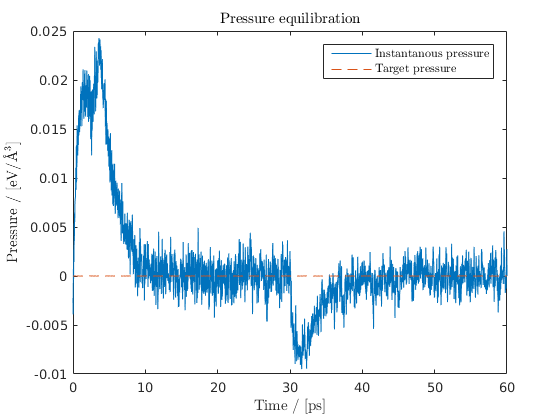
\includegraphics[width=\textwidth]{graphics/task4/pressure.png}
    \end{subfigure}
    \begin{subfigure}[b]{0.40\textwidth}
        \centering
        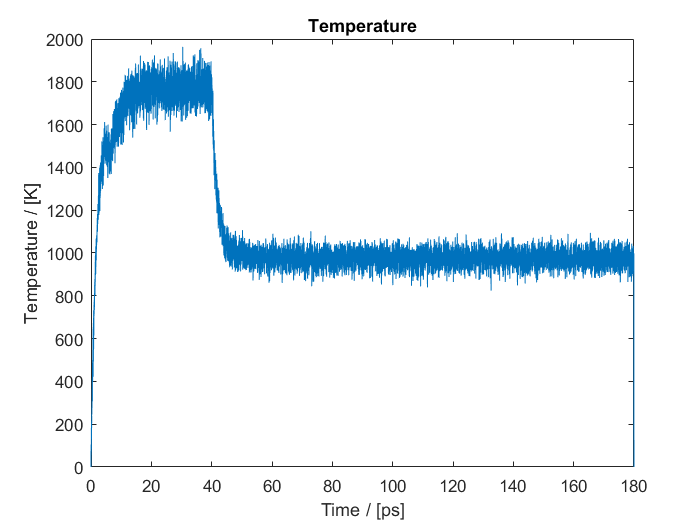
\includegraphics[width=\textwidth]{graphics/task4/temperature.png}
    \end{subfigure}
    \begin{subfigure}[b]{0.40\textwidth}
        \centering
        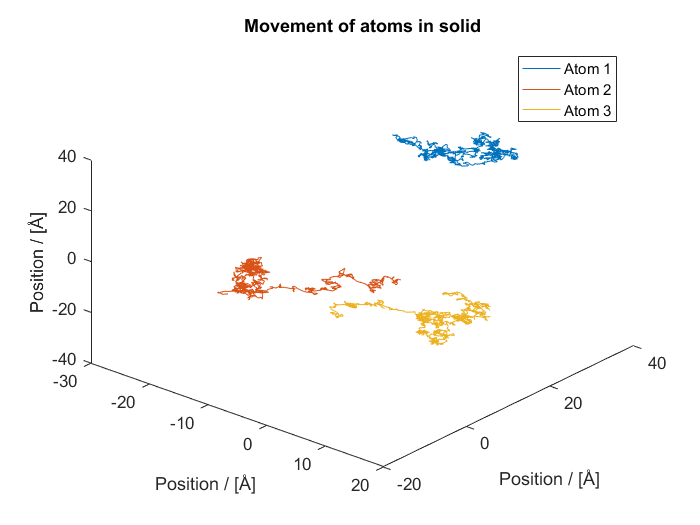
\includegraphics[width=\textwidth]{graphics/task4/traj.png}
    \end{subfigure}
    \caption{After the equilibrium, both the pressure and the temperature needs some time to stabilize after rescaling the velocities, but remains stable for longer time. The equalisation temperature was first set to $\unit[1000]{C^\circ}$ for the smelting and then the temperature was reduced to $\unit[700]{C^\circ}$.}
    \label{fig:equilibrium500}
\end{figure}


\section*{Problem 5}

$\unit[1]{\frac{j}{mol K}}=\unit[1.0366e-05]{\frac{eV}{K}}$ \\
$C_v\left[AL\right]:\unit[24.20]{\frac{j}{mol K}}=\unit[1.0366e-05]{\frac{eV}{K}}$

\noindent From our MD simulations we obtained the following values for $C_V$ when using the potential and kinetic energy fluctuations respectively.
\begin{table}[h!]
	\centering
	\caption{}
	\begin{tabular}{l|cc}
		\hline \textbf{Temperature} & \textbf{500$^\circ$ C} & \textbf{700$^\circ$ C} \\ \hline
		$C_V / (\unit{eV/kg\,K})$ (kinetic) & $5.819521 \cdot 10^{-2}$ & $5.056438 \cdot 10^{-2}$ \\
		$C_V / (\unit{eV/kg\,K})$ (potential) & $5.836188 \cdot 10^{-2}$ & $5.056541 \cdot 10^{-2}$ \\ \hline
	\end{tabular}
	\label{tab:prob5}
\end{table}

\section*{Problem 7}

\begin{figure}[H]

\end{figure}

\section*{Problem 8}


\begin{figure}[H]
    \centering
    \captionsetup[subfigure]{justification=centering}
    \begin{subfigure}[b]{0.40\textwidth}
        \centering
        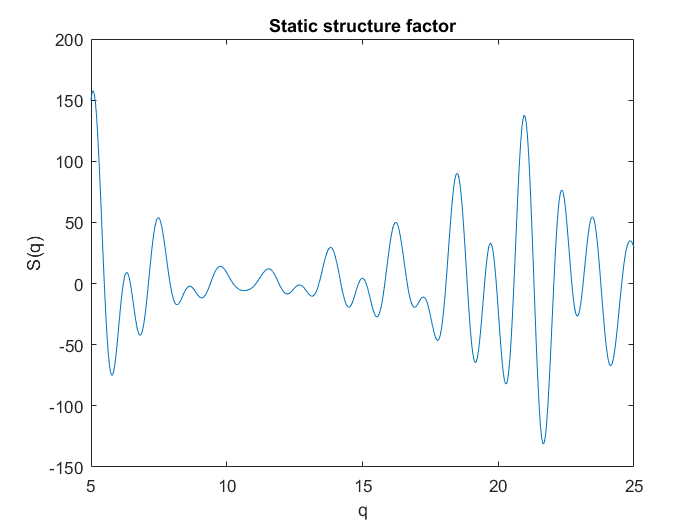
\includegraphics[width=\textwidth]{graphics/task8/integral.png}
    \end{subfigure}
    \begin{subfigure}[b]{0.40\textwidth}
        \centering
        %\resizebox{\columnwidth}{!}{% This file was created by matlab2tikz.
%
%The latest updates can be retrieved from
%  http://www.mathworks.com/matlabcentral/fileexchange/22022-matlab2tikz-matlab2tikz
%where you can also make suggestions and rate matlab2tikz.
%
\definecolor{mycolor1}{rgb}{0.00000,0.44700,0.74100}%
%
\begin{tikzpicture}

\begin{axis}[%
width=4.521in,
height=3.566in,
at={(0.758in,0.481in)},
scale only axis,
xmin=0,
xmax=1,
xlabel={Time / [$\unit{ps}$]},
ymin=800,
ymax=2000,
ylabel={Average temperature / [$\unit{\bar{K}}$]},
label style ={font=\Large},
axis background/.style={fill=white},
title style={font=\bfseries\Huge},
title={Average temperature}
]
\addplot [color=mycolor1,solid,forget plot]
  table[row sep=crcr]{%
0	973.3137\\
0	1946.575\\
0	1459.893\\
0	1297.65\\
0	1216.518\\
0.001	1167.83\\
0.001	1135.366\\
0.001	1112.172\\
0.001	1094.772\\
0.001	1081.236\\
0.001	1070.405\\
0.001	1061.541\\
0.001	1054.152\\
0.001	1047.899\\
0.001	1042.538\\
0.002	1037.892\\
0.002	1033.826\\
0.002	1030.237\\
0.002	1027.048\\
0.002	1024.194\\
0.002	1021.626\\
0.002	1019.303\\
0.002	1017.191\\
0.002	1015.264\\
0.002	1013.498\\
0.003	1011.874\\
0.003	1010.376\\
0.003	1008.989\\
0.003	1007.703\\
0.003	1006.506\\
0.003	1005.391\\
0.003	1004.348\\
0.003	1003.372\\
0.003	1002.456\\
0.003	1001.596\\
0.004	1000.786\\
0.004	1000.022\\
0.004	999.3012\\
0.004	998.6197\\
0.004	997.9746\\
0.004	997.3633\\
0.004	996.7833\\
0.004	996.2325\\
0.004	995.7089\\
0.004	995.2107\\
0.005	994.7363\\
0.005	994.2841\\
0.005	993.8529\\
0.005	993.4413\\
0.005	993.0481\\
0.005	992.6724\\
0.005	992.3131\\
0.005	991.9693\\
0.005	991.6402\\
0.005	991.3251\\
0.006	991.0231\\
0.006	990.7337\\
0.006	990.4561\\
0.006	990.1899\\
0.006	989.9344\\
0.006	989.6892\\
0.006	989.4538\\
0.006	989.2278\\
0.006	989.0106\\
0.006	988.802\\
0.007	988.6016\\
0.007	988.409\\
0.007	988.2239\\
0.007	988.046\\
0.007	987.8749\\
0.007	987.7105\\
0.007	987.5525\\
0.007	987.4005\\
0.007	987.2545\\
0.007	987.1141\\
0.008	986.9791\\
0.008	986.8495\\
0.008	986.7248\\
0.008	986.6051\\
0.008	986.4901\\
0.008	986.3796\\
0.008	986.2735\\
0.008	986.1717\\
0.008	986.0739\\
0.008	985.9801\\
0.009	985.8902\\
0.009	985.8039\\
0.009	985.7213\\
0.009	985.6421\\
0.009	985.5663\\
0.009	985.4938\\
0.009	985.4244\\
0.009	985.3581\\
0.009	985.2947\\
0.009	985.2342\\
0.009	985.1766\\
0.01	985.1216\\
0.01	985.0693\\
0.01	985.0195\\
0.01	984.9722\\
0.01	984.9274\\
0.01	984.8848\\
0.01	984.8446\\
0.01	984.8065\\
0.01	984.7706\\
0.011	984.7368\\
0.011	984.7051\\
0.011	984.6753\\
0.011	984.6474\\
0.011	984.6213\\
0.011	984.5971\\
0.011	984.5747\\
0.011	984.5539\\
0.011	984.5348\\
0.011	984.5174\\
0.011	984.5015\\
0.012	984.4871\\
0.012	984.4743\\
0.012	984.4628\\
0.012	984.4528\\
0.012	984.4442\\
0.012	984.4368\\
0.012	984.4308\\
0.012	984.426\\
0.012	984.4224\\
0.013	984.42\\
0.013	984.4188\\
0.013	984.4187\\
0.013	984.4197\\
0.013	984.4217\\
0.013	984.4247\\
0.013	984.4288\\
0.013	984.4338\\
0.013	984.4397\\
0.013	984.4466\\
0.013	984.4543\\
0.014	984.4629\\
0.014	984.4723\\
0.014	984.4825\\
0.014	984.4935\\
0.014	984.5053\\
0.014	984.5177\\
0.014	984.5309\\
0.014	984.5448\\
0.014	984.5593\\
0.015	984.5745\\
0.015	984.5902\\
0.015	984.6066\\
0.015	984.6236\\
0.015	984.6411\\
0.015	984.6591\\
0.015	984.6776\\
0.015	984.6967\\
0.015	984.7162\\
0.015	984.7362\\
0.015	984.7566\\
0.016	984.7774\\
0.016	984.7987\\
0.016	984.8203\\
0.016	984.8423\\
0.016	984.8646\\
0.016	984.8873\\
0.016	984.9104\\
0.016	984.9337\\
0.016	984.9573\\
0.017	984.9812\\
0.017	985.0054\\
0.017	985.0298\\
0.017	985.0544\\
0.017	985.0793\\
0.017	985.1044\\
0.017	985.1297\\
0.017	985.1552\\
0.017	985.1808\\
0.017	985.2066\\
0.018	985.2326\\
0.018	985.2587\\
0.018	985.2849\\
0.018	985.3113\\
0.018	985.3377\\
0.018	985.3642\\
0.018	985.3909\\
0.018	985.4176\\
0.018	985.4443\\
0.018	985.4712\\
0.019	985.498\\
0.019	985.5249\\
0.019	985.5519\\
0.019	985.5788\\
0.019	985.6058\\
0.019	985.6327\\
0.019	985.6597\\
0.019	985.6866\\
0.019	985.7136\\
0.019	985.7405\\
0.019	985.7673\\
0.02	985.7942\\
0.02	985.8209\\
0.02	985.8476\\
0.02	985.8743\\
0.02	985.9009\\
0.02	985.9274\\
0.02	985.9539\\
0.02	985.9802\\
0.02	986.0065\\
0.021	986.0326\\
0.021	986.0587\\
0.021	986.0847\\
0.021	986.1105\\
0.021	986.1363\\
0.021	986.1619\\
0.021	986.1874\\
0.021	986.2128\\
0.021	986.238\\
0.021	986.2631\\
0.022	986.2881\\
0.022	986.3129\\
0.022	986.3375\\
0.022	986.3621\\
0.022	986.3864\\
0.022	986.4106\\
0.022	986.4347\\
0.022	986.4585\\
0.022	986.4823\\
0.022	986.5058\\
0.023	986.5292\\
0.023	986.5523\\
0.023	986.5754\\
0.023	986.5982\\
0.023	986.6208\\
0.023	986.6433\\
0.023	986.6656\\
0.023	986.6876\\
0.023	986.7095\\
0.023	986.7312\\
0.024	986.7527\\
0.024	986.774\\
0.024	986.7951\\
0.024	986.816\\
0.024	986.8367\\
0.024	986.8572\\
0.024	986.8775\\
0.024	986.8976\\
0.024	986.9174\\
0.024	986.9371\\
0.025	986.9565\\
0.025	986.9757\\
0.025	986.9948\\
0.025	987.0136\\
0.025	987.0321\\
0.025	987.0505\\
0.025	987.0687\\
0.025	987.0866\\
0.025	987.1043\\
0.025	987.1218\\
0.026	987.1391\\
0.026	987.1562\\
0.026	987.173\\
0.026	987.1896\\
0.026	987.206\\
0.026	987.2222\\
0.026	987.2382\\
0.026	987.2539\\
0.026	987.2695\\
0.026	987.2848\\
0.027	987.2999\\
0.027	987.3147\\
0.027	987.3294\\
0.027	987.3439\\
0.027	987.3581\\
0.027	987.3721\\
0.027	987.3859\\
0.027	987.3995\\
0.027	987.4128\\
0.027	987.426\\
0.028	987.439\\
0.028	987.4517\\
0.028	987.4642\\
0.028	987.4765\\
0.028	987.4886\\
0.028	987.5005\\
0.028	987.5122\\
0.028	987.5237\\
0.028	987.535\\
0.028	987.5461\\
0.029	987.5569\\
0.029	987.5676\\
0.029	987.5781\\
0.029	987.5884\\
0.029	987.5984\\
0.029	987.6083\\
0.029	987.618\\
0.029	987.6275\\
0.029	987.6368\\
0.029	987.6459\\
0.03	987.6548\\
0.03	987.6636\\
0.03	987.6721\\
0.03	987.6805\\
0.03	987.6887\\
0.03	987.6967\\
0.03	987.7045\\
0.03	987.7122\\
0.03	987.7196\\
0.03	987.727\\
0.031	987.7341\\
0.031	987.7411\\
0.031	987.7479\\
0.031	987.7545\\
0.031	987.761\\
0.031	987.7674\\
0.031	987.7735\\
0.031	987.7796\\
0.031	987.7854\\
0.031	987.7912\\
0.032	987.7967\\
0.032	987.8022\\
0.032	987.8075\\
0.032	987.8126\\
0.032	987.8176\\
0.032	987.8225\\
0.032	987.8273\\
0.032	987.8319\\
0.032	987.8364\\
0.032	987.8408\\
0.033	987.8451\\
0.033	987.8492\\
0.033	987.8532\\
0.033	987.8571\\
0.033	987.8609\\
0.033	987.8646\\
0.033	987.8682\\
0.033	987.8717\\
0.033	987.8751\\
0.033	987.8784\\
0.034	987.8816\\
0.034	987.8848\\
0.034	987.8878\\
0.034	987.8908\\
0.034	987.8936\\
0.034	987.8964\\
0.034	987.8991\\
0.034	987.9018\\
0.034	987.9043\\
0.034	987.9068\\
0.035	987.9093\\
0.035	987.9116\\
0.035	987.914\\
0.035	987.9162\\
0.035	987.9184\\
0.035	987.9205\\
0.035	987.9226\\
0.035	987.9247\\
0.035	987.9267\\
0.035	987.9286\\
0.036	987.9305\\
0.036	987.9324\\
0.036	987.9342\\
0.036	987.936\\
0.036	987.9377\\
0.036	987.9394\\
0.036	987.9411\\
0.036	987.9427\\
0.036	987.9443\\
0.036	987.9459\\
0.037	987.9475\\
0.037	987.949\\
0.037	987.9505\\
0.037	987.952\\
0.037	987.9535\\
0.037	987.9549\\
0.037	987.9563\\
0.037	987.9577\\
0.037	987.9591\\
0.037	987.9605\\
0.037	987.9618\\
0.038	987.9632\\
0.038	987.9645\\
0.038	987.9658\\
0.038	987.9671\\
0.038	987.9683\\
0.038	987.9696\\
0.038	987.9708\\
0.038	987.972\\
0.038	987.9733\\
0.038	987.9744\\
0.039	987.9756\\
0.039	987.9768\\
0.039	987.9779\\
0.039	987.9791\\
0.039	987.9802\\
0.039	987.9813\\
0.039	987.9824\\
0.039	987.9835\\
0.039	987.9845\\
0.04	987.9855\\
0.04	987.9866\\
0.04	987.9875\\
0.04	987.9885\\
0.04	987.9895\\
0.04	987.9904\\
0.04	987.9913\\
0.04	987.9922\\
0.04	987.993\\
0.04	987.9939\\
0.041	987.9947\\
0.041	987.9954\\
0.041	987.9962\\
0.041	987.9969\\
0.041	987.9975\\
0.041	987.9982\\
0.041	987.9987\\
0.041	987.9993\\
0.041	987.9998\\
0.041	988.0002\\
0.042	988.0006\\
0.042	988.001\\
0.042	988.0013\\
0.042	988.0016\\
0.042	988.0018\\
0.042	988.0019\\
0.042	988.002\\
0.042	988.002\\
0.042	988.0019\\
0.042	988.0018\\
0.043	988.0016\\
0.043	988.0013\\
0.043	988.001\\
0.043	988.0005\\
0.043	988\\
0.043	987.9994\\
0.043	987.9987\\
0.043	987.998\\
0.043	987.9971\\
0.043	987.9961\\
0.044	987.995\\
0.044	987.9938\\
0.044	987.9925\\
0.044	987.9911\\
0.044	987.9896\\
0.044	987.9879\\
0.044	987.9862\\
0.044	987.9843\\
0.044	987.9822\\
0.044	987.9801\\
0.045	987.9778\\
0.045	987.9753\\
0.045	987.9727\\
0.045	987.97\\
0.045	987.9671\\
0.045	987.964\\
0.045	987.9608\\
0.045	987.9574\\
0.045	987.9539\\
0.045	987.9502\\
0.045	987.9463\\
0.046	987.9422\\
0.046	987.9379\\
0.046	987.9335\\
0.046	987.9288\\
0.046	987.924\\
0.046	987.9189\\
0.046	987.9137\\
0.046	987.9082\\
0.046	987.9026\\
0.046	987.8967\\
0.047	987.8906\\
0.047	987.8842\\
0.047	987.8777\\
0.047	987.8709\\
0.047	987.8638\\
0.047	987.8565\\
0.047	987.849\\
0.047	987.8413\\
0.047	987.8332\\
0.048	987.8249\\
0.048	987.8164\\
0.048	987.8076\\
0.048	987.7985\\
0.048	987.7891\\
0.048	987.7795\\
0.048	987.7696\\
0.048	987.7594\\
0.048	987.7489\\
0.048	987.7381\\
0.049	987.727\\
0.049	987.7157\\
0.049	987.704\\
0.049	987.692\\
0.049	987.6797\\
0.049	987.667\\
0.049	987.6541\\
0.049	987.6408\\
0.049	987.6272\\
0.049	987.6133\\
0.05	987.5991\\
0.05	987.5845\\
0.05	987.5695\\
0.05	987.5542\\
0.05	987.5386\\
0.05	987.5226\\
0.05	987.5063\\
0.05	987.4896\\
0.05	987.4726\\
0.05	987.4552\\
0.051	987.4374\\
0.051	987.4193\\
0.051	987.4008\\
0.051	987.3819\\
0.051	987.3627\\
0.051	987.3431\\
0.051	987.3231\\
0.051	987.3027\\
0.051	987.2819\\
0.051	987.2608\\
0.052	987.2392\\
0.052	987.2173\\
0.052	987.195\\
0.052	987.1723\\
0.052	987.1492\\
0.052	987.1257\\
0.052	987.1018\\
0.052	987.0775\\
0.052	987.0529\\
0.052	987.0278\\
0.053	987.0023\\
0.053	986.9764\\
0.053	986.9501\\
0.053	986.9234\\
0.053	986.8963\\
0.053	986.8688\\
0.053	986.8409\\
0.053	986.8126\\
0.053	986.7838\\
0.053	986.7547\\
0.054	986.7252\\
0.054	986.6952\\
0.054	986.6648\\
0.054	986.6341\\
0.054	986.6029\\
0.054	986.5713\\
0.054	986.5393\\
0.054	986.5069\\
0.054	986.4741\\
0.054	986.4409\\
0.054	986.4072\\
0.055	986.3732\\
0.055	986.3387\\
0.055	986.3039\\
0.055	986.2686\\
0.055	986.233\\
0.055	986.1969\\
0.055	986.1605\\
0.055	986.1236\\
0.055	986.0864\\
0.056	986.0487\\
0.056	986.0106\\
0.056	985.9722\\
0.056	985.9333\\
0.056	985.8941\\
0.056	985.8545\\
0.056	985.8145\\
0.056	985.774\\
0.056	985.7333\\
0.056	985.6921\\
0.057	985.6505\\
0.057	985.6086\\
0.057	985.5663\\
0.057	985.5236\\
0.057	985.4805\\
0.057	985.437\\
0.057	985.3932\\
0.057	985.349\\
0.057	985.3045\\
0.057	985.2596\\
0.058	985.2143\\
0.058	985.1687\\
0.058	985.1227\\
0.058	985.0764\\
0.058	985.0297\\
0.058	984.9826\\
0.058	984.9353\\
0.058	984.8875\\
0.058	984.8395\\
0.058	984.7911\\
0.059	984.7424\\
0.059	984.6933\\
0.059	984.6439\\
0.059	984.5942\\
0.059	984.5442\\
0.059	984.4938\\
0.059	984.4432\\
0.059	984.3922\\
0.059	984.341\\
0.059	984.2894\\
0.06	984.2375\\
0.06	984.1854\\
0.06	984.1329\\
0.06	984.0802\\
0.06	984.0271\\
0.06	983.9738\\
0.06	983.9202\\
0.06	983.8664\\
0.06	983.8123\\
0.06	983.7579\\
0.061	983.7032\\
0.061	983.6483\\
0.061	983.5932\\
0.061	983.5378\\
0.061	983.4821\\
0.061	983.4262\\
0.061	983.3701\\
0.061	983.3138\\
0.061	983.2572\\
0.061	983.2004\\
0.062	983.1434\\
0.062	983.0861\\
0.062	983.0287\\
0.062	982.971\\
0.062	982.9132\\
0.062	982.8551\\
0.062	982.7969\\
0.062	982.7384\\
0.062	982.6798\\
0.062	982.621\\
0.062	982.562\\
0.063	982.5029\\
0.063	982.4435\\
0.063	982.384\\
0.063	982.3244\\
0.063	982.2646\\
0.063	982.2046\\
0.063	982.1445\\
0.063	982.0843\\
0.063	982.0239\\
0.064	981.9633\\
0.064	981.9027\\
0.064	981.8419\\
0.064	981.781\\
0.064	981.72\\
0.064	981.6588\\
0.064	981.5976\\
0.064	981.5362\\
0.064	981.4748\\
0.064	981.4132\\
0.065	981.3516\\
0.065	981.2898\\
0.065	981.228\\
0.065	981.1661\\
0.065	981.1041\\
0.065	981.042\\
0.065	980.9799\\
0.065	980.9177\\
0.065	980.8555\\
0.065	980.7932\\
0.066	980.7308\\
0.066	980.6684\\
0.066	980.6059\\
0.066	980.5434\\
0.066	980.4809\\
0.066	980.4183\\
0.066	980.3557\\
0.066	980.2931\\
0.066	980.2305\\
0.066	980.1678\\
0.067	980.1052\\
0.067	980.0425\\
0.067	979.9798\\
0.067	979.9171\\
0.067	979.8544\\
0.067	979.7917\\
0.067	979.7291\\
0.067	979.6664\\
0.067	979.6038\\
0.067	979.5412\\
0.068	979.4786\\
0.068	979.4161\\
0.068	979.3536\\
0.068	979.2911\\
0.068	979.2287\\
0.068	979.1663\\
0.068	979.1039\\
0.068	979.0417\\
0.068	978.9795\\
0.068	978.9173\\
0.069	978.8552\\
0.069	978.7932\\
0.069	978.7313\\
0.069	978.6695\\
0.069	978.6077\\
0.069	978.546\\
0.069	978.4844\\
0.069	978.423\\
0.069	978.3616\\
0.069	978.3003\\
0.07	978.2392\\
0.07	978.1781\\
0.07	978.1172\\
0.07	978.0564\\
0.07	977.9957\\
0.07	977.9352\\
0.07	977.8748\\
0.07	977.8145\\
0.07	977.7544\\
0.07	977.6945\\
0.071	977.6347\\
0.071	977.575\\
0.071	977.5155\\
0.071	977.4562\\
0.071	977.3971\\
0.071	977.3381\\
0.071	977.2793\\
0.071	977.2207\\
0.071	977.1623\\
0.071	977.1041\\
0.072	977.046\\
0.072	976.9882\\
0.072	976.9306\\
0.072	976.8732\\
0.072	976.816\\
0.072	976.759\\
0.072	976.7023\\
0.072	976.6458\\
0.072	976.5895\\
0.072	976.5334\\
0.073	976.4776\\
0.073	976.4221\\
0.073	976.3668\\
0.073	976.3117\\
0.073	976.2569\\
0.073	976.2024\\
0.073	976.1481\\
0.073	976.0941\\
0.073	976.0404\\
0.073	975.987\\
0.074	975.9339\\
0.074	975.881\\
0.074	975.8285\\
0.074	975.7762\\
0.074	975.7243\\
0.074	975.6726\\
0.074	975.6213\\
0.074	975.5703\\
0.074	975.5196\\
0.074	975.4693\\
0.074	975.4193\\
0.075	975.3696\\
0.075	975.3202\\
0.075	975.2713\\
0.075	975.2226\\
0.075	975.1743\\
0.075	975.1264\\
0.075	975.0789\\
0.075	975.0317\\
0.075	974.9849\\
0.075	974.9384\\
0.076	974.8924\\
0.076	974.8467\\
0.076	974.8015\\
0.076	974.7566\\
0.076	974.7122\\
0.076	974.6681\\
0.076	974.6245\\
0.076	974.5813\\
0.076	974.5385\\
0.076	974.4962\\
0.077	974.4543\\
0.077	974.4128\\
0.077	974.3718\\
0.077	974.3312\\
0.077	974.2911\\
0.077	974.2514\\
0.077	974.2122\\
0.077	974.1735\\
0.077	974.1352\\
0.077	974.0975\\
0.078	974.0602\\
0.078	974.0234\\
0.078	973.9871\\
0.078	973.9513\\
0.078	973.916\\
0.078	973.8812\\
0.078	973.8469\\
0.078	973.8131\\
0.078	973.7799\\
0.079	973.7472\\
0.079	973.715\\
0.079	973.6834\\
0.079	973.6523\\
0.079	973.6217\\
0.079	973.5917\\
0.079	973.5623\\
0.079	973.5334\\
0.079	973.5051\\
0.079	973.4773\\
0.08	973.4501\\
0.08	973.4235\\
0.08	973.3975\\
0.08	973.3721\\
0.08	973.3472\\
0.08	973.3229\\
0.08	973.2993\\
0.08	973.2762\\
0.08	973.2538\\
0.08	973.2319\\
0.081	973.2106\\
0.081	973.19\\
0.081	973.17\\
0.081	973.1506\\
0.081	973.1318\\
0.081	973.1137\\
0.081	973.0962\\
0.081	973.0793\\
0.081	973.0631\\
0.081	973.0475\\
0.082	973.0325\\
0.082	973.0182\\
0.082	973.0046\\
0.082	972.9916\\
0.082	972.9792\\
0.082	972.9675\\
0.082	972.9565\\
0.082	972.9462\\
0.082	972.9364\\
0.082	972.9274\\
0.083	972.919\\
0.083	972.9114\\
0.083	972.9043\\
0.083	972.898\\
0.083	972.8923\\
0.083	972.8873\\
0.083	972.883\\
0.083	972.8794\\
0.083	972.8765\\
0.083	972.8742\\
0.084	972.8726\\
0.084	972.8717\\
0.084	972.8716\\
0.084	972.8721\\
0.084	972.8732\\
0.084	972.8751\\
0.084	972.8777\\
0.084	972.881\\
0.084	972.8849\\
0.084	972.8896\\
0.085	972.895\\
0.085	972.901\\
0.085	972.9078\\
0.085	972.9152\\
0.085	972.9233\\
0.085	972.9322\\
0.085	972.9417\\
0.085	972.9519\\
0.085	972.9629\\
0.085	972.9745\\
0.086	972.9868\\
0.086	972.9998\\
0.086	973.0135\\
0.086	973.0279\\
0.086	973.043\\
0.086	973.0587\\
0.086	973.0752\\
0.086	973.0924\\
0.086	973.1102\\
0.086	973.1287\\
0.087	973.1479\\
0.087	973.1678\\
0.087	973.1884\\
0.087	973.2096\\
0.087	973.2315\\
0.087	973.2541\\
0.087	973.2774\\
0.087	973.3013\\
0.087	973.3259\\
0.087	973.3511\\
0.088	973.377\\
0.088	973.4036\\
0.088	973.4308\\
0.088	973.4587\\
0.088	973.4872\\
0.088	973.5164\\
0.088	973.5462\\
0.088	973.5767\\
0.088	973.6078\\
0.088	973.6395\\
0.089	973.6718\\
0.089	973.7048\\
0.089	973.7384\\
0.089	973.7726\\
0.089	973.8074\\
0.089	973.8428\\
0.089	973.8788\\
0.089	973.9154\\
0.089	973.9526\\
0.089	973.9904\\
0.09	974.0287\\
0.09	974.0677\\
0.09	974.1072\\
0.09	974.1472\\
0.09	974.1879\\
0.09	974.229\\
0.09	974.2708\\
0.09	974.313\\
0.09	974.3558\\
0.09	974.3992\\
0.091	974.443\\
0.091	974.4874\\
0.091	974.5323\\
0.091	974.5777\\
0.091	974.6236\\
0.091	974.6699\\
0.091	974.7168\\
0.091	974.7641\\
0.091	974.8119\\
0.091	974.8602\\
0.091	974.9089\\
0.092	974.9581\\
0.092	975.0077\\
0.092	975.0577\\
0.092	975.1081\\
0.092	975.159\\
0.092	975.2103\\
0.092	975.262\\
0.092	975.314\\
0.092	975.3665\\
0.092	975.4193\\
0.093	975.4725\\
0.093	975.526\\
0.093	975.5799\\
0.093	975.6342\\
0.093	975.6887\\
0.093	975.7436\\
0.093	975.7988\\
0.093	975.8543\\
0.093	975.9101\\
0.093	975.9662\\
0.094	976.0226\\
0.094	976.0792\\
0.094	976.1361\\
0.094	976.1932\\
0.094	976.2506\\
0.094	976.3082\\
0.094	976.366\\
0.094	976.424\\
0.094	976.4822\\
0.095	976.5406\\
0.095	976.5992\\
0.095	976.658\\
0.095	976.7169\\
0.095	976.7759\\
0.095	976.8351\\
0.095	976.8944\\
0.095	976.9539\\
0.095	977.0134\\
0.095	977.073\\
0.096	977.1327\\
0.096	977.1925\\
0.096	977.2524\\
0.096	977.3123\\
0.096	977.3722\\
0.096	977.4322\\
0.096	977.4922\\
0.096	977.5522\\
0.096	977.6122\\
0.096	977.6722\\
0.097	977.7322\\
0.097	977.7921\\
0.097	977.852\\
0.097	977.9118\\
0.097	977.9716\\
0.097	978.0313\\
0.097	978.0909\\
0.097	978.1504\\
0.097	978.2098\\
0.097	978.269\\
0.098	978.3281\\
0.098	978.3871\\
0.098	978.446\\
0.098	978.5046\\
0.098	978.5631\\
0.098	978.6214\\
0.098	978.6795\\
0.098	978.7374\\
0.098	978.795\\
0.098	978.8525\\
0.099	978.9096\\
0.099	978.9666\\
0.099	979.0232\\
0.099	979.0796\\
0.099	979.1357\\
0.099	979.1915\\
0.099	979.247\\
0.099	979.3022\\
0.099	979.3571\\
0.099	979.4116\\
0.1	979.4657\\
0.1	979.5195\\
0.1	979.5729\\
0.1	979.626\\
0.1	979.6786\\
0.1	979.7309\\
0.1	979.7827\\
0.1	979.8341\\
0.1	979.885\\
0.1	979.9356\\
0.101	979.9856\\
0.101	980.0352\\
0.101	980.0844\\
0.101	980.133\\
0.101	980.1811\\
0.101	980.2288\\
0.101	980.2759\\
0.101	980.3225\\
0.101	980.3685\\
0.101	980.4141\\
0.102	980.459\\
0.102	980.5034\\
0.102	980.5473\\
0.102	980.5905\\
0.102	980.6332\\
0.102	980.6752\\
0.102	980.7167\\
0.102	980.7575\\
0.102	980.7977\\
0.102	980.8373\\
0.103	980.8762\\
0.103	980.9145\\
0.103	980.9521\\
0.103	980.9891\\
0.103	981.0253\\
0.103	981.0609\\
0.103	981.0958\\
0.103	981.13\\
0.103	981.1635\\
0.103	981.1963\\
0.104	981.2283\\
0.104	981.2596\\
0.104	981.2902\\
0.104	981.32\\
0.104	981.3491\\
0.104	981.3774\\
0.104	981.405\\
0.104	981.4318\\
0.104	981.4578\\
0.104	981.483\\
0.105	981.5075\\
0.105	981.5311\\
0.105	981.554\\
0.105	981.576\\
0.105	981.5972\\
0.105	981.6176\\
0.105	981.6372\\
0.105	981.656\\
0.105	981.6739\\
0.105	981.691\\
0.106	981.7072\\
0.106	981.7226\\
0.106	981.7371\\
0.106	981.7508\\
0.106	981.7636\\
0.106	981.7756\\
0.106	981.7867\\
0.106	981.7969\\
0.106	981.8063\\
0.106	981.8148\\
0.107	981.8224\\
0.107	981.8291\\
0.107	981.8349\\
0.107	981.8399\\
0.107	981.8439\\
0.107	981.8471\\
0.107	981.8494\\
0.107	981.8508\\
0.107	981.8512\\
0.107	981.8508\\
0.107	981.8495\\
0.108	981.8473\\
0.108	981.8442\\
0.108	981.8402\\
0.108	981.8353\\
0.108	981.8294\\
0.108	981.8227\\
0.108	981.8151\\
0.108	981.8066\\
0.108	981.7971\\
0.108	981.7868\\
0.109	981.7756\\
0.109	981.7635\\
0.109	981.7504\\
0.109	981.7365\\
0.109	981.7217\\
0.109	981.7059\\
0.109	981.6893\\
0.109	981.6718\\
0.109	981.6534\\
0.11	981.6342\\
0.11	981.614\\
0.11	981.593\\
0.11	981.571\\
0.11	981.5482\\
0.11	981.5246\\
0.11	981.5\\
0.11	981.4746\\
0.11	981.4484\\
0.11	981.4212\\
0.111	981.3933\\
0.111	981.3644\\
0.111	981.3348\\
0.111	981.3042\\
0.111	981.2729\\
0.111	981.2407\\
0.111	981.2077\\
0.111	981.1739\\
0.111	981.1392\\
0.111	981.1038\\
0.112	981.0675\\
0.112	981.0305\\
0.112	980.9926\\
0.112	980.954\\
0.112	980.9146\\
0.112	980.8744\\
0.112	980.8334\\
0.112	980.7917\\
0.112	980.7493\\
0.112	980.706\\
0.113	980.6621\\
0.113	980.6174\\
0.113	980.572\\
0.113	980.5259\\
0.113	980.4791\\
0.113	980.4315\\
0.113	980.3833\\
0.113	980.3344\\
0.113	980.2848\\
0.113	980.2345\\
0.114	980.1836\\
0.114	980.1321\\
0.114	980.0798\\
0.114	980.027\\
0.114	979.9735\\
0.114	979.9194\\
0.114	979.8648\\
0.114	979.8095\\
0.114	979.7536\\
0.114	979.6971\\
0.115	979.6401\\
0.115	979.5825\\
0.115	979.5244\\
0.115	979.4657\\
0.115	979.4065\\
0.115	979.3468\\
0.115	979.2865\\
0.115	979.2258\\
0.115	979.1646\\
0.115	979.1029\\
0.116	979.0407\\
0.116	978.978\\
0.116	978.915\\
0.116	978.8514\\
0.116	978.7875\\
0.116	978.7231\\
0.116	978.6583\\
0.116	978.5932\\
0.116	978.5276\\
0.116	978.4617\\
0.117	978.3954\\
0.117	978.3288\\
0.117	978.2618\\
0.117	978.1945\\
0.117	978.1268\\
0.117	978.0589\\
0.117	977.9907\\
0.117	977.9221\\
0.117	977.8533\\
0.117	977.7843\\
0.118	977.715\\
0.118	977.6454\\
0.118	977.5756\\
0.118	977.5056\\
0.118	977.4354\\
0.118	977.365\\
0.118	977.2944\\
0.118	977.2236\\
0.118	977.1527\\
0.118	977.0816\\
0.119	977.0103\\
0.119	976.9389\\
0.119	976.8674\\
0.119	976.7958\\
0.119	976.7241\\
0.119	976.6523\\
0.119	976.5804\\
0.119	976.5085\\
0.119	976.4365\\
0.119	976.3644\\
0.12	976.2924\\
0.12	976.2202\\
0.12	976.1481\\
0.12	976.076\\
0.12	976.0038\\
0.12	975.9317\\
0.12	975.8596\\
0.12	975.7876\\
0.12	975.7156\\
0.12	975.6436\\
0.121	975.5717\\
0.121	975.4999\\
0.121	975.4282\\
0.121	975.3565\\
0.121	975.285\\
0.121	975.2136\\
0.121	975.1422\\
0.121	975.0711\\
0.121	975\\
0.121	974.9291\\
0.122	974.8584\\
0.122	974.7878\\
0.122	974.7175\\
0.122	974.6472\\
0.122	974.5772\\
0.122	974.5074\\
0.122	974.4378\\
0.122	974.3684\\
0.122	974.2992\\
0.122	974.2303\\
0.123	974.1616\\
0.123	974.0932\\
0.123	974.025\\
0.123	973.957\\
0.123	973.8894\\
0.123	973.822\\
0.123	973.7549\\
0.123	973.6881\\
0.123	973.6215\\
0.123	973.5553\\
0.124	973.4894\\
0.124	973.4238\\
0.124	973.3586\\
0.124	973.2936\\
0.124	973.229\\
0.124	973.1648\\
0.124	973.1008\\
0.124	973.0373\\
0.124	972.9741\\
0.124	972.9112\\
0.124	972.8488\\
0.125	972.7866\\
0.125	972.7249\\
0.125	972.6636\\
0.125	972.6026\\
0.125	972.542\\
0.125	972.4819\\
0.125	972.4221\\
0.125	972.3627\\
0.125	972.3038\\
0.126	972.2452\\
0.126	972.1871\\
0.126	972.1294\\
0.126	972.0721\\
0.126	972.0152\\
0.126	971.9588\\
0.126	971.9028\\
0.126	971.8472\\
0.126	971.7921\\
0.126	971.7374\\
0.127	971.6831\\
0.127	971.6293\\
0.127	971.576\\
0.127	971.5231\\
0.127	971.4706\\
0.127	971.4186\\
0.127	971.3671\\
0.127	971.316\\
0.127	971.2654\\
0.127	971.2152\\
0.128	971.1655\\
0.128	971.1163\\
0.128	971.0675\\
0.128	971.0191\\
0.128	970.9713\\
0.128	970.9239\\
0.128	970.877\\
0.128	970.8305\\
0.128	970.7845\\
0.128	970.739\\
0.129	970.6939\\
0.129	970.6493\\
0.129	970.6052\\
0.129	970.5615\\
0.129	970.5183\\
0.129	970.4756\\
0.129	970.4333\\
0.129	970.3915\\
0.129	970.3502\\
0.129	970.3093\\
0.13	970.2688\\
0.13	970.2289\\
0.13	970.1893\\
0.13	970.1503\\
0.13	970.1117\\
0.13	970.0735\\
0.13	970.0358\\
0.13	969.9985\\
0.13	969.9617\\
0.13	969.9254\\
0.131	969.8894\\
0.131	969.854\\
0.131	969.8189\\
0.131	969.7843\\
0.131	969.7501\\
0.131	969.7164\\
0.131	969.6831\\
0.131	969.6502\\
0.131	969.6177\\
0.131	969.5857\\
0.132	969.554\\
0.132	969.5228\\
0.132	969.492\\
0.132	969.4616\\
0.132	969.4317\\
0.132	969.4021\\
0.132	969.3729\\
0.132	969.3441\\
0.132	969.3157\\
0.132	969.2878\\
0.133	969.2601\\
0.133	969.2329\\
0.133	969.2061\\
0.133	969.1796\\
0.133	969.1535\\
0.133	969.1278\\
0.133	969.1025\\
0.133	969.0775\\
0.133	969.0529\\
0.133	969.0286\\
0.134	969.0047\\
0.134	968.9811\\
0.134	968.9579\\
0.134	968.935\\
0.134	968.9125\\
0.134	968.8903\\
0.134	968.8684\\
0.134	968.8469\\
0.134	968.8256\\
0.134	968.8047\\
0.135	968.7841\\
0.135	968.7638\\
0.135	968.7439\\
0.135	968.7242\\
0.135	968.7048\\
0.135	968.6858\\
0.135	968.667\\
0.135	968.6485\\
0.135	968.6303\\
0.135	968.6123\\
0.136	968.5947\\
0.136	968.5773\\
0.136	968.5602\\
0.136	968.5433\\
0.136	968.5267\\
0.136	968.5104\\
0.136	968.4943\\
0.136	968.4784\\
0.136	968.4628\\
0.136	968.4475\\
0.137	968.4324\\
0.137	968.4175\\
0.137	968.4028\\
0.137	968.3884\\
0.137	968.3742\\
0.137	968.3602\\
0.137	968.3464\\
0.137	968.3328\\
0.137	968.3195\\
0.137	968.3063\\
0.138	968.2934\\
0.138	968.2806\\
0.138	968.268\\
0.138	968.2557\\
0.138	968.2435\\
0.138	968.2314\\
0.138	968.2196\\
0.138	968.2079\\
0.138	968.1964\\
0.138	968.1851\\
0.139	968.174\\
0.139	968.163\\
0.139	968.1521\\
0.139	968.1415\\
0.139	968.1309\\
0.139	968.1206\\
0.139	968.1103\\
0.139	968.1003\\
0.139	968.0903\\
0.139	968.0805\\
0.14	968.0709\\
0.14	968.0613\\
0.14	968.0519\\
0.14	968.0427\\
0.14	968.0335\\
0.14	968.0245\\
0.14	968.0156\\
0.14	968.0068\\
0.14	967.9982\\
0.14	967.9896\\
0.141	967.9812\\
0.141	967.9729\\
0.141	967.9647\\
0.141	967.9566\\
0.141	967.9486\\
0.141	967.9407\\
0.141	967.9329\\
0.141	967.9252\\
0.141	967.9176\\
0.141	967.9101\\
0.142	967.9028\\
0.142	967.8955\\
0.142	967.8882\\
0.142	967.8811\\
0.142	967.8741\\
0.142	967.8672\\
0.142	967.8603\\
0.142	967.8536\\
0.142	967.8469\\
0.142	967.8403\\
0.143	967.8338\\
0.143	967.8274\\
0.143	967.8211\\
0.143	967.8148\\
0.143	967.8087\\
0.143	967.8026\\
0.143	967.7966\\
0.143	967.7907\\
0.143	967.7848\\
0.143	967.7791\\
0.144	967.7734\\
0.144	967.7678\\
0.144	967.7623\\
0.144	967.7568\\
0.144	967.7515\\
0.144	967.7462\\
0.144	967.741\\
0.144	967.7359\\
0.144	967.7308\\
0.144	967.7259\\
0.145	967.721\\
0.145	967.7162\\
0.145	967.7114\\
0.145	967.7068\\
0.145	967.7023\\
0.145	967.6978\\
0.145	967.6934\\
0.145	967.6891\\
0.145	967.6849\\
0.145	967.6807\\
0.146	967.6767\\
0.146	967.6727\\
0.146	967.6688\\
0.146	967.665\\
0.146	967.6613\\
0.146	967.6577\\
0.146	967.6542\\
0.146	967.6508\\
0.146	967.6475\\
0.146	967.6442\\
0.147	967.6411\\
0.147	967.638\\
0.147	967.6351\\
0.147	967.6322\\
0.147	967.6295\\
0.147	967.6268\\
0.147	967.6243\\
0.147	967.6219\\
0.147	967.6195\\
0.147	967.6173\\
0.148	967.6152\\
0.148	967.6132\\
0.148	967.6113\\
0.148	967.6095\\
0.148	967.6079\\
0.148	967.6063\\
0.148	967.6049\\
0.148	967.6036\\
0.148	967.6024\\
0.148	967.6014\\
0.149	967.6004\\
0.149	967.5996\\
0.149	967.5989\\
0.149	967.5984\\
0.149	967.5979\\
0.149	967.5977\\
0.149	967.5975\\
0.149	967.5975\\
0.149	967.5976\\
0.149	967.5979\\
0.149	967.5983\\
0.15	967.5988\\
0.15	967.5995\\
0.15	967.6003\\
0.15	967.6013\\
0.15	967.6024\\
0.15	967.6037\\
0.15	967.6051\\
0.15	967.6067\\
0.15	967.6084\\
0.15	967.6103\\
0.151	967.6123\\
0.151	967.6145\\
0.151	967.6169\\
0.151	967.6194\\
0.151	967.6221\\
0.151	967.6249\\
0.151	967.6279\\
0.151	967.6311\\
0.151	967.6344\\
0.151	967.6379\\
0.152	967.6416\\
0.152	967.6454\\
0.152	967.6495\\
0.152	967.6537\\
0.152	967.658\\
0.152	967.6626\\
0.152	967.6673\\
0.152	967.6722\\
0.152	967.6773\\
0.152	967.6825\\
0.153	967.6879\\
0.153	967.6936\\
0.153	967.6994\\
0.153	967.7053\\
0.153	967.7115\\
0.153	967.7179\\
0.153	967.7244\\
0.153	967.7311\\
0.153	967.738\\
0.153	967.7451\\
0.154	967.7524\\
0.154	967.7599\\
0.154	967.7676\\
0.154	967.7754\\
0.154	967.7835\\
0.154	967.7917\\
0.154	967.8002\\
0.154	967.8088\\
0.154	967.8176\\
0.154	967.8266\\
0.155	967.8359\\
0.155	967.8453\\
0.155	967.8549\\
0.155	967.8647\\
0.155	967.8747\\
0.155	967.8848\\
0.155	967.8952\\
0.155	967.9058\\
0.155	967.9166\\
0.155	967.9276\\
0.156	967.9387\\
0.156	967.9501\\
0.156	967.9617\\
0.156	967.9734\\
0.156	967.9854\\
0.156	967.9976\\
0.156	968.0099\\
0.156	968.0225\\
0.156	968.0352\\
0.157	968.0481\\
0.157	968.0613\\
0.157	968.0746\\
0.157	968.0881\\
0.157	968.1018\\
0.157	968.1158\\
0.157	968.1299\\
0.157	968.1442\\
0.157	968.1586\\
0.157	968.1733\\
0.158	968.1882\\
0.158	968.2033\\
0.158	968.2185\\
0.158	968.234\\
0.158	968.2496\\
0.158	968.2654\\
0.158	968.2814\\
0.158	968.2976\\
0.158	968.314\\
0.158	968.3306\\
0.159	968.3473\\
0.159	968.3643\\
0.159	968.3814\\
0.159	968.3987\\
0.159	968.4161\\
0.159	968.4338\\
0.159	968.4516\\
0.159	968.4696\\
0.159	968.4878\\
0.159	968.5062\\
0.16	968.5247\\
0.16	968.5434\\
0.16	968.5623\\
0.16	968.5813\\
0.16	968.6005\\
0.16	968.6199\\
0.16	968.6395\\
0.16	968.6592\\
0.16	968.6791\\
0.16	968.6991\\
0.161	968.7193\\
0.161	968.7396\\
0.161	968.7602\\
0.161	968.7808\\
0.161	968.8016\\
0.161	968.8226\\
0.161	968.8437\\
0.161	968.865\\
0.161	968.8864\\
0.161	968.908\\
0.162	968.9297\\
0.162	968.9516\\
0.162	968.9735\\
0.162	968.9957\\
0.162	969.0179\\
0.162	969.0403\\
0.162	969.0629\\
0.162	969.0855\\
0.162	969.1083\\
0.162	969.1313\\
0.163	969.1543\\
0.163	969.1775\\
0.163	969.2008\\
0.163	969.2242\\
0.163	969.2477\\
0.163	969.2714\\
0.163	969.2951\\
0.163	969.319\\
0.163	969.343\\
0.163	969.367\\
0.164	969.3912\\
0.164	969.4155\\
0.164	969.4399\\
0.164	969.4644\\
0.164	969.489\\
0.164	969.5137\\
0.164	969.5384\\
0.164	969.5633\\
0.164	969.5882\\
0.164	969.6133\\
0.165	969.6384\\
0.165	969.6636\\
0.165	969.6889\\
0.165	969.7142\\
0.165	969.7396\\
0.165	969.7651\\
0.165	969.7907\\
0.165	969.8163\\
0.165	969.842\\
0.165	969.8678\\
0.166	969.8936\\
0.166	969.9195\\
0.166	969.9455\\
0.166	969.9714\\
0.166	969.9975\\
0.166	970.0236\\
0.166	970.0497\\
0.166	970.0759\\
0.166	970.1021\\
0.166	970.1284\\
0.167	970.1547\\
0.167	970.1811\\
0.167	970.2074\\
0.167	970.2339\\
0.167	970.2603\\
0.167	970.2868\\
0.167	970.3133\\
0.167	970.3398\\
0.167	970.3663\\
0.167	970.3929\\
0.168	970.4194\\
0.168	970.446\\
0.168	970.4726\\
0.168	970.4992\\
0.168	970.5258\\
0.168	970.5524\\
0.168	970.5791\\
0.168	970.6057\\
0.168	970.6323\\
0.168	970.6589\\
0.169	970.6855\\
0.169	970.7122\\
0.169	970.7387\\
0.169	970.7653\\
0.169	970.7919\\
0.169	970.8185\\
0.169	970.845\\
0.169	970.8715\\
0.169	970.898\\
0.169	970.9245\\
0.17	970.9509\\
0.17	970.9773\\
0.17	971.0037\\
0.17	971.0301\\
0.17	971.0564\\
0.17	971.0827\\
0.17	971.1089\\
0.17	971.1351\\
0.17	971.1613\\
0.17	971.1874\\
0.171	971.2134\\
0.171	971.2395\\
0.171	971.2654\\
0.171	971.2913\\
0.171	971.3172\\
0.171	971.343\\
0.171	971.3687\\
0.171	971.3944\\
0.171	971.4201\\
0.171	971.4456\\
0.172	971.4711\\
0.172	971.4965\\
0.172	971.5219\\
0.172	971.5472\\
0.172	971.5724\\
0.172	971.5975\\
0.172	971.6226\\
0.172	971.6476\\
0.172	971.6725\\
0.172	971.6973\\
0.173	971.722\\
0.173	971.7467\\
0.173	971.7712\\
0.173	971.7957\\
0.173	971.8201\\
0.173	971.8444\\
0.173	971.8686\\
0.173	971.8927\\
0.173	971.9167\\
0.173	971.9406\\
0.174	971.9644\\
0.174	971.9882\\
0.174	972.0118\\
0.174	972.0353\\
0.174	972.0587\\
0.174	972.082\\
0.174	972.1051\\
0.174	972.1282\\
0.174	972.1512\\
0.174	972.174\\
0.175	972.1968\\
0.175	972.2194\\
0.175	972.2419\\
0.175	972.2643\\
0.175	972.2866\\
0.175	972.3087\\
0.175	972.3308\\
0.175	972.3527\\
0.175	972.3745\\
0.175	972.3961\\
0.176	972.4177\\
0.176	972.4391\\
0.176	972.4604\\
0.176	972.4815\\
0.176	972.5025\\
0.176	972.5234\\
0.176	972.5442\\
0.176	972.5648\\
0.176	972.5853\\
0.176	972.6057\\
0.177	972.6259\\
0.177	972.646\\
0.177	972.6659\\
0.177	972.6857\\
0.177	972.7054\\
0.177	972.7249\\
0.177	972.7443\\
0.177	972.7635\\
0.177	972.7826\\
0.177	972.8015\\
0.178	972.8203\\
0.178	972.839\\
0.178	972.8575\\
0.178	972.8758\\
0.178	972.8941\\
0.178	972.9121\\
0.178	972.93\\
0.178	972.9478\\
0.178	972.9654\\
0.178	972.9828\\
0.179	973.0001\\
0.179	973.0173\\
0.179	973.0342\\
0.179	973.0511\\
0.179	973.0677\\
0.179	973.0842\\
0.179	973.1006\\
0.179	973.1168\\
0.179	973.1328\\
0.179	973.1487\\
0.18	973.1644\\
0.18	973.1799\\
0.18	973.1953\\
0.18	973.2105\\
0.18	973.2256\\
0.18	973.2405\\
0.18	973.2552\\
0.18	973.2698\\
0.18	973.2842\\
0.18	973.2984\\
0.181	973.3124\\
0.181	973.3263\\
0.181	973.34\\
0.181	973.3536\\
0.181	973.3669\\
0.181	973.3801\\
0.181	973.3932\\
0.181	973.406\\
0.181	973.4187\\
0.181	973.4312\\
0.182	973.4435\\
0.182	973.4557\\
0.182	973.4677\\
0.182	973.4795\\
0.182	973.4911\\
0.182	973.5025\\
0.182	973.5138\\
0.182	973.5249\\
0.182	973.5358\\
0.182	973.5465\\
0.182	973.5571\\
0.183	973.5674\\
0.183	973.5776\\
0.183	973.5876\\
0.183	973.5974\\
0.183	973.6071\\
0.183	973.6165\\
0.183	973.6258\\
0.183	973.6348\\
0.183	973.6437\\
0.183	973.6524\\
0.184	973.661\\
0.184	973.6693\\
0.184	973.6774\\
0.184	973.6854\\
0.184	973.6931\\
0.184	973.7007\\
0.184	973.7081\\
0.184	973.7153\\
0.184	973.7222\\
0.184	973.729\\
0.185	973.7356\\
0.185	973.742\\
0.185	973.7483\\
0.185	973.7543\\
0.185	973.7601\\
0.185	973.7657\\
0.185	973.7711\\
0.185	973.7764\\
0.185	973.7814\\
0.185	973.7862\\
0.186	973.7909\\
0.186	973.7953\\
0.186	973.7995\\
0.186	973.8035\\
0.186	973.8073\\
0.186	973.811\\
0.186	973.8144\\
0.186	973.8176\\
0.186	973.8206\\
0.186	973.8234\\
0.187	973.8259\\
0.187	973.8283\\
0.187	973.8305\\
0.187	973.8324\\
0.187	973.8342\\
0.187	973.8357\\
0.187	973.8371\\
0.187	973.8382\\
0.187	973.8391\\
0.188	973.8398\\
0.188	973.8402\\
0.188	973.8405\\
0.188	973.8405\\
0.188	973.8404\\
0.188	973.84\\
0.188	973.8393\\
0.188	973.8385\\
0.188	973.8375\\
0.188	973.8362\\
0.189	973.8347\\
0.189	973.833\\
0.189	973.8311\\
0.189	973.8289\\
0.189	973.8266\\
0.189	973.824\\
0.189	973.8211\\
0.189	973.8181\\
0.189	973.8148\\
0.189	973.8113\\
0.19	973.8076\\
0.19	973.8037\\
0.19	973.7995\\
0.19	973.7951\\
0.19	973.7905\\
0.19	973.7856\\
0.19	973.7806\\
0.19	973.7753\\
0.19	973.7697\\
0.19	973.7639\\
0.191	973.758\\
0.191	973.7517\\
0.191	973.7453\\
0.191	973.7386\\
0.191	973.7317\\
0.191	973.7245\\
0.191	973.7172\\
0.191	973.7095\\
0.191	973.7017\\
0.191	973.6936\\
0.192	973.6853\\
0.192	973.6768\\
0.192	973.668\\
0.192	973.659\\
0.192	973.6498\\
0.192	973.6404\\
0.192	973.6307\\
0.192	973.6208\\
0.192	973.6106\\
0.192	973.6002\\
0.193	973.5896\\
0.193	973.5788\\
0.193	973.5677\\
0.193	973.5564\\
0.193	973.5449\\
0.193	973.5331\\
0.193	973.5212\\
0.193	973.5089\\
0.193	973.4965\\
0.193	973.4838\\
0.194	973.471\\
0.194	973.4578\\
0.194	973.4445\\
0.194	973.4309\\
0.194	973.4172\\
0.194	973.4032\\
0.194	973.3889\\
0.194	973.3745\\
0.194	973.3598\\
0.194	973.3449\\
0.195	973.3298\\
0.195	973.3145\\
0.195	973.299\\
0.195	973.2832\\
0.195	973.2673\\
0.195	973.2511\\
0.195	973.2347\\
0.195	973.2181\\
0.195	973.2013\\
0.195	973.1843\\
0.196	973.1671\\
0.196	973.1496\\
0.196	973.132\\
0.196	973.1142\\
0.196	973.0962\\
0.196	973.0779\\
0.196	973.0595\\
0.196	973.0409\\
0.196	973.0221\\
0.196	973.0031\\
0.197	972.9839\\
0.197	972.9645\\
0.197	972.9449\\
0.197	972.9251\\
0.197	972.9052\\
0.197	972.885\\
0.197	972.8647\\
0.197	972.8442\\
0.197	972.8236\\
0.197	972.8027\\
0.198	972.7817\\
0.198	972.7605\\
0.198	972.7392\\
0.198	972.7177\\
0.198	972.696\\
0.198	972.6741\\
0.198	972.6521\\
0.198	972.63\\
0.198	972.6076\\
0.198	972.5852\\
0.199	972.5625\\
0.199	972.5398\\
0.199	972.5168\\
0.199	972.4938\\
0.199	972.4706\\
0.199	972.4472\\
0.199	972.4237\\
0.199	972.4001\\
0.199	972.3764\\
0.199	972.3525\\
0.2	972.3285\\
0.2	972.3043\\
0.2	972.2801\\
0.2	972.2557\\
0.2	972.2312\\
0.2	972.2066\\
0.2	972.1819\\
0.2	972.1571\\
0.2	972.1322\\
0.2	972.1072\\
0.201	972.082\\
0.201	972.0568\\
0.201	972.0315\\
0.201	972.0061\\
0.201	971.9806\\
0.201	971.955\\
0.201	971.9293\\
0.201	971.9036\\
0.201	971.8778\\
0.201	971.8519\\
0.202	971.8259\\
0.202	971.7999\\
0.202	971.7738\\
0.202	971.7476\\
0.202	971.7214\\
0.202	971.6951\\
0.202	971.6688\\
0.202	971.6424\\
0.202	971.6159\\
0.202	971.5895\\
0.203	971.563\\
0.203	971.5364\\
0.203	971.5098\\
0.203	971.4832\\
0.203	971.4566\\
0.203	971.4299\\
0.203	971.4032\\
0.203	971.3765\\
0.203	971.3498\\
0.203	971.323\\
0.204	971.2963\\
0.204	971.2695\\
0.204	971.2427\\
0.204	971.216\\
0.204	971.1892\\
0.204	971.1625\\
0.204	971.1357\\
0.204	971.109\\
0.204	971.0823\\
0.204	971.0556\\
0.205	971.0289\\
0.205	971.0022\\
0.205	970.9756\\
0.205	970.949\\
0.205	970.9225\\
0.205	970.8959\\
0.205	970.8695\\
0.205	970.843\\
0.205	970.8166\\
0.205	970.7903\\
0.206	970.764\\
0.206	970.7377\\
0.206	970.7115\\
0.206	970.6854\\
0.206	970.6594\\
0.206	970.6334\\
0.206	970.6074\\
0.206	970.5816\\
0.206	970.5558\\
0.206	970.5301\\
0.207	970.5045\\
0.207	970.479\\
0.207	970.4535\\
0.207	970.4281\\
0.207	970.4029\\
0.207	970.3777\\
0.207	970.3526\\
0.207	970.3276\\
0.207	970.3028\\
0.207	970.278\\
0.208	970.2533\\
0.208	970.2288\\
0.208	970.2043\\
0.208	970.18\\
0.208	970.1558\\
0.208	970.1317\\
0.208	970.1078\\
0.208	970.0839\\
0.208	970.0602\\
0.208	970.0366\\
0.209	970.0132\\
0.209	969.9899\\
0.209	969.9667\\
0.209	969.9436\\
0.209	969.9207\\
0.209	969.898\\
0.209	969.8754\\
0.209	969.8529\\
0.209	969.8306\\
0.209	969.8084\\
0.21	969.7864\\
0.21	969.7646\\
0.21	969.7429\\
0.21	969.7213\\
0.21	969.7\\
0.21	969.6787\\
0.21	969.6577\\
0.21	969.6368\\
0.21	969.6161\\
0.21	969.5955\\
0.211	969.5752\\
0.211	969.555\\
0.211	969.5349\\
0.211	969.5151\\
0.211	969.4954\\
0.211	969.4759\\
0.211	969.4566\\
0.211	969.4375\\
0.211	969.4185\\
0.211	969.3997\\
0.212	969.3812\\
0.212	969.3628\\
0.212	969.3446\\
0.212	969.3265\\
0.212	969.3087\\
0.212	969.2911\\
0.212	969.2737\\
0.212	969.2564\\
0.212	969.2394\\
0.212	969.2225\\
0.213	969.2059\\
0.213	969.1894\\
0.213	969.1731\\
0.213	969.1571\\
0.213	969.1412\\
0.213	969.1256\\
0.213	969.1101\\
0.213	969.0949\\
0.213	969.0798\\
0.213	969.065\\
0.214	969.0504\\
0.214	969.0359\\
0.214	969.0217\\
0.214	969.0077\\
0.214	968.9939\\
0.214	968.9803\\
0.214	968.9669\\
0.214	968.9537\\
0.214	968.9407\\
0.214	968.9279\\
0.215	968.9154\\
0.215	968.903\\
0.215	968.8909\\
0.215	968.879\\
0.215	968.8672\\
0.215	968.8557\\
0.215	968.8444\\
0.215	968.8333\\
0.215	968.8225\\
0.215	968.8118\\
0.215	968.8013\\
0.216	968.7911\\
0.216	968.781\\
0.216	968.7712\\
0.216	968.7616\\
0.216	968.7522\\
0.216	968.7429\\
0.216	968.734\\
0.216	968.7252\\
0.216	968.7166\\
0.216	968.7082\\
0.217	968.7001\\
0.217	968.6921\\
0.217	968.6843\\
0.217	968.6768\\
0.217	968.6695\\
0.217	968.6623\\
0.217	968.6554\\
0.217	968.6487\\
0.217	968.6421\\
0.217	968.6358\\
0.218	968.6297\\
0.218	968.6238\\
0.218	968.6181\\
0.218	968.6125\\
0.218	968.6072\\
0.218	968.6021\\
0.218	968.5972\\
0.218	968.5924\\
0.218	968.5879\\
0.218	968.5835\\
0.219	968.5794\\
0.219	968.5754\\
0.219	968.5717\\
0.219	968.5681\\
0.219	968.5647\\
0.219	968.5615\\
0.219	968.5584\\
0.219	968.5556\\
0.219	968.5529\\
0.22	968.5504\\
0.22	968.5481\\
0.22	968.546\\
0.22	968.544\\
0.22	968.5423\\
0.22	968.5407\\
0.22	968.5392\\
0.22	968.538\\
0.22	968.5369\\
0.22	968.5359\\
0.221	968.5351\\
0.221	968.5345\\
0.221	968.5341\\
0.221	968.5338\\
0.221	968.5337\\
0.221	968.5337\\
0.221	968.5338\\
0.221	968.5342\\
0.221	968.5346\\
0.221	968.5352\\
0.222	968.536\\
0.222	968.5369\\
0.222	968.5379\\
0.222	968.5391\\
0.222	968.5404\\
0.222	968.5418\\
0.222	968.5434\\
0.222	968.5451\\
0.222	968.5469\\
0.222	968.5488\\
0.223	968.5509\\
0.223	968.5531\\
0.223	968.5554\\
0.223	968.5578\\
0.223	968.5603\\
0.223	968.5629\\
0.223	968.5656\\
0.223	968.5685\\
0.223	968.5714\\
0.223	968.5744\\
0.224	968.5776\\
0.224	968.5808\\
0.224	968.5841\\
0.224	968.5875\\
0.224	968.5909\\
0.224	968.5945\\
0.224	968.5981\\
0.224	968.6018\\
0.224	968.6056\\
0.224	968.6095\\
0.225	968.6134\\
0.225	968.6174\\
0.225	968.6214\\
0.225	968.6255\\
0.225	968.6297\\
0.225	968.6339\\
0.225	968.6381\\
0.225	968.6424\\
0.225	968.6468\\
0.225	968.6512\\
0.226	968.6556\\
0.226	968.6601\\
0.226	968.6646\\
0.226	968.6692\\
0.226	968.6737\\
0.226	968.6783\\
0.226	968.683\\
0.226	968.6876\\
0.226	968.6923\\
0.226	968.6969\\
0.227	968.7016\\
0.227	968.7063\\
0.227	968.711\\
0.227	968.7157\\
0.227	968.7204\\
0.227	968.7251\\
0.227	968.7298\\
0.227	968.7345\\
0.227	968.7392\\
0.227	968.7439\\
0.228	968.7485\\
0.228	968.7531\\
0.228	968.7578\\
0.228	968.7624\\
0.228	968.7669\\
0.228	968.7715\\
0.228	968.776\\
0.228	968.7805\\
0.228	968.7849\\
0.228	968.7893\\
0.229	968.7937\\
0.229	968.798\\
0.229	968.8023\\
0.229	968.8065\\
0.229	968.8107\\
0.229	968.8148\\
0.229	968.8189\\
0.229	968.8229\\
0.229	968.8268\\
0.229	968.8307\\
0.23	968.8346\\
0.23	968.8383\\
0.23	968.842\\
0.23	968.8456\\
0.23	968.8492\\
0.23	968.8527\\
0.23	968.8561\\
0.23	968.8594\\
0.23	968.8627\\
0.23	968.8658\\
0.231	968.8689\\
0.231	968.8719\\
0.231	968.8748\\
0.231	968.8776\\
0.231	968.8804\\
0.231	968.883\\
0.231	968.8855\\
0.231	968.888\\
0.231	968.8903\\
0.231	968.8926\\
0.232	968.8947\\
0.232	968.8968\\
0.232	968.8987\\
0.232	968.9005\\
0.232	968.9023\\
0.232	968.9039\\
0.232	968.9054\\
0.232	968.9068\\
0.232	968.9081\\
0.232	968.9093\\
0.233	968.9104\\
0.233	968.9113\\
0.233	968.9121\\
0.233	968.9129\\
0.233	968.9135\\
0.233	968.914\\
0.233	968.9143\\
0.233	968.9146\\
0.233	968.9147\\
0.233	968.9147\\
0.234	968.9146\\
0.234	968.9144\\
0.234	968.914\\
0.234	968.9136\\
0.234	968.913\\
0.234	968.9123\\
0.234	968.9114\\
0.234	968.9105\\
0.234	968.9094\\
0.234	968.9082\\
0.235	968.9068\\
0.235	968.9054\\
0.235	968.9038\\
0.235	968.9021\\
0.235	968.9003\\
0.235	968.8983\\
0.235	968.8963\\
0.235	968.8941\\
0.235	968.8918\\
0.235	968.8894\\
0.236	968.8868\\
0.236	968.8842\\
0.236	968.8814\\
0.236	968.8785\\
0.236	968.8755\\
0.236	968.8724\\
0.236	968.8691\\
0.236	968.8658\\
0.236	968.8623\\
0.236	968.8588\\
0.237	968.8551\\
0.237	968.8513\\
0.237	968.8474\\
0.237	968.8434\\
0.237	968.8393\\
0.237	968.8351\\
0.237	968.8308\\
0.237	968.8264\\
0.237	968.8219\\
0.237	968.8173\\
0.238	968.8126\\
0.238	968.8079\\
0.238	968.803\\
0.238	968.798\\
0.238	968.793\\
0.238	968.7879\\
0.238	968.7827\\
0.238	968.7774\\
0.238	968.7721\\
0.238	968.7667\\
0.239	968.7612\\
0.239	968.7556\\
0.239	968.75\\
0.239	968.7443\\
0.239	968.7385\\
0.239	968.7327\\
0.239	968.7269\\
0.239	968.721\\
0.239	968.715\\
0.239	968.709\\
0.24	968.7029\\
0.24	968.6968\\
0.24	968.6907\\
0.24	968.6845\\
0.24	968.6783\\
0.24	968.6721\\
0.24	968.6658\\
0.24	968.6596\\
0.24	968.6533\\
0.24	968.6469\\
0.241	968.6406\\
0.241	968.6343\\
0.241	968.6279\\
0.241	968.6216\\
0.241	968.6152\\
0.241	968.6089\\
0.241	968.6025\\
0.241	968.5962\\
0.241	968.5899\\
0.241	968.5835\\
0.242	968.5773\\
0.242	968.571\\
0.242	968.5647\\
0.242	968.5585\\
0.242	968.5524\\
0.242	968.5462\\
0.242	968.5401\\
0.242	968.534\\
0.242	968.528\\
0.242	968.5221\\
0.243	968.5161\\
0.243	968.5103\\
0.243	968.5045\\
0.243	968.4988\\
0.243	968.4931\\
0.243	968.4875\\
0.243	968.482\\
0.243	968.4765\\
0.243	968.4712\\
0.243	968.4659\\
0.244	968.4607\\
0.244	968.4556\\
0.244	968.4506\\
0.244	968.4456\\
0.244	968.4408\\
0.244	968.4361\\
0.244	968.4315\\
0.244	968.427\\
0.244	968.4226\\
0.244	968.4183\\
0.245	968.4142\\
0.245	968.4102\\
0.245	968.4063\\
0.245	968.4025\\
0.245	968.3988\\
0.245	968.3953\\
0.245	968.3919\\
0.245	968.3887\\
0.245	968.3856\\
0.245	968.3827\\
0.246	968.3799\\
0.246	968.3772\\
0.246	968.3747\\
0.246	968.3724\\
0.246	968.3702\\
0.246	968.3682\\
0.246	968.3663\\
0.246	968.3646\\
0.246	968.3631\\
0.246	968.3618\\
0.247	968.3606\\
0.247	968.3596\\
0.247	968.3588\\
0.247	968.3581\\
0.247	968.3577\\
0.247	968.3574\\
0.247	968.3573\\
0.247	968.3574\\
0.247	968.3577\\
0.247	968.3581\\
0.248	968.3588\\
0.248	968.3597\\
0.248	968.3607\\
0.248	968.362\\
0.248	968.3634\\
0.248	968.3651\\
0.248	968.367\\
0.248	968.369\\
0.248	968.3713\\
0.248	968.3738\\
0.248	968.3765\\
0.249	968.3793\\
0.249	968.3824\\
0.249	968.3858\\
0.249	968.3893\\
0.249	968.393\\
0.249	968.3969\\
0.249	968.4011\\
0.249	968.4055\\
0.249	968.4101\\
0.249	968.4148\\
0.25	968.4199\\
0.25	968.4251\\
0.25	968.4305\\
0.25	968.4362\\
0.25	968.4421\\
0.25	968.4481\\
0.25	968.4544\\
0.25	968.461\\
0.25	968.4677\\
0.251	968.4746\\
0.251	968.4818\\
0.251	968.4892\\
0.251	968.4967\\
0.251	968.5045\\
0.251	968.5125\\
0.251	968.5208\\
0.251	968.5292\\
0.251	968.5378\\
0.251	968.5467\\
0.252	968.5557\\
0.252	968.565\\
0.252	968.5745\\
0.252	968.5841\\
0.252	968.594\\
0.252	968.6041\\
0.252	968.6144\\
0.252	968.6249\\
0.252	968.6355\\
0.252	968.6464\\
0.253	968.6575\\
0.253	968.6687\\
0.253	968.6802\\
0.253	968.6918\\
0.253	968.7037\\
0.253	968.7157\\
0.253	968.7279\\
0.253	968.7403\\
0.253	968.7528\\
0.253	968.7656\\
0.254	968.7785\\
0.254	968.7916\\
0.254	968.8049\\
0.254	968.8183\\
0.254	968.8319\\
0.254	968.8457\\
0.254	968.8597\\
0.254	968.8738\\
0.254	968.888\\
0.254	968.9024\\
0.255	968.917\\
0.255	968.9317\\
0.255	968.9466\\
0.255	968.9616\\
0.255	968.9768\\
0.255	968.9921\\
0.255	969.0075\\
0.255	969.0231\\
0.255	969.0388\\
0.255	969.0547\\
0.256	969.0707\\
0.256	969.0867\\
0.256	969.103\\
0.256	969.1193\\
0.256	969.1357\\
0.256	969.1523\\
0.256	969.169\\
0.256	969.1858\\
0.256	969.2027\\
0.256	969.2196\\
0.257	969.2367\\
0.257	969.2539\\
0.257	969.2712\\
0.257	969.2885\\
0.257	969.306\\
0.257	969.3235\\
0.257	969.3411\\
0.257	969.3588\\
0.257	969.3765\\
0.257	969.3944\\
0.258	969.4123\\
0.258	969.4302\\
0.258	969.4482\\
0.258	969.4663\\
0.258	969.4844\\
0.258	969.5026\\
0.258	969.5208\\
0.258	969.5391\\
0.258	969.5574\\
0.258	969.5757\\
0.259	969.5941\\
0.259	969.6125\\
0.259	969.6309\\
0.259	969.6494\\
0.259	969.6679\\
0.259	969.6864\\
0.259	969.7049\\
0.259	969.7234\\
0.259	969.7419\\
0.259	969.7605\\
0.26	969.779\\
0.26	969.7975\\
0.26	969.816\\
0.26	969.8346\\
0.26	969.8531\\
0.26	969.8716\\
0.26	969.89\\
0.26	969.9085\\
0.26	969.9269\\
0.26	969.9453\\
0.261	969.9637\\
0.261	969.982\\
0.261	970.0003\\
0.261	970.0186\\
0.261	970.0368\\
0.261	970.055\\
0.261	970.0731\\
0.261	970.0912\\
0.261	970.1092\\
0.261	970.1272\\
0.262	970.1451\\
0.262	970.1629\\
0.262	970.1807\\
0.262	970.1984\\
0.262	970.216\\
0.262	970.2336\\
0.262	970.251\\
0.262	970.2684\\
0.262	970.2858\\
0.262	970.303\\
0.263	970.3201\\
0.263	970.3372\\
0.263	970.3541\\
0.263	970.371\\
0.263	970.3878\\
0.263	970.4044\\
0.263	970.421\\
0.263	970.4374\\
0.263	970.4538\\
0.263	970.47\\
0.264	970.4861\\
0.264	970.5021\\
0.264	970.518\\
0.264	970.5338\\
0.264	970.5494\\
0.264	970.565\\
0.264	970.5804\\
0.264	970.5956\\
0.264	970.6108\\
0.264	970.6258\\
0.265	970.6406\\
0.265	970.6554\\
0.265	970.67\\
0.265	970.6844\\
0.265	970.6987\\
0.265	970.7129\\
0.265	970.7269\\
0.265	970.7408\\
0.265	970.7545\\
0.265	970.7681\\
0.266	970.7816\\
0.266	970.7948\\
0.266	970.8079\\
0.266	970.8209\\
0.266	970.8337\\
0.266	970.8464\\
0.266	970.8589\\
0.266	970.8712\\
0.266	970.8833\\
0.266	970.8953\\
0.267	970.9072\\
0.267	970.9188\\
0.267	970.9303\\
0.267	970.9417\\
0.267	970.9528\\
0.267	970.9638\\
0.267	970.9747\\
0.267	970.9853\\
0.267	970.9958\\
0.267	971.0061\\
0.268	971.0162\\
0.268	971.0262\\
0.268	971.0359\\
0.268	971.0455\\
0.268	971.055\\
0.268	971.0642\\
0.268	971.0733\\
0.268	971.0822\\
0.268	971.0909\\
0.268	971.0994\\
0.269	971.1077\\
0.269	971.1159\\
0.269	971.1239\\
0.269	971.1317\\
0.269	971.1393\\
0.269	971.1468\\
0.269	971.154\\
0.269	971.1611\\
0.269	971.168\\
0.269	971.1748\\
0.27	971.1813\\
0.27	971.1876\\
0.27	971.1938\\
0.27	971.1998\\
0.27	971.2056\\
0.27	971.2113\\
0.27	971.2167\\
0.27	971.222\\
0.27	971.2271\\
0.27	971.232\\
0.271	971.2367\\
0.271	971.2413\\
0.271	971.2456\\
0.271	971.2498\\
0.271	971.2539\\
0.271	971.2577\\
0.271	971.2614\\
0.271	971.2648\\
0.271	971.2682\\
0.271	971.2713\\
0.272	971.2742\\
0.272	971.277\\
0.272	971.2797\\
0.272	971.2821\\
0.272	971.2844\\
0.272	971.2865\\
0.272	971.2884\\
0.272	971.2902\\
0.272	971.2918\\
0.272	971.2932\\
0.273	971.2945\\
0.273	971.2956\\
0.273	971.2965\\
0.273	971.2973\\
0.273	971.2979\\
0.273	971.2983\\
0.273	971.2986\\
0.273	971.2987\\
0.273	971.2987\\
0.273	971.2985\\
0.274	971.2982\\
0.274	971.2977\\
0.274	971.2971\\
0.274	971.2963\\
0.274	971.2953\\
0.274	971.2942\\
0.274	971.293\\
0.274	971.2916\\
0.274	971.2901\\
0.274	971.2884\\
0.275	971.2866\\
0.275	971.2846\\
0.275	971.2825\\
0.275	971.2803\\
0.275	971.278\\
0.275	971.2755\\
0.275	971.2728\\
0.275	971.2701\\
0.275	971.2672\\
0.275	971.2642\\
0.276	971.261\\
0.276	971.2578\\
0.276	971.2544\\
0.276	971.2509\\
0.276	971.2472\\
0.276	971.2435\\
0.276	971.2396\\
0.276	971.2357\\
0.276	971.2316\\
0.276	971.2274\\
0.277	971.2231\\
0.277	971.2187\\
0.277	971.2142\\
0.277	971.2095\\
0.277	971.2048\\
0.277	971.2\\
0.277	971.1951\\
0.277	971.1901\\
0.277	971.185\\
0.277	971.1798\\
0.278	971.1745\\
0.278	971.1691\\
0.278	971.1636\\
0.278	971.1581\\
0.278	971.1524\\
0.278	971.1467\\
0.278	971.1409\\
0.278	971.1351\\
0.278	971.1291\\
0.278	971.1231\\
0.279	971.117\\
0.279	971.1109\\
0.279	971.1046\\
0.279	971.0984\\
0.279	971.092\\
0.279	971.0856\\
0.279	971.0791\\
0.279	971.0726\\
0.279	971.066\\
0.279	971.0594\\
0.28	971.0527\\
0.28	971.0459\\
0.28	971.0392\\
0.28	971.0323\\
0.28	971.0254\\
0.28	971.0185\\
0.28	971.0116\\
0.28	971.0046\\
0.28	970.9975\\
0.28	970.9905\\
0.281	970.9834\\
0.281	970.9762\\
0.281	970.9691\\
0.281	970.9619\\
0.281	970.9547\\
0.281	970.9475\\
0.281	970.9402\\
0.281	970.933\\
0.281	970.9257\\
0.281	970.9184\\
0.282	970.9111\\
0.282	970.9037\\
0.282	970.8964\\
0.282	970.8891\\
0.282	970.8817\\
0.282	970.8744\\
0.282	970.867\\
0.282	970.8596\\
0.282	970.8523\\
0.282	970.8449\\
0.283	970.8376\\
0.283	970.8303\\
0.283	970.8229\\
0.283	970.8156\\
0.283	970.8083\\
0.283	970.801\\
0.283	970.7938\\
0.283	970.7865\\
0.283	970.7793\\
0.283	970.7721\\
0.284	970.7649\\
0.284	970.7577\\
0.284	970.7506\\
0.284	970.7435\\
0.284	970.7364\\
0.284	970.7293\\
0.284	970.7223\\
0.284	970.7153\\
0.284	970.7084\\
0.284	970.7015\\
0.285	970.6946\\
0.285	970.6878\\
0.285	970.681\\
0.285	970.6743\\
0.285	970.6676\\
0.285	970.661\\
0.285	970.6544\\
0.285	970.6478\\
0.285	970.6414\\
0.285	970.6349\\
0.286	970.6286\\
0.286	970.6222\\
0.286	970.616\\
0.286	970.6098\\
0.286	970.6037\\
0.286	970.5976\\
0.286	970.5916\\
0.286	970.5857\\
0.286	970.5798\\
0.286	970.574\\
0.287	970.5683\\
0.287	970.5626\\
0.287	970.557\\
0.287	970.5515\\
0.287	970.5461\\
0.287	970.5407\\
0.287	970.5355\\
0.287	970.5303\\
0.287	970.5252\\
0.287	970.5201\\
0.288	970.5152\\
0.288	970.5103\\
0.288	970.5056\\
0.288	970.5009\\
0.288	970.4963\\
0.288	970.4918\\
0.288	970.4874\\
0.288	970.4831\\
0.288	970.4789\\
0.288	970.4747\\
0.289	970.4707\\
0.289	970.4668\\
0.289	970.4629\\
0.289	970.4592\\
0.289	970.4556\\
0.289	970.452\\
0.289	970.4486\\
0.289	970.4452\\
0.289	970.442\\
0.289	970.4389\\
0.29	970.4359\\
0.29	970.433\\
0.29	970.4302\\
0.29	970.4275\\
0.29	970.4249\\
0.29	970.4224\\
0.29	970.42\\
0.29	970.4177\\
0.29	970.4156\\
0.29	970.4135\\
0.291	970.4116\\
0.291	970.4098\\
0.291	970.4081\\
0.291	970.4065\\
0.291	970.405\\
0.291	970.4036\\
0.291	970.4023\\
0.291	970.4012\\
0.291	970.4002\\
0.291	970.3992\\
0.292	970.3984\\
0.292	970.3978\\
0.292	970.3972\\
0.292	970.3967\\
0.292	970.3964\\
0.292	970.3961\\
0.292	970.396\\
0.292	970.396\\
0.292	970.3961\\
0.292	970.3964\\
0.293	970.3967\\
0.293	970.3972\\
0.293	970.3978\\
0.293	970.3984\\
0.293	970.3992\\
0.293	970.4002\\
0.293	970.4012\\
0.293	970.4023\\
0.293	970.4036\\
0.293	970.4049\\
0.294	970.4064\\
0.294	970.408\\
0.294	970.4097\\
0.294	970.4115\\
0.294	970.4135\\
0.294	970.4155\\
0.294	970.4176\\
0.294	970.4199\\
0.294	970.4222\\
0.294	970.4247\\
0.295	970.4273\\
0.295	970.4299\\
0.295	970.4327\\
0.295	970.4356\\
0.295	970.4386\\
0.295	970.4417\\
0.295	970.4449\\
0.295	970.4481\\
0.295	970.4515\\
0.295	970.455\\
0.296	970.4586\\
0.296	970.4623\\
0.296	970.4661\\
0.296	970.47\\
0.296	970.4739\\
0.296	970.478\\
0.296	970.4821\\
0.296	970.4864\\
0.296	970.4907\\
0.296	970.4951\\
0.297	970.4996\\
0.297	970.5042\\
0.297	970.5089\\
0.297	970.5137\\
0.297	970.5185\\
0.297	970.5234\\
0.297	970.5284\\
0.297	970.5335\\
0.297	970.5387\\
0.297	970.5439\\
0.297	970.5492\\
0.298	970.5546\\
0.298	970.56\\
0.298	970.5655\\
0.298	970.5711\\
0.298	970.5768\\
0.298	970.5825\\
0.298	970.5883\\
0.298	970.5941\\
0.298	970.6\\
0.298	970.606\\
0.299	970.612\\
0.299	970.6181\\
0.299	970.6242\\
0.299	970.6304\\
0.299	970.6366\\
0.299	970.6429\\
0.299	970.6492\\
0.299	970.6556\\
0.299	970.662\\
0.299	970.6684\\
0.3	970.6749\\
0.3	970.6815\\
0.3	970.6881\\
0.3	970.6947\\
0.3	970.7013\\
0.3	970.708\\
0.3	970.7147\\
0.3	970.7215\\
0.3	970.7282\\
0.3	970.735\\
0.301	970.7419\\
0.301	970.7487\\
0.301	970.7556\\
0.301	970.7625\\
0.301	970.7694\\
0.301	970.7763\\
0.301	970.7833\\
0.301	970.7902\\
0.301	970.7972\\
0.301	970.8042\\
0.302	970.8111\\
0.302	970.8181\\
0.302	970.8251\\
0.302	970.8321\\
0.302	970.8392\\
0.302	970.8462\\
0.302	970.8532\\
0.302	970.8602\\
0.302	970.8672\\
0.302	970.8742\\
0.303	970.8812\\
0.303	970.8882\\
0.303	970.8951\\
0.303	970.9021\\
0.303	970.909\\
0.303	970.916\\
0.303	970.9229\\
0.303	970.9298\\
0.303	970.9367\\
0.303	970.9436\\
0.304	970.9504\\
0.304	970.9573\\
0.304	970.9641\\
0.304	970.9708\\
0.304	970.9776\\
0.304	970.9843\\
0.304	970.991\\
0.304	970.9977\\
0.304	971.0043\\
0.304	971.0109\\
0.305	971.0175\\
0.305	971.0241\\
0.305	971.0306\\
0.305	971.037\\
0.305	971.0435\\
0.305	971.0499\\
0.305	971.0562\\
0.305	971.0625\\
0.305	971.0688\\
0.305	971.075\\
0.306	971.0812\\
0.306	971.0873\\
0.306	971.0934\\
0.306	971.0994\\
0.306	971.1054\\
0.306	971.1114\\
0.306	971.1173\\
0.306	971.1231\\
0.306	971.1289\\
0.306	971.1346\\
0.307	971.1403\\
0.307	971.1459\\
0.307	971.1515\\
0.307	971.157\\
0.307	971.1625\\
0.307	971.1679\\
0.307	971.1732\\
0.307	971.1785\\
0.307	971.1837\\
0.307	971.1889\\
0.308	971.194\\
0.308	971.199\\
0.308	971.204\\
0.308	971.2089\\
0.308	971.2138\\
0.308	971.2185\\
0.308	971.2233\\
0.308	971.2279\\
0.308	971.2325\\
0.308	971.237\\
0.309	971.2415\\
0.309	971.2459\\
0.309	971.2502\\
0.309	971.2545\\
0.309	971.2587\\
0.309	971.2628\\
0.309	971.2668\\
0.309	971.2708\\
0.309	971.2747\\
0.309	971.2786\\
0.31	971.2823\\
0.31	971.2861\\
0.31	971.2897\\
0.31	971.2933\\
0.31	971.2968\\
0.31	971.3002\\
0.31	971.3036\\
0.31	971.3068\\
0.31	971.3101\\
0.31	971.3132\\
0.311	971.3163\\
0.311	971.3193\\
0.311	971.3222\\
0.311	971.3251\\
0.311	971.3279\\
0.311	971.3307\\
0.311	971.3333\\
0.311	971.3359\\
0.311	971.3384\\
0.311	971.3409\\
0.312	971.3433\\
0.312	971.3456\\
0.312	971.3479\\
0.312	971.3501\\
0.312	971.3522\\
0.312	971.3542\\
0.312	971.3562\\
0.312	971.3582\\
0.312	971.36\\
0.312	971.3618\\
0.313	971.3635\\
0.313	971.3652\\
0.313	971.3668\\
0.313	971.3683\\
0.313	971.3698\\
0.313	971.3712\\
0.313	971.3726\\
0.313	971.3739\\
0.313	971.3751\\
0.314	971.3763\\
0.314	971.3774\\
0.314	971.3784\\
0.314	971.3794\\
0.314	971.3804\\
0.314	971.3813\\
0.314	971.3821\\
0.314	971.3829\\
0.314	971.3836\\
0.314	971.3842\\
0.315	971.3849\\
0.315	971.3854\\
0.315	971.3859\\
0.315	971.3864\\
0.315	971.3868\\
0.315	971.3871\\
0.315	971.3875\\
0.315	971.3877\\
0.315	971.3879\\
0.315	971.3881\\
0.316	971.3882\\
0.316	971.3883\\
0.316	971.3883\\
0.316	971.3883\\
0.316	971.3883\\
0.316	971.3882\\
0.316	971.3881\\
0.316	971.3879\\
0.316	971.3877\\
0.316	971.3875\\
0.317	971.3872\\
0.317	971.3869\\
0.317	971.3865\\
0.317	971.3861\\
0.317	971.3857\\
0.317	971.3852\\
0.317	971.3848\\
0.317	971.3842\\
0.317	971.3837\\
0.317	971.3831\\
0.318	971.3825\\
0.318	971.3819\\
0.318	971.3812\\
0.318	971.3805\\
0.318	971.3798\\
0.318	971.3791\\
0.318	971.3783\\
0.318	971.3775\\
0.318	971.3767\\
0.318	971.3759\\
0.319	971.375\\
0.319	971.3742\\
0.319	971.3733\\
0.319	971.3724\\
0.319	971.3714\\
0.319	971.3705\\
0.319	971.3695\\
0.319	971.3685\\
0.319	971.3676\\
0.319	971.3665\\
0.32	971.3655\\
0.32	971.3645\\
0.32	971.3635\\
0.32	971.3624\\
0.32	971.3613\\
0.32	971.3602\\
0.32	971.3592\\
0.32	971.3581\\
0.32	971.357\\
0.32	971.3558\\
0.321	971.3547\\
0.321	971.3536\\
0.321	971.3525\\
0.321	971.3513\\
0.321	971.3502\\
0.321	971.3491\\
0.321	971.3479\\
0.321	971.3468\\
0.321	971.3456\\
0.321	971.3444\\
0.322	971.3433\\
0.322	971.3421\\
0.322	971.341\\
0.322	971.3398\\
0.322	971.3387\\
0.322	971.3375\\
0.322	971.3364\\
0.322	971.3352\\
0.322	971.3341\\
0.322	971.3329\\
0.323	971.3318\\
0.323	971.3306\\
0.323	971.3295\\
0.323	971.3284\\
0.323	971.3273\\
0.323	971.3262\\
0.323	971.3251\\
0.323	971.324\\
0.323	971.3229\\
0.323	971.3218\\
0.324	971.3207\\
0.324	971.3196\\
0.324	971.3186\\
0.324	971.3175\\
0.324	971.3165\\
0.324	971.3155\\
0.324	971.3144\\
0.324	971.3134\\
0.324	971.3124\\
0.324	971.3115\\
0.325	971.3105\\
0.325	971.3095\\
0.325	971.3086\\
0.325	971.3076\\
0.325	971.3067\\
0.325	971.3058\\
0.325	971.3049\\
0.325	971.304\\
0.325	971.3032\\
0.325	971.3023\\
0.326	971.3015\\
0.326	971.3006\\
0.326	971.2998\\
0.326	971.299\\
0.326	971.2983\\
0.326	971.2975\\
0.326	971.2967\\
0.326	971.296\\
0.326	971.2953\\
0.326	971.2946\\
0.327	971.2939\\
0.327	971.2933\\
0.327	971.2926\\
0.327	971.292\\
0.327	971.2914\\
0.327	971.2908\\
0.327	971.2902\\
0.327	971.2897\\
0.327	971.2891\\
0.327	971.2886\\
0.328	971.2881\\
0.328	971.2876\\
0.328	971.2872\\
0.328	971.2867\\
0.328	971.2863\\
0.328	971.2859\\
0.328	971.2855\\
0.328	971.2852\\
0.328	971.2849\\
0.328	971.2845\\
0.329	971.2842\\
0.329	971.284\\
0.329	971.2837\\
0.329	971.2835\\
0.329	971.2833\\
0.329	971.2831\\
0.329	971.2829\\
0.329	971.2827\\
0.329	971.2826\\
0.329	971.2825\\
0.33	971.2824\\
0.33	971.2824\\
0.33	971.2823\\
0.33	971.2823\\
0.33	971.2823\\
0.33	971.2824\\
0.33	971.2824\\
0.33	971.2825\\
0.33	971.2826\\
0.33	971.2827\\
0.331	971.2829\\
0.331	971.283\\
0.331	971.2832\\
0.331	971.2835\\
0.331	971.2837\\
0.331	971.284\\
0.331	971.2843\\
0.331	971.2846\\
0.331	971.2849\\
0.331	971.2853\\
0.332	971.2857\\
0.332	971.2861\\
0.332	971.2865\\
0.332	971.287\\
0.332	971.2875\\
0.332	971.288\\
0.332	971.2886\\
0.332	971.2891\\
0.332	971.2897\\
0.332	971.2904\\
0.333	971.291\\
0.333	971.2917\\
0.333	971.2924\\
0.333	971.2931\\
0.333	971.2939\\
0.333	971.2947\\
0.333	971.2955\\
0.333	971.2963\\
0.333	971.2972\\
0.333	971.2981\\
0.334	971.299\\
0.334	971.3\\
0.334	971.301\\
0.334	971.302\\
0.334	971.3031\\
0.334	971.3041\\
0.334	971.3052\\
0.334	971.3064\\
0.334	971.3075\\
0.334	971.3087\\
0.335	971.31\\
0.335	971.3112\\
0.335	971.3125\\
0.335	971.3138\\
0.335	971.3152\\
0.335	971.3166\\
0.335	971.318\\
0.335	971.3194\\
0.335	971.3209\\
0.335	971.3224\\
0.336	971.324\\
0.336	971.3256\\
0.336	971.3272\\
0.336	971.3288\\
0.336	971.3305\\
0.336	971.3322\\
0.336	971.334\\
0.336	971.3357\\
0.336	971.3376\\
0.336	971.3394\\
0.337	971.3413\\
0.337	971.3432\\
0.337	971.3452\\
0.337	971.3472\\
0.337	971.3492\\
0.337	971.3513\\
0.337	971.3534\\
0.337	971.3555\\
0.337	971.3577\\
0.337	971.3599\\
0.338	971.3621\\
0.338	971.3644\\
0.338	971.3667\\
0.338	971.3691\\
0.338	971.3715\\
0.338	971.3739\\
0.338	971.3764\\
0.338	971.3789\\
0.338	971.3814\\
0.338	971.384\\
0.339	971.3867\\
0.339	971.3893\\
0.339	971.392\\
0.339	971.3948\\
0.339	971.3976\\
0.339	971.4004\\
0.339	971.4032\\
0.339	971.4061\\
0.339	971.4091\\
0.339	971.4121\\
0.34	971.4151\\
0.34	971.4181\\
0.34	971.4212\\
0.34	971.4244\\
0.34	971.4275\\
0.34	971.4308\\
0.34	971.434\\
0.34	971.4373\\
0.34	971.4407\\
0.34	971.444\\
0.341	971.4475\\
0.341	971.4509\\
0.341	971.4544\\
0.341	971.458\\
0.341	971.4616\\
0.341	971.4652\\
0.341	971.4689\\
0.341	971.4726\\
0.341	971.4763\\
0.341	971.4801\\
0.342	971.4839\\
0.342	971.4878\\
0.342	971.4917\\
0.342	971.4956\\
0.342	971.4996\\
0.342	971.5037\\
0.342	971.5077\\
0.342	971.5118\\
0.342	971.516\\
0.342	971.5202\\
0.343	971.5244\\
0.343	971.5287\\
0.343	971.533\\
0.343	971.5373\\
0.343	971.5417\\
0.343	971.5461\\
0.343	971.5506\\
0.343	971.5551\\
0.343	971.5596\\
0.343	971.5642\\
0.344	971.5688\\
0.344	971.5734\\
0.344	971.5781\\
0.344	971.5828\\
0.344	971.5876\\
0.344	971.5923\\
0.344	971.5972\\
0.344	971.602\\
0.344	971.6069\\
0.344	971.6118\\
0.345	971.6168\\
0.345	971.6218\\
0.345	971.6268\\
0.345	971.6318\\
0.345	971.6369\\
0.345	971.642\\
0.345	971.6472\\
0.345	971.6523\\
0.345	971.6575\\
0.345	971.6628\\
0.346	971.668\\
0.346	971.6733\\
0.346	971.6786\\
0.346	971.6839\\
0.346	971.6893\\
0.346	971.6946\\
0.346	971.7\\
0.346	971.7054\\
0.346	971.7109\\
0.346	971.7163\\
0.347	971.7218\\
0.347	971.7273\\
0.347	971.7328\\
0.347	971.7384\\
0.347	971.7439\\
0.347	971.7495\\
0.347	971.755\\
0.347	971.7606\\
0.347	971.7662\\
0.347	971.7718\\
0.348	971.7775\\
0.348	971.7831\\
0.348	971.7887\\
0.348	971.7944\\
0.348	971.8\\
0.348	971.8057\\
0.348	971.8113\\
0.348	971.817\\
0.348	971.8226\\
0.348	971.8283\\
0.349	971.834\\
0.349	971.8396\\
0.349	971.8453\\
0.349	971.8509\\
0.349	971.8566\\
0.349	971.8622\\
0.349	971.8678\\
0.349	971.8735\\
0.349	971.8791\\
0.349	971.8847\\
0.35	971.8903\\
0.35	971.8959\\
0.35	971.9014\\
0.35	971.907\\
0.35	971.9125\\
0.35	971.918\\
0.35	971.9235\\
0.35	971.929\\
0.35	971.9345\\
0.35	971.9399\\
0.351	971.9453\\
0.351	971.9507\\
0.351	971.9561\\
0.351	971.9614\\
0.351	971.9667\\
0.351	971.972\\
0.351	971.9772\\
0.351	971.9824\\
0.351	971.9876\\
0.351	971.9927\\
0.352	971.9979\\
0.352	972.0029\\
0.352	972.008\\
0.352	972.013\\
0.352	972.0179\\
0.352	972.0228\\
0.352	972.0277\\
0.352	972.0325\\
0.352	972.0373\\
0.352	972.042\\
0.353	972.0467\\
0.353	972.0514\\
0.353	972.056\\
0.353	972.0605\\
0.353	972.065\\
0.353	972.0694\\
0.353	972.0738\\
0.353	972.0781\\
0.353	972.0824\\
0.353	972.0866\\
0.354	972.0908\\
0.354	972.0949\\
0.354	972.0989\\
0.354	972.1029\\
0.354	972.1068\\
0.354	972.1106\\
0.354	972.1144\\
0.354	972.1181\\
0.354	972.1218\\
0.354	972.1253\\
0.355	972.1288\\
0.355	972.1323\\
0.355	972.1356\\
0.355	972.1389\\
0.355	972.1422\\
0.355	972.1453\\
0.355	972.1484\\
0.355	972.1514\\
0.355	972.1543\\
0.355	972.1571\\
0.356	972.1599\\
0.356	972.1626\\
0.356	972.1652\\
0.356	972.1677\\
0.356	972.1702\\
0.356	972.1725\\
0.356	972.1748\\
0.356	972.177\\
0.356	972.1791\\
0.356	972.1812\\
0.357	972.1831\\
0.357	972.185\\
0.357	972.1867\\
0.357	972.1884\\
0.357	972.19\\
0.357	972.1915\\
0.357	972.193\\
0.357	972.1943\\
0.357	972.1955\\
0.357	972.1967\\
0.358	972.1977\\
0.358	972.1987\\
0.358	972.1996\\
0.358	972.2004\\
0.358	972.2011\\
0.358	972.2017\\
0.358	972.2022\\
0.358	972.2026\\
0.358	972.2029\\
0.358	972.2032\\
0.359	972.2033\\
0.359	972.2033\\
0.359	972.2033\\
0.359	972.2032\\
0.359	972.2029\\
0.359	972.2026\\
0.359	972.2022\\
0.359	972.2016\\
0.359	972.201\\
0.359	972.2003\\
0.36	972.1995\\
0.36	972.1986\\
0.36	972.1976\\
0.36	972.1966\\
0.36	972.1954\\
0.36	972.1941\\
0.36	972.1928\\
0.36	972.1913\\
0.36	972.1898\\
0.36	972.1881\\
0.361	972.1864\\
0.361	972.1846\\
0.361	972.1827\\
0.361	972.1806\\
0.361	972.1786\\
0.361	972.1764\\
0.361	972.1741\\
0.361	972.1717\\
0.361	972.1693\\
0.361	972.1667\\
0.362	972.1641\\
0.362	972.1614\\
0.362	972.1586\\
0.362	972.1557\\
0.362	972.1527\\
0.362	972.1497\\
0.362	972.1465\\
0.362	972.1433\\
0.362	972.14\\
0.362	972.1366\\
0.363	972.1331\\
0.363	972.1296\\
0.363	972.1259\\
0.363	972.1222\\
0.363	972.1184\\
0.363	972.1146\\
0.363	972.1106\\
0.363	972.1066\\
0.363	972.1025\\
0.363	972.0983\\
0.363	972.0941\\
0.364	972.0898\\
0.364	972.0854\\
0.364	972.081\\
0.364	972.0765\\
0.364	972.0719\\
0.364	972.0672\\
0.364	972.0625\\
0.364	972.0577\\
0.364	972.0529\\
0.364	972.048\\
0.365	972.043\\
0.365	972.038\\
0.365	972.0329\\
0.365	972.0278\\
0.365	972.0226\\
0.365	972.0173\\
0.365	972.012\\
0.365	972.0067\\
0.365	972.0013\\
0.365	971.9958\\
0.366	971.9903\\
0.366	971.9847\\
0.366	971.9791\\
0.366	971.9735\\
0.366	971.9678\\
0.366	971.9621\\
0.366	971.9563\\
0.366	971.9505\\
0.366	971.9446\\
0.366	971.9387\\
0.367	971.9328\\
0.367	971.9269\\
0.367	971.9209\\
0.367	971.9149\\
0.367	971.9088\\
0.367	971.9027\\
0.367	971.8966\\
0.367	971.8905\\
0.367	971.8843\\
0.367	971.8781\\
0.368	971.8719\\
0.368	971.8657\\
0.368	971.8595\\
0.368	971.8532\\
0.368	971.8469\\
0.368	971.8407\\
0.368	971.8344\\
0.368	971.828\\
0.368	971.8217\\
0.368	971.8154\\
0.369	971.809\\
0.369	971.8027\\
0.369	971.7963\\
0.369	971.79\\
0.369	971.7836\\
0.369	971.7773\\
0.369	971.7709\\
0.369	971.7645\\
0.369	971.7582\\
0.369	971.7518\\
0.37	971.7455\\
0.37	971.7392\\
0.37	971.7328\\
0.37	971.7265\\
0.37	971.7202\\
0.37	971.7139\\
0.37	971.7076\\
0.37	971.7014\\
0.37	971.6951\\
0.37	971.6889\\
0.371	971.6827\\
0.371	971.6765\\
0.371	971.6703\\
0.371	971.6642\\
0.371	971.6581\\
0.371	971.652\\
0.371	971.6459\\
0.371	971.6399\\
0.371	971.6339\\
0.371	971.6279\\
0.372	971.622\\
0.372	971.616\\
0.372	971.6102\\
0.372	971.6043\\
0.372	971.5985\\
0.372	971.5927\\
0.372	971.587\\
0.372	971.5813\\
0.372	971.5757\\
0.372	971.57\\
0.373	971.5645\\
0.373	971.559\\
0.373	971.5535\\
0.373	971.548\\
0.373	971.5426\\
0.373	971.5373\\
0.373	971.532\\
0.373	971.5268\\
0.373	971.5216\\
0.373	971.5164\\
0.374	971.5113\\
0.374	971.5063\\
0.374	971.5013\\
0.374	971.4964\\
0.374	971.4915\\
0.374	971.4867\\
0.374	971.4819\\
0.374	971.4772\\
0.374	971.4725\\
0.374	971.4679\\
0.375	971.4634\\
0.375	971.4589\\
0.375	971.4545\\
0.375	971.4501\\
0.375	971.4458\\
0.375	971.4416\\
0.375	971.4374\\
0.375	971.4333\\
0.375	971.4293\\
0.376	971.4253\\
0.376	971.4213\\
0.376	971.4175\\
0.376	971.4137\\
0.376	971.41\\
0.376	971.4063\\
0.376	971.4027\\
0.376	971.3992\\
0.376	971.3957\\
0.376	971.3923\\
0.377	971.389\\
0.377	971.3857\\
0.377	971.3825\\
0.377	971.3794\\
0.377	971.3763\\
0.377	971.3733\\
0.377	971.3704\\
0.377	971.3675\\
0.377	971.3647\\
0.377	971.362\\
0.378	971.3593\\
0.378	971.3567\\
0.378	971.3542\\
0.378	971.3517\\
0.378	971.3493\\
0.378	971.347\\
0.378	971.3447\\
0.378	971.3425\\
0.378	971.3403\\
0.378	971.3383\\
0.379	971.3363\\
0.379	971.3343\\
0.379	971.3324\\
0.379	971.3306\\
0.379	971.3289\\
0.379	971.3272\\
0.379	971.3256\\
0.379	971.324\\
0.379	971.3225\\
0.379	971.3211\\
0.38	971.3197\\
0.38	971.3184\\
0.38	971.3171\\
0.38	971.3159\\
0.38	971.3148\\
0.38	971.3137\\
0.38	971.3127\\
0.38	971.3117\\
0.38	971.3108\\
0.38	971.31\\
0.381	971.3092\\
0.381	971.3084\\
0.381	971.3077\\
0.381	971.3071\\
0.381	971.3065\\
0.381	971.306\\
0.381	971.3055\\
0.381	971.3051\\
0.381	971.3047\\
0.381	971.3043\\
0.382	971.304\\
0.382	971.3038\\
0.382	971.3036\\
0.382	971.3035\\
0.382	971.3033\\
0.382	971.3033\\
0.382	971.3033\\
0.382	971.3033\\
0.382	971.3033\\
0.382	971.3034\\
0.383	971.3036\\
0.383	971.3037\\
0.383	971.3039\\
0.383	971.3042\\
0.383	971.3045\\
0.383	971.3048\\
0.383	971.3051\\
0.383	971.3055\\
0.383	971.3059\\
0.383	971.3063\\
0.384	971.3068\\
0.384	971.3073\\
0.384	971.3078\\
0.384	971.3084\\
0.384	971.3089\\
0.384	971.3095\\
0.384	971.3101\\
0.384	971.3108\\
0.384	971.3114\\
0.384	971.3121\\
0.385	971.3128\\
0.385	971.3135\\
0.385	971.3142\\
0.385	971.3149\\
0.385	971.3157\\
0.385	971.3164\\
0.385	971.3172\\
0.385	971.318\\
0.385	971.3188\\
0.385	971.3196\\
0.386	971.3204\\
0.386	971.3212\\
0.386	971.322\\
0.386	971.3228\\
0.386	971.3236\\
0.386	971.3244\\
0.386	971.3252\\
0.386	971.326\\
0.386	971.3268\\
0.386	971.3276\\
0.387	971.3284\\
0.387	971.3292\\
0.387	971.33\\
0.387	971.3307\\
0.387	971.3315\\
0.387	971.3323\\
0.387	971.333\\
0.387	971.3337\\
0.387	971.3344\\
0.387	971.3351\\
0.388	971.3358\\
0.388	971.3364\\
0.388	971.3371\\
0.388	971.3377\\
0.388	971.3383\\
0.388	971.3389\\
0.388	971.3394\\
0.388	971.3399\\
0.388	971.3404\\
0.388	971.3409\\
0.389	971.3414\\
0.389	971.3418\\
0.389	971.3422\\
0.389	971.3425\\
0.389	971.3428\\
0.389	971.3431\\
0.389	971.3434\\
0.389	971.3436\\
0.389	971.3438\\
0.389	971.3439\\
0.39	971.344\\
0.39	971.3441\\
0.39	971.3442\\
0.39	971.3441\\
0.39	971.3441\\
0.39	971.344\\
0.39	971.3439\\
0.39	971.3437\\
0.39	971.3435\\
0.39	971.3432\\
0.391	971.3429\\
0.391	971.3425\\
0.391	971.3421\\
0.391	971.3417\\
0.391	971.3412\\
0.391	971.3406\\
0.391	971.34\\
0.391	971.3393\\
0.391	971.3386\\
0.391	971.3379\\
0.392	971.337\\
0.392	971.3362\\
0.392	971.3352\\
0.392	971.3343\\
0.392	971.3332\\
0.392	971.3321\\
0.392	971.331\\
0.392	971.3298\\
0.392	971.3285\\
0.392	971.3272\\
0.393	971.3258\\
0.393	971.3243\\
0.393	971.3228\\
0.393	971.3213\\
0.393	971.3197\\
0.393	971.318\\
0.393	971.3162\\
0.393	971.3144\\
0.393	971.3126\\
0.393	971.3106\\
0.394	971.3086\\
0.394	971.3066\\
0.394	971.3045\\
0.394	971.3023\\
0.394	971.3\\
0.394	971.2977\\
0.394	971.2954\\
0.394	971.2929\\
0.394	971.2904\\
0.394	971.2879\\
0.395	971.2852\\
0.395	971.2825\\
0.395	971.2798\\
0.395	971.277\\
0.395	971.2741\\
0.395	971.2712\\
0.395	971.2681\\
0.395	971.2651\\
0.395	971.2619\\
0.395	971.2587\\
0.396	971.2555\\
0.396	971.2522\\
0.396	971.2488\\
0.396	971.2453\\
0.396	971.2418\\
0.396	971.2382\\
0.396	971.2346\\
0.396	971.2309\\
0.396	971.2272\\
0.396	971.2233\\
0.397	971.2195\\
0.397	971.2155\\
0.397	971.2115\\
0.397	971.2075\\
0.397	971.2033\\
0.397	971.1992\\
0.397	971.1949\\
0.397	971.1906\\
0.397	971.1863\\
0.397	971.1819\\
0.398	971.1774\\
0.398	971.1729\\
0.398	971.1683\\
0.398	971.1637\\
0.398	971.159\\
0.398	971.1543\\
0.398	971.1495\\
0.398	971.1446\\
0.398	971.1397\\
0.398	971.1348\\
0.399	971.1298\\
0.399	971.1248\\
0.399	971.1197\\
0.399	971.1145\\
0.399	971.1093\\
0.399	971.1041\\
0.399	971.0988\\
0.399	971.0935\\
0.399	971.0881\\
0.399	971.0827\\
0.4	971.0772\\
0.4	971.0717\\
0.4	971.0662\\
0.4	971.0606\\
0.4	971.055\\
0.4	971.0493\\
};
\addplot [color=mycolor1,solid,forget plot]
  table[row sep=crcr]{%
0.4	971.0493\\
0.4	971.0436\\
0.4	971.0379\\
0.4	971.0321\\
0.4	971.0263\\
0.401	971.0204\\
0.401	971.0145\\
0.401	971.0086\\
0.401	971.0026\\
0.401	970.9967\\
0.401	970.9906\\
0.401	970.9846\\
0.401	970.9785\\
0.401	970.9724\\
0.401	970.9663\\
0.402	970.9601\\
0.402	970.9539\\
0.402	970.9477\\
0.402	970.9414\\
0.402	970.9352\\
0.402	970.9289\\
0.402	970.9226\\
0.402	970.9162\\
0.402	970.9099\\
0.402	970.9035\\
0.403	970.8971\\
0.403	970.8907\\
0.403	970.8842\\
0.403	970.8778\\
0.403	970.8713\\
0.403	970.8648\\
0.403	970.8583\\
0.403	970.8518\\
0.403	970.8453\\
0.403	970.8387\\
0.404	970.8322\\
0.404	970.8256\\
0.404	970.819\\
0.404	970.8125\\
0.404	970.8059\\
0.404	970.7992\\
0.404	970.7926\\
0.404	970.786\\
0.404	970.7794\\
0.404	970.7727\\
0.405	970.7661\\
0.405	970.7594\\
0.405	970.7528\\
0.405	970.7461\\
0.405	970.7395\\
0.405	970.7328\\
0.405	970.7261\\
0.405	970.7195\\
0.405	970.7128\\
0.405	970.7061\\
0.406	970.6994\\
0.406	970.6928\\
0.406	970.6861\\
0.406	970.6794\\
0.406	970.6727\\
0.406	970.6661\\
0.406	970.6594\\
0.406	970.6527\\
0.406	970.6461\\
0.406	970.6394\\
0.407	970.6327\\
0.407	970.6261\\
0.407	970.6194\\
0.407	970.6128\\
0.407	970.6061\\
0.407	970.5995\\
0.407	970.5928\\
0.407	970.5862\\
0.407	970.5796\\
0.407	970.573\\
0.408	970.5664\\
0.408	970.5598\\
0.408	970.5532\\
0.408	970.5466\\
0.408	970.54\\
0.408	970.5334\\
0.408	970.5268\\
0.408	970.5203\\
0.408	970.5137\\
0.408	970.5072\\
0.409	970.5006\\
0.409	970.4941\\
0.409	970.4876\\
0.409	970.4811\\
0.409	970.4746\\
0.409	970.4681\\
0.409	970.4616\\
0.409	970.4551\\
0.409	970.4487\\
0.409	970.4422\\
0.41	970.4358\\
0.41	970.4294\\
0.41	970.4229\\
0.41	970.4165\\
0.41	970.4101\\
0.41	970.4037\\
0.41	970.3973\\
0.41	970.391\\
0.41	970.3846\\
0.41	970.3783\\
0.411	970.3719\\
0.411	970.3656\\
0.411	970.3593\\
0.411	970.353\\
0.411	970.3467\\
0.411	970.3404\\
0.411	970.3342\\
0.411	970.3279\\
0.411	970.3217\\
0.411	970.3155\\
0.412	970.3092\\
0.412	970.303\\
0.412	970.2969\\
0.412	970.2907\\
0.412	970.2845\\
0.412	970.2784\\
0.412	970.2722\\
0.412	970.2661\\
0.412	970.26\\
0.412	970.2539\\
0.413	970.2479\\
0.413	970.2418\\
0.413	970.2357\\
0.413	970.2297\\
0.413	970.2237\\
0.413	970.2177\\
0.413	970.2117\\
0.413	970.2058\\
0.413	970.1998\\
0.413	970.1939\\
0.414	970.188\\
0.414	970.1821\\
0.414	970.1762\\
0.414	970.1704\\
0.414	970.1645\\
0.414	970.1587\\
0.414	970.1529\\
0.414	970.1471\\
0.414	970.1414\\
0.414	970.1356\\
0.415	970.1299\\
0.415	970.1242\\
0.415	970.1186\\
0.415	970.1129\\
0.415	970.1073\\
0.415	970.1017\\
0.415	970.0961\\
0.415	970.0906\\
0.415	970.085\\
0.415	970.0795\\
0.416	970.074\\
0.416	970.0686\\
0.416	970.0632\\
0.416	970.0578\\
0.416	970.0524\\
0.416	970.0471\\
0.416	970.0418\\
0.416	970.0365\\
0.416	970.0312\\
0.416	970.026\\
0.417	970.0208\\
0.417	970.0157\\
0.417	970.0105\\
0.417	970.0055\\
0.417	970.0004\\
0.417	969.9954\\
0.417	969.9904\\
0.417	969.9854\\
0.417	969.9805\\
0.417	969.9756\\
0.418	969.9708\\
0.418	969.966\\
0.418	969.9612\\
0.418	969.9565\\
0.418	969.9518\\
0.418	969.9472\\
0.418	969.9426\\
0.418	969.938\\
0.418	969.9335\\
0.418	969.929\\
0.419	969.9246\\
0.419	969.9202\\
0.419	969.9159\\
0.419	969.9116\\
0.419	969.9074\\
0.419	969.9032\\
0.419	969.8991\\
0.419	969.895\\
0.419	969.8909\\
0.419	969.8869\\
0.42	969.883\\
0.42	969.8791\\
0.42	969.8753\\
0.42	969.8715\\
0.42	969.8678\\
0.42	969.8641\\
0.42	969.8605\\
0.42	969.8569\\
0.42	969.8534\\
0.42	969.85\\
0.421	969.8466\\
0.421	969.8433\\
0.421	969.8401\\
0.421	969.8369\\
0.421	969.8337\\
0.421	969.8307\\
0.421	969.8277\\
0.421	969.8247\\
0.421	969.8218\\
0.421	969.819\\
0.422	969.8163\\
0.422	969.8136\\
0.422	969.811\\
0.422	969.8085\\
0.422	969.806\\
0.422	969.8036\\
0.422	969.8013\\
0.422	969.799\\
0.422	969.7968\\
0.422	969.7947\\
0.423	969.7927\\
0.423	969.7907\\
0.423	969.7888\\
0.423	969.787\\
0.423	969.7853\\
0.423	969.7836\\
0.423	969.782\\
0.423	969.7805\\
0.423	969.7791\\
0.423	969.7777\\
0.424	969.7764\\
0.424	969.7753\\
0.424	969.7741\\
0.424	969.7731\\
0.424	969.7721\\
0.424	969.7713\\
0.424	969.7705\\
0.424	969.7698\\
0.424	969.7691\\
0.424	969.7686\\
0.425	969.7681\\
0.425	969.7678\\
0.425	969.7675\\
0.425	969.7673\\
0.425	969.7671\\
0.425	969.7671\\
0.425	969.7672\\
0.425	969.7673\\
0.425	969.7675\\
0.425	969.7678\\
0.426	969.7682\\
0.426	969.7687\\
0.426	969.7692\\
0.426	969.7699\\
0.426	969.7706\\
0.426	969.7715\\
0.426	969.7724\\
0.426	969.7734\\
0.426	969.7744\\
0.426	969.7756\\
0.427	969.7769\\
0.427	969.7782\\
0.427	969.7797\\
0.427	969.7812\\
0.427	969.7828\\
0.427	969.7845\\
0.427	969.7863\\
0.427	969.7882\\
0.427	969.7901\\
0.427	969.7922\\
0.428	969.7943\\
0.428	969.7965\\
0.428	969.7988\\
0.428	969.8012\\
0.428	969.8037\\
0.428	969.8063\\
0.428	969.8089\\
0.428	969.8116\\
0.428	969.8145\\
0.428	969.8174\\
0.429	969.8204\\
0.429	969.8234\\
0.429	969.8266\\
0.429	969.8298\\
0.429	969.8332\\
0.429	969.8366\\
0.429	969.8401\\
0.429	969.8436\\
0.429	969.8473\\
0.429	969.851\\
0.429	969.8548\\
0.43	969.8587\\
0.43	969.8627\\
0.43	969.8668\\
0.43	969.8709\\
0.43	969.8751\\
0.43	969.8794\\
0.43	969.8837\\
0.43	969.8882\\
0.43	969.8927\\
0.43	969.8973\\
0.431	969.9019\\
0.431	969.9067\\
0.431	969.9115\\
0.431	969.9164\\
0.431	969.9213\\
0.431	969.9263\\
0.431	969.9314\\
0.431	969.9366\\
0.431	969.9418\\
0.431	969.9471\\
0.432	969.9525\\
0.432	969.9579\\
0.432	969.9634\\
0.432	969.9689\\
0.432	969.9745\\
0.432	969.9802\\
0.432	969.986\\
0.432	969.9918\\
0.432	969.9976\\
0.432	970.0035\\
0.433	970.0095\\
0.433	970.0156\\
0.433	970.0216\\
0.433	970.0278\\
0.433	970.034\\
0.433	970.0402\\
0.433	970.0465\\
0.433	970.0529\\
0.433	970.0593\\
0.433	970.0657\\
0.434	970.0722\\
0.434	970.0788\\
0.434	970.0854\\
0.434	970.092\\
0.434	970.0987\\
0.434	970.1054\\
0.434	970.1121\\
0.434	970.1189\\
0.434	970.1258\\
0.434	970.1326\\
0.435	970.1395\\
0.435	970.1465\\
0.435	970.1534\\
0.435	970.1604\\
0.435	970.1675\\
0.435	970.1745\\
0.435	970.1816\\
0.435	970.1887\\
0.435	970.1959\\
0.435	970.203\\
0.436	970.2102\\
0.436	970.2174\\
0.436	970.2246\\
0.436	970.2319\\
0.436	970.2391\\
0.436	970.2464\\
0.436	970.2537\\
0.436	970.261\\
0.436	970.2683\\
0.436	970.2757\\
0.437	970.283\\
0.437	970.2903\\
0.437	970.2977\\
0.437	970.305\\
0.437	970.3124\\
0.437	970.3197\\
0.437	970.3271\\
0.437	970.3344\\
0.437	970.3418\\
0.438	970.3491\\
0.438	970.3564\\
0.438	970.3638\\
0.438	970.3711\\
0.438	970.3784\\
0.438	970.3857\\
0.438	970.393\\
0.438	970.4002\\
0.438	970.4075\\
0.438	970.4147\\
0.439	970.4219\\
0.439	970.4291\\
0.439	970.4363\\
0.439	970.4434\\
0.439	970.4505\\
0.439	970.4576\\
0.439	970.4647\\
0.439	970.4717\\
0.439	970.4787\\
0.439	970.4857\\
0.44	970.4926\\
0.44	970.4995\\
0.44	970.5063\\
0.44	970.5131\\
0.44	970.5199\\
0.44	970.5266\\
0.44	970.5333\\
0.44	970.54\\
0.44	970.5466\\
0.44	970.5531\\
0.441	970.5596\\
0.441	970.566\\
0.441	970.5724\\
0.441	970.5788\\
0.441	970.585\\
0.441	970.5913\\
0.441	970.5974\\
0.441	970.6035\\
0.441	970.6096\\
0.441	970.6155\\
0.442	970.6215\\
0.442	970.6273\\
0.442	970.6331\\
0.442	970.6388\\
0.442	970.6444\\
0.442	970.65\\
0.442	970.6555\\
0.442	970.6609\\
0.442	970.6663\\
0.442	970.6715\\
0.443	970.6767\\
0.443	970.6819\\
0.443	970.6869\\
0.443	970.6918\\
0.443	970.6967\\
0.443	970.7015\\
0.443	970.7062\\
0.443	970.7108\\
0.443	970.7153\\
0.443	970.7197\\
0.444	970.7241\\
0.444	970.7283\\
0.444	970.7325\\
0.444	970.7366\\
0.444	970.7405\\
0.444	970.7444\\
0.444	970.7482\\
0.444	970.7519\\
0.444	970.7554\\
0.444	970.7589\\
0.445	970.7623\\
0.445	970.7656\\
0.445	970.7687\\
0.445	970.7718\\
0.445	970.7748\\
0.445	970.7776\\
0.445	970.7804\\
0.445	970.783\\
0.445	970.7855\\
0.445	970.7879\\
0.446	970.7903\\
0.446	970.7924\\
0.446	970.7945\\
0.446	970.7965\\
0.446	970.7984\\
0.446	970.8001\\
0.446	970.8017\\
0.446	970.8032\\
0.446	970.8046\\
0.446	970.8059\\
0.447	970.8071\\
0.447	970.8081\\
0.447	970.809\\
0.447	970.8098\\
0.447	970.8105\\
0.447	970.8111\\
0.447	970.8115\\
0.447	970.8118\\
0.447	970.812\\
0.447	970.8121\\
0.448	970.812\\
0.448	970.8119\\
0.448	970.8116\\
0.448	970.8111\\
0.448	970.8106\\
0.448	970.8099\\
0.448	970.8091\\
0.448	970.8082\\
0.448	970.8071\\
0.448	970.806\\
0.449	970.8046\\
0.449	970.8032\\
0.449	970.8017\\
0.449	970.8\\
0.449	970.7982\\
0.449	970.7962\\
0.449	970.7942\\
0.449	970.792\\
0.449	970.7896\\
0.449	970.7872\\
0.45	970.7846\\
0.45	970.7819\\
0.45	970.7791\\
0.45	970.7762\\
0.45	970.7731\\
0.45	970.7699\\
0.45	970.7665\\
0.45	970.7631\\
0.45	970.7595\\
0.45	970.7558\\
0.451	970.752\\
0.451	970.748\\
0.451	970.7439\\
0.451	970.7397\\
0.451	970.7354\\
0.451	970.7309\\
0.451	970.7264\\
0.451	970.7217\\
0.451	970.7169\\
0.451	970.7119\\
0.452	970.7069\\
0.452	970.7017\\
0.452	970.6964\\
0.452	970.691\\
0.452	970.6855\\
0.452	970.6798\\
0.452	970.674\\
0.452	970.6682\\
0.452	970.6622\\
0.452	970.656\\
0.453	970.6498\\
0.453	970.6435\\
0.453	970.637\\
0.453	970.6305\\
0.453	970.6238\\
0.453	970.617\\
0.453	970.6101\\
0.453	970.6031\\
0.453	970.596\\
0.453	970.5888\\
0.454	970.5815\\
0.454	970.5741\\
0.454	970.5666\\
0.454	970.5589\\
0.454	970.5512\\
0.454	970.5434\\
0.454	970.5355\\
0.454	970.5275\\
0.454	970.5193\\
0.454	970.5111\\
0.455	970.5028\\
0.455	970.4944\\
0.455	970.486\\
0.455	970.4774\\
0.455	970.4687\\
0.455	970.46\\
0.455	970.4511\\
0.455	970.4422\\
0.455	970.4332\\
0.455	970.4241\\
0.456	970.4149\\
0.456	970.4057\\
0.456	970.3964\\
0.456	970.387\\
0.456	970.3775\\
0.456	970.3679\\
0.456	970.3583\\
0.456	970.3486\\
0.456	970.3389\\
0.456	970.329\\
0.457	970.3191\\
0.457	970.3092\\
0.457	970.2991\\
0.457	970.289\\
0.457	970.2789\\
0.457	970.2687\\
0.457	970.2584\\
0.457	970.2481\\
0.457	970.2377\\
0.457	970.2273\\
0.458	970.2168\\
0.458	970.2063\\
0.458	970.1957\\
0.458	970.1851\\
0.458	970.1744\\
0.458	970.1637\\
0.458	970.1529\\
0.458	970.1421\\
0.458	970.1313\\
0.458	970.1204\\
0.459	970.1095\\
0.459	970.0986\\
0.459	970.0876\\
0.459	970.0766\\
0.459	970.0656\\
0.459	970.0545\\
0.459	970.0434\\
0.459	970.0323\\
0.459	970.0212\\
0.459	970.01\\
0.46	969.9989\\
0.46	969.9877\\
0.46	969.9765\\
0.46	969.9653\\
0.46	969.9541\\
0.46	969.9428\\
0.46	969.9316\\
0.46	969.9203\\
0.46	969.9091\\
0.46	969.8978\\
0.461	969.8866\\
0.461	969.8753\\
0.461	969.864\\
0.461	969.8528\\
0.461	969.8415\\
0.461	969.8303\\
0.461	969.8191\\
0.461	969.8078\\
0.461	969.7966\\
0.461	969.7854\\
0.462	969.7742\\
0.462	969.7631\\
0.462	969.7519\\
0.462	969.7408\\
0.462	969.7297\\
0.462	969.7186\\
0.462	969.7075\\
0.462	969.6965\\
0.462	969.6855\\
0.462	969.6745\\
0.463	969.6636\\
0.463	969.6527\\
0.463	969.6418\\
0.463	969.6309\\
0.463	969.6201\\
0.463	969.6094\\
0.463	969.5986\\
0.463	969.588\\
0.463	969.5773\\
0.463	969.5667\\
0.464	969.5562\\
0.464	969.5457\\
0.464	969.5352\\
0.464	969.5248\\
0.464	969.5145\\
0.464	969.5042\\
0.464	969.494\\
0.464	969.4838\\
0.464	969.4737\\
0.464	969.4637\\
0.465	969.4537\\
0.465	969.4437\\
0.465	969.4339\\
0.465	969.4241\\
0.465	969.4144\\
0.465	969.4047\\
0.465	969.3951\\
0.465	969.3856\\
0.465	969.3761\\
0.465	969.3668\\
0.466	969.3575\\
0.466	969.3483\\
0.466	969.3391\\
0.466	969.3301\\
0.466	969.3211\\
0.466	969.3122\\
0.466	969.3034\\
0.466	969.2947\\
0.466	969.286\\
0.466	969.2775\\
0.467	969.269\\
0.467	969.2607\\
0.467	969.2524\\
0.467	969.2442\\
0.467	969.2361\\
0.467	969.2281\\
0.467	969.2202\\
0.467	969.2124\\
0.467	969.2047\\
0.467	969.1971\\
0.468	969.1895\\
0.468	969.1821\\
0.468	969.1748\\
0.468	969.1676\\
0.468	969.1605\\
0.468	969.1535\\
0.468	969.1466\\
0.468	969.1398\\
0.468	969.1331\\
0.468	969.1266\\
0.469	969.1201\\
0.469	969.1138\\
0.469	969.1075\\
0.469	969.1014\\
0.469	969.0954\\
0.469	969.0895\\
0.469	969.0837\\
0.469	969.078\\
0.469	969.0724\\
0.469	969.067\\
0.47	969.0616\\
0.47	969.0564\\
0.47	969.0513\\
0.47	969.0464\\
0.47	969.0415\\
0.47	969.0368\\
0.47	969.0322\\
0.47	969.0277\\
0.47	969.0233\\
0.47	969.019\\
0.471	969.0149\\
0.471	969.0109\\
0.471	969.007\\
0.471	969.0033\\
0.471	968.9996\\
0.471	968.9961\\
0.471	968.9927\\
0.471	968.9895\\
0.471	968.9863\\
0.471	968.9833\\
0.472	968.9805\\
0.472	968.9777\\
0.472	968.9751\\
0.472	968.9726\\
0.472	968.9702\\
0.472	968.968\\
0.472	968.9658\\
0.472	968.9639\\
0.472	968.962\\
0.472	968.9603\\
0.473	968.9587\\
0.473	968.9572\\
0.473	968.9558\\
0.473	968.9546\\
0.473	968.9535\\
0.473	968.9525\\
0.473	968.9517\\
0.473	968.951\\
0.473	968.9504\\
0.473	968.95\\
0.474	968.9496\\
0.474	968.9494\\
0.474	968.9494\\
0.474	968.9494\\
0.474	968.9496\\
0.474	968.9499\\
0.474	968.9504\\
0.474	968.9509\\
0.474	968.9516\\
0.474	968.9524\\
0.475	968.9534\\
0.475	968.9544\\
0.475	968.9556\\
0.475	968.957\\
0.475	968.9584\\
0.475	968.96\\
0.475	968.9616\\
0.475	968.9635\\
0.475	968.9654\\
0.475	968.9674\\
0.476	968.9696\\
0.476	968.9719\\
0.476	968.9743\\
0.476	968.9769\\
0.476	968.9795\\
0.476	968.9823\\
0.476	968.9852\\
0.476	968.9882\\
0.476	968.9913\\
0.476	968.9945\\
0.477	968.9979\\
0.477	969.0014\\
0.477	969.005\\
0.477	969.0087\\
0.477	969.0125\\
0.477	969.0164\\
0.477	969.0204\\
0.477	969.0246\\
0.477	969.0288\\
0.477	969.0332\\
0.478	969.0376\\
0.478	969.0422\\
0.478	969.0469\\
0.478	969.0517\\
0.478	969.0566\\
0.478	969.0616\\
0.478	969.0667\\
0.478	969.0719\\
0.478	969.0772\\
0.478	969.0825\\
0.479	969.088\\
0.479	969.0936\\
0.479	969.0993\\
0.479	969.1051\\
0.479	969.111\\
0.479	969.117\\
0.479	969.123\\
0.479	969.1292\\
0.479	969.1354\\
0.479	969.1418\\
0.48	969.1482\\
0.48	969.1547\\
0.48	969.1613\\
0.48	969.168\\
0.48	969.1747\\
0.48	969.1816\\
0.48	969.1885\\
0.48	969.1955\\
0.48	969.2026\\
0.48	969.2098\\
0.481	969.217\\
0.481	969.2243\\
0.481	969.2317\\
0.481	969.2392\\
0.481	969.2467\\
0.481	969.2543\\
0.481	969.262\\
0.481	969.2697\\
0.481	969.2775\\
0.481	969.2854\\
0.482	969.2933\\
0.482	969.3013\\
0.482	969.3093\\
0.482	969.3174\\
0.482	969.3256\\
0.482	969.3338\\
0.482	969.3421\\
0.482	969.3504\\
0.482	969.3588\\
0.482	969.3672\\
0.483	969.3757\\
0.483	969.3843\\
0.483	969.3928\\
0.483	969.4014\\
0.483	969.4101\\
0.483	969.4188\\
0.483	969.4276\\
0.483	969.4363\\
0.483	969.4452\\
0.483	969.454\\
0.484	969.4629\\
0.484	969.4718\\
0.484	969.4808\\
0.484	969.4898\\
0.484	969.4988\\
0.484	969.5078\\
0.484	969.5169\\
0.484	969.526\\
0.484	969.5351\\
0.484	969.5443\\
0.485	969.5534\\
0.485	969.5626\\
0.485	969.5718\\
0.485	969.581\\
0.485	969.5902\\
0.485	969.5994\\
0.485	969.6087\\
0.485	969.6179\\
0.485	969.6272\\
0.485	969.6364\\
0.486	969.6457\\
0.486	969.655\\
0.486	969.6642\\
0.486	969.6735\\
0.486	969.6828\\
0.486	969.692\\
0.486	969.7013\\
0.486	969.7106\\
0.486	969.7198\\
0.486	969.7291\\
0.487	969.7383\\
0.487	969.7475\\
0.487	969.7567\\
0.487	969.7659\\
0.487	969.775\\
0.487	969.7842\\
0.487	969.7933\\
0.487	969.8024\\
0.487	969.8115\\
0.487	969.8206\\
0.488	969.8296\\
0.488	969.8386\\
0.488	969.8476\\
0.488	969.8566\\
0.488	969.8655\\
0.488	969.8744\\
0.488	969.8833\\
0.488	969.8921\\
0.488	969.9009\\
0.488	969.9096\\
0.489	969.9183\\
0.489	969.927\\
0.489	969.9356\\
0.489	969.9442\\
0.489	969.9527\\
0.489	969.9612\\
0.489	969.9697\\
0.489	969.9781\\
0.489	969.9864\\
0.489	969.9947\\
0.49	970.003\\
0.49	970.0112\\
0.49	970.0193\\
0.49	970.0274\\
0.49	970.0354\\
0.49	970.0434\\
0.49	970.0513\\
0.49	970.0591\\
0.49	970.0669\\
0.49	970.0747\\
0.491	970.0823\\
0.491	970.0899\\
0.491	970.0975\\
0.491	970.1049\\
0.491	970.1123\\
0.491	970.1197\\
0.491	970.1269\\
0.491	970.1341\\
0.491	970.1412\\
0.491	970.1483\\
0.492	970.1552\\
0.492	970.1621\\
0.492	970.169\\
0.492	970.1757\\
0.492	970.1824\\
0.492	970.189\\
0.492	970.1955\\
0.492	970.202\\
0.492	970.2083\\
0.492	970.2146\\
0.493	970.2208\\
0.493	970.2269\\
0.493	970.233\\
0.493	970.2389\\
0.493	970.2448\\
0.493	970.2506\\
0.493	970.2563\\
0.493	970.2619\\
0.493	970.2675\\
0.493	970.2729\\
0.494	970.2783\\
0.494	970.2836\\
0.494	970.2888\\
0.494	970.2939\\
0.494	970.2989\\
0.494	970.3038\\
0.494	970.3087\\
0.494	970.3134\\
0.494	970.3181\\
0.494	970.3227\\
0.495	970.3272\\
0.495	970.3316\\
0.495	970.3359\\
0.495	970.3401\\
0.495	970.3443\\
0.495	970.3483\\
0.495	970.3523\\
0.495	970.3562\\
0.495	970.3599\\
0.495	970.3636\\
0.495	970.3672\\
0.496	970.3707\\
0.496	970.3742\\
0.496	970.3775\\
0.496	970.3807\\
0.496	970.3839\\
0.496	970.387\\
0.496	970.3899\\
0.496	970.3928\\
0.496	970.3956\\
0.496	970.3983\\
0.497	970.401\\
0.497	970.4035\\
0.497	970.406\\
0.497	970.4083\\
0.497	970.4106\\
0.497	970.4128\\
0.497	970.4149\\
0.497	970.4169\\
0.497	970.4189\\
0.497	970.4207\\
0.498	970.4225\\
0.498	970.4242\\
0.498	970.4258\\
0.498	970.4273\\
0.498	970.4287\\
0.498	970.4301\\
0.498	970.4313\\
0.498	970.4325\\
0.498	970.4336\\
0.498	970.4347\\
0.499	970.4356\\
0.499	970.4365\\
0.499	970.4373\\
0.499	970.438\\
0.499	970.4387\\
0.499	970.4392\\
0.499	970.4397\\
0.499	970.4401\\
0.499	970.4405\\
0.499	970.4408\\
0.5	970.441\\
0.5	970.4411\\
0.5	970.4412\\
0.5	970.4412\\
0.5	970.4411\\
0.5	970.4409\\
0.5	970.4407\\
0.5	970.4405\\
0.5	970.4401\\
0.501	970.4397\\
0.501	970.4392\\
0.501	970.4387\\
0.501	970.4381\\
0.501	970.4374\\
0.501	970.4367\\
0.501	970.4359\\
0.501	970.4351\\
0.501	970.4342\\
0.501	970.4333\\
0.502	970.4323\\
0.502	970.4312\\
0.502	970.4301\\
0.502	970.4289\\
0.502	970.4277\\
0.502	970.4264\\
0.502	970.4251\\
0.502	970.4237\\
0.502	970.4223\\
0.502	970.4208\\
0.503	970.4193\\
0.503	970.4178\\
0.503	970.4162\\
0.503	970.4145\\
0.503	970.4128\\
0.503	970.4111\\
0.503	970.4093\\
0.503	970.4075\\
0.503	970.4056\\
0.503	970.4038\\
0.504	970.4018\\
0.504	970.3999\\
0.504	970.3979\\
0.504	970.3958\\
0.504	970.3938\\
0.504	970.3917\\
0.504	970.3896\\
0.504	970.3874\\
0.504	970.3852\\
0.504	970.383\\
0.505	970.3808\\
0.505	970.3785\\
0.505	970.3762\\
0.505	970.3739\\
0.505	970.3715\\
0.505	970.3692\\
0.505	970.3668\\
0.505	970.3644\\
0.505	970.362\\
0.505	970.3595\\
0.506	970.3571\\
0.506	970.3546\\
0.506	970.3521\\
0.506	970.3496\\
0.506	970.3471\\
0.506	970.3445\\
0.506	970.342\\
0.506	970.3394\\
0.506	970.3369\\
0.506	970.3343\\
0.507	970.3317\\
0.507	970.3291\\
0.507	970.3265\\
0.507	970.3239\\
0.507	970.3213\\
0.507	970.3186\\
0.507	970.316\\
0.507	970.3134\\
0.507	970.3108\\
0.507	970.3081\\
0.508	970.3055\\
0.508	970.3029\\
0.508	970.3003\\
0.508	970.2976\\
0.508	970.295\\
0.508	970.2924\\
0.508	970.2898\\
0.508	970.2872\\
0.508	970.2846\\
0.508	970.282\\
0.509	970.2794\\
0.509	970.2768\\
0.509	970.2743\\
0.509	970.2717\\
0.509	970.2692\\
0.509	970.2666\\
0.509	970.2641\\
0.509	970.2616\\
0.509	970.2591\\
0.509	970.2566\\
0.51	970.2542\\
0.51	970.2517\\
0.51	970.2493\\
0.51	970.2469\\
0.51	970.2445\\
0.51	970.2421\\
0.51	970.2397\\
0.51	970.2374\\
0.51	970.2351\\
0.51	970.2328\\
0.511	970.2305\\
0.511	970.2283\\
0.511	970.226\\
0.511	970.2238\\
0.511	970.2216\\
0.511	970.2195\\
0.511	970.2173\\
0.511	970.2152\\
0.511	970.2132\\
0.511	970.2111\\
0.512	970.2091\\
0.512	970.2071\\
0.512	970.2051\\
0.512	970.2032\\
0.512	970.2013\\
0.512	970.1994\\
0.512	970.1976\\
0.512	970.1957\\
0.512	970.194\\
0.512	970.1922\\
0.513	970.1905\\
0.513	970.1888\\
0.513	970.1871\\
0.513	970.1855\\
0.513	970.1839\\
0.513	970.1824\\
0.513	970.1809\\
0.513	970.1794\\
0.513	970.178\\
0.513	970.1766\\
0.514	970.1752\\
0.514	970.1739\\
0.514	970.1726\\
0.514	970.1713\\
0.514	970.1701\\
0.514	970.1689\\
0.514	970.1678\\
0.514	970.1667\\
0.514	970.1656\\
0.514	970.1646\\
0.515	970.1636\\
0.515	970.1627\\
0.515	970.1618\\
0.515	970.1609\\
0.515	970.1601\\
0.515	970.1593\\
0.515	970.1586\\
0.515	970.1579\\
0.515	970.1572\\
0.515	970.1566\\
0.516	970.1561\\
0.516	970.1555\\
0.516	970.1551\\
0.516	970.1546\\
0.516	970.1542\\
0.516	970.1539\\
0.516	970.1536\\
0.516	970.1533\\
0.516	970.1531\\
0.516	970.1529\\
0.517	970.1528\\
0.517	970.1527\\
0.517	970.1527\\
0.517	970.1527\\
0.517	970.1527\\
0.517	970.1528\\
0.517	970.1529\\
0.517	970.1531\\
0.517	970.1533\\
0.517	970.1536\\
0.518	970.1539\\
0.518	970.1543\\
0.518	970.1547\\
0.518	970.1551\\
0.518	970.1556\\
0.518	970.1561\\
0.518	970.1567\\
0.518	970.1573\\
0.518	970.158\\
0.518	970.1587\\
0.519	970.1594\\
0.519	970.1602\\
0.519	970.1611\\
0.519	970.1619\\
0.519	970.1629\\
0.519	970.1638\\
0.519	970.1648\\
0.519	970.1659\\
0.519	970.167\\
0.519	970.1681\\
0.52	970.1693\\
0.52	970.1705\\
0.52	970.1718\\
0.52	970.1731\\
0.52	970.1744\\
0.52	970.1758\\
0.52	970.1772\\
0.52	970.1787\\
0.52	970.1802\\
0.52	970.1817\\
0.521	970.1833\\
0.521	970.1849\\
0.521	970.1866\\
0.521	970.1883\\
0.521	970.19\\
0.521	970.1918\\
0.521	970.1936\\
0.521	970.1954\\
0.521	970.1973\\
0.521	970.1992\\
0.522	970.2012\\
0.522	970.2032\\
0.522	970.2052\\
0.522	970.2072\\
0.522	970.2093\\
0.522	970.2115\\
0.522	970.2136\\
0.522	970.2158\\
0.522	970.218\\
0.522	970.2203\\
0.523	970.2226\\
0.523	970.2249\\
0.523	970.2273\\
0.523	970.2296\\
0.523	970.232\\
0.523	970.2345\\
0.523	970.237\\
0.523	970.2394\\
0.523	970.242\\
0.523	970.2445\\
0.524	970.2471\\
0.524	970.2497\\
0.524	970.2523\\
0.524	970.255\\
0.524	970.2577\\
0.524	970.2604\\
0.524	970.2631\\
0.524	970.2658\\
0.524	970.2686\\
0.524	970.2714\\
0.525	970.2742\\
0.525	970.2771\\
0.525	970.2799\\
0.525	970.2828\\
0.525	970.2857\\
0.525	970.2886\\
0.525	970.2915\\
0.525	970.2945\\
0.525	970.2975\\
0.525	970.3004\\
0.526	970.3034\\
0.526	970.3064\\
0.526	970.3095\\
0.526	970.3125\\
0.526	970.3156\\
0.526	970.3186\\
0.526	970.3217\\
0.526	970.3248\\
0.526	970.3279\\
0.526	970.331\\
0.527	970.3341\\
0.527	970.3372\\
0.527	970.3404\\
0.527	970.3435\\
0.527	970.3467\\
0.527	970.3498\\
0.527	970.353\\
0.527	970.3561\\
0.527	970.3593\\
0.527	970.3625\\
0.528	970.3656\\
0.528	970.3688\\
0.528	970.372\\
0.528	970.3752\\
0.528	970.3784\\
0.528	970.3815\\
0.528	970.3847\\
0.528	970.3879\\
0.528	970.3911\\
0.528	970.3942\\
0.529	970.3974\\
0.529	970.4005\\
0.529	970.4037\\
0.529	970.4068\\
0.529	970.41\\
0.529	970.4131\\
0.529	970.4162\\
0.529	970.4193\\
0.529	970.4225\\
0.529	970.4255\\
0.529	970.4286\\
0.53	970.4317\\
0.53	970.4347\\
0.53	970.4378\\
0.53	970.4408\\
0.53	970.4438\\
0.53	970.4468\\
0.53	970.4498\\
0.53	970.4528\\
0.53	970.4557\\
0.53	970.4586\\
0.531	970.4615\\
0.531	970.4644\\
0.531	970.4673\\
0.531	970.4701\\
0.531	970.4729\\
0.531	970.4757\\
0.531	970.4785\\
0.531	970.4812\\
0.531	970.4839\\
0.531	970.4866\\
0.532	970.4892\\
0.532	970.4919\\
0.532	970.4945\\
0.532	970.497\\
0.532	970.4996\\
0.532	970.5021\\
0.532	970.5045\\
0.532	970.507\\
0.532	970.5093\\
0.532	970.5117\\
0.533	970.514\\
0.533	970.5163\\
0.533	970.5186\\
0.533	970.5208\\
0.533	970.5229\\
0.533	970.5251\\
0.533	970.5272\\
0.533	970.5292\\
0.533	970.5312\\
0.533	970.5332\\
0.534	970.5351\\
0.534	970.5369\\
0.534	970.5387\\
0.534	970.5405\\
0.534	970.5422\\
0.534	970.5439\\
0.534	970.5455\\
0.534	970.5471\\
0.534	970.5486\\
0.534	970.5501\\
0.535	970.5515\\
0.535	970.5529\\
0.535	970.5542\\
0.535	970.5555\\
0.535	970.5567\\
0.535	970.5578\\
0.535	970.5589\\
0.535	970.5599\\
0.535	970.5609\\
0.535	970.5618\\
0.536	970.5627\\
0.536	970.5635\\
0.536	970.5642\\
0.536	970.5649\\
0.536	970.5655\\
0.536	970.566\\
0.536	970.5665\\
0.536	970.5669\\
0.536	970.5673\\
0.536	970.5676\\
0.537	970.5678\\
0.537	970.5679\\
0.537	970.568\\
0.537	970.5681\\
0.537	970.568\\
0.537	970.5679\\
0.537	970.5677\\
0.537	970.5675\\
0.537	970.5671\\
0.537	970.5667\\
0.538	970.5663\\
0.538	970.5657\\
0.538	970.5651\\
0.538	970.5644\\
0.538	970.5637\\
0.538	970.5629\\
0.538	970.562\\
0.538	970.561\\
0.538	970.5599\\
0.538	970.5588\\
0.539	970.5576\\
0.539	970.5563\\
0.539	970.555\\
0.539	970.5535\\
0.539	970.552\\
0.539	970.5504\\
0.539	970.5488\\
0.539	970.547\\
0.539	970.5452\\
0.539	970.5433\\
0.54	970.5413\\
0.54	970.5393\\
0.54	970.5371\\
0.54	970.5349\\
0.54	970.5326\\
0.54	970.5303\\
0.54	970.5278\\
0.54	970.5253\\
0.54	970.5227\\
0.54	970.52\\
0.541	970.5172\\
0.541	970.5143\\
0.541	970.5114\\
0.541	970.5084\\
0.541	970.5053\\
0.541	970.5021\\
0.541	970.4988\\
0.541	970.4955\\
0.541	970.492\\
0.541	970.4885\\
0.542	970.4849\\
0.542	970.4812\\
0.542	970.4775\\
0.542	970.4736\\
0.542	970.4697\\
0.542	970.4657\\
0.542	970.4616\\
0.542	970.4575\\
0.542	970.4532\\
0.542	970.4489\\
0.543	970.4445\\
0.543	970.44\\
0.543	970.4354\\
0.543	970.4308\\
0.543	970.426\\
0.543	970.4212\\
0.543	970.4163\\
0.543	970.4113\\
0.543	970.4063\\
0.543	970.4012\\
0.544	970.3959\\
0.544	970.3906\\
0.544	970.3853\\
0.544	970.3798\\
0.544	970.3743\\
0.544	970.3687\\
0.544	970.363\\
0.544	970.3572\\
0.544	970.3514\\
0.544	970.3455\\
0.545	970.3395\\
0.545	970.3334\\
0.545	970.3272\\
0.545	970.321\\
0.545	970.3147\\
0.545	970.3083\\
0.545	970.3019\\
0.545	970.2954\\
0.545	970.2888\\
0.545	970.2821\\
0.546	970.2754\\
0.546	970.2686\\
0.546	970.2617\\
0.546	970.2547\\
0.546	970.2477\\
0.546	970.2406\\
0.546	970.2334\\
0.546	970.2262\\
0.546	970.2189\\
0.546	970.2116\\
0.547	970.2041\\
0.547	970.1966\\
0.547	970.1891\\
0.547	970.1814\\
0.547	970.1737\\
0.547	970.166\\
0.547	970.1582\\
0.547	970.1503\\
0.547	970.1423\\
0.547	970.1343\\
0.548	970.1263\\
0.548	970.1182\\
0.548	970.11\\
0.548	970.1018\\
0.548	970.0935\\
0.548	970.0851\\
0.548	970.0767\\
0.548	970.0683\\
0.548	970.0598\\
0.548	970.0512\\
0.549	970.0426\\
0.549	970.034\\
0.549	970.0253\\
0.549	970.0165\\
0.549	970.0077\\
0.549	969.9988\\
0.549	969.99\\
0.549	969.981\\
0.549	969.972\\
0.549	969.963\\
0.55	969.954\\
0.55	969.9448\\
0.55	969.9357\\
0.55	969.9265\\
0.55	969.9173\\
0.55	969.908\\
0.55	969.8988\\
0.55	969.8894\\
0.55	969.8801\\
0.55	969.8707\\
0.551	969.8613\\
0.551	969.8518\\
0.551	969.8424\\
0.551	969.8328\\
0.551	969.8233\\
0.551	969.8138\\
0.551	969.8042\\
0.551	969.7946\\
0.551	969.785\\
0.551	969.7753\\
0.552	969.7657\\
0.552	969.756\\
0.552	969.7463\\
0.552	969.7366\\
0.552	969.7268\\
0.552	969.7171\\
0.552	969.7074\\
0.552	969.6976\\
0.552	969.6878\\
0.552	969.678\\
0.553	969.6682\\
0.553	969.6584\\
0.553	969.6486\\
0.553	969.6388\\
0.553	969.629\\
0.553	969.6192\\
0.553	969.6094\\
0.553	969.5996\\
0.553	969.5898\\
0.553	969.58\\
0.554	969.5702\\
0.554	969.5604\\
0.554	969.5506\\
0.554	969.5408\\
0.554	969.5311\\
0.554	969.5213\\
0.554	969.5116\\
0.554	969.5018\\
0.554	969.4921\\
0.554	969.4824\\
0.555	969.4727\\
0.555	969.4631\\
0.555	969.4534\\
0.555	969.4438\\
0.555	969.4342\\
0.555	969.4246\\
0.555	969.415\\
0.555	969.4055\\
0.555	969.396\\
0.555	969.3865\\
0.556	969.377\\
0.556	969.3676\\
0.556	969.3582\\
0.556	969.3488\\
0.556	969.3395\\
0.556	969.3302\\
0.556	969.3209\\
0.556	969.3117\\
0.556	969.3025\\
0.556	969.2934\\
0.557	969.2843\\
0.557	969.2752\\
0.557	969.2661\\
0.557	969.2572\\
0.557	969.2482\\
0.557	969.2393\\
0.557	969.2304\\
0.557	969.2216\\
0.557	969.2129\\
0.557	969.2042\\
0.558	969.1955\\
0.558	969.1869\\
0.558	969.1783\\
0.558	969.1698\\
0.558	969.1613\\
0.558	969.1529\\
0.558	969.1446\\
0.558	969.1363\\
0.558	969.1281\\
0.558	969.1199\\
0.559	969.1118\\
0.559	969.1037\\
0.559	969.0957\\
0.559	969.0878\\
0.559	969.0799\\
0.559	969.0721\\
0.559	969.0643\\
0.559	969.0566\\
0.559	969.049\\
0.559	969.0415\\
0.56	969.034\\
0.56	969.0266\\
0.56	969.0192\\
0.56	969.0119\\
0.56	969.0047\\
0.56	968.9976\\
0.56	968.9905\\
0.56	968.9835\\
0.56	968.9766\\
0.56	968.9697\\
0.561	968.9629\\
0.561	968.9562\\
0.561	968.9496\\
0.561	968.943\\
0.561	968.9366\\
0.561	968.9302\\
0.561	968.9238\\
0.561	968.9176\\
0.561	968.9114\\
0.561	968.9053\\
0.562	968.8993\\
0.562	968.8933\\
0.562	968.8875\\
0.562	968.8817\\
0.562	968.876\\
0.562	968.8704\\
0.562	968.8648\\
0.562	968.8594\\
0.562	968.854\\
0.562	968.8487\\
0.563	968.8435\\
0.563	968.8384\\
0.563	968.8333\\
0.563	968.8284\\
0.563	968.8235\\
0.563	968.8187\\
0.563	968.814\\
0.563	968.8093\\
0.563	968.8048\\
0.564	968.8003\\
0.564	968.7959\\
0.564	968.7916\\
0.564	968.7874\\
0.564	968.7833\\
0.564	968.7792\\
0.564	968.7753\\
0.564	968.7714\\
0.564	968.7676\\
0.564	968.7639\\
0.565	968.7603\\
0.565	968.7568\\
0.565	968.7533\\
0.565	968.7499\\
0.565	968.7466\\
0.565	968.7434\\
0.565	968.7403\\
0.565	968.7373\\
0.565	968.7343\\
0.565	968.7315\\
0.566	968.7287\\
0.566	968.726\\
0.566	968.7234\\
0.566	968.7208\\
0.566	968.7184\\
0.566	968.716\\
0.566	968.7137\\
0.566	968.7115\\
0.566	968.7093\\
0.566	968.7073\\
0.567	968.7053\\
0.567	968.7034\\
0.567	968.7016\\
0.567	968.6999\\
0.567	968.6982\\
0.567	968.6967\\
0.567	968.6952\\
0.567	968.6937\\
0.567	968.6924\\
0.567	968.6911\\
0.568	968.6899\\
0.568	968.6888\\
0.568	968.6878\\
0.568	968.6868\\
0.568	968.6859\\
0.568	968.6851\\
0.568	968.6843\\
0.568	968.6836\\
0.568	968.683\\
0.568	968.6825\\
0.569	968.682\\
0.569	968.6816\\
0.569	968.6813\\
0.569	968.681\\
0.569	968.6809\\
0.569	968.6807\\
0.569	968.6807\\
0.569	968.6807\\
0.569	968.6807\\
0.569	968.6809\\
0.57	968.6811\\
0.57	968.6813\\
0.57	968.6817\\
0.57	968.682\\
0.57	968.6825\\
0.57	968.683\\
0.57	968.6835\\
0.57	968.6842\\
0.57	968.6848\\
0.57	968.6856\\
0.571	968.6864\\
0.571	968.6872\\
0.571	968.6881\\
0.571	968.689\\
0.571	968.69\\
0.571	968.6911\\
0.571	968.6922\\
0.571	968.6933\\
0.571	968.6945\\
0.571	968.6958\\
0.572	968.6971\\
0.572	968.6984\\
0.572	968.6998\\
0.572	968.7013\\
0.572	968.7027\\
0.572	968.7042\\
0.572	968.7058\\
0.572	968.7074\\
0.572	968.709\\
0.572	968.7107\\
0.573	968.7124\\
0.573	968.7142\\
0.573	968.716\\
0.573	968.7178\\
0.573	968.7197\\
0.573	968.7216\\
0.573	968.7235\\
0.573	968.7255\\
0.573	968.7275\\
0.573	968.7295\\
0.574	968.7315\\
0.574	968.7336\\
0.574	968.7357\\
0.574	968.7378\\
0.574	968.74\\
0.574	968.7422\\
0.574	968.7444\\
0.574	968.7466\\
0.574	968.7489\\
0.574	968.7511\\
0.575	968.7534\\
0.575	968.7557\\
0.575	968.7581\\
0.575	968.7604\\
0.575	968.7628\\
0.575	968.7651\\
0.575	968.7675\\
0.575	968.7699\\
0.575	968.7724\\
0.575	968.7748\\
0.576	968.7772\\
0.576	968.7797\\
0.576	968.7821\\
0.576	968.7846\\
0.576	968.7871\\
0.576	968.7896\\
0.576	968.7921\\
0.576	968.7945\\
0.576	968.797\\
0.576	968.7995\\
0.577	968.802\\
0.577	968.8046\\
0.577	968.8071\\
0.577	968.8096\\
0.577	968.8121\\
0.577	968.8146\\
0.577	968.8171\\
0.577	968.8196\\
0.577	968.8221\\
0.577	968.8246\\
0.578	968.827\\
0.578	968.8295\\
0.578	968.832\\
0.578	968.8345\\
0.578	968.8369\\
0.578	968.8394\\
0.578	968.8418\\
0.578	968.8442\\
0.578	968.8467\\
0.578	968.8491\\
0.579	968.8515\\
0.579	968.8538\\
0.579	968.8562\\
0.579	968.8586\\
0.579	968.8609\\
0.579	968.8632\\
0.579	968.8656\\
0.579	968.8678\\
0.579	968.8701\\
0.579	968.8724\\
0.58	968.8746\\
0.58	968.8769\\
0.58	968.8791\\
0.58	968.8812\\
0.58	968.8834\\
0.58	968.8856\\
0.58	968.8877\\
0.58	968.8898\\
0.58	968.8919\\
0.58	968.8939\\
0.581	968.896\\
0.581	968.898\\
0.581	968.9\\
0.581	968.9019\\
0.581	968.9039\\
0.581	968.9058\\
0.581	968.9077\\
0.581	968.9096\\
0.581	968.9114\\
0.581	968.9132\\
0.582	968.915\\
0.582	968.9168\\
0.582	968.9185\\
0.582	968.9202\\
0.582	968.9219\\
0.582	968.9236\\
0.582	968.9252\\
0.582	968.9268\\
0.582	968.9284\\
0.582	968.9299\\
0.583	968.9314\\
0.583	968.9329\\
0.583	968.9344\\
0.583	968.9358\\
0.583	968.9372\\
0.583	968.9386\\
0.583	968.9399\\
0.583	968.9413\\
0.583	968.9426\\
0.583	968.9438\\
0.584	968.945\\
0.584	968.9462\\
0.584	968.9474\\
0.584	968.9486\\
0.584	968.9497\\
0.584	968.9508\\
0.584	968.9518\\
0.584	968.9528\\
0.584	968.9538\\
0.584	968.9548\\
0.585	968.9558\\
0.585	968.9567\\
0.585	968.9576\\
0.585	968.9584\\
0.585	968.9592\\
0.585	968.96\\
0.585	968.9608\\
0.585	968.9616\\
0.585	968.9623\\
0.585	968.963\\
0.586	968.9636\\
0.586	968.9643\\
0.586	968.9649\\
0.586	968.9655\\
0.586	968.966\\
0.586	968.9666\\
0.586	968.9671\\
0.586	968.9676\\
0.586	968.968\\
0.586	968.9685\\
0.587	968.9689\\
0.587	968.9693\\
0.587	968.9697\\
0.587	968.97\\
0.587	968.9703\\
0.587	968.9706\\
0.587	968.9709\\
0.587	968.9712\\
0.587	968.9714\\
0.587	968.9716\\
0.588	968.9718\\
0.588	968.972\\
0.588	968.9722\\
0.588	968.9723\\
0.588	968.9724\\
0.588	968.9725\\
0.588	968.9726\\
0.588	968.9727\\
0.588	968.9728\\
0.588	968.9728\\
0.589	968.9728\\
0.589	968.9728\\
0.589	968.9728\\
0.589	968.9728\\
0.589	968.9728\\
0.589	968.9728\\
0.589	968.9727\\
0.589	968.9726\\
0.589	968.9726\\
0.589	968.9725\\
0.59	968.9724\\
0.59	968.9723\\
0.59	968.9722\\
0.59	968.9721\\
0.59	968.9719\\
0.59	968.9718\\
0.59	968.9717\\
0.59	968.9715\\
0.59	968.9714\\
0.59	968.9713\\
0.591	968.9711\\
0.591	968.9709\\
0.591	968.9708\\
0.591	968.9706\\
0.591	968.9705\\
0.591	968.9703\\
0.591	968.9702\\
0.591	968.97\\
0.591	968.9699\\
0.591	968.9697\\
0.592	968.9696\\
0.592	968.9694\\
0.592	968.9693\\
0.592	968.9691\\
0.592	968.969\\
0.592	968.9689\\
0.592	968.9688\\
0.592	968.9687\\
0.592	968.9686\\
0.592	968.9685\\
0.593	968.9684\\
0.593	968.9683\\
0.593	968.9683\\
0.593	968.9682\\
0.593	968.9682\\
0.593	968.9682\\
0.593	968.9682\\
0.593	968.9682\\
0.593	968.9682\\
0.593	968.9682\\
0.594	968.9683\\
0.594	968.9683\\
0.594	968.9684\\
0.594	968.9685\\
0.594	968.9686\\
0.594	968.9688\\
0.594	968.9689\\
0.594	968.9691\\
0.594	968.9693\\
0.594	968.9695\\
0.595	968.9698\\
0.595	968.97\\
0.595	968.9703\\
0.595	968.9706\\
0.595	968.971\\
0.595	968.9713\\
0.595	968.9717\\
0.595	968.9721\\
0.595	968.9725\\
0.595	968.973\\
0.596	968.9735\\
0.596	968.974\\
0.596	968.9745\\
0.596	968.9751\\
0.596	968.9757\\
0.596	968.9763\\
0.596	968.9769\\
0.596	968.9776\\
0.596	968.9783\\
0.596	968.9791\\
0.597	968.9798\\
0.597	968.9806\\
0.597	968.9815\\
0.597	968.9823\\
0.597	968.9832\\
0.597	968.9841\\
0.597	968.9851\\
0.597	968.9861\\
0.597	968.9871\\
0.597	968.9882\\
0.598	968.9893\\
0.598	968.9904\\
0.598	968.9915\\
0.598	968.9927\\
0.598	968.994\\
0.598	968.9952\\
0.598	968.9965\\
0.598	968.9979\\
0.598	968.9992\\
0.598	969.0006\\
0.599	969.0021\\
0.599	969.0035\\
0.599	969.005\\
0.599	969.0066\\
0.599	969.0082\\
0.599	969.0098\\
0.599	969.0114\\
0.599	969.0131\\
0.599	969.0149\\
0.599	969.0166\\
0.6	969.0184\\
0.6	969.0202\\
0.6	969.0221\\
0.6	969.024\\
0.6	969.026\\
0.6	969.0279\\
0.6	969.03\\
0.6	969.032\\
0.6	969.0341\\
0.6	969.0362\\
0.601	969.0384\\
0.601	969.0406\\
0.601	969.0428\\
0.601	969.0451\\
0.601	969.0474\\
0.601	969.0497\\
0.601	969.0521\\
0.601	969.0545\\
0.601	969.0569\\
0.601	969.0594\\
0.602	969.0619\\
0.602	969.0644\\
0.602	969.067\\
0.602	969.0696\\
0.602	969.0722\\
0.602	969.0749\\
0.602	969.0776\\
0.602	969.0804\\
0.602	969.0831\\
0.602	969.0859\\
0.603	969.0887\\
0.603	969.0916\\
0.603	969.0945\\
0.603	969.0974\\
0.603	969.1003\\
0.603	969.1033\\
0.603	969.1063\\
0.603	969.1094\\
0.603	969.1124\\
0.603	969.1155\\
0.604	969.1186\\
0.604	969.1217\\
0.604	969.1249\\
0.604	969.1281\\
0.604	969.1313\\
0.604	969.1345\\
0.604	969.1378\\
0.604	969.1411\\
0.604	969.1444\\
0.604	969.1477\\
0.605	969.151\\
0.605	969.1544\\
0.605	969.1578\\
0.605	969.1612\\
0.605	969.1646\\
0.605	969.168\\
0.605	969.1715\\
0.605	969.175\\
0.605	969.1785\\
0.605	969.182\\
0.606	969.1855\\
0.606	969.189\\
0.606	969.1926\\
0.606	969.1961\\
0.606	969.1997\\
0.606	969.2033\\
0.606	969.2068\\
0.606	969.2104\\
0.606	969.2141\\
0.606	969.2177\\
0.607	969.2213\\
0.607	969.2249\\
0.607	969.2285\\
0.607	969.2322\\
0.607	969.2358\\
0.607	969.2395\\
0.607	969.2431\\
0.607	969.2468\\
0.607	969.2504\\
0.607	969.2541\\
0.608	969.2577\\
0.608	969.2614\\
0.608	969.265\\
0.608	969.2686\\
0.608	969.2723\\
0.608	969.2759\\
0.608	969.2795\\
0.608	969.2832\\
0.608	969.2868\\
0.608	969.2904\\
0.609	969.294\\
0.609	969.2976\\
0.609	969.3011\\
0.609	969.3047\\
0.609	969.3082\\
0.609	969.3118\\
0.609	969.3153\\
0.609	969.3188\\
0.609	969.3223\\
0.609	969.3258\\
0.61	969.3292\\
0.61	969.3327\\
0.61	969.3361\\
0.61	969.3395\\
0.61	969.3429\\
0.61	969.3462\\
0.61	969.3495\\
0.61	969.3529\\
0.61	969.3561\\
0.61	969.3594\\
0.611	969.3626\\
0.611	969.3659\\
0.611	969.369\\
0.611	969.3722\\
0.611	969.3753\\
0.611	969.3784\\
0.611	969.3815\\
0.611	969.3845\\
0.611	969.3875\\
0.611	969.3905\\
0.612	969.3934\\
0.612	969.3963\\
0.612	969.3992\\
0.612	969.402\\
0.612	969.4048\\
0.612	969.4076\\
0.612	969.4103\\
0.612	969.4129\\
0.612	969.4156\\
0.612	969.4182\\
0.613	969.4207\\
0.613	969.4233\\
0.613	969.4257\\
0.613	969.4282\\
0.613	969.4305\\
0.613	969.4329\\
0.613	969.4352\\
0.613	969.4374\\
0.613	969.4396\\
0.613	969.4418\\
0.614	969.4439\\
0.614	969.446\\
0.614	969.448\\
0.614	969.45\\
0.614	969.4519\\
0.614	969.4538\\
0.614	969.4556\\
0.614	969.4573\\
0.614	969.4591\\
0.614	969.4607\\
0.615	969.4623\\
0.615	969.4639\\
0.615	969.4654\\
0.615	969.4669\\
0.615	969.4683\\
0.615	969.4696\\
0.615	969.4709\\
0.615	969.4721\\
0.615	969.4733\\
0.615	969.4744\\
0.616	969.4755\\
0.616	969.4765\\
0.616	969.4775\\
0.616	969.4784\\
0.616	969.4792\\
0.616	969.48\\
0.616	969.4807\\
0.616	969.4814\\
0.616	969.482\\
0.616	969.4826\\
0.617	969.4831\\
0.617	969.4835\\
0.617	969.4839\\
0.617	969.4842\\
0.617	969.4844\\
0.617	969.4846\\
0.617	969.4848\\
0.617	969.4849\\
0.617	969.4849\\
0.617	969.4849\\
0.618	969.4848\\
0.618	969.4846\\
0.618	969.4844\\
0.618	969.4841\\
0.618	969.4838\\
0.618	969.4834\\
0.618	969.483\\
0.618	969.4825\\
0.618	969.4819\\
0.618	969.4813\\
0.619	969.4806\\
0.619	969.4799\\
0.619	969.4791\\
0.619	969.4782\\
0.619	969.4773\\
0.619	969.4763\\
0.619	969.4753\\
0.619	969.4742\\
0.619	969.4731\\
0.619	969.4719\\
0.62	969.4707\\
0.62	969.4694\\
0.62	969.468\\
0.62	969.4666\\
0.62	969.4651\\
0.62	969.4636\\
0.62	969.462\\
0.62	969.4604\\
0.62	969.4587\\
0.62	969.457\\
0.621	969.4552\\
0.621	969.4534\\
0.621	969.4515\\
0.621	969.4496\\
0.621	969.4476\\
0.621	969.4456\\
0.621	969.4435\\
0.621	969.4414\\
0.621	969.4392\\
0.621	969.437\\
0.622	969.4347\\
0.622	969.4324\\
0.622	969.4301\\
0.622	969.4277\\
0.622	969.4252\\
0.622	969.4227\\
0.622	969.4202\\
0.622	969.4176\\
0.622	969.415\\
0.622	969.4124\\
0.623	969.4097\\
0.623	969.407\\
0.623	969.4042\\
0.623	969.4014\\
0.623	969.3986\\
0.623	969.3957\\
0.623	969.3928\\
0.623	969.3899\\
0.623	969.3869\\
0.623	969.3839\\
0.624	969.3809\\
0.624	969.3778\\
0.624	969.3747\\
0.624	969.3716\\
0.624	969.3684\\
0.624	969.3653\\
0.624	969.3621\\
0.624	969.3588\\
0.624	969.3556\\
0.624	969.3523\\
0.625	969.349\\
0.625	969.3457\\
0.625	969.3424\\
0.625	969.339\\
0.625	969.3356\\
0.625	969.3323\\
0.625	969.3288\\
0.625	969.3254\\
0.625	969.322\\
0.625	969.3185\\
0.626	969.3151\\
0.626	969.3116\\
0.626	969.3081\\
0.626	969.3046\\
0.626	969.3011\\
0.626	969.2976\\
0.626	969.2941\\
0.626	969.2905\\
0.626	969.287\\
0.626	969.2835\\
0.627	969.2799\\
0.627	969.2764\\
0.627	969.2728\\
0.627	969.2693\\
0.627	969.2658\\
0.627	969.2622\\
0.627	969.2587\\
0.627	969.2551\\
0.627	969.2516\\
0.627	969.2481\\
0.628	969.2446\\
0.628	969.2411\\
0.628	969.2376\\
0.628	969.2341\\
0.628	969.2306\\
0.628	969.2271\\
0.628	969.2237\\
0.628	969.2202\\
0.628	969.2168\\
0.628	969.2134\\
0.629	969.21\\
0.629	969.2066\\
0.629	969.2032\\
0.629	969.1999\\
0.629	969.1966\\
0.629	969.1933\\
0.629	969.19\\
0.629	969.1867\\
0.629	969.1835\\
0.629	969.1803\\
0.63	969.1771\\
0.63	969.1739\\
0.63	969.1708\\
0.63	969.1677\\
0.63	969.1646\\
0.63	969.1616\\
0.63	969.1585\\
0.63	969.1556\\
0.63	969.1526\\
0.63	969.1497\\
0.631	969.1468\\
0.631	969.1439\\
0.631	969.1411\\
0.631	969.1383\\
0.631	969.1356\\
0.631	969.1329\\
0.631	969.1302\\
0.631	969.1276\\
0.631	969.125\\
0.631	969.1224\\
0.632	969.1199\\
0.632	969.1174\\
0.632	969.115\\
0.632	969.1126\\
0.632	969.1103\\
0.632	969.108\\
0.632	969.1057\\
0.632	969.1035\\
0.632	969.1014\\
0.632	969.0992\\
0.633	969.0972\\
0.633	969.0952\\
0.633	969.0932\\
0.633	969.0913\\
0.633	969.0894\\
0.633	969.0876\\
0.633	969.0858\\
0.633	969.0841\\
0.633	969.0825\\
0.633	969.0808\\
0.634	969.0793\\
0.634	969.0778\\
0.634	969.0763\\
0.634	969.0749\\
0.634	969.0736\\
0.634	969.0723\\
0.634	969.0711\\
0.634	969.0699\\
0.634	969.0688\\
0.634	969.0678\\
0.635	969.0668\\
0.635	969.0658\\
0.635	969.0649\\
0.635	969.0641\\
0.635	969.0634\\
0.635	969.0626\\
0.635	969.062\\
0.635	969.0614\\
0.635	969.0609\\
0.635	969.0604\\
0.636	969.06\\
0.636	969.0597\\
0.636	969.0594\\
0.636	969.0592\\
0.636	969.059\\
0.636	969.0589\\
0.636	969.0589\\
0.636	969.0589\\
0.636	969.059\\
0.636	969.0592\\
0.637	969.0594\\
0.637	969.0597\\
0.637	969.06\\
0.637	969.0604\\
0.637	969.0609\\
0.637	969.0614\\
0.637	969.062\\
0.637	969.0627\\
0.637	969.0634\\
0.637	969.0642\\
0.638	969.065\\
0.638	969.0659\\
0.638	969.0669\\
0.638	969.0679\\
0.638	969.069\\
0.638	969.0702\\
0.638	969.0714\\
0.638	969.0727\\
0.638	969.0741\\
0.638	969.0755\\
0.639	969.0769\\
0.639	969.0785\\
0.639	969.0801\\
0.639	969.0817\\
0.639	969.0834\\
0.639	969.0852\\
0.639	969.0871\\
0.639	969.089\\
0.639	969.0909\\
0.639	969.0929\\
0.64	969.095\\
0.64	969.0972\\
0.64	969.0994\\
0.64	969.1016\\
0.64	969.1039\\
0.64	969.1063\\
0.64	969.1087\\
0.64	969.1112\\
0.64	969.1138\\
0.64	969.1164\\
0.641	969.119\\
0.641	969.1218\\
0.641	969.1245\\
0.641	969.1274\\
0.641	969.1302\\
0.641	969.1332\\
0.641	969.1362\\
0.641	969.1392\\
0.641	969.1423\\
0.641	969.1455\\
0.642	969.1487\\
0.642	969.1519\\
0.642	969.1552\\
0.642	969.1586\\
0.642	969.162\\
0.642	969.1654\\
0.642	969.1689\\
0.642	969.1725\\
0.642	969.1761\\
0.642	969.1797\\
0.643	969.1834\\
0.643	969.1872\\
0.643	969.191\\
0.643	969.1948\\
0.643	969.1987\\
0.643	969.2026\\
0.643	969.2066\\
0.643	969.2106\\
0.643	969.2146\\
0.643	969.2187\\
0.644	969.2228\\
0.644	969.227\\
0.644	969.2312\\
0.644	969.2355\\
0.644	969.2398\\
0.644	969.2441\\
0.644	969.2485\\
0.644	969.2529\\
0.644	969.2573\\
0.644	969.2618\\
0.645	969.2663\\
0.645	969.2708\\
0.645	969.2754\\
0.645	969.28\\
0.645	969.2846\\
0.645	969.2893\\
0.645	969.294\\
0.645	969.2987\\
0.645	969.3035\\
0.645	969.3083\\
0.646	969.3131\\
0.646	969.3179\\
0.646	969.3228\\
0.646	969.3277\\
0.646	969.3326\\
0.646	969.3375\\
0.646	969.3425\\
0.646	969.3475\\
0.646	969.3525\\
0.646	969.3575\\
0.647	969.3626\\
0.647	969.3676\\
0.647	969.3727\\
0.647	969.3778\\
0.647	969.383\\
0.647	969.3881\\
0.647	969.3933\\
0.647	969.3984\\
0.647	969.4036\\
0.647	969.4088\\
0.648	969.414\\
0.648	969.4192\\
0.648	969.4245\\
0.648	969.4297\\
0.648	969.435\\
0.648	969.4402\\
0.648	969.4455\\
0.648	969.4508\\
0.648	969.4561\\
0.648	969.4614\\
0.649	969.4667\\
0.649	969.472\\
0.649	969.4773\\
0.649	969.4826\\
0.649	969.4879\\
0.649	969.4932\\
0.649	969.4986\\
0.649	969.5039\\
0.649	969.5092\\
0.649	969.5145\\
0.65	969.5199\\
0.65	969.5252\\
0.65	969.5305\\
0.65	969.5358\\
0.65	969.5411\\
0.65	969.5464\\
0.65	969.5517\\
0.65	969.557\\
0.65	969.5623\\
0.65	969.5676\\
0.651	969.5728\\
0.651	969.5781\\
0.651	969.5834\\
0.651	969.5886\\
0.651	969.5938\\
0.651	969.5991\\
0.651	969.6043\\
0.651	969.6095\\
0.651	969.6147\\
0.651	969.6199\\
0.652	969.625\\
0.652	969.6302\\
0.652	969.6353\\
0.652	969.6404\\
0.652	969.6455\\
0.652	969.6506\\
0.652	969.6557\\
0.652	969.6608\\
0.652	969.6658\\
0.652	969.6708\\
0.653	969.6758\\
0.653	969.6808\\
0.653	969.6858\\
0.653	969.6907\\
0.653	969.6956\\
0.653	969.7005\\
0.653	969.7054\\
0.653	969.7103\\
0.653	969.7151\\
0.653	969.7199\\
0.654	969.7247\\
0.654	969.7295\\
0.654	969.7343\\
0.654	969.739\\
0.654	969.7437\\
0.654	969.7484\\
0.654	969.753\\
0.654	969.7576\\
0.654	969.7622\\
0.654	969.7668\\
0.655	969.7714\\
0.655	969.7759\\
0.655	969.7804\\
0.655	969.7848\\
0.655	969.7893\\
0.655	969.7937\\
0.655	969.7981\\
0.655	969.8024\\
0.655	969.8068\\
0.655	969.811\\
0.656	969.8153\\
0.656	969.8196\\
0.656	969.8238\\
0.656	969.8279\\
0.656	969.8321\\
0.656	969.8362\\
0.656	969.8403\\
0.656	969.8443\\
0.656	969.8484\\
0.656	969.8524\\
0.657	969.8563\\
0.657	969.8603\\
0.657	969.8642\\
0.657	969.868\\
0.657	969.8719\\
0.657	969.8757\\
0.657	969.8794\\
0.657	969.8832\\
0.657	969.8869\\
0.657	969.8905\\
0.658	969.8942\\
0.658	969.8978\\
0.658	969.9014\\
0.658	969.9049\\
0.658	969.9084\\
0.658	969.9119\\
0.658	969.9153\\
0.658	969.9187\\
0.658	969.9221\\
0.658	969.9254\\
0.659	969.9287\\
0.659	969.932\\
0.659	969.9352\\
0.659	969.9384\\
0.659	969.9416\\
0.659	969.9448\\
0.659	969.9479\\
0.659	969.9509\\
0.659	969.954\\
0.659	969.957\\
0.66	969.9599\\
0.66	969.9628\\
0.66	969.9657\\
0.66	969.9686\\
0.66	969.9714\\
0.66	969.9742\\
0.66	969.977\\
0.66	969.9797\\
0.66	969.9824\\
0.66	969.9851\\
0.661	969.9877\\
0.661	969.9903\\
0.661	969.9929\\
0.661	969.9954\\
0.661	969.9979\\
0.661	970.0004\\
0.661	970.0028\\
0.661	970.0052\\
0.661	970.0076\\
0.661	970.0099\\
0.661	970.0122\\
0.662	970.0145\\
0.662	970.0167\\
0.662	970.0189\\
0.662	970.0211\\
0.662	970.0232\\
0.662	970.0253\\
0.662	970.0274\\
0.662	970.0295\\
0.662	970.0315\\
0.662	970.0335\\
0.663	970.0354\\
0.663	970.0374\\
0.663	970.0393\\
0.663	970.0411\\
0.663	970.043\\
0.663	970.0448\\
0.663	970.0466\\
0.663	970.0483\\
0.663	970.0501\\
0.663	970.0518\\
0.664	970.0534\\
0.664	970.0551\\
0.664	970.0567\\
0.664	970.0583\\
0.664	970.0598\\
0.664	970.0614\\
0.664	970.0629\\
0.664	970.0643\\
0.664	970.0658\\
0.664	970.0672\\
0.665	970.0686\\
0.665	970.07\\
0.665	970.0713\\
0.665	970.0727\\
0.665	970.074\\
0.665	970.0753\\
0.665	970.0765\\
0.665	970.0778\\
0.665	970.079\\
0.665	970.0802\\
0.666	970.0813\\
0.666	970.0825\\
0.666	970.0836\\
0.666	970.0847\\
0.666	970.0858\\
0.666	970.0869\\
0.666	970.0879\\
0.666	970.0889\\
0.666	970.0899\\
0.666	970.0909\\
0.667	970.0919\\
0.667	970.0929\\
0.667	970.0938\\
0.667	970.0947\\
0.667	970.0956\\
0.667	970.0965\\
0.667	970.0974\\
0.667	970.0982\\
0.667	970.0991\\
0.667	970.0999\\
0.668	970.1007\\
0.668	970.1015\\
0.668	970.1023\\
0.668	970.1031\\
0.668	970.1039\\
0.668	970.1046\\
0.668	970.1054\\
0.668	970.1061\\
0.668	970.1068\\
0.668	970.1076\\
0.669	970.1083\\
0.669	970.109\\
0.669	970.1097\\
0.669	970.1103\\
0.669	970.111\\
0.669	970.1117\\
0.669	970.1124\\
0.669	970.113\\
0.669	970.1137\\
0.669	970.1143\\
0.67	970.115\\
0.67	970.1156\\
0.67	970.1163\\
0.67	970.1169\\
0.67	970.1175\\
0.67	970.1182\\
0.67	970.1188\\
0.67	970.1194\\
0.67	970.1201\\
0.67	970.1207\\
0.671	970.1214\\
0.671	970.122\\
0.671	970.1227\\
0.671	970.1233\\
0.671	970.124\\
0.671	970.1246\\
0.671	970.1253\\
0.671	970.1259\\
0.671	970.1266\\
0.671	970.1273\\
0.672	970.128\\
0.672	970.1287\\
0.672	970.1294\\
0.672	970.1301\\
0.672	970.1308\\
0.672	970.1315\\
0.672	970.1323\\
0.672	970.133\\
0.672	970.1338\\
0.672	970.1346\\
0.673	970.1354\\
0.673	970.1362\\
0.673	970.137\\
0.673	970.1378\\
0.673	970.1386\\
0.673	970.1395\\
0.673	970.1404\\
0.673	970.1412\\
0.673	970.1422\\
0.673	970.1431\\
0.674	970.144\\
0.674	970.145\\
0.674	970.1459\\
0.674	970.1469\\
0.674	970.1479\\
0.674	970.149\\
0.674	970.15\\
0.674	970.1511\\
0.674	970.1522\\
0.674	970.1533\\
0.675	970.1545\\
0.675	970.1556\\
0.675	970.1568\\
0.675	970.158\\
0.675	970.1592\\
0.675	970.1605\\
0.675	970.1618\\
0.675	970.1631\\
0.675	970.1644\\
0.675	970.1658\\
0.676	970.1672\\
0.676	970.1686\\
0.676	970.17\\
0.676	970.1715\\
0.676	970.173\\
0.676	970.1745\\
0.676	970.1761\\
0.676	970.1776\\
0.676	970.1792\\
0.676	970.1809\\
0.677	970.1826\\
0.677	970.1843\\
0.677	970.186\\
0.677	970.1878\\
0.677	970.1895\\
0.677	970.1914\\
0.677	970.1932\\
0.677	970.1951\\
0.677	970.1971\\
0.677	970.199\\
0.678	970.201\\
0.678	970.203\\
0.678	970.2051\\
0.678	970.2072\\
0.678	970.2093\\
0.678	970.2115\\
0.678	970.2137\\
0.678	970.2159\\
0.678	970.2182\\
0.678	970.2205\\
0.679	970.2228\\
0.679	970.2252\\
0.679	970.2276\\
0.679	970.2301\\
0.679	970.2326\\
0.679	970.2351\\
0.679	970.2377\\
0.679	970.2403\\
0.679	970.2429\\
0.679	970.2456\\
0.68	970.2483\\
0.68	970.2511\\
0.68	970.2538\\
0.68	970.2567\\
0.68	970.2595\\
0.68	970.2625\\
0.68	970.2654\\
0.68	970.2684\\
0.68	970.2714\\
0.68	970.2745\\
0.681	970.2776\\
0.681	970.2807\\
0.681	970.2839\\
0.681	970.2872\\
0.681	970.2904\\
0.681	970.2937\\
0.681	970.2971\\
0.681	970.3005\\
0.681	970.3039\\
0.681	970.3073\\
0.682	970.3108\\
0.682	970.3144\\
0.682	970.318\\
0.682	970.3216\\
0.682	970.3253\\
0.682	970.329\\
0.682	970.3327\\
0.682	970.3365\\
0.682	970.3403\\
0.682	970.3442\\
0.683	970.3481\\
0.683	970.352\\
0.683	970.356\\
0.683	970.36\\
0.683	970.3641\\
0.683	970.3682\\
0.683	970.3724\\
0.683	970.3765\\
0.683	970.3807\\
0.683	970.385\\
0.684	970.3893\\
0.684	970.3936\\
0.684	970.398\\
0.684	970.4024\\
0.684	970.4069\\
0.684	970.4114\\
0.684	970.4159\\
0.684	970.4204\\
0.684	970.425\\
0.684	970.4297\\
0.685	970.4344\\
0.685	970.4391\\
0.685	970.4438\\
0.685	970.4486\\
0.685	970.4534\\
0.685	970.4583\\
0.685	970.4632\\
0.685	970.4681\\
0.685	970.473\\
0.685	970.478\\
0.686	970.4831\\
0.686	970.4881\\
0.686	970.4932\\
0.686	970.4984\\
0.686	970.5035\\
0.686	970.5087\\
0.686	970.5139\\
0.686	970.5192\\
0.686	970.5245\\
0.686	970.5298\\
0.687	970.5352\\
0.687	970.5406\\
0.687	970.546\\
0.687	970.5515\\
0.687	970.5569\\
0.687	970.5624\\
0.687	970.568\\
0.687	970.5736\\
0.687	970.5792\\
0.688	970.5848\\
0.688	970.5904\\
0.688	970.5961\\
0.688	970.6018\\
0.688	970.6076\\
0.688	970.6133\\
0.688	970.6191\\
0.688	970.625\\
0.688	970.6308\\
0.688	970.6367\\
0.689	970.6426\\
0.689	970.6485\\
0.689	970.6544\\
0.689	970.6604\\
0.689	970.6664\\
0.689	970.6724\\
0.689	970.6784\\
0.689	970.6845\\
0.689	970.6906\\
0.689	970.6967\\
0.69	970.7028\\
0.69	970.7089\\
0.69	970.7151\\
0.69	970.7212\\
0.69	970.7274\\
0.69	970.7337\\
0.69	970.7399\\
0.69	970.7461\\
0.69	970.7524\\
0.69	970.7587\\
0.691	970.765\\
0.691	970.7713\\
0.691	970.7776\\
0.691	970.784\\
0.691	970.7903\\
0.691	970.7967\\
0.691	970.8031\\
0.691	970.8095\\
0.691	970.8159\\
0.691	970.8223\\
0.692	970.8287\\
0.692	970.8352\\
0.692	970.8416\\
0.692	970.8481\\
0.692	970.8546\\
0.692	970.861\\
0.692	970.8675\\
0.692	970.874\\
0.692	970.8805\\
0.692	970.887\\
0.693	970.8935\\
0.693	970.9\\
0.693	970.9066\\
0.693	970.9131\\
0.693	970.9196\\
0.693	970.9261\\
0.693	970.9327\\
0.693	970.9392\\
0.693	970.9457\\
0.693	970.9522\\
0.694	970.9588\\
0.694	970.9653\\
0.694	970.9718\\
0.694	970.9784\\
0.694	970.9849\\
0.694	970.9914\\
0.694	970.9979\\
0.694	971.0044\\
0.694	971.0109\\
0.694	971.0174\\
0.695	971.0239\\
0.695	971.0304\\
0.695	971.0369\\
0.695	971.0434\\
0.695	971.0498\\
0.695	971.0563\\
0.695	971.0627\\
0.695	971.0691\\
0.695	971.0755\\
0.695	971.082\\
0.696	971.0883\\
0.696	971.0947\\
0.696	971.1011\\
0.696	971.1074\\
0.696	971.1138\\
0.696	971.1201\\
0.696	971.1264\\
0.696	971.1326\\
0.696	971.1389\\
0.696	971.1451\\
0.697	971.1514\\
0.697	971.1576\\
0.697	971.1637\\
0.697	971.1699\\
0.697	971.176\\
0.697	971.1822\\
0.697	971.1882\\
0.697	971.1943\\
0.697	971.2003\\
0.697	971.2063\\
0.698	971.2123\\
0.698	971.2183\\
0.698	971.2242\\
0.698	971.2301\\
0.698	971.236\\
0.698	971.2418\\
0.698	971.2476\\
0.698	971.2534\\
0.698	971.2591\\
0.698	971.2649\\
0.699	971.2705\\
0.699	971.2762\\
0.699	971.2818\\
0.699	971.2874\\
0.699	971.2929\\
0.699	971.2984\\
0.699	971.3038\\
0.699	971.3093\\
0.699	971.3146\\
0.699	971.32\\
0.7	971.3253\\
0.7	971.3306\\
0.7	971.3358\\
0.7	971.3409\\
0.7	971.3461\\
0.7	971.3512\\
0.7	971.3562\\
0.7	971.3612\\
0.7	971.3662\\
0.7	971.3711\\
0.701	971.3759\\
0.701	971.3807\\
0.701	971.3855\\
0.701	971.3902\\
0.701	971.3949\\
0.701	971.3995\\
0.701	971.4041\\
0.701	971.4086\\
0.701	971.413\\
0.701	971.4174\\
0.702	971.4218\\
0.702	971.4261\\
0.702	971.4303\\
0.702	971.4345\\
0.702	971.4387\\
0.702	971.4427\\
0.702	971.4468\\
0.702	971.4507\\
0.702	971.4546\\
0.702	971.4585\\
0.703	971.4623\\
0.703	971.466\\
0.703	971.4696\\
0.703	971.4732\\
0.703	971.4768\\
0.703	971.4803\\
0.703	971.4837\\
0.703	971.487\\
0.703	971.4903\\
0.703	971.4935\\
0.704	971.4967\\
0.704	971.4998\\
0.704	971.5028\\
0.704	971.5058\\
0.704	971.5087\\
0.704	971.5115\\
0.704	971.5142\\
0.704	971.5169\\
0.704	971.5195\\
0.704	971.5221\\
0.705	971.5246\\
0.705	971.527\\
0.705	971.5293\\
0.705	971.5316\\
0.705	971.5337\\
0.705	971.5359\\
0.705	971.5379\\
0.705	971.5399\\
0.705	971.5418\\
0.705	971.5436\\
0.706	971.5453\\
0.706	971.547\\
0.706	971.5486\\
0.706	971.5501\\
0.706	971.5515\\
0.706	971.5529\\
0.706	971.5542\\
0.706	971.5554\\
0.706	971.5565\\
0.706	971.5576\\
0.707	971.5586\\
0.707	971.5595\\
0.707	971.5603\\
0.707	971.561\\
0.707	971.5617\\
0.707	971.5623\\
0.707	971.5628\\
0.707	971.5632\\
0.707	971.5635\\
0.707	971.5638\\
0.708	971.5639\\
0.708	971.564\\
0.708	971.564\\
0.708	971.564\\
0.708	971.5638\\
0.708	971.5636\\
0.708	971.5633\\
0.708	971.5629\\
0.708	971.5624\\
0.708	971.5618\\
0.709	971.5612\\
0.709	971.5604\\
0.709	971.5596\\
0.709	971.5587\\
0.709	971.5577\\
0.709	971.5567\\
0.709	971.5555\\
0.709	971.5543\\
0.709	971.553\\
0.709	971.5516\\
0.71	971.5501\\
0.71	971.5485\\
0.71	971.5468\\
0.71	971.5451\\
0.71	971.5433\\
0.71	971.5414\\
0.71	971.5394\\
0.71	971.5373\\
0.71	971.5352\\
0.71	971.5329\\
0.711	971.5306\\
0.711	971.5282\\
0.711	971.5257\\
0.711	971.5231\\
0.711	971.5205\\
0.711	971.5177\\
0.711	971.5149\\
0.711	971.512\\
0.711	971.509\\
0.711	971.506\\
0.712	971.5028\\
0.712	971.4996\\
0.712	971.4962\\
0.712	971.4928\\
0.712	971.4894\\
0.712	971.4858\\
0.712	971.4822\\
0.712	971.4784\\
0.712	971.4746\\
0.712	971.4707\\
0.713	971.4668\\
0.713	971.4627\\
0.713	971.4586\\
0.713	971.4544\\
0.713	971.4501\\
0.713	971.4457\\
0.713	971.4413\\
0.713	971.4368\\
0.713	971.4322\\
0.713	971.4275\\
0.714	971.4227\\
0.714	971.4179\\
0.714	971.413\\
0.714	971.408\\
0.714	971.403\\
0.714	971.3978\\
0.714	971.3926\\
0.714	971.3873\\
0.714	971.382\\
0.714	971.3765\\
0.715	971.371\\
0.715	971.3654\\
0.715	971.3598\\
0.715	971.3541\\
0.715	971.3483\\
0.715	971.3424\\
0.715	971.3364\\
0.715	971.3304\\
0.715	971.3243\\
0.715	971.3182\\
0.716	971.312\\
0.716	971.3057\\
0.716	971.2993\\
0.716	971.2929\\
0.716	971.2864\\
0.716	971.2798\\
0.716	971.2732\\
0.716	971.2665\\
0.716	971.2598\\
0.716	971.2529\\
0.717	971.246\\
0.717	971.2391\\
0.717	971.2321\\
0.717	971.225\\
0.717	971.2179\\
0.717	971.2107\\
0.717	971.2034\\
0.717	971.1961\\
0.717	971.1887\\
0.717	971.1813\\
0.718	971.1738\\
0.718	971.1662\\
0.718	971.1586\\
0.718	971.1509\\
0.718	971.1432\\
0.718	971.1354\\
0.718	971.1276\\
0.718	971.1197\\
0.718	971.1118\\
0.718	971.1038\\
0.719	971.0958\\
0.719	971.0877\\
0.719	971.0795\\
0.719	971.0713\\
0.719	971.0631\\
0.719	971.0548\\
0.719	971.0464\\
0.719	971.038\\
0.719	971.0296\\
0.719	971.0211\\
0.72	971.0126\\
0.72	971.004\\
0.72	970.9954\\
0.72	970.9868\\
0.72	970.9781\\
0.72	970.9693\\
0.72	970.9605\\
0.72	970.9517\\
0.72	970.9428\\
0.72	970.9339\\
0.721	970.925\\
0.721	970.916\\
0.721	970.907\\
0.721	970.898\\
0.721	970.8889\\
0.721	970.8798\\
0.721	970.8706\\
0.721	970.8614\\
0.721	970.8522\\
0.721	970.843\\
0.722	970.8337\\
0.722	970.8244\\
0.722	970.815\\
0.722	970.8057\\
0.722	970.7963\\
0.722	970.7868\\
0.722	970.7774\\
0.722	970.7679\\
0.722	970.7584\\
0.722	970.7489\\
0.723	970.7393\\
0.723	970.7298\\
0.723	970.7202\\
0.723	970.7106\\
0.723	970.7009\\
0.723	970.6913\\
0.723	970.6816\\
0.723	970.6719\\
0.723	970.6622\\
0.723	970.6525\\
0.724	970.6427\\
0.724	970.633\\
0.724	970.6232\\
0.724	970.6134\\
0.724	970.6036\\
0.724	970.5938\\
0.724	970.584\\
0.724	970.5741\\
0.724	970.5643\\
0.724	970.5544\\
0.725	970.5446\\
0.725	970.5347\\
0.725	970.5248\\
0.725	970.5149\\
0.725	970.505\\
0.725	970.4951\\
0.725	970.4852\\
0.725	970.4753\\
0.725	970.4653\\
0.725	970.4554\\
0.726	970.4455\\
0.726	970.4356\\
0.726	970.4256\\
0.726	970.4157\\
0.726	970.4058\\
0.726	970.3958\\
0.726	970.3859\\
0.726	970.376\\
0.726	970.366\\
0.726	970.3561\\
0.727	970.3462\\
0.727	970.3362\\
0.727	970.3263\\
0.727	970.3164\\
0.727	970.3065\\
0.727	970.2966\\
0.727	970.2867\\
0.727	970.2768\\
0.727	970.2669\\
0.727	970.2571\\
0.728	970.2472\\
0.728	970.2374\\
0.728	970.2275\\
0.728	970.2177\\
0.728	970.2079\\
0.728	970.198\\
0.728	970.1882\\
0.728	970.1784\\
0.728	970.1687\\
0.728	970.1589\\
0.729	970.1492\\
0.729	970.1394\\
0.729	970.1297\\
0.729	970.12\\
0.729	970.1103\\
0.729	970.1006\\
0.729	970.091\\
0.729	970.0814\\
0.729	970.0717\\
0.729	970.0621\\
0.73	970.0525\\
0.73	970.043\\
0.73	970.0334\\
0.73	970.0239\\
0.73	970.0144\\
0.73	970.0049\\
0.73	969.9954\\
0.73	969.986\\
0.73	969.9766\\
0.73	969.9672\\
0.731	969.9578\\
0.731	969.9484\\
0.731	969.9391\\
0.731	969.9298\\
0.731	969.9205\\
0.731	969.9112\\
0.731	969.902\\
0.731	969.8928\\
0.731	969.8836\\
0.731	969.8744\\
0.732	969.8653\\
0.732	969.8562\\
0.732	969.8471\\
0.732	969.838\\
0.732	969.829\\
0.732	969.82\\
0.732	969.811\\
0.732	969.802\\
0.732	969.7931\\
0.732	969.7842\\
0.733	969.7753\\
0.733	969.7664\\
0.733	969.7576\\
0.733	969.7488\\
0.733	969.7401\\
0.733	969.7313\\
0.733	969.7226\\
0.733	969.7139\\
0.733	969.7053\\
0.733	969.6966\\
0.734	969.688\\
0.734	969.6795\\
0.734	969.6709\\
0.734	969.6624\\
0.734	969.6539\\
0.734	969.6454\\
0.734	969.637\\
0.734	969.6286\\
0.734	969.6203\\
0.734	969.6119\\
0.735	969.6036\\
0.735	969.5953\\
0.735	969.5871\\
0.735	969.5788\\
0.735	969.5706\\
0.735	969.5625\\
0.735	969.5543\\
0.735	969.5462\\
0.735	969.5381\\
0.735	969.5301\\
0.736	969.5221\\
0.736	969.5141\\
0.736	969.5061\\
0.736	969.4982\\
0.736	969.4903\\
0.736	969.4824\\
0.736	969.4745\\
0.736	969.4667\\
0.736	969.4589\\
0.736	969.4512\\
0.737	969.4434\\
0.737	969.4357\\
0.737	969.428\\
0.737	969.4204\\
0.737	969.4128\\
0.737	969.4052\\
0.737	969.3976\\
0.737	969.3901\\
0.737	969.3825\\
0.737	969.3751\\
0.738	969.3676\\
0.738	969.3602\\
0.738	969.3528\\
0.738	969.3454\\
0.738	969.3381\\
0.738	969.3307\\
0.738	969.3234\\
0.738	969.3162\\
0.738	969.3089\\
0.738	969.3017\\
0.739	969.2945\\
0.739	969.2874\\
0.739	969.2802\\
0.739	969.2731\\
0.739	969.2661\\
0.739	969.259\\
0.739	969.252\\
0.739	969.245\\
0.739	969.238\\
0.739	969.231\\
0.74	969.2241\\
0.74	969.2172\\
0.74	969.2103\\
0.74	969.2034\\
0.74	969.1966\\
0.74	969.1898\\
0.74	969.183\\
0.74	969.1763\\
0.74	969.1695\\
0.74	969.1628\\
0.741	969.1561\\
0.741	969.1495\\
0.741	969.1428\\
0.741	969.1362\\
0.741	969.1296\\
0.741	969.123\\
0.741	969.1165\\
0.741	969.1099\\
0.741	969.1034\\
0.741	969.097\\
0.742	969.0905\\
0.742	969.0841\\
0.742	969.0776\\
0.742	969.0712\\
0.742	969.0649\\
0.742	969.0585\\
0.742	969.0522\\
0.742	969.0459\\
0.742	969.0396\\
0.742	969.0333\\
0.743	969.0271\\
0.743	969.0208\\
0.743	969.0146\\
0.743	969.0084\\
0.743	969.0023\\
0.743	968.9961\\
0.743	968.99\\
0.743	968.9839\\
0.743	968.9778\\
0.743	968.9718\\
0.744	968.9657\\
0.744	968.9597\\
0.744	968.9537\\
0.744	968.9477\\
0.744	968.9417\\
0.744	968.9358\\
0.744	968.9299\\
0.744	968.924\\
0.744	968.9181\\
0.744	968.9122\\
0.745	968.9064\\
0.745	968.9005\\
0.745	968.8947\\
0.745	968.8889\\
0.745	968.8832\\
0.745	968.8774\\
0.745	968.8717\\
0.745	968.866\\
0.745	968.8603\\
0.745	968.8546\\
0.746	968.8489\\
0.746	968.8433\\
0.746	968.8377\\
0.746	968.8321\\
0.746	968.8265\\
0.746	968.8209\\
0.746	968.8154\\
0.746	968.8099\\
0.746	968.8044\\
0.746	968.7989\\
0.747	968.7934\\
0.747	968.788\\
0.747	968.7825\\
0.747	968.7771\\
0.747	968.7717\\
0.747	968.7664\\
0.747	968.761\\
0.747	968.7557\\
0.747	968.7504\\
0.747	968.7451\\
0.748	968.7398\\
0.748	968.7346\\
0.748	968.7294\\
0.748	968.7242\\
0.748	968.719\\
0.748	968.7138\\
0.748	968.7087\\
0.748	968.7036\\
0.748	968.6985\\
0.748	968.6934\\
0.749	968.6883\\
0.749	968.6833\\
0.749	968.6783\\
0.749	968.6733\\
0.749	968.6683\\
0.749	968.6634\\
0.749	968.6584\\
0.749	968.6535\\
0.749	968.6487\\
0.749	968.6438\\
0.75	968.639\\
0.75	968.6342\\
0.75	968.6294\\
0.75	968.6246\\
0.75	968.6199\\
0.75	968.6152\\
0.75	968.6105\\
0.75	968.6059\\
0.75	968.6012\\
0.75	968.5966\\
0.751	968.592\\
0.751	968.5875\\
0.751	968.583\\
0.751	968.5785\\
0.751	968.574\\
0.751	968.5696\\
0.751	968.5652\\
0.751	968.5608\\
0.751	968.5564\\
0.751	968.5521\\
0.752	968.5478\\
0.752	968.5436\\
0.752	968.5393\\
0.752	968.5351\\
0.752	968.531\\
0.752	968.5268\\
0.752	968.5227\\
0.752	968.5187\\
0.752	968.5146\\
0.752	968.5106\\
0.753	968.5066\\
0.753	968.5027\\
0.753	968.4988\\
0.753	968.495\\
0.753	968.4911\\
0.753	968.4873\\
0.753	968.4836\\
0.753	968.4799\\
0.753	968.4762\\
0.753	968.4726\\
0.754	968.469\\
0.754	968.4654\\
0.754	968.4619\\
0.754	968.4584\\
0.754	968.455\\
0.754	968.4516\\
0.754	968.4482\\
0.754	968.4449\\
0.754	968.4417\\
0.754	968.4384\\
0.755	968.4353\\
0.755	968.4321\\
0.755	968.429\\
0.755	968.426\\
0.755	968.423\\
0.755	968.4201\\
0.755	968.4172\\
0.755	968.4143\\
0.755	968.4115\\
0.755	968.4087\\
0.756	968.406\\
0.756	968.4034\\
0.756	968.4008\\
0.756	968.3982\\
0.756	968.3957\\
0.756	968.3933\\
0.756	968.3909\\
0.756	968.3885\\
0.756	968.3863\\
0.756	968.384\\
0.757	968.3818\\
0.757	968.3797\\
0.757	968.3777\\
0.757	968.3757\\
0.757	968.3737\\
0.757	968.3718\\
0.757	968.37\\
0.757	968.3682\\
0.757	968.3665\\
0.757	968.3648\\
0.758	968.3632\\
0.758	968.3617\\
0.758	968.3602\\
0.758	968.3588\\
0.758	968.3575\\
0.758	968.3562\\
0.758	968.355\\
0.758	968.3538\\
0.758	968.3528\\
0.758	968.3517\\
0.759	968.3508\\
0.759	968.3499\\
0.759	968.3491\\
0.759	968.3483\\
0.759	968.3476\\
0.759	968.347\\
0.759	968.3465\\
0.759	968.346\\
0.759	968.3456\\
0.759	968.3452\\
0.76	968.345\\
0.76	968.3448\\
0.76	968.3446\\
0.76	968.3446\\
0.76	968.3446\\
0.76	968.3447\\
0.76	968.3449\\
0.76	968.3451\\
0.76	968.3454\\
0.76	968.3458\\
0.761	968.3463\\
0.761	968.3468\\
0.761	968.3474\\
0.761	968.3481\\
0.761	968.3489\\
0.761	968.3497\\
0.761	968.3507\\
0.761	968.3517\\
0.761	968.3527\\
0.761	968.3539\\
0.762	968.3551\\
0.762	968.3564\\
0.762	968.3578\\
0.762	968.3593\\
0.762	968.3608\\
0.762	968.3625\\
0.762	968.3642\\
0.762	968.366\\
0.762	968.3678\\
0.762	968.3698\\
0.763	968.3718\\
0.763	968.3739\\
0.763	968.3761\\
0.763	968.3784\\
0.763	968.3807\\
0.763	968.3832\\
0.763	968.3857\\
0.763	968.3883\\
0.763	968.391\\
0.763	968.3937\\
0.764	968.3966\\
0.764	968.3995\\
0.764	968.4025\\
0.764	968.4056\\
0.764	968.4088\\
0.764	968.412\\
0.764	968.4153\\
0.764	968.4188\\
0.764	968.4222\\
0.764	968.4258\\
0.765	968.4295\\
0.765	968.4332\\
0.765	968.437\\
0.765	968.4409\\
0.765	968.4449\\
0.765	968.4489\\
0.765	968.4531\\
0.765	968.4573\\
0.765	968.4616\\
0.765	968.466\\
0.766	968.4704\\
0.766	968.4749\\
0.766	968.4795\\
0.766	968.4842\\
0.766	968.489\\
0.766	968.4938\\
0.766	968.4987\\
0.766	968.5037\\
0.766	968.5088\\
0.766	968.5139\\
0.767	968.5191\\
0.767	968.5244\\
0.767	968.5298\\
0.767	968.5352\\
0.767	968.5407\\
0.767	968.5463\\
0.767	968.552\\
0.767	968.5577\\
0.767	968.5635\\
0.767	968.5693\\
0.768	968.5753\\
0.768	968.5812\\
0.768	968.5873\\
0.768	968.5934\\
0.768	968.5996\\
0.768	968.6059\\
0.768	968.6122\\
0.768	968.6186\\
0.768	968.6251\\
0.768	968.6316\\
0.769	968.6382\\
0.769	968.6448\\
0.769	968.6515\\
0.769	968.6582\\
0.769	968.6651\\
0.769	968.6719\\
0.769	968.6789\\
0.769	968.6858\\
0.769	968.6929\\
0.769	968.7\\
0.77	968.7071\\
0.77	968.7143\\
0.77	968.7216\\
0.77	968.7289\\
0.77	968.7362\\
0.77	968.7436\\
0.77	968.7511\\
0.77	968.7586\\
0.77	968.7661\\
0.77	968.7737\\
0.771	968.7813\\
0.771	968.789\\
0.771	968.7967\\
0.771	968.8044\\
0.771	968.8122\\
0.771	968.8201\\
0.771	968.8279\\
0.771	968.8358\\
0.771	968.8437\\
0.771	968.8517\\
0.772	968.8597\\
0.772	968.8678\\
0.772	968.8758\\
0.772	968.8839\\
0.772	968.892\\
0.772	968.9002\\
0.772	968.9084\\
0.772	968.9166\\
0.772	968.9248\\
0.772	968.933\\
0.773	968.9413\\
0.773	968.9496\\
0.773	968.9579\\
0.773	968.9662\\
0.773	968.9746\\
0.773	968.9829\\
0.773	968.9913\\
0.773	968.9997\\
0.773	969.0081\\
0.773	969.0165\\
0.774	969.0249\\
0.774	969.0333\\
0.774	969.0418\\
0.774	969.0502\\
0.774	969.0587\\
0.774	969.0671\\
0.774	969.0756\\
0.774	969.084\\
0.774	969.0925\\
0.774	969.1009\\
0.775	969.1094\\
0.775	969.1178\\
0.775	969.1263\\
0.775	969.1347\\
0.775	969.1432\\
0.775	969.1516\\
0.775	969.16\\
0.775	969.1684\\
0.775	969.1768\\
0.775	969.1852\\
0.776	969.1936\\
0.776	969.2019\\
0.776	969.2102\\
0.776	969.2186\\
0.776	969.2269\\
0.776	969.2352\\
0.776	969.2434\\
0.776	969.2517\\
0.776	969.2599\\
0.776	969.2681\\
0.777	969.2762\\
0.777	969.2844\\
0.777	969.2925\\
0.777	969.3006\\
0.777	969.3087\\
0.777	969.3167\\
0.777	969.3247\\
0.777	969.3327\\
0.777	969.3406\\
0.777	969.3485\\
0.778	969.3563\\
0.778	969.3642\\
0.778	969.372\\
0.778	969.3797\\
0.778	969.3874\\
0.778	969.3951\\
0.778	969.4027\\
0.778	969.4103\\
0.778	969.4179\\
0.778	969.4254\\
0.779	969.4328\\
0.779	969.4402\\
0.779	969.4476\\
0.779	969.4549\\
0.779	969.4622\\
0.779	969.4694\\
0.779	969.4765\\
0.779	969.4837\\
0.779	969.4907\\
0.779	969.4977\\
0.78	969.5047\\
0.78	969.5116\\
0.78	969.5184\\
0.78	969.5252\\
0.78	969.532\\
0.78	969.5386\\
0.78	969.5453\\
0.78	969.5518\\
0.78	969.5583\\
0.78	969.5648\\
0.781	969.5711\\
0.781	969.5775\\
0.781	969.5837\\
0.781	969.5899\\
0.781	969.596\\
0.781	969.6021\\
0.781	969.6081\\
0.781	969.6141\\
0.781	969.6199\\
0.781	969.6257\\
0.782	969.6315\\
0.782	969.6372\\
0.782	969.6428\\
0.782	969.6483\\
0.782	969.6538\\
0.782	969.6592\\
0.782	969.6645\\
0.782	969.6698\\
0.782	969.675\\
0.782	969.6801\\
0.783	969.6852\\
0.783	969.6902\\
0.783	969.6951\\
0.783	969.6999\\
0.783	969.7047\\
0.783	969.7094\\
0.783	969.714\\
0.783	969.7186\\
0.783	969.723\\
0.783	969.7274\\
0.784	969.7318\\
0.784	969.736\\
0.784	969.7402\\
0.784	969.7443\\
0.784	969.7484\\
0.784	969.7523\\
0.784	969.7562\\
0.784	969.7601\\
0.784	969.7638\\
0.784	969.7675\\
0.785	969.7711\\
0.785	969.7746\\
0.785	969.778\\
0.785	969.7814\\
0.785	969.7847\\
0.785	969.7879\\
0.785	969.7911\\
0.785	969.7941\\
0.785	969.7971\\
0.785	969.8001\\
0.786	969.8029\\
0.786	969.8057\\
0.786	969.8084\\
0.786	969.811\\
0.786	969.8136\\
0.786	969.8161\\
0.786	969.8185\\
0.786	969.8208\\
0.786	969.8231\\
0.786	969.8252\\
0.787	969.8274\\
0.787	969.8294\\
0.787	969.8314\\
0.787	969.8333\\
0.787	969.8351\\
0.787	969.8368\\
0.787	969.8385\\
0.787	969.8401\\
0.787	969.8417\\
0.787	969.8431\\
0.788	969.8445\\
0.788	969.8459\\
0.788	969.8471\\
0.788	969.8483\\
0.788	969.8494\\
0.788	969.8505\\
0.788	969.8514\\
0.788	969.8524\\
0.788	969.8532\\
0.788	969.854\\
0.789	969.8547\\
0.789	969.8553\\
0.789	969.8559\\
0.789	969.8564\\
0.789	969.8568\\
0.789	969.8572\\
0.789	969.8575\\
0.789	969.8578\\
0.789	969.858\\
0.789	969.8581\\
0.79	969.8581\\
0.79	969.8581\\
0.79	969.8581\\
0.79	969.8579\\
0.79	969.8578\\
0.79	969.8575\\
0.79	969.8572\\
0.79	969.8568\\
0.79	969.8564\\
0.79	969.8559\\
0.791	969.8553\\
0.791	969.8547\\
0.791	969.8541\\
0.791	969.8534\\
0.791	969.8526\\
0.791	969.8517\\
0.791	969.8509\\
0.791	969.8499\\
0.791	969.8489\\
0.791	969.8479\\
0.792	969.8468\\
0.792	969.8456\\
0.792	969.8444\\
0.792	969.8431\\
0.792	969.8418\\
0.792	969.8404\\
0.792	969.839\\
0.792	969.8376\\
0.792	969.836\\
0.792	969.8345\\
0.793	969.8329\\
0.793	969.8312\\
0.793	969.8295\\
0.793	969.8278\\
0.793	969.826\\
0.793	969.8241\\
0.793	969.8222\\
0.793	969.8203\\
0.793	969.8183\\
0.793	969.8163\\
0.793	969.8142\\
0.794	969.8121\\
0.794	969.81\\
0.794	969.8078\\
0.794	969.8056\\
0.794	969.8033\\
0.794	969.801\\
0.794	969.7987\\
0.794	969.7963\\
0.794	969.7938\\
0.794	969.7914\\
0.795	969.7889\\
0.795	969.7863\\
0.795	969.7838\\
0.795	969.7812\\
0.795	969.7785\\
0.795	969.7759\\
0.795	969.7731\\
0.795	969.7704\\
0.795	969.7676\\
0.795	969.7648\\
0.796	969.762\\
0.796	969.7591\\
0.796	969.7562\\
0.796	969.7533\\
0.796	969.7503\\
0.796	969.7473\\
0.796	969.7443\\
0.796	969.7413\\
0.796	969.7382\\
0.796	969.7351\\
0.797	969.7319\\
0.797	969.7288\\
0.797	969.7256\\
0.797	969.7224\\
0.797	969.7192\\
0.797	969.7159\\
0.797	969.7126\\
0.797	969.7093\\
0.797	969.706\\
0.797	969.7026\\
0.798	969.6993\\
0.798	969.6959\\
0.798	969.6924\\
0.798	969.689\\
0.798	969.6855\\
0.798	969.6821\\
0.798	969.6786\\
0.798	969.675\\
0.798	969.6715\\
0.798	969.6679\\
0.799	969.6644\\
0.799	969.6608\\
0.799	969.6571\\
0.799	969.6535\\
0.799	969.6499\\
0.799	969.6462\\
0.799	969.6425\\
0.799	969.6388\\
0.799	969.6351\\
0.799	969.6314\\
0.8	969.6276\\
0.8	969.6239\\
0.8	969.6201\\
0.8	969.6163\\
0.8	969.6125\\
};
\addplot [color=mycolor1,solid,forget plot]
  table[row sep=crcr]{%
0.8	969.6125\\
0.8	969.6087\\
0.8	969.6049\\
0.8	969.6011\\
0.8	969.5972\\
0.8	969.5934\\
0.801	969.5895\\
0.801	969.5856\\
0.801	969.5817\\
0.801	969.5778\\
0.801	969.5739\\
0.801	969.57\\
0.801	969.566\\
0.801	969.5621\\
0.801	969.5581\\
0.801	969.5542\\
0.802	969.5502\\
0.802	969.5462\\
0.802	969.5422\\
0.802	969.5382\\
0.802	969.5342\\
0.802	969.5302\\
0.802	969.5262\\
0.802	969.5222\\
0.802	969.5182\\
0.802	969.5141\\
0.803	969.5101\\
0.803	969.506\\
0.803	969.502\\
0.803	969.4979\\
0.803	969.4938\\
0.803	969.4897\\
0.803	969.4857\\
0.803	969.4816\\
0.803	969.4775\\
0.803	969.4734\\
0.804	969.4693\\
0.804	969.4652\\
0.804	969.4611\\
0.804	969.457\\
0.804	969.4528\\
0.804	969.4487\\
0.804	969.4446\\
0.804	969.4405\\
0.804	969.4363\\
0.804	969.4322\\
0.805	969.4281\\
0.805	969.4239\\
0.805	969.4198\\
0.805	969.4156\\
0.805	969.4115\\
0.805	969.4073\\
0.805	969.4032\\
0.805	969.399\\
0.805	969.3949\\
0.805	969.3907\\
0.806	969.3865\\
0.806	969.3824\\
0.806	969.3782\\
0.806	969.374\\
0.806	969.3699\\
0.806	969.3657\\
0.806	969.3615\\
0.806	969.3573\\
0.806	969.3532\\
0.806	969.349\\
0.807	969.3448\\
0.807	969.3406\\
0.807	969.3364\\
0.807	969.3322\\
0.807	969.3281\\
0.807	969.3239\\
0.807	969.3197\\
0.807	969.3155\\
0.807	969.3113\\
0.807	969.3071\\
0.808	969.3029\\
0.808	969.2987\\
0.808	969.2945\\
0.808	969.2903\\
0.808	969.2861\\
0.808	969.2819\\
0.808	969.2777\\
0.808	969.2735\\
0.808	969.2693\\
0.808	969.2651\\
0.809	969.2609\\
0.809	969.2567\\
0.809	969.2525\\
0.809	969.2482\\
0.809	969.244\\
0.809	969.2398\\
0.809	969.2356\\
0.809	969.2314\\
0.809	969.2272\\
0.809	969.2229\\
0.81	969.2187\\
0.81	969.2145\\
0.81	969.2103\\
0.81	969.206\\
0.81	969.2018\\
0.81	969.1976\\
0.81	969.1933\\
0.81	969.1891\\
0.81	969.1849\\
0.81	969.1806\\
0.811	969.1764\\
0.811	969.1721\\
0.811	969.1679\\
0.811	969.1636\\
0.811	969.1594\\
0.811	969.1551\\
0.811	969.1509\\
0.811	969.1466\\
0.811	969.1424\\
0.811	969.1381\\
0.812	969.1338\\
0.812	969.1296\\
0.812	969.1253\\
0.812	969.121\\
0.812	969.1168\\
0.812	969.1125\\
0.812	969.1082\\
0.812	969.1039\\
0.812	969.0996\\
0.812	969.0953\\
0.813	969.0911\\
0.813	969.0868\\
0.813	969.0825\\
0.813	969.0782\\
0.813	969.0739\\
0.813	969.0696\\
0.813	969.0653\\
0.813	969.0609\\
0.813	969.0566\\
0.814	969.0523\\
0.814	969.048\\
0.814	969.0437\\
0.814	969.0394\\
0.814	969.035\\
0.814	969.0307\\
0.814	969.0264\\
0.814	969.022\\
0.814	969.0177\\
0.814	969.0134\\
0.815	969.009\\
0.815	969.0047\\
0.815	969.0003\\
0.815	968.996\\
0.815	968.9916\\
0.815	968.9872\\
0.815	968.9829\\
0.815	968.9785\\
0.815	968.9742\\
0.815	968.9698\\
0.816	968.9654\\
0.816	968.961\\
0.816	968.9567\\
0.816	968.9523\\
0.816	968.9479\\
0.816	968.9435\\
0.816	968.9391\\
0.816	968.9347\\
0.816	968.9304\\
0.816	968.926\\
0.817	968.9216\\
0.817	968.9172\\
0.817	968.9128\\
0.817	968.9084\\
0.817	968.904\\
0.817	968.8996\\
0.817	968.8952\\
0.817	968.8908\\
0.817	968.8864\\
0.817	968.882\\
0.818	968.8775\\
0.818	968.8731\\
0.818	968.8687\\
0.818	968.8643\\
0.818	968.8599\\
0.818	968.8555\\
0.818	968.8511\\
0.818	968.8467\\
0.818	968.8423\\
0.818	968.8379\\
0.819	968.8335\\
0.819	968.8291\\
0.819	968.8247\\
0.819	968.8203\\
0.819	968.8159\\
0.819	968.8115\\
0.819	968.8071\\
0.819	968.8027\\
0.819	968.7983\\
0.819	968.7939\\
0.82	968.7895\\
0.82	968.7851\\
0.82	968.7807\\
0.82	968.7764\\
0.82	968.772\\
0.82	968.7676\\
0.82	968.7632\\
0.82	968.7589\\
0.82	968.7545\\
0.82	968.7502\\
0.821	968.7458\\
0.821	968.7415\\
0.821	968.7372\\
0.821	968.7328\\
0.821	968.7285\\
0.821	968.7242\\
0.821	968.7199\\
0.821	968.7156\\
0.821	968.7113\\
0.821	968.707\\
0.822	968.7027\\
0.822	968.6984\\
0.822	968.6941\\
0.822	968.6899\\
0.822	968.6856\\
0.822	968.6814\\
0.822	968.6772\\
0.822	968.6729\\
0.822	968.6687\\
0.822	968.6645\\
0.823	968.6603\\
0.823	968.6561\\
0.823	968.652\\
0.823	968.6478\\
0.823	968.6436\\
0.823	968.6395\\
0.823	968.6354\\
0.823	968.6312\\
0.823	968.6271\\
0.823	968.623\\
0.824	968.619\\
0.824	968.6149\\
0.824	968.6108\\
0.824	968.6068\\
0.824	968.6028\\
0.824	968.5987\\
0.824	968.5947\\
0.824	968.5908\\
0.824	968.5868\\
0.824	968.5828\\
0.825	968.5789\\
0.825	968.575\\
0.825	968.571\\
0.825	968.5671\\
0.825	968.5633\\
0.825	968.5594\\
0.825	968.5556\\
0.825	968.5517\\
0.825	968.5479\\
0.825	968.5441\\
0.826	968.5403\\
0.826	968.5366\\
0.826	968.5328\\
0.826	968.5291\\
0.826	968.5254\\
0.826	968.5217\\
0.826	968.518\\
0.826	968.5144\\
0.826	968.5108\\
0.826	968.5071\\
0.827	968.5036\\
0.827	968.5\\
0.827	968.4964\\
0.827	968.4929\\
0.827	968.4894\\
0.827	968.4859\\
0.827	968.4824\\
0.827	968.479\\
0.827	968.4756\\
0.827	968.4722\\
0.828	968.4688\\
0.828	968.4654\\
0.828	968.4621\\
0.828	968.4588\\
0.828	968.4555\\
0.828	968.4522\\
0.828	968.449\\
0.828	968.4457\\
0.828	968.4425\\
0.828	968.4394\\
0.829	968.4362\\
0.829	968.4331\\
0.829	968.43\\
0.829	968.4269\\
0.829	968.4238\\
0.829	968.4208\\
0.829	968.4178\\
0.829	968.4148\\
0.829	968.4119\\
0.829	968.4089\\
0.83	968.406\\
0.83	968.4032\\
0.83	968.4003\\
0.83	968.3975\\
0.83	968.3947\\
0.83	968.3919\\
0.83	968.3891\\
0.83	968.3864\\
0.83	968.3837\\
0.83	968.3811\\
0.831	968.3784\\
0.831	968.3758\\
0.831	968.3732\\
0.831	968.3707\\
0.831	968.3681\\
0.831	968.3656\\
0.831	968.3632\\
0.831	968.3607\\
0.831	968.3583\\
0.831	968.3559\\
0.832	968.3535\\
0.832	968.3512\\
0.832	968.3489\\
0.832	968.3466\\
0.832	968.3444\\
0.832	968.3422\\
0.832	968.34\\
0.832	968.3378\\
0.832	968.3357\\
0.832	968.3336\\
0.833	968.3315\\
0.833	968.3295\\
0.833	968.3274\\
0.833	968.3255\\
0.833	968.3235\\
0.833	968.3216\\
0.833	968.3197\\
0.833	968.3178\\
0.833	968.316\\
0.833	968.3142\\
0.834	968.3124\\
0.834	968.3107\\
0.834	968.309\\
0.834	968.3073\\
0.834	968.3056\\
0.834	968.304\\
0.834	968.3024\\
0.834	968.3008\\
0.834	968.2993\\
0.834	968.2978\\
0.835	968.2964\\
0.835	968.2949\\
0.835	968.2935\\
0.835	968.2921\\
0.835	968.2908\\
0.835	968.2895\\
0.835	968.2882\\
0.835	968.287\\
0.835	968.2857\\
0.835	968.2846\\
0.836	968.2834\\
0.836	968.2823\\
0.836	968.2812\\
0.836	968.2801\\
0.836	968.2791\\
0.836	968.2781\\
0.836	968.2772\\
0.836	968.2762\\
0.836	968.2753\\
0.836	968.2745\\
0.837	968.2736\\
0.837	968.2728\\
0.837	968.272\\
0.837	968.2713\\
0.837	968.2706\\
0.837	968.2699\\
0.837	968.2693\\
0.837	968.2687\\
0.837	968.2681\\
0.837	968.2675\\
0.838	968.267\\
0.838	968.2665\\
0.838	968.2661\\
0.838	968.2656\\
0.838	968.2653\\
0.838	968.2649\\
0.838	968.2646\\
0.838	968.2643\\
0.838	968.264\\
0.838	968.2638\\
0.839	968.2636\\
0.839	968.2634\\
0.839	968.2633\\
0.839	968.2632\\
0.839	968.2631\\
0.839	968.2631\\
0.839	968.2631\\
0.839	968.2631\\
0.839	968.2632\\
0.839	968.2632\\
0.84	968.2634\\
0.84	968.2635\\
0.84	968.2637\\
0.84	968.2639\\
0.84	968.2642\\
0.84	968.2644\\
0.84	968.2648\\
0.84	968.2651\\
0.84	968.2655\\
0.84	968.2659\\
0.841	968.2663\\
0.841	968.2668\\
0.841	968.2673\\
0.841	968.2678\\
0.841	968.2684\\
0.841	968.269\\
0.841	968.2696\\
0.841	968.2703\\
0.841	968.271\\
0.841	968.2717\\
0.842	968.2724\\
0.842	968.2732\\
0.842	968.274\\
0.842	968.2749\\
0.842	968.2757\\
0.842	968.2766\\
0.842	968.2776\\
0.842	968.2785\\
0.842	968.2795\\
0.842	968.2806\\
0.843	968.2816\\
0.843	968.2827\\
0.843	968.2838\\
0.843	968.285\\
0.843	968.2862\\
0.843	968.2874\\
0.843	968.2886\\
0.843	968.2899\\
0.843	968.2912\\
0.843	968.2925\\
0.844	968.2939\\
0.844	968.2953\\
0.844	968.2967\\
0.844	968.2981\\
0.844	968.2996\\
0.844	968.3011\\
0.844	968.3026\\
0.844	968.3042\\
0.844	968.3058\\
0.844	968.3074\\
0.845	968.3091\\
0.845	968.3107\\
0.845	968.3125\\
0.845	968.3142\\
0.845	968.316\\
0.845	968.3177\\
0.845	968.3196\\
0.845	968.3214\\
0.845	968.3233\\
0.845	968.3252\\
0.846	968.3271\\
0.846	968.3291\\
0.846	968.3311\\
0.846	968.3331\\
0.846	968.3351\\
0.846	968.3372\\
0.846	968.3393\\
0.846	968.3414\\
0.846	968.3436\\
0.846	968.3458\\
0.847	968.348\\
0.847	968.3502\\
0.847	968.3524\\
0.847	968.3547\\
0.847	968.357\\
0.847	968.3594\\
0.847	968.3617\\
0.847	968.3641\\
0.847	968.3665\\
0.847	968.369\\
0.848	968.3714\\
0.848	968.3739\\
0.848	968.3764\\
0.848	968.379\\
0.848	968.3815\\
0.848	968.3841\\
0.848	968.3867\\
0.848	968.3894\\
0.848	968.392\\
0.848	968.3947\\
0.849	968.3974\\
0.849	968.4001\\
0.849	968.4029\\
0.849	968.4057\\
0.849	968.4085\\
0.849	968.4113\\
0.849	968.4142\\
0.849	968.417\\
0.849	968.4199\\
0.849	968.4228\\
0.85	968.4258\\
0.85	968.4287\\
0.85	968.4317\\
0.85	968.4347\\
0.85	968.4378\\
0.85	968.4408\\
0.85	968.4439\\
0.85	968.447\\
0.85	968.4501\\
0.85	968.4533\\
0.851	968.4564\\
0.851	968.4596\\
0.851	968.4628\\
0.851	968.4661\\
0.851	968.4693\\
0.851	968.4726\\
0.851	968.4759\\
0.851	968.4792\\
0.851	968.4825\\
0.851	968.4859\\
0.852	968.4893\\
0.852	968.4927\\
0.852	968.4961\\
0.852	968.4995\\
0.852	968.503\\
0.852	968.5065\\
0.852	968.51\\
0.852	968.5135\\
0.852	968.517\\
0.852	968.5206\\
0.853	968.5242\\
0.853	968.5278\\
0.853	968.5314\\
0.853	968.535\\
0.853	968.5387\\
0.853	968.5424\\
0.853	968.5461\\
0.853	968.5498\\
0.853	968.5536\\
0.853	968.5573\\
0.854	968.5611\\
0.854	968.5649\\
0.854	968.5687\\
0.854	968.5726\\
0.854	968.5764\\
0.854	968.5803\\
0.854	968.5842\\
0.854	968.5881\\
0.854	968.5921\\
0.854	968.596\\
0.855	968.6\\
0.855	968.604\\
0.855	968.608\\
0.855	968.6121\\
0.855	968.6161\\
0.855	968.6202\\
0.855	968.6243\\
0.855	968.6284\\
0.855	968.6326\\
0.855	968.6367\\
0.856	968.6409\\
0.856	968.6451\\
0.856	968.6493\\
0.856	968.6536\\
0.856	968.6578\\
0.856	968.6621\\
0.856	968.6664\\
0.856	968.6707\\
0.856	968.675\\
0.856	968.6794\\
0.857	968.6838\\
0.857	968.6881\\
0.857	968.6926\\
0.857	968.697\\
0.857	968.7014\\
0.857	968.7059\\
0.857	968.7104\\
0.857	968.7149\\
0.857	968.7194\\
0.857	968.724\\
0.858	968.7285\\
0.858	968.7331\\
0.858	968.7377\\
0.858	968.7423\\
0.858	968.747\\
0.858	968.7516\\
0.858	968.7563\\
0.858	968.761\\
0.858	968.7657\\
0.858	968.7704\\
0.859	968.7752\\
0.859	968.7799\\
0.859	968.7847\\
0.859	968.7895\\
0.859	968.7943\\
0.859	968.7992\\
0.859	968.804\\
0.859	968.8089\\
0.859	968.8138\\
0.859	968.8187\\
0.86	968.8237\\
0.86	968.8286\\
0.86	968.8336\\
0.86	968.8385\\
0.86	968.8435\\
0.86	968.8486\\
0.86	968.8536\\
0.86	968.8586\\
0.86	968.8637\\
0.86	968.8688\\
0.861	968.8739\\
0.861	968.879\\
0.861	968.8841\\
0.861	968.8893\\
0.861	968.8944\\
0.861	968.8996\\
0.861	968.9048\\
0.861	968.91\\
0.861	968.9152\\
0.861	968.9205\\
0.862	968.9257\\
0.862	968.931\\
0.862	968.9363\\
0.862	968.9416\\
0.862	968.9469\\
0.862	968.9522\\
0.862	968.9575\\
0.862	968.9629\\
0.862	968.9682\\
0.862	968.9736\\
0.863	968.979\\
0.863	968.9844\\
0.863	968.9898\\
0.863	968.9952\\
0.863	969.0007\\
0.863	969.0061\\
0.863	969.0116\\
0.863	969.017\\
0.863	969.0225\\
0.863	969.028\\
0.864	969.0335\\
0.864	969.039\\
0.864	969.0445\\
0.864	969.0501\\
0.864	969.0556\\
0.864	969.0612\\
0.864	969.0667\\
0.864	969.0723\\
0.864	969.0778\\
0.864	969.0834\\
0.865	969.089\\
0.865	969.0946\\
0.865	969.1002\\
0.865	969.1058\\
0.865	969.1114\\
0.865	969.117\\
0.865	969.1226\\
0.865	969.1282\\
0.865	969.1339\\
0.865	969.1395\\
0.866	969.1451\\
0.866	969.1508\\
0.866	969.1564\\
0.866	969.162\\
0.866	969.1677\\
0.866	969.1733\\
0.866	969.179\\
0.866	969.1846\\
0.866	969.1903\\
0.866	969.1959\\
0.867	969.2015\\
0.867	969.2072\\
0.867	969.2128\\
0.867	969.2185\\
0.867	969.2241\\
0.867	969.2297\\
0.867	969.2354\\
0.867	969.241\\
0.867	969.2466\\
0.867	969.2522\\
0.868	969.2578\\
0.868	969.2634\\
0.868	969.269\\
0.868	969.2746\\
0.868	969.2802\\
0.868	969.2858\\
0.868	969.2914\\
0.868	969.2969\\
0.868	969.3025\\
0.868	969.308\\
0.869	969.3135\\
0.869	969.319\\
0.869	969.3246\\
0.869	969.33\\
0.869	969.3355\\
0.869	969.341\\
0.869	969.3465\\
0.869	969.3519\\
0.869	969.3573\\
0.869	969.3627\\
0.87	969.3681\\
0.87	969.3735\\
0.87	969.3789\\
0.87	969.3842\\
0.87	969.3896\\
0.87	969.3949\\
0.87	969.4002\\
0.87	969.4054\\
0.87	969.4107\\
0.87	969.4159\\
0.871	969.4211\\
0.871	969.4263\\
0.871	969.4315\\
0.871	969.4367\\
0.871	969.4418\\
0.871	969.4469\\
0.871	969.452\\
0.871	969.457\\
0.871	969.4621\\
0.871	969.4671\\
0.872	969.472\\
0.872	969.477\\
0.872	969.4819\\
0.872	969.4868\\
0.872	969.4917\\
0.872	969.4965\\
0.872	969.5014\\
0.872	969.5062\\
0.872	969.5109\\
0.872	969.5156\\
0.873	969.5203\\
0.873	969.525\\
0.873	969.5297\\
0.873	969.5343\\
0.873	969.5388\\
0.873	969.5434\\
0.873	969.5479\\
0.873	969.5524\\
0.873	969.5568\\
0.873	969.5612\\
0.874	969.5656\\
0.874	969.57\\
0.874	969.5743\\
0.874	969.5786\\
0.874	969.5828\\
0.874	969.587\\
0.874	969.5912\\
0.874	969.5953\\
0.874	969.5994\\
0.874	969.6035\\
0.875	969.6075\\
0.875	969.6115\\
0.875	969.6155\\
0.875	969.6194\\
0.875	969.6233\\
0.875	969.6271\\
0.875	969.631\\
0.875	969.6347\\
0.875	969.6385\\
0.875	969.6421\\
0.876	969.6458\\
0.876	969.6494\\
0.876	969.653\\
0.876	969.6565\\
0.876	969.66\\
0.876	969.6635\\
0.876	969.6669\\
0.876	969.6703\\
0.876	969.6737\\
0.876	969.677\\
0.877	969.6802\\
0.877	969.6835\\
0.877	969.6867\\
0.877	969.6898\\
0.877	969.6929\\
0.877	969.696\\
0.877	969.699\\
0.877	969.702\\
0.877	969.705\\
0.877	969.7079\\
0.878	969.7108\\
0.878	969.7136\\
0.878	969.7164\\
0.878	969.7192\\
0.878	969.7219\\
0.878	969.7246\\
0.878	969.7272\\
0.878	969.7298\\
0.878	969.7324\\
0.878	969.7349\\
0.879	969.7374\\
0.879	969.7399\\
0.879	969.7423\\
0.879	969.7447\\
0.879	969.747\\
0.879	969.7493\\
0.879	969.7516\\
0.879	969.7538\\
0.879	969.756\\
0.879	969.7582\\
0.88	969.7603\\
0.88	969.7624\\
0.88	969.7645\\
0.88	969.7665\\
0.88	969.7685\\
0.88	969.7704\\
0.88	969.7723\\
0.88	969.7742\\
0.88	969.776\\
0.88	969.7779\\
0.881	969.7796\\
0.881	969.7814\\
0.881	969.7831\\
0.881	969.7848\\
0.881	969.7864\\
0.881	969.7881\\
0.881	969.7897\\
0.881	969.7912\\
0.881	969.7927\\
0.881	969.7942\\
0.882	969.7957\\
0.882	969.7971\\
0.882	969.7986\\
0.882	969.7999\\
0.882	969.8013\\
0.882	969.8026\\
0.882	969.8039\\
0.882	969.8052\\
0.882	969.8065\\
0.882	969.8077\\
0.883	969.8089\\
0.883	969.8101\\
0.883	969.8112\\
0.883	969.8123\\
0.883	969.8134\\
0.883	969.8145\\
0.883	969.8156\\
0.883	969.8166\\
0.883	969.8176\\
0.883	969.8186\\
0.884	969.8196\\
0.884	969.8205\\
0.884	969.8215\\
0.884	969.8224\\
0.884	969.8233\\
0.884	969.8242\\
0.884	969.825\\
0.884	969.8259\\
0.884	969.8267\\
0.884	969.8275\\
0.885	969.8283\\
0.885	969.8291\\
0.885	969.8298\\
0.885	969.8306\\
0.885	969.8313\\
0.885	969.832\\
0.885	969.8327\\
0.885	969.8334\\
0.885	969.8341\\
0.885	969.8348\\
0.886	969.8354\\
0.886	969.8361\\
0.886	969.8367\\
0.886	969.8374\\
0.886	969.838\\
0.886	969.8386\\
0.886	969.8392\\
0.886	969.8398\\
0.886	969.8404\\
0.886	969.841\\
0.887	969.8416\\
0.887	969.8421\\
0.887	969.8427\\
0.887	969.8432\\
0.887	969.8438\\
0.887	969.8444\\
0.887	969.8449\\
0.887	969.8454\\
0.887	969.846\\
0.887	969.8465\\
0.888	969.8471\\
0.888	969.8476\\
0.888	969.8481\\
0.888	969.8486\\
0.888	969.8492\\
0.888	969.8497\\
0.888	969.8502\\
0.888	969.8507\\
0.888	969.8513\\
0.888	969.8518\\
0.889	969.8523\\
0.889	969.8529\\
0.889	969.8534\\
0.889	969.8539\\
0.889	969.8544\\
0.889	969.855\\
0.889	969.8555\\
0.889	969.8561\\
0.889	969.8566\\
0.889	969.8572\\
0.89	969.8577\\
0.89	969.8583\\
0.89	969.8588\\
0.89	969.8594\\
0.89	969.86\\
0.89	969.8605\\
0.89	969.8611\\
0.89	969.8617\\
0.89	969.8623\\
0.89	969.8629\\
0.891	969.8635\\
0.891	969.8641\\
0.891	969.8647\\
0.891	969.8653\\
0.891	969.866\\
0.891	969.8666\\
0.891	969.8672\\
0.891	969.8679\\
0.891	969.8686\\
0.891	969.8692\\
0.892	969.8699\\
0.892	969.8706\\
0.892	969.8713\\
0.892	969.8719\\
0.892	969.8726\\
0.892	969.8734\\
0.892	969.8741\\
0.892	969.8748\\
0.892	969.8755\\
0.892	969.8763\\
0.893	969.877\\
0.893	969.8778\\
0.893	969.8786\\
0.893	969.8793\\
0.893	969.8801\\
0.893	969.8809\\
0.893	969.8817\\
0.893	969.8825\\
0.893	969.8833\\
0.893	969.8842\\
0.894	969.885\\
0.894	969.8858\\
0.894	969.8867\\
0.894	969.8876\\
0.894	969.8884\\
0.894	969.8893\\
0.894	969.8902\\
0.894	969.8911\\
0.894	969.892\\
0.894	969.8929\\
0.895	969.8938\\
0.895	969.8947\\
0.895	969.8956\\
0.895	969.8966\\
0.895	969.8975\\
0.895	969.8985\\
0.895	969.8995\\
0.895	969.9004\\
0.895	969.9014\\
0.895	969.9024\\
0.896	969.9034\\
0.896	969.9044\\
0.896	969.9054\\
0.896	969.9064\\
0.896	969.9074\\
0.896	969.9084\\
0.896	969.9094\\
0.896	969.9105\\
0.896	969.9115\\
0.896	969.9126\\
0.897	969.9136\\
0.897	969.9147\\
0.897	969.9157\\
0.897	969.9168\\
0.897	969.9179\\
0.897	969.9189\\
0.897	969.92\\
0.897	969.9211\\
0.897	969.9222\\
0.897	969.9233\\
0.898	969.9244\\
0.898	969.9254\\
0.898	969.9265\\
0.898	969.9276\\
0.898	969.9288\\
0.898	969.9299\\
0.898	969.931\\
0.898	969.9321\\
0.898	969.9332\\
0.898	969.9343\\
0.899	969.9354\\
0.899	969.9365\\
0.899	969.9376\\
0.899	969.9388\\
0.899	969.9399\\
0.899	969.941\\
0.899	969.9421\\
0.899	969.9432\\
0.899	969.9443\\
0.899	969.9455\\
0.9	969.9466\\
0.9	969.9477\\
0.9	969.9488\\
0.9	969.9499\\
0.9	969.951\\
0.9	969.9521\\
0.9	969.9532\\
0.9	969.9543\\
0.9	969.9554\\
0.9	969.9565\\
0.901	969.9576\\
0.901	969.9587\\
0.901	969.9597\\
0.901	969.9608\\
0.901	969.9619\\
0.901	969.963\\
0.901	969.964\\
0.901	969.9651\\
0.901	969.9661\\
0.901	969.9671\\
0.902	969.9682\\
0.902	969.9692\\
0.902	969.9702\\
0.902	969.9712\\
0.902	969.9722\\
0.902	969.9732\\
0.902	969.9742\\
0.902	969.9752\\
0.902	969.9762\\
0.902	969.9771\\
0.903	969.9781\\
0.903	969.979\\
0.903	969.98\\
0.903	969.9809\\
0.903	969.9818\\
0.903	969.9827\\
0.903	969.9836\\
0.903	969.9845\\
0.903	969.9854\\
0.903	969.9862\\
0.904	969.9871\\
0.904	969.9879\\
0.904	969.9887\\
0.904	969.9895\\
0.904	969.9903\\
0.904	969.9911\\
0.904	969.9919\\
0.904	969.9926\\
0.904	969.9934\\
0.904	969.9941\\
0.905	969.9948\\
0.905	969.9955\\
0.905	969.9962\\
0.905	969.9969\\
0.905	969.9975\\
0.905	969.9981\\
0.905	969.9988\\
0.905	969.9994\\
0.905	970\\
0.905	970.0005\\
0.906	970.0011\\
0.906	970.0016\\
0.906	970.0021\\
0.906	970.0026\\
0.906	970.0031\\
0.906	970.0036\\
0.906	970.004\\
0.906	970.0044\\
0.906	970.0048\\
0.906	970.0052\\
0.907	970.0056\\
0.907	970.006\\
0.907	970.0063\\
0.907	970.0066\\
0.907	970.0069\\
0.907	970.0072\\
0.907	970.0074\\
0.907	970.0076\\
0.907	970.0078\\
0.907	970.008\\
0.908	970.0082\\
0.908	970.0083\\
0.908	970.0084\\
0.908	970.0085\\
0.908	970.0086\\
0.908	970.0087\\
0.908	970.0087\\
0.908	970.0087\\
0.908	970.0087\\
0.908	970.0087\\
0.909	970.0086\\
0.909	970.0085\\
0.909	970.0084\\
0.909	970.0083\\
0.909	970.0082\\
0.909	970.008\\
0.909	970.0078\\
0.909	970.0076\\
0.909	970.0073\\
0.909	970.0071\\
0.91	970.0068\\
0.91	970.0065\\
0.91	970.0061\\
0.91	970.0058\\
0.91	970.0054\\
0.91	970.005\\
0.91	970.0045\\
0.91	970.0041\\
0.91	970.0036\\
0.91	970.0031\\
0.911	970.0025\\
0.911	970.002\\
0.911	970.0014\\
0.911	970.0008\\
0.911	970.0001\\
0.911	969.9995\\
0.911	969.9988\\
0.911	969.9981\\
0.911	969.9974\\
0.911	969.9966\\
0.912	969.9958\\
0.912	969.995\\
0.912	969.9942\\
0.912	969.9933\\
0.912	969.9924\\
0.912	969.9915\\
0.912	969.9906\\
0.912	969.9896\\
0.912	969.9886\\
0.912	969.9876\\
0.913	969.9866\\
0.913	969.9855\\
0.913	969.9844\\
0.913	969.9833\\
0.913	969.9821\\
0.913	969.981\\
0.913	969.9798\\
0.913	969.9786\\
0.913	969.9773\\
0.913	969.9761\\
0.914	969.9748\\
0.914	969.9735\\
0.914	969.9721\\
0.914	969.9708\\
0.914	969.9694\\
0.914	969.968\\
0.914	969.9665\\
0.914	969.965\\
0.914	969.9636\\
0.914	969.962\\
0.915	969.9605\\
0.915	969.9589\\
0.915	969.9574\\
0.915	969.9557\\
0.915	969.9541\\
0.915	969.9525\\
0.915	969.9508\\
0.915	969.9491\\
0.915	969.9473\\
0.915	969.9456\\
0.916	969.9438\\
0.916	969.942\\
0.916	969.9402\\
0.916	969.9383\\
0.916	969.9365\\
0.916	969.9346\\
0.916	969.9327\\
0.916	969.9307\\
0.916	969.9288\\
0.916	969.9268\\
0.917	969.9248\\
0.917	969.9228\\
0.917	969.9207\\
0.917	969.9186\\
0.917	969.9166\\
0.917	969.9144\\
0.917	969.9123\\
0.917	969.9102\\
0.917	969.908\\
0.917	969.9058\\
0.918	969.9036\\
0.918	969.9013\\
0.918	969.8991\\
0.918	969.8968\\
0.918	969.8945\\
0.918	969.8922\\
0.918	969.8899\\
0.918	969.8875\\
0.918	969.8852\\
0.918	969.8828\\
0.919	969.8804\\
0.919	969.8779\\
0.919	969.8755\\
0.919	969.873\\
0.919	969.8706\\
0.919	969.8681\\
0.919	969.8656\\
0.919	969.863\\
0.919	969.8605\\
0.919	969.8579\\
0.92	969.8553\\
0.92	969.8528\\
0.92	969.8502\\
0.92	969.8475\\
0.92	969.8449\\
0.92	969.8422\\
0.92	969.8396\\
0.92	969.8369\\
0.92	969.8342\\
0.92	969.8315\\
0.921	969.8288\\
0.921	969.8261\\
0.921	969.8233\\
0.921	969.8206\\
0.921	969.8178\\
0.921	969.815\\
0.921	969.8122\\
0.921	969.8094\\
0.921	969.8066\\
0.921	969.8038\\
0.922	969.8009\\
0.922	969.7981\\
0.922	969.7952\\
0.922	969.7924\\
0.922	969.7895\\
0.922	969.7866\\
0.922	969.7837\\
0.922	969.7809\\
0.922	969.778\\
0.922	969.775\\
0.923	969.7721\\
0.923	969.7692\\
0.923	969.7663\\
0.923	969.7633\\
0.923	969.7604\\
0.923	969.7575\\
0.923	969.7545\\
0.923	969.7515\\
0.923	969.7486\\
0.923	969.7456\\
0.924	969.7427\\
0.924	969.7397\\
0.924	969.7367\\
0.924	969.7337\\
0.924	969.7308\\
0.924	969.7278\\
0.924	969.7248\\
0.924	969.7218\\
0.924	969.7188\\
0.924	969.7158\\
0.925	969.7129\\
0.925	969.7099\\
0.925	969.7069\\
0.925	969.7039\\
0.925	969.7009\\
0.925	969.6979\\
0.925	969.6949\\
0.925	969.692\\
0.925	969.689\\
0.925	969.686\\
0.925	969.6831\\
0.926	969.6801\\
0.926	969.6771\\
0.926	969.6742\\
0.926	969.6712\\
0.926	969.6683\\
0.926	969.6653\\
0.926	969.6624\\
0.926	969.6594\\
0.926	969.6565\\
0.926	969.6536\\
0.927	969.6507\\
0.927	969.6478\\
0.927	969.6449\\
0.927	969.642\\
0.927	969.6391\\
0.927	969.6362\\
0.927	969.6333\\
0.927	969.6305\\
0.927	969.6276\\
0.927	969.6248\\
0.928	969.6219\\
0.928	969.6191\\
0.928	969.6163\\
0.928	969.6135\\
0.928	969.6107\\
0.928	969.6079\\
0.928	969.6052\\
0.928	969.6024\\
0.928	969.5997\\
0.928	969.5969\\
0.929	969.5942\\
0.929	969.5915\\
0.929	969.5888\\
0.929	969.5861\\
0.929	969.5835\\
0.929	969.5808\\
0.929	969.5782\\
0.929	969.5755\\
0.929	969.5729\\
0.929	969.5703\\
0.93	969.5678\\
0.93	969.5652\\
0.93	969.5626\\
0.93	969.5601\\
0.93	969.5576\\
0.93	969.5551\\
0.93	969.5526\\
0.93	969.5501\\
0.93	969.5477\\
0.93	969.5452\\
0.931	969.5428\\
0.931	969.5404\\
0.931	969.5381\\
0.931	969.5357\\
0.931	969.5333\\
0.931	969.531\\
0.931	969.5287\\
0.931	969.5264\\
0.931	969.5242\\
0.931	969.5219\\
0.932	969.5197\\
0.932	969.5175\\
0.932	969.5153\\
0.932	969.5131\\
0.932	969.5109\\
0.932	969.5088\\
0.932	969.5067\\
0.932	969.5046\\
0.932	969.5025\\
0.932	969.5005\\
0.933	969.4984\\
0.933	969.4964\\
0.933	969.4944\\
0.933	969.4925\\
0.933	969.4905\\
0.933	969.4886\\
0.933	969.4867\\
0.933	969.4848\\
0.933	969.4829\\
0.933	969.4811\\
0.934	969.4793\\
0.934	969.4775\\
0.934	969.4757\\
0.934	969.4739\\
0.934	969.4722\\
0.934	969.4705\\
0.934	969.4688\\
0.934	969.4671\\
0.934	969.4655\\
0.934	969.4639\\
0.935	969.4623\\
0.935	969.4607\\
0.935	969.4591\\
0.935	969.4576\\
0.935	969.4561\\
0.935	969.4546\\
0.935	969.4531\\
0.935	969.4517\\
0.935	969.4503\\
0.935	969.4489\\
0.936	969.4475\\
0.936	969.4461\\
0.936	969.4448\\
0.936	969.4435\\
0.936	969.4422\\
0.936	969.4409\\
0.936	969.4397\\
0.936	969.4385\\
0.936	969.4373\\
0.936	969.4361\\
0.937	969.4349\\
0.937	969.4338\\
0.937	969.4327\\
0.937	969.4316\\
0.937	969.4305\\
0.937	969.4295\\
0.937	969.4285\\
0.937	969.4275\\
0.937	969.4265\\
0.938	969.4255\\
0.938	969.4246\\
0.938	969.4237\\
0.938	969.4228\\
0.938	969.4219\\
0.938	969.4211\\
0.938	969.4202\\
0.938	969.4194\\
0.938	969.4186\\
0.938	969.4179\\
0.939	969.4171\\
0.939	969.4164\\
0.939	969.4157\\
0.939	969.415\\
0.939	969.4143\\
0.939	969.4137\\
0.939	969.4131\\
0.939	969.4125\\
0.939	969.4119\\
0.939	969.4113\\
0.94	969.4108\\
0.94	969.4102\\
0.94	969.4097\\
0.94	969.4093\\
0.94	969.4088\\
0.94	969.4083\\
0.94	969.4079\\
0.94	969.4075\\
0.94	969.4071\\
0.94	969.4067\\
0.941	969.4064\\
0.941	969.406\\
0.941	969.4057\\
0.941	969.4054\\
0.941	969.4051\\
0.941	969.4049\\
0.941	969.4046\\
0.941	969.4044\\
0.941	969.4042\\
0.941	969.404\\
0.942	969.4038\\
0.942	969.4036\\
0.942	969.4035\\
0.942	969.4034\\
0.942	969.4033\\
0.942	969.4032\\
0.942	969.4031\\
0.942	969.403\\
0.942	969.403\\
0.942	969.4029\\
0.943	969.4029\\
0.943	969.4029\\
0.943	969.4029\\
0.943	969.403\\
0.943	969.403\\
0.943	969.4031\\
0.943	969.4032\\
0.943	969.4032\\
0.943	969.4034\\
0.943	969.4035\\
0.944	969.4036\\
0.944	969.4038\\
0.944	969.4039\\
0.944	969.4041\\
0.944	969.4043\\
0.944	969.4045\\
0.944	969.4047\\
0.944	969.4049\\
0.944	969.4052\\
0.944	969.4054\\
0.945	969.4057\\
0.945	969.406\\
0.945	969.4063\\
0.945	969.4066\\
0.945	969.4069\\
0.945	969.4073\\
0.945	969.4076\\
0.945	969.408\\
0.945	969.4083\\
0.945	969.4087\\
0.946	969.4091\\
0.946	969.4095\\
0.946	969.4099\\
0.946	969.4104\\
0.946	969.4108\\
0.946	969.4113\\
0.946	969.4117\\
0.946	969.4122\\
0.946	969.4127\\
0.946	969.4132\\
0.947	969.4137\\
0.947	969.4142\\
0.947	969.4148\\
0.947	969.4153\\
0.947	969.4159\\
0.947	969.4164\\
0.947	969.417\\
0.947	969.4176\\
0.947	969.4182\\
0.947	969.4188\\
0.948	969.4194\\
0.948	969.4201\\
0.948	969.4207\\
0.948	969.4213\\
0.948	969.422\\
0.948	969.4227\\
0.948	969.4233\\
0.948	969.424\\
0.948	969.4247\\
0.948	969.4254\\
0.949	969.4262\\
0.949	969.4269\\
0.949	969.4276\\
0.949	969.4284\\
0.949	969.4291\\
0.949	969.4299\\
0.949	969.4307\\
0.949	969.4314\\
0.949	969.4322\\
0.949	969.433\\
0.95	969.4338\\
0.95	969.4347\\
0.95	969.4355\\
0.95	969.4363\\
0.95	969.4372\\
0.95	969.438\\
0.95	969.4389\\
0.95	969.4397\\
0.95	969.4406\\
0.95	969.4415\\
0.951	969.4424\\
0.951	969.4433\\
0.951	969.4442\\
0.951	969.4451\\
0.951	969.4461\\
0.951	969.447\\
0.951	969.4479\\
0.951	969.4489\\
0.951	969.4499\\
0.951	969.4508\\
0.952	969.4518\\
0.952	969.4528\\
0.952	969.4538\\
0.952	969.4548\\
0.952	969.4558\\
0.952	969.4568\\
0.952	969.4578\\
0.952	969.4588\\
0.952	969.4598\\
0.952	969.4609\\
0.953	969.4619\\
0.953	969.463\\
0.953	969.464\\
0.953	969.4651\\
0.953	969.4662\\
0.953	969.4673\\
0.953	969.4683\\
0.953	969.4694\\
0.953	969.4705\\
0.953	969.4716\\
0.954	969.4727\\
0.954	969.4739\\
0.954	969.475\\
0.954	969.4761\\
0.954	969.4772\\
0.954	969.4784\\
0.954	969.4795\\
0.954	969.4807\\
0.954	969.4818\\
0.954	969.483\\
0.955	969.4842\\
0.955	969.4853\\
0.955	969.4865\\
0.955	969.4877\\
0.955	969.4889\\
0.955	969.4901\\
0.955	969.4913\\
0.955	969.4925\\
0.955	969.4937\\
0.955	969.4949\\
0.956	969.4961\\
0.956	969.4973\\
0.956	969.4985\\
0.956	969.4997\\
0.956	969.501\\
0.956	969.5022\\
0.956	969.5035\\
0.956	969.5047\\
0.956	969.5059\\
0.956	969.5072\\
0.957	969.5084\\
0.957	969.5097\\
0.957	969.511\\
0.957	969.5122\\
0.957	969.5135\\
0.957	969.5148\\
0.957	969.516\\
0.957	969.5173\\
0.957	969.5186\\
0.957	969.5199\\
0.958	969.5212\\
0.958	969.5225\\
0.958	969.5238\\
0.958	969.525\\
0.958	969.5263\\
0.958	969.5276\\
0.958	969.5289\\
0.958	969.5302\\
0.958	969.5316\\
0.958	969.5329\\
0.959	969.5342\\
0.959	969.5355\\
0.959	969.5368\\
0.959	969.5381\\
0.959	969.5394\\
0.959	969.5408\\
0.959	969.5421\\
0.959	969.5434\\
0.959	969.5447\\
0.959	969.5461\\
0.96	969.5474\\
0.96	969.5487\\
0.96	969.55\\
0.96	969.5514\\
0.96	969.5527\\
0.96	969.554\\
0.96	969.5554\\
0.96	969.5567\\
0.96	969.558\\
0.96	969.5594\\
0.961	969.5607\\
0.961	969.5621\\
0.961	969.5634\\
0.961	969.5647\\
0.961	969.5661\\
0.961	969.5674\\
0.961	969.5688\\
0.961	969.5701\\
0.961	969.5714\\
0.961	969.5728\\
0.962	969.5741\\
0.962	969.5755\\
0.962	969.5768\\
0.962	969.5781\\
0.962	969.5795\\
0.962	969.5808\\
0.962	969.5822\\
0.962	969.5835\\
0.962	969.5848\\
0.962	969.5862\\
0.963	969.5875\\
0.963	969.5889\\
0.963	969.5902\\
0.963	969.5915\\
0.963	969.5929\\
0.963	969.5942\\
0.963	969.5955\\
0.963	969.5969\\
0.963	969.5982\\
0.963	969.5995\\
0.964	969.6009\\
0.964	969.6022\\
0.964	969.6035\\
0.964	969.6048\\
0.964	969.6062\\
0.964	969.6075\\
0.964	969.6088\\
0.964	969.6101\\
0.964	969.6114\\
0.964	969.6128\\
0.965	969.6141\\
0.965	969.6154\\
0.965	969.6167\\
0.965	969.618\\
0.965	969.6193\\
0.965	969.6206\\
0.965	969.6219\\
0.965	969.6232\\
0.965	969.6246\\
0.965	969.6259\\
0.966	969.6272\\
0.966	969.6285\\
0.966	969.6297\\
0.966	969.631\\
0.966	969.6323\\
0.966	969.6336\\
0.966	969.6349\\
0.966	969.6362\\
0.966	969.6375\\
0.966	969.6388\\
0.967	969.6401\\
0.967	969.6413\\
0.967	969.6426\\
0.967	969.6439\\
0.967	969.6452\\
0.967	969.6464\\
0.967	969.6477\\
0.967	969.649\\
0.967	969.6503\\
0.967	969.6515\\
0.968	969.6528\\
0.968	969.654\\
0.968	969.6553\\
0.968	969.6566\\
0.968	969.6578\\
0.968	969.6591\\
0.968	969.6603\\
0.968	969.6616\\
0.968	969.6628\\
0.968	969.6641\\
0.969	969.6653\\
0.969	969.6666\\
0.969	969.6678\\
0.969	969.6691\\
0.969	969.6703\\
0.969	969.6716\\
0.969	969.6728\\
0.969	969.6741\\
0.969	969.6753\\
0.969	969.6765\\
0.97	969.6778\\
0.97	969.679\\
0.97	969.6802\\
0.97	969.6815\\
0.97	969.6827\\
0.97	969.6839\\
0.97	969.6852\\
0.97	969.6864\\
0.97	969.6876\\
0.97	969.6889\\
0.971	969.6901\\
0.971	969.6913\\
0.971	969.6926\\
0.971	969.6938\\
0.971	969.695\\
0.971	969.6962\\
0.971	969.6975\\
0.971	969.6987\\
0.971	969.6999\\
0.971	969.7011\\
0.972	969.7024\\
0.972	969.7036\\
0.972	969.7048\\
0.972	969.7061\\
0.972	969.7073\\
0.972	969.7085\\
0.972	969.7097\\
0.972	969.711\\
0.972	969.7122\\
0.972	969.7134\\
0.973	969.7147\\
0.973	969.7159\\
0.973	969.7171\\
0.973	969.7184\\
0.973	969.7196\\
0.973	969.7208\\
0.973	969.7221\\
0.973	969.7233\\
0.973	969.7246\\
0.973	969.7258\\
0.974	969.7271\\
0.974	969.7283\\
0.974	969.7295\\
0.974	969.7308\\
0.974	969.7321\\
0.974	969.7333\\
0.974	969.7346\\
0.974	969.7358\\
0.974	969.7371\\
0.974	969.7384\\
0.975	969.7396\\
0.975	969.7409\\
0.975	969.7422\\
0.975	969.7434\\
0.975	969.7447\\
0.975	969.746\\
0.975	969.7473\\
0.975	969.7486\\
0.975	969.7499\\
0.975	969.7512\\
0.976	969.7525\\
0.976	969.7538\\
0.976	969.7551\\
0.976	969.7564\\
0.976	969.7577\\
0.976	969.759\\
0.976	969.7604\\
0.976	969.7617\\
0.976	969.763\\
0.976	969.7643\\
0.977	969.7657\\
0.977	969.767\\
0.977	969.7684\\
0.977	969.7697\\
0.977	969.7711\\
0.977	969.7725\\
0.977	969.7738\\
0.977	969.7752\\
0.977	969.7766\\
0.977	969.778\\
0.978	969.7794\\
0.978	969.7808\\
0.978	969.7822\\
0.978	969.7836\\
0.978	969.785\\
0.978	969.7864\\
0.978	969.7879\\
0.978	969.7893\\
0.978	969.7907\\
0.978	969.7922\\
0.979	969.7937\\
0.979	969.7951\\
0.979	969.7966\\
0.979	969.7981\\
0.979	969.7995\\
0.979	969.801\\
0.979	969.8025\\
0.979	969.804\\
0.979	969.8055\\
0.979	969.807\\
0.98	969.8086\\
0.98	969.8101\\
0.98	969.8116\\
0.98	969.8132\\
0.98	969.8147\\
0.98	969.8163\\
0.98	969.8179\\
0.98	969.8194\\
0.98	969.821\\
0.98	969.8226\\
0.981	969.8242\\
0.981	969.8258\\
0.981	969.8275\\
0.981	969.8291\\
0.981	969.8307\\
0.981	969.8324\\
0.981	969.834\\
0.981	969.8357\\
0.981	969.8373\\
0.981	969.839\\
0.982	969.8407\\
0.982	969.8424\\
0.982	969.8441\\
0.982	969.8458\\
0.982	969.8475\\
0.982	969.8493\\
0.982	969.851\\
0.982	969.8527\\
0.982	969.8545\\
0.982	969.8563\\
0.983	969.8581\\
0.983	969.8598\\
0.983	969.8616\\
0.983	969.8634\\
0.983	969.8653\\
0.983	969.8671\\
0.983	969.8689\\
0.983	969.8708\\
0.983	969.8726\\
0.983	969.8745\\
0.984	969.8764\\
0.984	969.8782\\
0.984	969.8801\\
0.984	969.8821\\
0.984	969.884\\
0.984	969.8859\\
0.984	969.8878\\
0.984	969.8898\\
0.984	969.8917\\
0.984	969.8937\\
0.985	969.8957\\
0.985	969.8977\\
0.985	969.8997\\
0.985	969.9017\\
0.985	969.9037\\
0.985	969.9058\\
0.985	969.9078\\
0.985	969.9099\\
0.985	969.9119\\
0.985	969.914\\
0.986	969.9161\\
0.986	969.9182\\
0.986	969.9203\\
0.986	969.9224\\
0.986	969.9246\\
0.986	969.9267\\
0.986	969.9289\\
0.986	969.9311\\
0.986	969.9332\\
0.986	969.9354\\
0.987	969.9376\\
0.987	969.9399\\
0.987	969.9421\\
0.987	969.9443\\
0.987	969.9466\\
0.987	969.9489\\
0.987	969.9511\\
0.987	969.9534\\
0.987	969.9557\\
0.987	969.958\\
0.988	969.9604\\
0.988	969.9627\\
0.988	969.965\\
0.988	969.9674\\
0.988	969.9698\\
0.988	969.9722\\
0.988	969.9746\\
0.988	969.977\\
0.988	969.9794\\
0.988	969.9818\\
0.989	969.9843\\
0.989	969.9867\\
0.989	969.9892\\
0.989	969.9917\\
0.989	969.9942\\
0.989	969.9967\\
0.989	969.9992\\
0.989	970.0017\\
0.989	970.0043\\
0.989	970.0068\\
0.99	970.0094\\
0.99	970.012\\
0.99	970.0146\\
0.99	970.0172\\
0.99	970.0198\\
0.99	970.0224\\
0.99	970.0251\\
0.99	970.0277\\
0.99	970.0304\\
0.99	970.0331\\
0.991	970.0357\\
0.991	970.0384\\
0.991	970.0412\\
0.991	970.0439\\
0.991	970.0466\\
0.991	970.0494\\
0.991	970.0521\\
0.991	970.0549\\
0.991	970.0577\\
0.991	970.0605\\
0.992	970.0633\\
0.992	970.0661\\
0.992	970.0689\\
0.992	970.0717\\
0.992	970.0746\\
0.992	970.0774\\
0.992	970.0803\\
0.992	970.0832\\
0.992	970.0861\\
0.992	970.089\\
0.993	970.0919\\
0.993	970.0948\\
0.993	970.0977\\
0.993	970.1007\\
0.993	970.1036\\
0.993	970.1066\\
0.993	970.1095\\
0.993	970.1125\\
0.993	970.1155\\
0.993	970.1185\\
0.994	970.1215\\
0.994	970.1245\\
0.994	970.1275\\
0.994	970.1306\\
0.994	970.1336\\
0.994	970.1366\\
0.994	970.1397\\
0.994	970.1427\\
0.994	970.1458\\
0.994	970.1489\\
0.995	970.152\\
0.995	970.155\\
0.995	970.1581\\
0.995	970.1612\\
0.995	970.1643\\
0.995	970.1674\\
0.995	970.1705\\
0.995	970.1737\\
0.995	970.1768\\
0.995	970.1799\\
0.996	970.183\\
0.996	970.1862\\
0.996	970.1893\\
0.996	970.1924\\
0.996	970.1956\\
0.996	970.1987\\
0.996	970.2019\\
0.996	970.205\\
0.996	970.2082\\
0.996	970.2113\\
0.997	970.2145\\
0.997	970.2176\\
0.997	970.2208\\
0.997	970.2239\\
0.997	970.2271\\
0.997	970.2303\\
0.997	970.2334\\
0.997	970.2366\\
0.997	970.2397\\
0.997	970.2428\\
0.998	970.246\\
0.998	970.2491\\
0.998	970.2523\\
0.998	970.2554\\
0.998	970.2585\\
0.998	970.2616\\
0.998	970.2648\\
0.998	970.2679\\
0.998	970.271\\
0.998	970.2741\\
0.999	970.2772\\
0.999	970.2803\\
0.999	970.2833\\
0.999	970.2864\\
0.999	970.2895\\
0.999	970.2925\\
0.999	970.2956\\
0.999	970.2986\\
0.999	970.3016\\
0.999	970.3046\\
1	970.3077\\
1	970.3106\\
1	970.3136\\
1	970.3166\\
1	970.3195\\
};
\end{axis}
\end{tikzpicture}%}
    \end{subfigure}
    \caption{}
    \label{fig:StaticStructure}
\end{figure}

  
\section*{Problem 2}

In the following we give an example of how to produce a table.
Use the code for Table~\ref{tab1} as a template.

\begin{table}[!ht]
  \begin{center}
    \caption{A dummy table}
    \begin{tabular}{l|c|c}\hline\hline
      \textbf{Col.~1} & \textbf{Col.~2} & \textbf{Col.~3} \\ \hline
      the & quick & brown \\ 
      fox & jumps & over \\ 
      the & lazy  & dog \\ 
      \hline\hline
    \end{tabular}
    \label{tab1}
  \end{center}
\end{table}

\section*{Problem 3}

If you find some part of the code particularly interesting you may 
include it in the text, otherwise it should be included in the appedix.
If you do want to include code the following commands will print
the text directly, with no \LaTeX~commands executed:

\begin{lstlisting}[language=matlab]
% Hello world ten times in MATLAB
for i = 1 : 10
  fprintf('Hello world %d!\n',i);
end
\end{lstlisting}

\begin{lstlisting}[language=python]
# Hello world ten times in Python
for i in range(10):
  print 'Hello world %d!' % i
\end{lstlisting}

\section*{Problem 4}
At some point it may be appropriate to include equations. It is done in the
following way:

\begin{equation}
  V(r) = 4\epsilon \left[ \left( \frac{\sigma}{r} \right)^{12} - 
    \left(\frac{\sigma}{r} \right)^{6} \right]
\end{equation}

Do number and reference all your equations.

\section*{Concluding discussion}

Use your favourite flavor of \LaTeX{} to compile the file:
\begin{verbatim}
xelatex template.tex
pdflatex template.tex
latex template.tex
\end{verbatim}
should all work.
If you use \verb+pdflatex+ or \verb+xelatex+, included figures need to be in
\verb+pdf+, \verb+jpg+, or \verb+png+ format. If you want to include eps
figures, you can easily convert them to \verb+pdf+ using the command
\begin{verbatim}
ps2pdf -dEPSCrop figure.eps figure.pdf
\end{verbatim}

\begin{thebibliography}{69}
\bibitem{lamport94} Leslie Lamport, \emph{\LaTeX: A Document Preparation
System}. Addison Wesley, Massachusetts, 2nd Edition, 1994.
\end{thebibliography}

\newpage

\appendix

\section{Source Code}

Include all source code here in the appendix. Keep the code formatting clean,
use indentation, and comment your code to make it easy to understand. Also,
break lines that are too long. (Keep them under 80 characters!)

\subsection{Calculating pi using matlab: \texttt{pi.m}}
\lstinputlisting[language=matlab,numbers=left]{template_files/pi.m}

\subsection{Calculating pi using python: \texttt{pi.py}}
\lstinputlisting[language=python,numbers=left]{template_files/pi.py}

\subsection{Calculating pi using C: \texttt{pi.c}}
\lstinputlisting[language=c,numbers=left]{template_files/pi.c}

\end{document}
